% rcu.tex
% SPDX-License-Identifier: CC-BY-SA-3.0

\section{Read-Copy Update (RCU)}
\label{sec:defer:Read-Copy Update (RCU)}

이 섹션은 RCU 를 여러 관점에서 다룹니다.
Section~\ref{sec:defer:Introduction to RCU} 에서는 RCU 에 대한 고전적인 소개를
제공하고,
Section~\ref{sec:defer:RCU Fundamentals} 에서는 기본적인 RCU 컨셉을 다루며,
Section~\ref{sec:defer:RCU Usage} 에서는 RCU 의 일부 공통적인 사용예를
소개하고,
Section~\ref{sec:defer:RCU Linux-Kernel API} 에서는 리눅스 커널 API 를 보이고,
Section~\ref{sec:defer:``Toy'' RCU Implementations} 에서는 사용자 레벨 RCU 의
일련의 ``장난감'' 구현들을 다루며, 마지막으로
Section~\ref{sec:defer:RCU Exercises} 에서 일부 RCU 연습을 제공합니다.
\iffalse

This section covers RCU from a number of different perspectives.
Section~\ref{sec:defer:Introduction to RCU} provides the classic
introduction to RCU,
Section~\ref{sec:defer:RCU Fundamentals} covers fundamental RCU
concepts,
Section~\ref{sec:defer:RCU Usage} introduces some common uses of RCU,
Section~\ref{sec:defer:RCU Linux-Kernel API} presents the Linux-kernel
API,
Section~\ref{sec:defer:``Toy'' RCU Implementations} covers a sequence
of ``toy'' implementations of user-level RCU,
and finally
Section~\ref{sec:defer:RCU Exercises} provides some RCU exercises.
\fi

% defer/rcuintro.tex
% mainfile: ../perfbook.tex
% SPDX-License-Identifier: CC-BY-SA-3.0

\subsection{Introduction to RCU}
\label{sec:defer:Introduction to RCU}

앞의 섹션들에서 이야기된 접근법들은 좋은 확장성을 제공하지만 분명 Pre-BSD
라우팅 테이블에 이상적이진 않은 성능을 제공했습니다.
따라서, ``오직 너무 멀리 가본 사람만이 자기가 얼마나 멀리 갈 수 있는지 안다''
정신에 입각해,\footnote{
	T.~S.~Eliot 에게 사과드립니다.}
동시의 업데이트의 존재에도 불구하고 동시의 읽기 쓰레드들이 싱글 쓰레드
탐색에서와 동일한 어셈블리 언어 인스트럭션들을 수행하는 알고리즘을 통해 더 멀리
가보겠습니다.
물론, 이 칭찬할 만한 목표는 심각한 구현 가능성 질문을 불러일으킬 수
있겠습니다만, 시도도 하지 않으면 성공할 수도 없습니다!

\iffalse

The approaches discussed in the preceding sections have provided
good scalability but decidedly non-ideal performance for the
Pre-BSD routing table.
Therefore, in the spirit of ``only those who have gone too far
know how far you can go'',\footnote{
	With apologies to T.~S.~Eliot.}
we will go all the way, looking into algorithms in which concurrent
readers execute the same sequence of assembly language instructions as
would a single-threaded lookup, despite the presence of concurrent
updates.
Of course, this laudable goal might raise serious implementability
questions, but we cannot possibly succeed if we don't even try!

\fi

\subsubsection{Minimal Insertion and Deletion}
\label{sec:defer:Minimal Insertion and Deletion}

\begin{figure}[tb]
\centering
\resizebox{3in}{!}{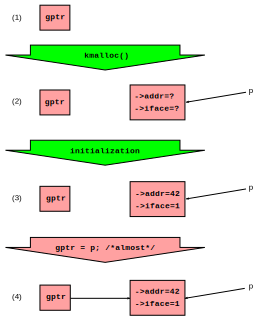
\includegraphics{defer/RCUListInsertClassic}}
\caption{Insertion With Concurrent Readers}
\label{fig:defer:Insertion With Concurrent Readers}
\end{figure}

구현이 가능하긴 한지에 대한 걱정을 최소화 하기 위해, \co{NULL} 이거나 하나의
구조체로의 참조일 하나의 글로벌 포인터로 존재하는 최소한의 데이터 구조에 집중해
봅니다.
이 데이터 구조는 최소한의 것이긴 하지만, 제품 단계에서 상당히 많이 사용되는
것이기도 합니다~\cite{GeoffRomer2018C++DeferredReclamationP0561R4}.
삽입을 위한 고전적 방법이
Figure~\ref{fig:defer:Insertion With Concurrent Readers}
에 보여져 있는데, 위에서 아래로 시간이 흐름에 따라 달라지는 네개의 상태를
보입니다.
첫번째 열은 최초의 상태를 보이는데, \co{gptr} 이 \co{NULL} 입니다.
두번째 열에서, 우리는 물음표로 보여지듯 초기화 되지 않은 이 구조체를
할당합니다.
세번째 열에서, 우린 이 구조체를 초기화 합니다.
마지막으로, 네번째 열에서 우린 \co{gptr} 을 이 새로 할당되고 초기화 된 원소를
참조하도록 업데이트 합니다.

\iffalse

To minimize implementability concerns, we focus on a minimal
data structure, which consists of a single global pointer that is either
\co{NULL} or references a single structure.
Minimal though it might be, this data structure is heavily used in
production~\cite{GeoffRomer2018C++DeferredReclamationP0561R4}.
A classic approach for insertion is shown in
Figure~\ref{fig:defer:Insertion With Concurrent Readers},
which shows four states with time advancing from top to bottom.
The first row shows the initial state, with \co{gptr} equal to \co{NULL}.
In the second row, we have allocated a structure which is uninitialized,
as indicated by the question marks.
In the third row, we have initialized the structure.
Finally, in the fourth and final row, we have updated \co{gptr} to
reference the newly allocated and initialized element.

\fi

우린 이 \co{gptr} 로의 값 할당이 간단한 C-언어의 할당문을 사용할 수 있길 바랄
겁니다.
불행히도,
Section~\ref{sec:toolsoftrade:Shared-Variable Shenanigans}
이 이 바람을 가로막습니다.
따라서, 업데이트 쓰레드는 간단한 C-언어 할당문 대신 이 그림에 보여진 것처럼
\co{smp_store_release()} 또는 뒤에서 보이겠지만 \co{rcu_assign_pointer()} 를
사용해야 합니다.

비슷하게, 어떤 사람들은 읽기 쓰레드가 \co{gptr} 의 값을 얻어오기 위해 하나의
C-언어 할당문을 사용할 수 있기를, 그리고 과거의 값인 \co{NULL} 이나 새로이
설치된 포인터를 읽어와 어떤 경우든 유효한 값을 읽올 것이 보장되기를 바랄
겁니다.
불행히도,
Section~\ref{sec:toolsoftrade:Shared-Variable Shenanigans}
은 이 바람 역시 가로막습니다.
이 보장을 얻기 위해선, 읽기 쓰레드는 그 대신 \co{READ_ONCE()}, 또는, 뒤에서
보이겠지만 \co{rcu_dereference()} 를 사용해야 합니다.
하지만, 대부분의 현대 컴퓨터 시스템에서, 이 읽기 쪽 기능들은 싱글 쓰레드 기반
코드에서 일반적으로 사용될 것과 동일한 하나의 로드 인스트럭션으로 구현될 수
있습니다.

\iffalse

We might hope that this assignment to \co{gptr} could use a simple
C-language assignment statement.
Unfortunately,
Section~\ref{sec:toolsoftrade:Shared-Variable Shenanigans}
dashes these hopes.
Therefore, the updater cannot use a simple C-language assignment, but
must instead use \co{smp_store_release()} as shown in the figure,
or, as will be seen, \co{rcu_assign_pointer()}.

Similarly, one might hope that readers could use a single C-language
assignment to fetch the value of \co{gptr}, and be guaranteed to either
get the old value of \co{NULL} or to get the newly installed pointer,
but either way see a valid result.
Unfortunately, Section~\ref{sec:toolsoftrade:Shared-Variable Shenanigans}
dashes these hopes as well.
To obtain this guarantee, readers must instead use \co{READ_ONCE()},
or, as will be seen, \co{rcu_dereference()}.
However, on most modern computer systems, each of these read-side primitives
can be implemented with a single load instruction, exactly the instruction
that would normally be used in single-threaded code.

\fi

\Cref{fig:defer:Insertion With Concurrent Readers}
를 읽기 쓰레드의 시점에서 다시 보면, 앞의 세개 상태에서 모든 읽기 쓰레드는
\co{gptr} 을 \co{NULL} 값을 갖는 것으로 봅니다.
네번째 상태에 진입하면서, 일부 읽기 쓰레드는 \co{gptr} 이 여전히 \co{NULL} 값을
갖는다고 볼 수 있는 반면 다른 쓰레드들은 새로 설치된 원소를 참조하고 있는
것으로 볼 수 있지만, 어떤 시점 이후로는 모든 읽기 쓰레드가 이 새 원소를 보게 될
겁니다.
항상, 모든 읽기 쓰레드는 \co{gptr} 을 유효한 포인터를 담고 있다고 볼 겁니다.
따라서, 동시의 읽기 쓰레드들이 싱글 쓰레드 기반 코드에서 일반적으로 사용할 것과
동일한 기계 인스트럭션들을 수행하면서 새로운 데이터를 연결된 데이터 구조에
추가하는 것이 정말 가능합니다.
이 동시 읽기에의 비용이 없는 방법은 훌륭한 성능과 확장성을 제공하며, 리얼타임
사용처에서 뛰어나게 잘 사용될 수 있습니다.

\iffalse

Reviewing \cref{fig:defer:Insertion With Concurrent Readers}
from the viewpoint of readers, in the first three states all readers
see \co{gptr} having the value \co{NULL}.
Upon entering the fourth state, some readers might see \co{gptr} still
having the value \co{NULL} while others might see it referencing the
newly inserted element, but after some time, all readers will see this
new element.
At all times, all readers will see \co{gptr} as containing a valid pointer.
Therefore, it really is possible to add new data to linked data structures
while allowing concurrent readers to execute the same sequence of machine
instructions that is normally used in single-threaded code.
This no-cost approach to concurrent reading provides excellent performance
and scalability, and also is eminently suitable for real-time use.

\fi

\begin{figure}[tb]
\centering
\resizebox{3in}{!}{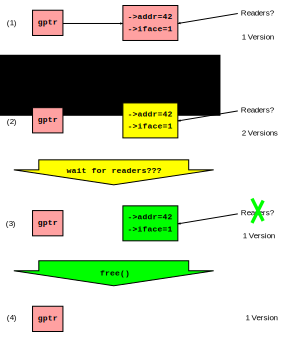
\includegraphics{defer/RCUListDeleteClassic}}
\caption{Deletion With Concurrent Readers}
\label{fig:defer:Deletion With Concurrent Readers}
\end{figure}

삽입은 물론 상당히 유용합니다만, 금방이든 더 나중이든, 데이터를 지워야 하기도
할 겁니다.
Figure~\ref{fig:defer:Deletion With Concurrent Readers}
에 보이듯, 첫번째 단계는 쉽습니다.
Section~\ref{sec:toolsoftrade:Shared-Variable Shenanigans}
에서의 교훈을 다시 상기해 보면, \co{smp_store_release()} 가 이 포인터를
\co{NULL} 로 만들기 위해 사용되어, 이 그림의 첫번째 열에서 두번째 열로
넘어갑니다.
이 시점에서, 기존부터 존재하던 읽기 쓰레드는 \co{->addr} 는 42 값을 그리고
\co{->iface} 는 1 값을 갖는 것으로 볼 수 있지만, 새로 시작된 읽기 쓰레드는
\co{NULL} 포인터를 볼 것으로, 즉 동시의 읽기 쓰레드들이 이 그림의 ``2
Versions'' 로 표시된 것처럼 현 상태에 대해 다른 의견을 가질 수 있습니다.

\iffalse

Insertion is of course quite useful, but sooner or later, it will also
be necessary to delete data.
As can be seen in
Figure~\ref{fig:defer:Deletion With Concurrent Readers},
the first step is easy.
Again taking the lessons from
Section~\ref{sec:toolsoftrade:Shared-Variable Shenanigans}
to heart, \co{smp_store_release()} is used to \co{NULL} the pointer,
thus moving from the first row to the second in the figure.
At this point, pre-existing readers see the old structure with
\co{->addr} of 42 and \co{->iface} of 1, but new readers will see
a \co{NULL} pointer, that is, concurrent readers can disagree on
the state, as indicated by the ``2 Versions'' in the figure.

\fi

\QuickQuizSeries{%
\QuickQuizB{
	Figure~\ref{fig:defer:Deletion With Concurrent Readers}
	는 \co{NULL} 포인터를 저장하는데 왜 \co{smp_store_release()} 를
	사용하나요?
	\co{NULL} 포인터 저장에 대해 순서지을 구조체 초기화가 없다는 점을
	감안하면 \co{WRITE_ONCE()} 만으로도 이 경우에는 괜찮지 않을까요?

	\iffalse

	Why does
	Figure~\ref{fig:defer:Deletion With Concurrent Readers}
	use \co{smp_store_release()} given that it is storing
	a \co{NULL} pointer?
	Wouldn't \co{WRITE_ONCE()} work just as well in this case,
	given that there is no structure initialization to order
	against the store of the \co{NULL} pointer?

	\fi

}\QuickQuizAnswerB{
	맞아요, 그럴 겁니다.

	\co{NULL} 포인터가 할당되고 있을 뿐, 순서지을 것이 존재하지 않으므로,
	\co{smp_store_release()} 를 사용할 필요는없습니다.
	대조적으로, \co{NULL} 이 아닌 포인터를 할당할 때에는 그 포인터로
	가리켜지는 구조체의 초기화가 이 포인터의 할당 전에 행해졌음을 분명히
	하기 위해 \co{smp_store_release()} 가 사용되어야 합니다.

	짧게 말해서, \co{WRITE_ONCE()} 는 동작할 것이고, 어떤 아키텍쳐에서는
	약간의 CPU 시간을 아낄 겁니다.
	하지만, 뒤에서 보게 되겠지만, 소프투에어 엔지니어링 관점의 걱정은
	\co{smp_store_release()} 와 상당히 유사한 \co{rcu_assign_pointer()}
	라는 특수한 기능의 사용을 장려할 겁니다.

	\iffalse

	Yes, it would.

	Because a \co{NULL} pointer is being assigned, there is nothing
	to order against, so there is no need for \co{smp_store_release()}.
	In contrast, when assigning a non-\co{NULL} pointer, it is
	necessary to use \co{smp_store_release()} in order to ensure
	that initialization of the pointed-to structure is carried
	out before assignment of the pointer.

	In short, \co{WRITE_ONCE()} would work, and would
	save a little bit of CPU time on some architectures.
	However, as we will see, software-engineering concerns
	will motivate use of a special \co{rcu_assign_pointer()}
	that is quite similar to \co{smp_store_release()}.

	\fi

}\QuickQuizEndB
%
\QuickQuizE{
	동시에 수행되는 읽기 쓰레드는
	Figure~\ref{fig:defer:Deletion With Concurrent Readers}
	에 그려진 수행 순서에 따르면 \co{gptr} 의 값에 대해 동의하지 않을 수
	있습니다.
	이건 뭔가 문제있지 않나요???

	\iffalse

	Readers running concurrently each other and with the procedure
	outlined in
	Figure~\ref{fig:defer:Deletion With Concurrent Readers}
	can disagree on the value of \co{gptr}.
	Isn't that just a wee bit problematic???

	\fi

}\QuickQuizAnswerE{
	꼭 그렇진 않습니다.

	Section~\ref{sec:cpu:Hardware Optimizations}
	와~\ref{sec:cpu:Hardware Free Lunch?}
	에서 힌트가 주어진 것처럼, 빛의 속도의 지연은 컴퓨터의 데이터는 그
	데이터가 실제로 모델링 하고자 의도된 바깥의 사실에 비교해서는 항상
	오래되어 있습니다.

	따라서 실제 세계의 알고리즘은 외부의 현실과 그 현실을 반영하는 컴퓨터
	내부 데이터의 비일관성을 감내해야만 합니다.
	이런 알고리즘들 여럿은 컴퓨터 내부 데이터에서의 비일관성도 어느정도는
	감내할 수 있습니다.
	Section~\ref{sec:datastruct:RCU-Protected Hash Table Discussion}
	이 이 점을 더 자세히 다룹니다.

	\iffalse

	Not necessarily.

	As hinted at in Sections~\ref{sec:cpu:Hardware Optimizations}
	and~\ref{sec:cpu:Hardware Free Lunch?},
	speed-of-light delays mean that a computer's data is always
	stale compared to whatever external reality that data is intended
	to model.

	Real-world algorithms therefore absolutely must tolerate
	inconsistancies between external reality and the in-computer
	data reflecting that reality.
	Many of those algorithms are also able to tolerate some degree
	of inconsistency within the in-computer data.
	Section~\ref{sec:datastruct:RCU-Protected Hash Table Discussion}
	discusses this point in more detail.

	\fi

	이런 비일관적이고 오래된 데이터를 감내해야 하는 필요성은 RCU 에만
	국한되지 않는다는 점을 알아두시기 바랍니다.
	이는 레퍼런스 카운팅, 해저드 포인터, 시퀀스 락, 그리고 심지어 일부 락킹
	사용 예에도 적용됩니다.
	예를 들어, 여러분이 락을 잡은 채 어떤 값을 계산하지만 그 값을 해당 락을
	해제한 후 사용한다면, 여러분은 오래된 데이터를 사용하고 있을 수
	있습니다.
	어쨌건, 그 값이 기반하고 있는 데이터는 그 락이 해제되는 순간 어떻게든
	변할 수도 있습니다.

	그러니, 그렇습니다, RCU 읽기 쓰레드는 오래되고 비일관적인 데이터를 볼
	수 있습니다, 하지만 아니요, 이게 문제여야만 할 이유는 없어요.
	그리고 필요하다면 그런 오래되고 비일관적인 데이터 문제를 막을 수 있는
	RCU 사용 패턴도 있습니다~\cite{Arcangeli03}.

	\iffalse

	Please note that this need to tolerate inconsistent and stale
	data is not limited to RCU\@.
	It also applies to reference counting, hazard pointers, sequence
	locks, and even to some locking use cases.
	For example, if you compute some quantity while holding a lock,
	but use that quantity after releasing that lock,
	you might well be using stale data.
	After all, the data that quantity is based on might change
	arbitrarily as soon as the lock is released.

	So yes, RCU readers can see stale and inconsistent data, but no,
	this is not necessarily problematic.
	And, when needed, there are RCU usage patterns that avoid both
	staleness and inconsistency~\cite{Arcangeli03}.

	\fi

}\QuickQuizEndE
}

우린 열~3 에서 볼 수 있듯 모든 기존부터 존재한 읽기 쓰레드들이 완료하길
기다리는 것만으로 단일 버전으로 돌아올 수 있습니다.
이 지점에서, 모든 기존부터 존재하던 읽기 쓰레드는 종료되었고, 뒤따르는 읽기
쓰레드는 어느 것도 기존 데이터 아이템으로의 경로를 갖지 못하므로, 그걸 참조하는
어떤 읽기 쓰레드도 존재할 수 없습니다.
따라서 그 아이템은 열~4 에서 보여지듯 안전히 메모리 해제될 수 있습니다.

따라서, 기존부터 존재한 읽기 쓰레드들이 완료되길 기다릴 방법이 존재한다면
읽기 쓰레드들이 싱글 쓰레드 수행 시에나 적합할 것과 동일한 기계
인스트럭션들만을 수행하면서도 연결된 데이터 구조에 데이터를 추가할 수도 삭제할
수도 있습니다.
그러니 앞서 했던 것들이 너무 멀리 간 것만은 아닐수도 있습니다!

하지만 어떻게 기존부터 존재한 읽기 쓰레드들이 실제로 완료되었다고 이야기 할 수
있을까요?
이 질문이 다음 섹션의 주제입니다.

\iffalse

We get back to a single version simply by waiting for all the
pre-existing readers to complete, as shown in row~3.
At that point, all the pre-existing readers are done, and no later
reader has a path to the old data item, so there can no longer be
any readers referencing it.
It may therefore be safely freed, as shown on row~4.

Thus, given a way to wait for pre-existing readers to complete,
it is possible to both add data to and remove data from a linked
data structure, despite the readers executing the same sequence
of machine instructions that would be appropriate for single-threaded
execution.
So perhaps going all the way was not too far after all!

But how can we tell when all of the pre-existing readers have in
fact completed?
This question is the topic of the next section.

\fi

\subsubsection{Waiting for Readers}
\label{sec:defer:Waiting for Readers}

읽기 쓰레드의 기다리기를 레퍼런스 카운팅 기반으로 하고 싶을 수 있겠습니다만,
Chapter~\ref{chp:Counting}
의
Figure~\ref{fig:count:Atomic Increment Scalability on x86}
는 현재의 레퍼런스 카운팅은
Section~\ref{sec:defer:Reference Counting}
에서 이미 보았듯 굉장한 오버헤드를 초래함을 보았습니다.
해저드 포인터는 이 오버헤드를 상당히 줄입니다만, 우리가
Section~\ref{sec:defer:Hazard Pointers}
에서 보았듯이, 완전히 없애진 못합니다.
그렇다고는 하나, 많은 RCU 구현이 매우 주의 깊은 캐시 지역적 카운터의 사용을
합니다.

\iffalse

It is tempting to base reader waiting on reference counting, but
Figure~\ref{fig:count:Atomic Increment Scalability on x86}
in
Chapter~\ref{chp:Counting}
shows that concurrent reference counting results in extreme overhead,
as we already saw in
Section~\ref{sec:defer:Reference Counting}.
Hazard pointers profoundly reduce this overhead, but, as we saw in
Section~\ref{sec:defer:Hazard Pointers}, not to zero.
Nevertheless, many RCU implementations make very careful cache-local
use of counters.

\fi

두번째 접근법은 메모리 동기화가 비쌈을 파악하고, 따라서 레지스터를 대신
사용하는데, 이는 각 CPU 또는 쓰레드의 프로그램 카운터 (PC) 로, 따라서 읽기
쓰레드에게는 적어도 동시의 업데이트의 부재 시에는 오버헤드를 일으키지 않습니다.
업데이트 쓰레드는 각 적절한 PC 를 반복적으로 살펴보고, 그 PC 가 읽기 쪽 코드
내에 위치해 있지 않다면, 연관된 CPU 또는 쓰레드는 조용한 상태 (quiescent state)
에 있는 것이며, 따라서 이는 새로이 제거된 데이터 원소로의 액세스를 할수도 있는
읽기 쓰레드는 모두 완료되었다는 신호가 됩니다.
모든 CPU 또는 쓰레드의 PC 가 모두 모든 읽기 쓰레드의 바깥에 있음이 확인된다면,
이 유예 기간 (grace period) 가 완료됩니다.
이 방법은 몇가지 심각한 기술적 어려움도 가지고 있는데, 메모리 순서 맞추기, 읽기
쓰레드에 의해 \emph{가끔} 호출되는 함수들, 그리고 항상 신나는 코드 모습
최적화가 포함됩니다.
그러나, 이 방법은 제품 단계에서 사용되었다고 이야기
됩니다~\cite{MikeAsh2015Apple}.

\iffalse

A second approach observes that memory synchronization is expensive,
and therefore uses registers instead, namely each CPU's or thread's
program counter (PC), thus imposing no overhead on readers, at least
in the absence of concurrent updates.
The updater polls each relevant PC, and if that PC is not within read-side
code, then the corresponding CPU or thread is within a quiescent state,
in turn signaling the completion of any reader that might have access
to the newly removed data element.
Once all CPU's or thread's PCs have been observed to be outside of any
reader, the grace period has completed.
Please note that this approach poses some serious challenges, including
memory ordering, functions that are \emph{sometimes} invoked from readers,
and ever-exciting code-motion optimizations.
Nevertheless, this approach is said to be used in
production~\cite{MikeAsh2015Apple}.

\fi

세번째 접근법은 모든 합리적 읽기 쓰레드의 수명을 충분히 넘어설 정도로 긴 고정된
시간동안 그냥 기다리는 것입니다~\cite{Jacobson93,AjuJohn95}.
이는 하드 리얼타임 시스템에서는 잘 동작합니다만~\cite{YuxinRen2018RTRCU},
그보다 덜 진귀한 환경에서라면, Murphy 는 비합리적일 정도로 오래 살아있는 읽기
쓰레드에도 준비해야 하는게 무척 중요하다고 말합니다.
이를 자세히 보기 위해, 그러는데 실패했을 때의 결과를 생각해 봅시다:
어떤 데이터 항목은 이 비합리적인 읽기 쓰레드가 여전히 그것을 참조하고 있는 동안
메모리 해제될 수 있고, 그 항목은 곧바로 재할당되어 심지어 다른 타입의 데이터
항목으로 사용되고 있을 수 있습니다.
그러면 이 비합리적 읽기 쓰레드와 부주의한 재할당자는 같은 메모리를 두개의 매우
다른 목적으로 사용하려 할 것입니다.
그 결과는 디버깅 하기에 무척 어려울 것입니다.

\iffalse

A third approach is to simply wait for a fixed period of time that is
long enough to comfortably exceed the lifetime of any reasonable
reader~\cite{Jacobson93,AjuJohn95}.
This can work quite well in hard real-time systems~\cite{YuxinRen2018RTRCU},
but in less exotic
settings, Murphy says that it is critically important to be prepared
even for unreasonably long-lived readers.
To see this, consider the consequences of failing do so:
A data item will be freed while the unreasonable reader is still
referencing it, and that item might well be immediately reallocated,
possibly even as a data item of some other type.
The unreasonable reader and the unwitting reallocator would then
be attempting to use the same memory for two very different purposes.
The ensuing mess will at best be exceedingly difficult to debug.

\fi

네번째 접근법은 영원히 기다리는 것으로, 그렇게 하는게 가장 비합리적인 읽기
쓰레드조차도 처리해 줄 것이라는 점에서 안전합니다.
이 접근법은 또한 ``메모리 누출'' 이라고도 불리며, 메모리 누출은 시기 상조의
그리고 불편한 리부팅을 요구한다는 사실 때문에 나쁜 평판을 가지고 있습니다.
그러나, 이는 업데이트 비율과 시스템 가동시간이 모두 꽤 정확히 그 한계가 정해져
있을 때라면 사용될 수 있는 전략입니다.
예를 들어, 이 방법은 시스템이 높은 가용성을 가진 클러스터여서 이 클러스터가
정말로 높은 가용성을 유지한다는 것을 분명히 하기 위해 주기적으로 고장나는
것이라면 잘 동작할 수 있습니다.\footnote{
	이 주기적 고장을 강제하는 프로그램은 가끔 ``chaos monkey'' 라고
	불립니다:
	\url{https://netflix.github.io/chaosmonkey/}.
	하지만, 너무 오래 수행되는 시스템에 의해 야기되는 혼란을 무시하는 것도
	실수가 될수도 있습니다.}
메모리를 누출하는 것은 또한 garbage collector 를 가진 경우에도 사용될 수
있을텐데, 이 경우는 garbage collector 가 이 누출을 막는 것으로 생각될 수
있습니다~\cite{Kung80}.
하지만, 여러분의 환경이 garbage collector 를 지원하지 않는다면, 마저
읽으십시오!

\iffalse

A fourth approach is to wait forever, secure in the knowledge that
doing so will accommodate even the most unreasonable reader.
This approach is also called ``leaking memory'', and has a bad reputation
due to the fact that memory leaks often require untimely and
inconvenient reboots.
Nevertheless, this is a viable strategy when the update rate and the
uptime are both sharply bounded.
For example, this approach could work well in a high-availability
cluster where systems were periodically crashed in order to ensure
that cluster really remained highly available.\footnote{
	The program that forces the periodic crashing is sometimes
	known as a ``chaos monkey'':
	\url{https://netflix.github.io/chaosmonkey/}.
	However, it might also be a mistake to neglect chaos caused
	by systems running for too long.}
Leaking the memory is also a viable strategy in environments having
garbage collectors, in which case the garbage collector can be thought
of as plugging the leak~\cite{Kung80}.
However, if your environment lacks a garbage collector, read on!

\fi

다섯번째 접근법은 전통적 세상을-멈추기 (stop-the-world) garbage collector 에
의해 예시되는 주기적으로 ``세상을 멈추기'' 를 사용해 주기적 고장내기를
막습니다.
이 방법은 또한 각 일하는 날의 끝마다 시스템의 전원을 끄는게 일반적 행동이었던,
어디나 있는 연결성 전의 수십년간 많이 사용되었습니다.
하지만, 오늘날의 항상 연결되어 있고 항상 켜져있는 세상에서는, 세상을 멈추기는
응답 시간을 크게 악화시킬 수 있는데, 이는 동시적 garbage collector 의 개발의
모티베이션 중 하나가 되었습니다~\cite{DavidFBacon2003RTGC}.
더 나아가, 우린 모든 앞서서부터 존재하고 있는 읽기 쓰레드가 모두 완료되기를
기다려야 하기는 하지만, 그것들이 동시에 완료되어야 할 필요는 없습니다.

\iffalse

A fifth approach avoids the period crashes in favor of periodically
``stopping the world'', as exemplified by the traditional stop-the-world
garbage collector.
This approach was also heavily used during the decades before
ubiquitous connectivity, when it was common practice to power systems
off at the end of each working day.
However, in today's always-connected always-on world, stopping the world
can gravely degrade response times, which has been one motivation for the
development of concurrent garbage collectors~\cite{DavidFBacon2003RTGC}.
Furthermore, although we need all pre-existing readers to complete, we do
not need them all to complete at the same time.

\fi

이 발견은 여섯번째 접근법을 이끌어내는데, 한번에 한 CPU 또는 쓰레드를 멈추는
것입니다.
이 방법은 읽기 쓰레드의 응답 시간을 전혀 악화시키지 않는다는 장점을 갖습니다.
더 나아가서, 많은 어플리케이션들이 이미 앞의 앞서서부터 존재하고 있는 읽기
스레드들이 모두 완료된 후에만 도달할 수 있는 상태 (\emph{quiescent state} 라
불립니다) 를 갖습니다.
트랜잭션 처리 시스템에서는, 한쌍의 연속된 트랜잭션 사이의 시간이 quiescent
state 일 수 있습니다.
반응형 시스템에서는, 연속된 한 쌍의 이벤트 사이의 상태가 quiescent state 일
겁니다.
Preemption 기반이지 않은 운영체제 커널에서는, 컨텍스트 스위치가 quiescent state
가 될 수 있습니다~\cite{McKenney98}.
어떤 형태든, 모든 CPU 그리고/또는 쓰레드가 하나의 quiescent state 를 지난다면,
이 시스템은 하나의 \emph{grace period} 를 완료했다고 이야기 되며, 이 지점에서는
이 grace period 의 시작 시점에서 존재했던 모든 읽기 쓰레드는 완료되었다는게
보장됩니다.
그 결과, 이 grace period 의 시작 전에 제거된 데이터 항목들은 메모리 해제되기에
안전합니다.\footnote{
	RCU 는 단순히 메모리 회수 미루기보다 훨씬 많은 걸 할 수 있으나, 
	회수 미루기는 RCU 의 가장 흔한 사용예이며, 따라서 시작하기에 훌륭한
	지점입니다.}

\iffalse

This observation leads to the sixth approach, which is stopping
one CPU or thread at a time.
This approach has the advantage of not degrading reader response times
at all, let alone gravely.
Furthermore, numerous applications already have states (termed
\emph{quiescent states}) that can be
reached only after all pre-existing readers are done.
In transaction-processing systems, the time between a pair of
successive transactions might be a quiescent state.
In reactive systems, the state between a pair of successive events
might be a quiescent state.
Within non-preemptive operating-systems kernels, a context switch can be
a quiescent state~\cite{McKenney98}.
Either way, once all CPUs and/or threads have passed through a quiescent
state, the system is said to have completed a \emph{grace period},
at which point all readers in existence at the start of that grace period
are guaranteed to have completed.
As a result, it is also guaranteed to be safe to free any removed data
items that were removed prior to the start of that grace period.\footnote{
	It is possible to do much more with RCU than simply defer
	reclamation of memory, but deferred reclamation is RCU's most
	common use case, and is therefore an excellent place to start.}

\fi

Preemption 이 없는 운영체제 커널에서 컨텍스트 스위치가 유효한 quiescent state 가 되려면 읽기 쓰레드는
Figure~\ref{fig:defer:Insertion With Concurrent Readers}
와~\ref{fig:defer:Deletion With Concurrent Readers}
의 \co{gptr} 포인터에 의해 얻어지는 데이터 구조 인스턴스를 참조하는 동안은
블록킹 되는 걸 방지해야만 합니다.
이 블록킹 방지 제약은 순수 스핀락에서도 비슷한 제약으로 존재하는데, 여기선 CPU
는 스핀락을 잡고 있는 동안 블록킹 되는게 금지됩니다.
이 제약이 없다면, 모든 CPU 는 블록된 쓰레드에 의해 잡혀 있는 스핀락을 획득하려
스핀하는 쓰레드들에 의해 소모될 수 있습니다.
이 스핀하는 쓰레드들은 그것들이 이 락을 획득하기 전까지는 CPU 를 놓지 않을
것이지만, 이 락을 쥐고 있는 쓰레드는 이 스핀하고 있는 쓰레드들 중 하나가 CPU 를
하나라도 놓기 전까지는 이 락을 놓아주지 못할 겁니다.
이는 고전적 데드락 환경이며, 이 데드락은 스핀락을 잡고 있는 동안은 블록킹을
방지하는 것으로 막아집니다.

\iffalse

Within a non-preemptive operating-system kernel, for context switch to be
a valid quiescent state, readers must be prohibited from blocking while
referencing a given instance data structure obtained via the \co{gptr}
pointer shown in
Figures~\ref{fig:defer:Insertion With Concurrent Readers}
and~\ref{fig:defer:Deletion With Concurrent Readers}.
This no-blocking constraint is consistent with similar constraints
on pure spinlocks, where a CPU is forbidden from blocking while
holding a spinlock.
Without this constraint, all CPUs might be consumed by threads
spinning attempting to acquire a spinlock held by a blocked thread.
The spinning threads will not relinquish their CPUs until they acquire
the lock, but the thread holding the lock cannot possibly release it
until one of the spinning threads relinquishes a CPU\@.
This is a classic deadlock situation, and this deadlock is avoided
by forbidding blocking while holding a spinlock.

\fi

다시, 이 동일한 제약이 \co{gptr} 을 역참조하는 읽기 쓰레드에게도 적용됩니다:
그런 쓰레드는 그것들이 이 가리켜진 데이터 항목을 사용하는 것을 마무리 하기
전까지는 블록되지 않아야 합니다.
업데이트 쓰레드가 막 \co{smp_store_release()} 를 수행하는 것을 완료한
Figure~\ref{fig:defer:Deletion With Concurrent Readers}
의 두번째 열로 돌아와서, CPU~0 이 컨텍스트 스위치를 했다고 생각해 봅시다.
읽기 쓰레드는 이 링크드 리스트를 순회하는 동안은 블록되는 것이 허용되지
않았으므로, 우린 CPU~0 에서 수행되었을 수도 있는 모든 앞의 읽기 쓰레드들이
완료되었다고 보장됩니다.
이 논리를 다른 CPU 들로 확장하면, 각 CPU 가 모두 컨텍스트 스위치 수행을
목격했다면, 모든 앞의 읽기 쓰레드가 완료되었음이, 새로이 제거된 데이터 원소를
참조하고 있는 어떤 읽기 쓰레드도 더이상 존재하지 않음이 보장됩니다.
그럼 이 업데이트 쓰레드는 안전하게 이 데이터 원소를 메모리 해제할 수 있어,
Figure~\ref{fig:defer:Deletion With Concurrent Readers}
의 가장 아래에 보인 상태에 도달합니다.

\iffalse

Again, this same constraint is imposed on reader threads dereferencing
\co{gptr}: such threads are not allowed to block until after
they are done using the pointed-to data item.
Returning to the second row of
Figure~\ref{fig:defer:Deletion With Concurrent Readers},
where the updater has just completed executing the \co{smp_store_release()},
imagine that CPU~0 executes a context switch.
Because readers are not permitted to block while traversing the linked
list, we are guaranteed that all prior readers that might have been running on
CPU~0 will have completed.
Extending this line of reasoning to the other CPUs, once each CPU has
been observed executing a context switch, we are guaranteed that all
prior readers have completed, and that there are no longer any reader
threads referencing the newly removed data element.
The updater can then safely free that data element, resulting in the
state shown at the bottom of
Figure~\ref{fig:defer:Deletion With Concurrent Readers}.

\fi

\begin{figure}[tb]
\centering
\resizebox{3in}{!}{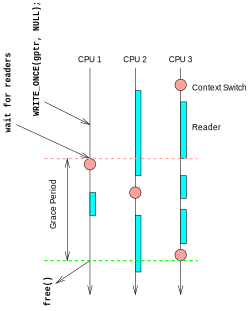
\includegraphics{defer/QSBRGracePeriod}}
\caption{QSBR: Waiting for Pre-Existing Readers}
\label{fig:defer:QSBR: Waiting for Pre-Existing Readers}
\end{figure}

이 방법은 \emph{quiescent state based reclamation}
(QSBR)~\cite{ThomasEHart2006a} 라고 명명되었습니다.
하나의 QSBR 방법이
Figure~\ref{fig:defer:QSBR: Waiting for Pre-Existing Readers}
에 시간이 이 그림의 꼭대기에서 아래로 흐르는 모습으로 그려져 있습니다.
CPU~1 은 현재 데이터 항목을 제거하는 \co{WRITE_ONCE()} 를 수행하고 (아마도 이
포인터 값을 앞서 읽었고 자신을 적절한 동기화를 하고 있게 했을 겁니다), 읽기
쓰레드를 기다립니다.
이 대기 오퍼레이션은 즉각적인 컨텍스트 스위치를 초래하는데, 이는 quiescent
state 로 (핑크색 원으로 표시되어 있습니다), CPU~1 에서의 모든 앞선 읽기는
완료되었음을 의미합니다.
이어서, CPU~2 가 컨텍스트 스위치를 하여, CPU~1 과~2 의 모든 읽기 쓰레드는 이제
완료되었음이 알려집니다.
마지막으로, CPU~3 이 컨텍스트 스위치를 합니다.
이 지점에서, 전체 시스템의 모든 읽기 쓰레드는 완료되었음이 알려지며, 따라서
grace period 가 종료되어 CPU~1 이 오래된 데이터 항목을 메모리 해제하는 것을
허용합니다.

\iffalse

This approach is termed \emph{quiescent state based reclamation}
(QSBR)~\cite{ThomasEHart2006a}.
A QSBR schematic is shown in
Figure~\ref{fig:defer:QSBR: Waiting for Pre-Existing Readers},
with time advancing from the top of the figure to the bottom.
CPU~1 does the \co{WRITE_ONCE()} that removes the current data
item (presumably having previously read the pointer value and
availed itself of appropriate synchronization), then waits
for readers.
This wait operation results in an immediate context switch, which is a
quiescent state (denoted by the pink circle), which in turn means that
all prior reads on CPU~1 have completed.
Next, CPU~2 does a context switch, so that all readers on CPUs~1 and~2
are now known to have completed.
Finally, CPU~3 does a context switch.
At this point, all readers throughout the entire system are known to
have completed, so the grace period ends, permitting CPU~1 to free
the old data item.

\fi

\QuickQuiz{
	Figure~\ref{fig:defer:QSBR: Waiting for Pre-Existing Readers} 에서,
	CPU~3 의 이 오래된 데이터 항목으로의 액세스를 했을 수 있는 읽기
	쓰레드는 이 grace period 가 시작하기도 전에 이미 완료되었어요!
	그런데 왜 CPU~3 의 마지막 컨텍스트 스위치를 신경쓰나요???

	\iffalse

	In Figure~\ref{fig:defer:QSBR: Waiting for Pre-Existing Readers},
	the last of CPU~3's readers that could possibly have
	access to the old data item ended before the grace period
	even started!
	So why would anyone bother waiting until CPU~3's later context
	switch???

	\fi

}\QuickQuizAnswer{
	이 대기는 읽기 쓰레드들이 싱글쓰레드 상황에서나 적절한 것과 똑같은
	인스트럭션들을 사용할 수 있게 해주기 때문입니다.
	달리 말하자면, 이 추가적인 ``과잉의'' 대기가 읽기 쪽의 훌륭한 성능,
	확장성, 그리고 리얼타임 응답을 가능하게 합니다.

	\iffalse

	Because that waiting is exactly what enables readers to use
	the same sequence of instructions that is appropriate for
	single-theaded situations.
	In other words, this additional ``redundant'' waiting enables
	excellent read-side performance, scalability, and real-time
	response.

	\fi

}\QuickQuizEnd

\subsubsection{Toy Implementation}
\label{sec:defer:Toy Implementation}

제품 수준 QSBR 구현은 무척 복잡할 수 있지만, preemption 기반이 아닌 리눅스
커널에서의 장난감 수준 구현은 굉장히 간단합니다:

\iffalse

Although production-quality QSBR implementations can be quite complex,
a toy non-preemptive Linux-kernel implementation is exceedingly simple:

\fi

\begin{VerbatimN}[samepage=true]
void synchronize_rcu(void)
{
	int cpu;

	for_each_online_cpu(cpu)
		sched_setaffinity(current->pid, cpumask_of(cpu));
}
\end{VerbatimN}

\co{for_each_online_cpu()} 기능은 모든 CPU 를 순회하고,
\co{sched_setaffinity()} 함수는 현재 쓰레드가 명시된 CPU 에서 수행되게 하는데,
이는 이 대상 CPU 가 컨텍스트 스위치를 수행하게끔 강제합니다.
따라서, \co{for_each_online_cpu()} 가 완료되고 나면, 각 CPU 는 한번의 컨텍스트
스위치는 수행한 것인데, 이는 곧 모든 앞서서부터 존재해온 읽기 쓰레드가 모두
완료되었음을 보장합니다.

\iffalse

The \co{for_each_online_cpu()} primitive iterates over all CPUs, and
the \co{sched_setaffinity()} function causes the current thread to
execute on the specified CPU, which forces the destination CPU to execute
a context switch.
Therefore, once the \co{for_each_online_cpu()} has completed, each CPU
has executed a context switch, which in turn guarantees that
all pre-existing reader threads have completed.

\fi

\begin{listing}[tbp]
\begin{fcvlabel}[ln:defer:Insertion and Deletion With Concurrent Readers]
\begin{VerbatimL}[commandchars=\\\[\]]
struct route *gptr;

int access_route(int (*f)(struct route *rp))
{
	int ret = -1;
	struct route *rp;

	rcu_read_lock();
	rp = rcu_dereference(gptr);
	if (rp)
		ret = f(rp);		\lnlbl[access_rp]
	rcu_read_unlock();
	return ret;
}

struct route *ins_route(struct route *rp)
{
	struct route *old_rp;

	spin_lock(&route_lock);
	old_rp = gptr;
	rcu_assign_pointer(gptr, rp);
	spin_unlock(&route_lock);
	return old_rp;
}

int del_route(void)
{
	struct route *old_rp;

	spin_lock(&route_lock);
	old_rp = gptr;
	RCU_INIT_POINTER(gptr, NULL);
	spin_unlock(&route_lock);
	synchronize_rcu();
	free(old_rp);
	return !!old_rp;
}
\end{VerbatimL}
\end{fcvlabel}
\caption{Insertion and Deletion With Concurrent Readers}
\label{lst:defer:Insertion and Deletion With Concurrent Readers}
\end{listing}

이 방법은 제품 수준이 \emph{아님을} 알아 두시기 바랍니다.
여러개의 특수 상황에 대한 처리와 여러개의 강력한 최적화의 필요는 제품 수준
구현이 무척 복잡함을 의미합니다.
이에 더해, preemption 기반 환경을 위한 RCU 구현은 읽기 쓰레드가 실제로 무언가를
더할 것을 필요로 하는데, 리얼타임이 아닌 리눅스 커널 환경에서는
\co{rcu_read_lock()} 과 \co{rcu_read_unlock()} 을 각각 \co{preempt_disable()}
과 \co{preempt_enable()} 로 간단히 정의하는 것으로 될 수 있습니다.\footnote{
	Preemption 되는 읽기쪽 크리티컬 섹션을 다루는 어떤 장난감 수준 RCU
	구현들이 Appendix~\ref{chp:app:``Toy'' RCU Implementations} 에 보여져
	있습니다.}
그러나, 이 간단한 preemption 불가 방법은 이론적으로 완벽하며, 읽기 쪽 동기화를
동시의 업데이트가 있음에도 불구하고 비용 없이 제공하는게 가능함을 보입니다.
실제로,
Listing~\ref{lst:defer:Insertion and Deletion With Concurrent Readers}
은 어떻게 읽기 (\co{access_route()}),
Figure~\ref{fig:defer:Insertion With Concurrent Readers} 의 삽입,
(\co{ins_route()})
Figure~\ref{fig:defer:Deletion With Concurrent Readers} 의 삭제가
(\co{del_route()} 구현될 수 있는지 보입니다.
(약간 더 그럴싸한 라우팅 테이블은
Section~\ref{sec:defer:RCU for Pre-BSD Routing} 에 보여져 있습니다.)

\iffalse

Please note that this approach is \emph{not} production quality.
Correct handling of a number of corner cases and the need for a number
of powerful optimizations mean that production-quality implementations
are quite complex.
In addition, RCU implementations for preemptible environments
require that readers actually do something, which in non-real-time
Linux-kernel environments can be as simple as defining
\co{rcu_read_lock()} and \co{rcu_read_unlock()} as \co{preempt_disable()}
and \co{preempt_enable()}, respectively.\footnote{
	Some toy RCU implementations that handle preempted
	read-side critical sections are shown in
	Appendix~\ref{chp:app:``Toy'' RCU Implementations}.}
However, this simple non-preemptible approach is conceptually complete,
and demonstrates that it really is possible to provide read-side
synchronization at zero cost, even in the face of concurrent updates.
In fact,
Listing~\ref{lst:defer:Insertion and Deletion With Concurrent Readers}
shows how reading (\co{access_route()}),
Figure~\ref{fig:defer:Insertion With Concurrent Readers}'s
insertion (\co{ins_route()}) and
Figure~\ref{fig:defer:Deletion With Concurrent Readers}'s
deletion (\co{del_route()}) can
be implemented.
(A slightly more capable routing table is shown in
Section~\ref{sec:defer:RCU for Pre-BSD Routing}.)

\fi

\QuickQuizSeries{%
\QuickQuizB{
	Listing~\ref{lst:defer:Insertion and Deletion With Concurrent Readers}
	의 \co{rcu_read_lock()} 과 \co{rcu_read_unlock()} 의 요점이 뭔가요?
	이 quiescent state 들이 스스로 자신을 이야기하게 하는건 어떤가요?

	\iffalse

	What is the point of \co{rcu_read_lock()} and \co{rcu_read_unlock()} in
	Listing~\ref{lst:defer:Insertion and Deletion With Concurrent Readers}?
	Why not just let the quiescent states speak for themselves?

	\fi

}\QuickQuizAnswerB{
	읽기 쓰레드들은 quiescent state 를 가로지를 수 없음을 기억하세요.
	예를 들어, 리눅스 커널에서 RCU 읽기 쓰레드는 컨텍스트 스위치를 수행할
	수 없습니다.
	\co{rcu_read_lock()} 과 \co{rcu_read_unlock()} 의 사용은 올바르지 않게
	위치된 quiescent state 들을 디버깅 할 수 있게 하고, 그러지 않으면 찾기
	어렵고 간헐적으로 나타나며 무척 파괴적인 버그를 찾기 쉽게 해줍니다.

	\iffalse

	Recall that readers are not permitted to pass through a quiescent
	state.
	For example, within the Linux kernel, RCU readers are not permitted
	to execute a context switch.
	Use of \co{rcu_read_lock()} and \co{rcu_read_unlock()} enables
	debug checks for improperly placed quiescent states, making it
	easy to find bugs that would otherwise be difficult to find,
	intermittent, and quite destructive.

	\fi

}\QuickQuizEndB
%
\QuickQuizE{
	Listing~\ref{lst:defer:Insertion and Deletion With Concurrent Readers}
	의 \co{rcu_dereference()}, \co{rcu_assign_pointer()}, 그리고
	\co{RCU_INIT_POINTER()} 의 요점이 뭔가요?
	그냥 \co{READ_ONCE()}, \co{smp_store_release()}, 그리고
	\co{WRITE_ONCE()} 를 각각 대신 사용하는 건 어떤가요?

	\iffalse

	What is the point of \co{rcu_dereference()}, \co{rcu_assign_pointer()}
	and \co{RCU_INIT_POINTER()} in
	Listing~\ref{lst:defer:Insertion and Deletion With Concurrent Readers}?
	Why not just use \co{READ_ONCE()}, \co{smp_store_release()}, and
	\co{WRITE_ONCE()}, respectively?

	\fi

}\QuickQuizAnswerE{
	RCU 특정 API 들은 제안된 교체와 실제로 비슷한 의미를 가집니다만, RCU
	특정 API 가 RCU 포인터가 아닌 것들에 대해 호출되었을 때, 그리고 그
	거꾸로인 상황에 문제를 제기하는 정적 분석 디버깅 검사를 가능하게
	합니다.

	\iffalse

	The RCU-specific APIs do have similar semantics to the suggested
	replacements, but also enable static-analysis debugging checks
	that complain if an RCU-specific API is invoked on a non-RCU
	pointer and vice versa.

	\fi

}\QuickQuizEndE
}

Listing~\ref{lst:defer:Insertion and Deletion With Concurrent Readers}
으로 돌아가서, \co{route_lock} 이 \co{ins_route()} 와 \co{del_route()} 를
호출하는 동시의 업데이트들 사이의 동기화를 위해 사용되었음을 알아두시기
바랍니다.
하지만, 이 락은 \co{access_route()} 를 호출하는 읽기 쓰레드에 의해서는 획득되지
않습니다:
읽기 쓰레드들은 그대신
\cref{sec:defer:Waiting for Readers} 에서 이야기 된 QSBR 기법을 통해
보호됩니다.

\co{ins_route()} 는
Figure~\ref{fig:defer:Insertion With Concurrent Readers} 가 항상 \co{NULL} 일
거라고 가정하는 \co{gptr} 의 기존 값을 리턴할 뿐임을 알아 두시기 바랍니다.
이는 \co{NULL} 이 아닌 값을 가지고 뭘 할지 알아내는 건 호출자의 책임이며, 읽기
쓰레드들이 확정되지 않은 기간동안 그에 대한 참조를 하고 있을 수도 있다는 사실에
의해 복잡해지는 일입니다.
호출자는 다음 접근법 중 하나를 사용할 수도 있을 겁니다:

\iffalse

Referring back to
Listing~\ref{lst:defer:Insertion and Deletion With Concurrent Readers},
note that \co{route_lock} is used to synchronize between concurrent updaters
invoking \co{ins_route()} and \co{del_route()}.
However, this lock is not acquired by readers invoking \co{access_route()}:
Readers are instead protected by the QSBR techniques described in
\cref{sec:defer:Waiting for Readers}.

Note that \co{ins_route()} simply returns the old value of \co{gptr}, which
Figure~\ref{fig:defer:Insertion With Concurrent Readers} assumed would
always be \co{NULL}.
This means that it is the caller's responsibility to figure out what to
do with a non-\co{NULL} value, a task complicated by the fact that
readers might still be referencing it for an indeterminate period of time.
Callers might use one of the following approaches:

\fi

\begin{enumerate}
\item	가리켜진 구조체의 안전한 메모리 해제를 위해 \co{synchronize_rcu()} 를
	사용합니다.
	이 방법은 RCU 관점에서는 올바르지만, 소프트웨어 엔지니어링 관점에서는
	새기 쉬운 API 문제를 갖는다고 논쟁될 수도 있습니다.
\item	리턴된 포인터가 \co{NULL} 이 아닌지 단정을 짓습니다.
\item	이전의 값을 복원하기 위해 \co{ins_route()} 의 다음 호출로 리턴된
	포인터를 넘깁니다.
\end{enumerate}

대조적으로, \co{del_route()} 는 새로 삭제된 데이터 항목을 안전하게 메모리
해제하기 위해 \co{synchronize_rcu()} 와 \co{free()} 를 사용합니다.

\iffalse

\begin{enumerate}
\item	Use \co{synchronize_rcu()} to safely free the pointed-to structure.
	Although this approach is correct from an RCU perspective, it
	arguably has software-engineering leaky-API problems.
\item	Trip an assertion if the returned pointer is non-\co{NULL}.
\item	Pass the returned pointer to a later invocation of
	\co{ins_route()} to restore the earlier value.
\end{enumerate}

In contrast, \co{del_route()} uses \co{synchronize_rcu()} and
\co{free()} to safely free the newly deleted data item.

\fi

\QuickQuiz{
	하지만 기존 구조체가 메모리 해제되어야 하지만 \co{ins_route()} 의
	호출자가 성능에 대한 고려 때문 또는 이 호출자가 RCU 읽기 크리티컬 섹션
	내에서 수행되고 있다던지 해서 블록될 수 없다면 어떻게 하죠?

	\iffalse

	But what if the old structure needs to be freed, but the caller
	of \co{ins_route()} cannot block, perhaps due to performance
	considerations or perhaps because the caller is executing within
	an RCU read-side critical section?

	\fi

}\QuickQuizAnswer{
	Section~\ref{sec:defer:Wait For Pre-Existing RCU Readers}
	에서 이야기되는 \co{call_rcu()} 함수가 비동기적 grace period 대기를
	허용합니다.

	\iffalse

	A \co{call_rcu()} function, which is described in
	Section~\ref{sec:defer:Wait For Pre-Existing RCU Readers},
	permits asynchronous grace-period waits.

	\fi

}\QuickQuizEnd

이 예는 RCU 로 보호되는 데이터 구조를 읽고 업데이트 하는 하나의 일반적 접근법을
보이고 있습니다만, 매우 다양한 사용 예가 존재하며, 많은 것들이
Section~\ref{sec:defer:RCU Usage} 에서 다뤄집니다.

요약하자면, 싱글쓰레드 기반 읽기 함수에 의해 수행될 것과 동일한 구성의 기계
인스트럭션을 수행하는 읽기 쓰레드에 의해 순회될 수 있는 연결된 동시적 데이터
구조들을 만드는게 정말 가능합니다.
다음 섹션은 RCU 의 고수준 특성들을 요약합니다.

\iffalse

This example shows one general approach to reading and updating
RCU-protected data structures, however, there is quite a variety
of use cases, several of which are covered in
Section~\ref{sec:defer:RCU Usage}.

In summary, it is in fact possible to create concurrent linked data
structures that can be traversed by readers executing the same sequence
of machine instructions that would be executed by single-threaded readers.
The next section summarizes RCU's high-level properties.

\fi

\subsubsection{RCU Properties}
\label{sec:defer:RCU Properties}

RCU 의 핵심 속성은 읽기가 업데이트를 기다릴 필요 없다는 것입니다.
이 속성은 RCU 구현이 낮은, 또는 심지어 전혀 없는 비용을 읽기 쓰레드에게 제공할
수 있게 하여, 낮은 오버헤드와 훌륭한 확장성을 가능하게 합니다.
이 속성은 RCU 읽기 쓰레드들과 업데이트 쓰레드들이 유용한 동시의 진행을 할 수
있게 합니다.
대비적으로, 전통적인 동기화 기능들은 비용이 높은 명령들을 사용해 엄격한
상호배제를 강요해야만 하여 오버헤드를 높이고 확장성을 떨어뜨리지만 또한
일반적으로 읽기 쓰레드들과 업데이트 쓰레드들이 유용한 동시의 진행을 할 수 없게
만듭니다.

\iffalse

A key RCU property is that reads need not wait for updates.
This property enables RCU implementations to provide low-cost or even
no-cost readers, resulting in low overhead and excellent scalability.
This property also allows RCU readers and updaters to make useful
concurrent forward progress.
In contrast, conventional synchronization primitives must enforce strict
mutual exclusion using expensive instructions, thus increasing overhead
and degrading scalability, but also typically prohibiting readers and
updaters from making useful concurrent forward progress.

\fi

\QuickQuiz{
	Section~\ref{sec:defer:Sequence Locks} 의 seqlock 또한 읽기 쓰레드들과
	업데이트 쓰레드들이 유용한 동시의 진행을 할 수 있게 하지 않나요?

	\iffalse

	Doesn't Section~\ref{sec:defer:Sequence Locks}'s seqlock
	also permit readers and updaters to make useful concurrent
	forward progress?

	\fi

}\QuickQuizAnswer{
	그렇기도 하고 아니기도 합니다.
	Seqlock 읽기 쓰레드들이 seqlock 쓰기 쓰레드들과 동시에 수행될 수 있기는
	하지만 이게 일어날 때마다 \co{read_seqretry()} 기능은 이 읽기 쓰레드가
	일을 다시 하게 강제합니다.
	이 말은 seqlock 업데이트 쓰레드와 동시에 수행되는 seqlock 읽기 쓰레드에
	의해 행해진 모든 일은 폐기되고 재시도에서 다시 수행될 것을 의미합니다.
	따라서 seqlock 읽기 쓰레드들은 업데이트 쓰레드들과 동시에 \emph{수행}
	될 수 있지만, 이 경우에는 실제 일은 전혀 하지 못합니다.

	대비적으로 RCU 읽기 쓰레드들은 동시의 RCU 업데이트 쓰레드들의 존재에도
	불구하고 의미있는 일을 행할 수 있습니다.

	하지만, 레퍼런스 카운터와
	(Section~\ref{sec:defer:Reference Counting})
	해저드 포인터는
	(Section~\ref{sec:defer:Hazard Pointers})
	정말로 의미있는 동시의 진행을 업데이트 쓰레드와 읽기 쓰레드 모두에게
	가능하게 하지만, 어떤 더 큰 비용을 요구할 뿐입니다.
	이런 지연된 메모리 회수 문제의 다른 해결책들을 비교하기 위해선
	Section~\ref{sec:defer:Which to Choose?}
	을 참고하시기 바랍니다.

	\iffalse

	Yes and no.
	Although seqlock readers can run concurrently with
	seqlock writers, whenever this happens, the \co{read_seqretry()}
	primitive will force the reader to retry.
	This means that any work done by a seqlock reader running concurrently
	with a seqlock updater will be discarded and the redone upon retry.
	So seqlock readers can \emph{run} concurrently with updaters,
	but they cannot actually get any work done in this case.

	In contrast, RCU readers can perform useful work even in presence
	of concurrent RCU updaters.

	However, both reference counters
	(Section~\ref{sec:defer:Reference Counting})
	and hazard pointers
	(Section~\ref{sec:defer:Hazard Pointers})
	really do permit useful concurrent forward progress for both
	updaters and readers, just at somewhat greater cost.
	Please see
	Section~\ref{sec:defer:Which to Choose?}
	for a comparison of these different solutions to the
	deferred-reclamation problem.

	\fi

}\QuickQuizEnd

RCU 는 \co{rcu_read_lock()} 과 \co{rcu_read_unlock()} 기능을 이용해 읽기
쓰레드들의 범위를 지정하고 객체들의 여러 버전을 관리해 각 읽기 쓰레드가 각
객체의 일관적인 모습을 볼 것을 보장해 주고 \co{synchronize_rcu()} 와 같은
업데이트 쪽 기능들을 이용해  객체들이 그것들을 사용하고 있을 수 있는 모든 읽기
쓰레드들이 완료되기 전까지는 메모리 해제되지 않게 보장합니다.
RCU 는 객체의 새로운 버전을 게재하고 읽기 위한 효율적이고 확장성 있는
메커니즘을 제공하기 위해 \co{rcu_assign_pointer()} 와 \co{rcu_dereference()} 를
사용합니다.
이 메커니즘들은 해저드 포인터와 유사한 복사와 규칙 완화 최적화를 사용하지만
읽기 쪽 재시도는 없게 하여 읽기 경로는 극단적으로 빠르게 하면서 일거리를 읽기
쪽과 쓰기쪽으로 나눕니다.
\co{CONFIG_PREEMPT=n} 리눅스 커널을 포함한 어떤 경우에는 RCU 의 읽기 쪽
기능들은 오버헤드를 아예 갖지 않습니다.

하지만 이 속성이 실제 상황에서도 유용할까요?
이 질문이 다음 섹션에서 답해집니다.

\iffalse

RCU delimits readers with \co{rcu_read_lock()} and \co{rcu_read_unlock()},
and ensures that each reader has a coherent view of each object
(see \cref{fig:defer:Deletion With Concurrent Readers}) by
maintaining multiple versions of objects and using update-side primitives
such as \co{synchronize_rcu()} to ensure that objects are not
freed until after the completion of all readers that might be using them.
RCU uses \co{rcu_assign_pointer()} and \co{rcu_dereference()} to provide
efficient and scalable mechanisms for publishing and reading new versions
of an object, respectively.
These mechanisms distribute the work among read and
update paths in such a way as to make read paths extremely fast, using
replication and weakening optimizations in a manner similar to
hazard pointers, but without the need for read-side retries.
In some cases, including \co{CONFIG_PREEMPT=n} Linux kernels,
RCU's read-side primitives have zero overhead.

But are these properties actually useful in practice?
This question is taken up by the next section.

\fi

\subsubsection{Practical Applicability}
\label{sec:defer:Practical Applicability}

\begin{figure}[tb]
\centering
\resizebox{3in}{!}{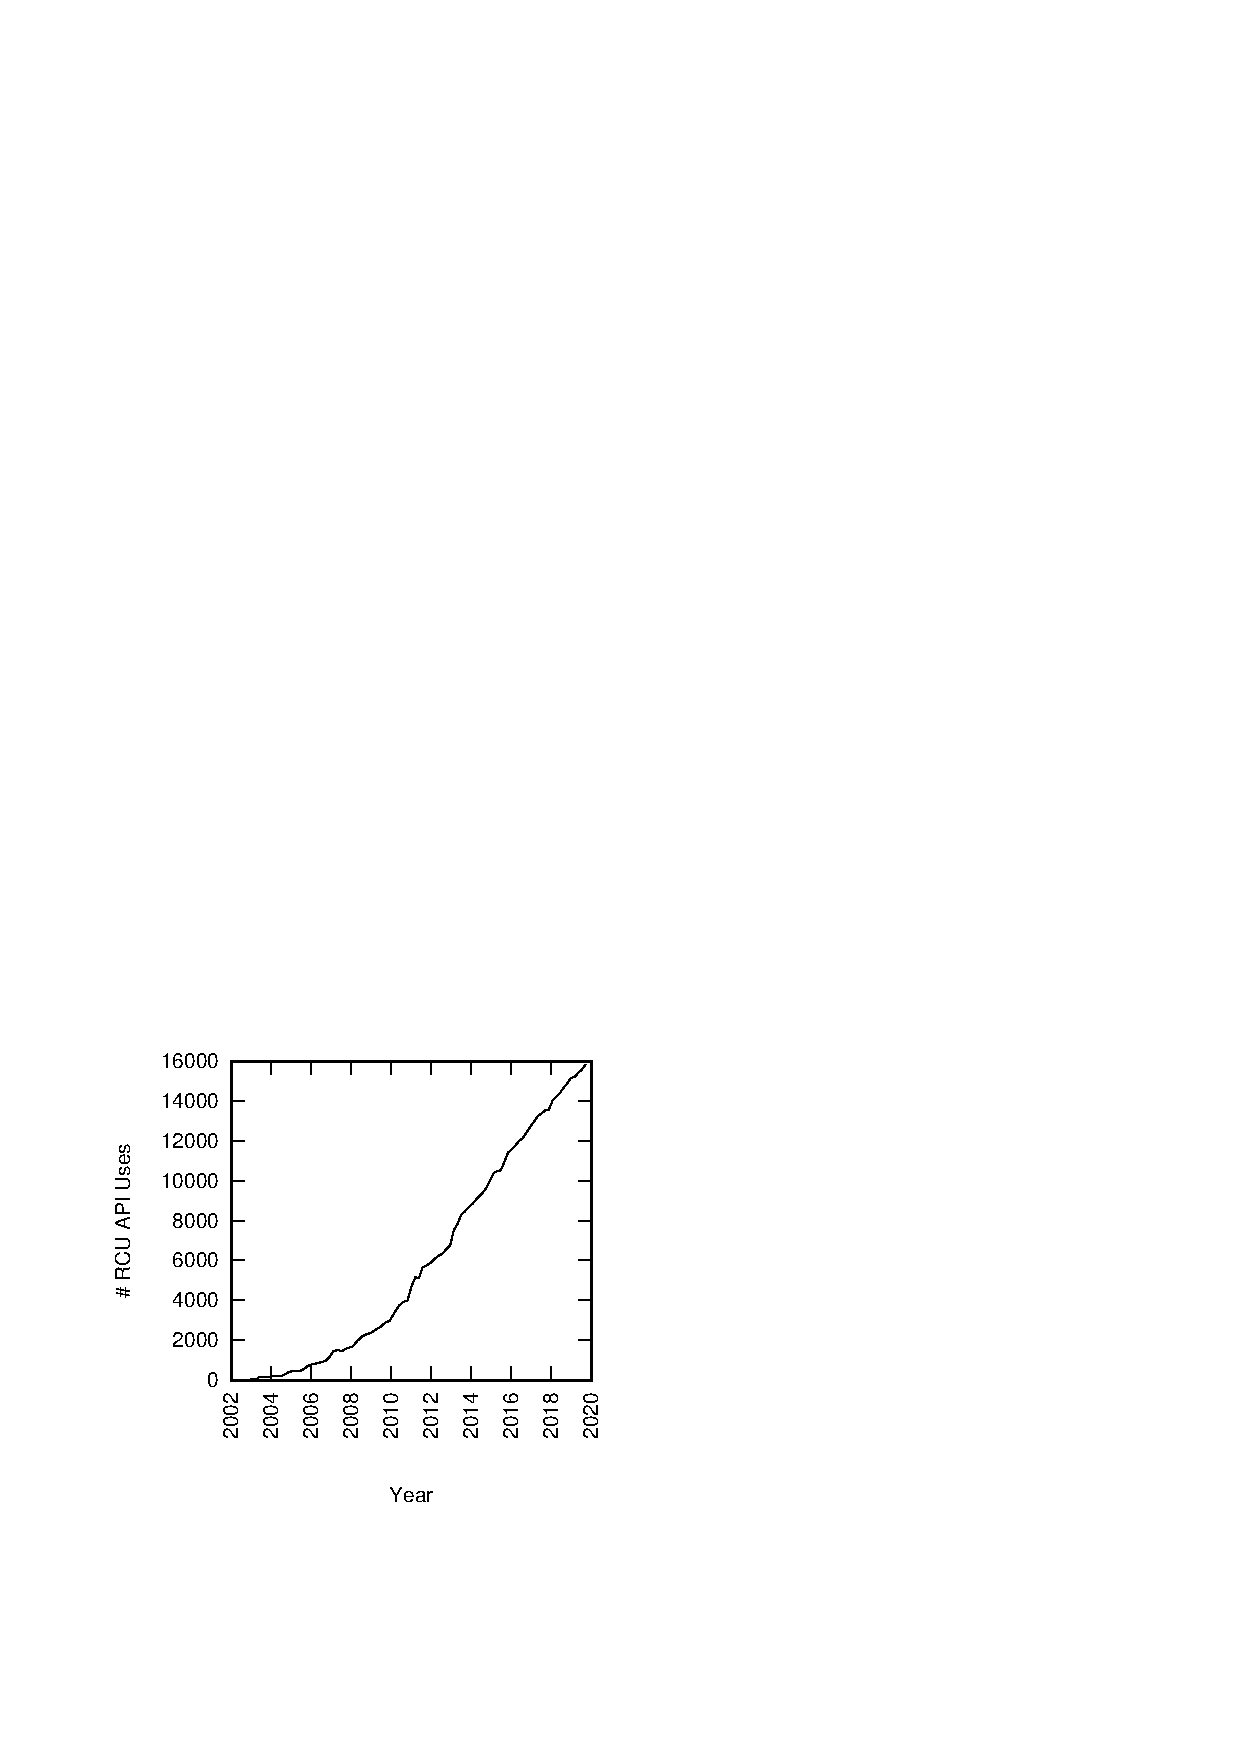
\includegraphics{defer/linux-RCU}}
\caption{RCU Usage in the Linux Kernel}
\label{fig:defer:RCU Usage in the Linux Kernel}
\end{figure}

RCU has been used in the Linux kernel since
October 2002~\cite{Torvalds2.5.43}.
Use of the RCU API has increased substantially since that time,
as can be seen in
Figure~\ref{fig:defer:RCU Usage in the Linux Kernel}.
In fact, code very similar to that in
Listing~\ref{lst:defer:Insertion and Deletion With Concurrent Readers}
is used in the Linux kernel.
RCU has enjoyed heavy use both prior to and since its acceptance
in the Linux kernel, as discussed in
\cref{sec:defer:RCU Related Work}.

It is therefore safe to say that RCU enjoys wide practical applicability.

The minimal example discussed in this section is a good introduction to RCU\@.
However, effective use of RCU often requires that you think differently
about your problem.
It is therefore useful to examine RCU's fundamentals, a task taken up
by the following section.

% defer/rcufundamental.tex

\subsection{RCU Fundamentals}
\label{sec:defer:RCU Fundamentals}
\OriginallyPublished{Section}{sec:defer:RCU Fundamentals}{RCU Fundamentals}{Linux Weekly News}{PaulEMcKenney2007WhatIsRCUFundamentally}

Authors: Paul E. McKenney and Jonathan Walpole

Read-copy update (RCU) 는 2002년 10월에 리눅스 커널에 추가된, 하나의 동기화
메커니즘입니다.
RCU 는 읽기 작업들이 업데이트 작업들과 동시에 일어날 수 있도록 함으로써 확장성
개선을 달성합니다.
기존에 일반적으로 사용되어온, 동시에 수행되는 쓰레드들에 대해 그것들이 읽기를
하는지 업데이트를 하는지와 상관없이 상호 배제를 보장하는 락킹 기능들 또는
동시의 읽기 작업은 허용하지만 업데이트가 함께 수행되는 것은 막는 reader-writer
락들과는 대조적으로 RCU 는 하나의 업데이트 쓰레드와 여러 읽기 쓰레드들 사이의
동시성을 지원합니다.
RCU 는 오브젝트들의 여러 버전들을 유지하고 그것들이 이전부터 존재해온 모든
읽기쪽 크리티컬 섹션들이 완료되기 전까지는 메모리에서 해제하지 않음으로써 읽기
작업들이 일관적임을 보장합니다.
RCU 는 오브젝트의 새 버전을 공개하고 읽는데, 그리고 예전 버전들의 정리 작업을
뒤로 미루어 한번에 처리하는데에 효과적이고 확장성 있는 메커니즘을 정의하고
사용합니다.
이런 메커니즘들은 작업을 읽기와 업데이트쪽 수행경로로 분산시키되 읽기 쪽
수행경로가 극단적으로 빠르게 하는데에 해저드 포인터와 유사한 복사와 규칙 완화를
골자로 하는 최적화 기술을 사용하지만, 읽기 쪽의 재시도는 필요 없게 합니다.
일부 경우에는 (CPU 를 뺏기지 않는 커널들), RCU 의 읽기 쪽 기능들은 아예
오버헤드가 없습니다.
\iffalse

Read-copy update (RCU) is a synchronization mechanism that was added to
the Linux kernel in October of 2002.
RCU achieves scalability
improvements by allowing reads to occur concurrently with updates.
In contrast with conventional locking primitives that ensure mutual exclusion
among concurrent threads regardless of whether they be readers or
updaters, or with reader-writer locks that allow concurrent reads but not in
the presence of updates, RCU supports concurrency between a single
updater and multiple readers.
RCU ensures that reads are coherent by
maintaining multiple versions of objects and ensuring that they are not
freed up until all pre-existing read-side critical sections complete.
RCU defines and uses efficient and scalable mechanisms for publishing
and reading new versions of an object, and also for deferring the collection
of old versions.
These mechanisms distribute the work among read and
update paths in such a way as to make read paths extremely fast, using
replication and weakening optimizations in a manner similar to
hazard pointers, but without the need for read-side retries.
In some cases (non-preemptible kernels), RCU's read-side primitives have
zero overhead.
\fi

\QuickQuiz{}
	하지만 Section~\ref{sec:defer:Sequence Locks} 의 시퀀스 락 역시 읽기
	쓰레드들과 업데이트 쓰레드들이 동시에 일을 할 수 있도록 하지 않던가요?
	\iffalse

	But doesn't Section~\ref{sec:defer:Sequence Locks}'s seqlock
	also permit readers and updaters to get work done concurrently?
	\fi
\QuickQuizAnswer{
	맞는 말이고 아닌 말이기도 합니다.
	시퀀스 락의 읽기 쓰레드들은 쓰기 쓰레드들과 동시에 수행될 수 있지만,
	이런 상황이 발생할 때마다, {\tt read\_seqretry()} 기능이 읽기 쓰레드는
	다시 수행을 시도하도록 강제할 겁니다.
	이는 시퀀스 락을 사용하명 업데이트 쓰레드와 동시에 수행되는 읽기
	쓰레드가 하는 일은 모두 취소되고 다시 수행될 것을 의미합니다.
	따라서 시퀀스 락을 사용하는 읽기 작업은 업데이트 작업과 동시에
	\emph{수행} 될 수 있지만, 이런 경우에 실제로는 어떤 일도 만들어내지
	못합니다.

	반면에, RCU 읽기 쓰레드들은 동시에 RCU 업데이트 쓰레드들이 존재하더라도
	의미있는 일을 처리해낼 수 있습니다.
	\iffalse

	Yes and no.
	Although seqlock readers can run concurrently with
	seqlock writers, whenever this happens, the {\tt read\_seqretry()}
	primitive will force the reader to retry.
	This means that any work done by a seqlock reader running concurrently
	with a seqlock updater will be discarded and redone.
	So seqlock readers can \emph{run} concurrently with updaters,
	but they cannot actually get any work done in this case.

	In contrast, RCU readers can perform useful work even in presence
	of concurrent RCU updaters.
	\fi
} \QuickQuizEnd

이는 ``RCU 는 정확히 무엇인가?'' 하는 질문과, 아마도 ``RCU 는 어떻게 동작할 수
\emph{있는가}?'' 하는 질문을 이끌어낼 수 있을 겁니다 (또는, 드물지 않게, RCU 는
동작할 수 없을 것이라는 단정을).
이 문서는 이런 질문들을 기본적 관점에서부터 다룹니다; 뒤의 일부는 RCU 를
사용법과 API 관점에서 살펴봅니다.
마지막 부분은 또한 참고할 문서 목록을 포함합니다.

RCU 는 세개의 기본적 메커니즘으로 만들어지는데, 첫번째는 항목 삽입에 사용되고,
두번째 것은 항목 삭제에, 그리고 세번째 것은 읽기 쓰레드들이 동시의 항목 추가와
삭제에 문제 없이 동작하도록 하는데 사용됩니다.
Section~\ref{sec:defer:Publish-Subscribe Mechanism}
은 항목 추가를 위한 publish-subscribe 메커니즘을 설명하고,
Section~\ref{sec:defer:Wait For Pre-Existing RCU Readers to Complete}
에서는 먼저 시작된 RCU 읽기 쓰레드들을 어떻게 기다려서 항목 삭제가 가능하게
하는지 설명하며,
Section~\ref{sec:defer:Maintain Multiple Versions of Recently Updated Objects}
에서는 최근에 업데이트된 오브젝트들의 여러 버전들을 어떻게 관리해서 동시의 항목
추가와 삭제를 가능하게 하는지 설명합니다.
마지막으로,
Section~\ref{sec:defer:Summary of RCU Fundamentals}
에서는 RCU 기본사항을 요약합니다.
\iffalse

This leads to the question ``what exactly is RCU?'', and perhaps also
to the question ``how can RCU \emph{possibly} work?'' (or, not
infrequently, the assertion that RCU cannot possibly work).
This document addresses these questions from a fundamental viewpoint;
later installments look at them from usage and from API viewpoints.
This last installment also includes a list of references.

RCU is made up of three fundamental mechanisms, the first being
used for insertion, the second being used for deletion, and the third
being used to allow readers to tolerate concurrent insertions and deletions.
Section~\ref{sec:defer:Publish-Subscribe Mechanism}
describes the publish-subscribe mechanism used for insertion,
Section~\ref{sec:defer:Wait For Pre-Existing RCU Readers to Complete}
describes how waiting for pre-existing RCU readers enabled deletion,
and
Section~\ref{sec:defer:Maintain Multiple Versions of Recently Updated Objects}
discusses how maintaining multiple versions of recently updated objects
permits concurrent insertions and deletions.
Finally,
Section~\ref{sec:defer:Summary of RCU Fundamentals}
summarizes RCU fundamentals.
\fi

\subsubsection{Publish-Subscribe Mechanism}
\label{sec:defer:Publish-Subscribe Mechanism}

\begin{figure}[tbp]
{ \scriptsize
\begin{verbatim}
  1 struct foo {
  2   int a;
  3   int b;
  4   int c;
  5 };
  6 struct foo *gp = NULL;
  7
  8 /* . . . */
  9
 10 p = kmalloc(sizeof(*p), GFP_KERNEL);
 11 p->a = 1;
 12 p->b = 2;
 13 p->c = 3;
 14 gp = p;
\end{verbatim}
}
\caption{Data Structure Publication (Unsafe)}
\label{fig:defer:Data Structure Publication (Unsafe)}
\end{figure}

RCU 의 핵심 요소 중 하나는 데이터가 동시에 수정되고 있는데도 불구하고 안전하게
그 데이터를 읽을 수 있는 능력입니다.
동시의 항목 삽입에 이런 능력을 제공하기 위해, RCU 는 공개-구독
(publish-subscribe) 메커니즘이라 생각될 수 있는 방법을 상요합니다.
예를 들어, 초기에 \co{NULL} 인 전역 포인터 \co{gp} 가 새로 할당되고 초기화된
데이터 구조체로의 포인터로 수정되려 한다고 생각해 봅시다.
Figure~\ref{fig:defer:Data Structure Publication (Unsafe)} 에 보이는 코드 조각
(추가로 적절한 락킹을 포함해서) 이 이 목적으로 사용될 수 있을 것입니다.
\iffalse

One key attribute of RCU is the ability to safely scan data, even
though that data is being modified concurrently.
To provide this ability for concurrent insertion,
RCU uses what can be thought of as a publish-subscribe mechanism.
For example, consider an initially \co{NULL} global pointer
\co{gp} that is to be modified to point to a newly allocated
and initialized data structure.
The code fragment shown in
Figure~\ref{fig:defer:Data Structure Publication (Unsafe)}
(with the addition of appropriate locking)
might be used for this purpose.
\fi

안타깝게도, 컴파일러와 CPU 가 마지막 네개의 할당문이 순서대로 수행하도록
강제하는 것이 전혀 없습니다.
\co{gp} 로의 할당이 \co{p} 필드들의 초기화 전에 일어난다면, 동시 수행중인 읽기
작업들은 이 초기화되지 않은 값들을 볼 수 있을 겁니다.
이것들이 순서를 지키도록 하기 위해 메모리 배리어들이 필요합니다만, 메모리
배리어들은 사용하기가 어렵기로 악명높습니다.
따라서 그것들을 공개 의미를 갖는 \co{rcu_assign_pointer()} 기능에 집어넣습니다.
그렇게 되면 마지막 네줄은 다음과 같이 될겁니다:
\iffalse

Unfortunately, there is nothing forcing the compiler and CPU to execute
the last four assignment statements in order.
If the assignment to \co{gp} happens before the initialization
of \co{p} fields, then concurrent readers could see the
uninitialized values.
Memory barriers are required to keep things ordered, but memory barriers
are notoriously difficult to use.
We therefore encapsulate them into a primitive
\co{rcu_assign_pointer()} that has publication semantics.
The last four lines would then be as follows:
\fi

\vspace{5pt}
\begin{minipage}[t]{\columnwidth}
\scriptsize
\begin{verbatim}
  1 p->a = 1;
  2 p->b = 2;
  3 p->c = 3;
  4 rcu_assign_pointer(gp, p);
\end{verbatim}
\end{minipage}
\vspace{5pt}

이 \co{rcu_assign_pointer()} 는 새 구조체를 \emph{공개}하고, 컴파일러와 CPU 가
\co{gp} 로의 할당이 \co{p} 로 참조되는 필드들의 할당 \emph{후에} 수행하도록
강제할 겁니다.

하지만, 업데이트 작업에 순서를 맞추는 것만으로는 충분치 않은데, 읽기 작업도
적절하게 순서가 맞춰져야 하기 때문입니다.
다음과 같은 코드 조각의 예를 생각해 봅시다:
\iffalse

The \co{rcu_assign_pointer()}
would \emph{publish} the new structure, forcing both the compiler
and the CPU to execute the assignment to \co{gp} \emph{after}
the assignments to the fields referenced by \co{p}.

However, it is not sufficient to only enforce ordering at the
updater, as the reader must enforce proper ordering as well.
Consider for example the following code fragment:
\fi

\vspace{5pt}
\begin{minipage}[t]{\columnwidth}
\scriptsize
\begin{verbatim}
  1 p = gp;
  2 if (p != NULL) {
  3   do_something_with(p->a, p->b, p->c);
  4 }
\end{verbatim}
\end{minipage}
\vspace{5pt}

이 코드 조각은 잘못된 순서에 문제가 없을 것처럼 보이지만, 안타깝게도 DEC Alpha
CPU~\cite{PaulMcKenney2005i,PaulMcKenney2005j} 와 값을 예측하는 컴파일러
최적화는, 믿든 안믿든, \co{p->a}, \co{p->b}, 그리고 \co{p->c} 가 \co{p} 의 값
전에 메모리로부터 가져와질 수 있게 할 수 있습니다.
이런 현상은 컴파일러가 \co{p} 의 값을 추측하고 \co{p->a}, \co{p->b}, 그리고
\co{p->c} 값을 가져온 후에 그 추측이 맞았는지 보기 위해 \co{p} 의 실제 값을
가져오는, 컴파일러의 값 추측 최적화의 경우에서 보기가 가장 쉬울 겁니다.
이런 종류의 최적화는 상당히 공격적이고 미친 행위 같지만, 프로파일 기반의
최적화의 문맥에서는 실제로 일어나는 일입니다.
\iffalse

Although this code fragment might well seem immune to misordering,
unfortunately, the
DEC Alpha CPU~\cite{PaulMcKenney2005i,PaulMcKenney2005j}
and value-speculation compiler optimizations can, believe it or not,
cause the values of \co{p->a}, \co{p->b}, and
\co{p->c} to be fetched before the value of \co{p}.
This is perhaps easiest to see in the case of value-speculation
compiler optimizations, where the compiler guesses the value
of \co{p} fetches \co{p->a}, \co{p->b}, and
\co{p->c} then fetches the actual value of \co{p}
in order to check whether its guess was correct.
This sort of optimization is quite aggressive, perhaps insanely so,
but does actually occur in the context of profile-driven optimization.
\fi

분명히, 우리는 컴파일러와 CPU 로부터 이런 종류의 야바위질을 막아야 합니다.
\co{rcu_dereference()} 기능은 이런 목적을 위해 필요한 어떤 메모리 배리어
인스트럭션과 컴파일러 지시어들을 사용합니다:\footnote{
	리눅스 커널에서, \co{rcu_dereference()} 는 volatile 캐스팅으로
	구현되고, DEC Alpha 에서는 메모리 배리어 인스트럭션으로 구현됩니다.
	C11 과 C++11 표준에서는 \co{memory_order_consume} 이
	\co{rcu_dereference()} 지원을 제공하기 위한 의도로 만들어졌습니다만,
	이를 native로 구현한 컴파일러는 아직 없습니다.
	(컴파일러들은 대신 \co{memory_order_consume} 을
	\co{memory_order_acuire} 로 강화시켜서, 약한 순서 규칙의 시스템에서는
	필요없는 메모리 배리어 인스트럭션을 만듭니다.)}
\iffalse

Clearly, we need to prevent this sort of skullduggery on the
part of both the compiler and the CPU.
The \co{rcu_dereference()} primitive uses
whatever memory-barrier instructions and compiler
directives are required for this purpose:\footnote{
	In the Linux kernel, \co{rcu_dereference()} is implemented via
	a volatile cast, and, on DEC Alpha, a memory barrier instruction.
	In the C11 and C++11 standards, \co{memory_order_consume}
	is intended to provide longer-term support for \co{rcu_dereference()},
	but no compilers implement this natively yet.
	(They instead strengthen \co{memory_order_consume} to
	\co{memory_order_acquire}, thus emitting a needless memory-barrier
	instruction on weakly ordered systems.)}
\fi

\vspace{5pt}
\begin{minipage}[t]{\columnwidth}
\scriptsize
\begin{verbatim}
  1 rcu_read_lock();
  2 p = rcu_dereference(gp);
  3 if (p != NULL) {
  4   do_something_with(p->a, p->b, p->c);
  5 }
  6 rcu_read_unlock();
\end{verbatim}
\end{minipage}
\vspace{5pt}

따라서 \co{rcu_dereference()} 함수는 특정 포인터로 주어지는 값에 대한
\emph{구독} 으로, 뒤따르는 dereference 오퍼레이션들은 해당 포인터를 공개한,
연관된 \co{rcu_assign_pointer()} 오퍼레이션 전에 발생한 초기화 작업의 결과들을
보게 될 것이 보장된다고 이해될 수 있습니다.
\co{rcu_read_lock()} 과 \co{rcu_read_unlock()} 함수 호출들은 반드시 필요합니다:
이것들은 RCU read-side 크리티컬 섹션을 정의합니다.
이것들의 목적인
Section~\ref{sec:defer:Wait For Pre-Existing RCU Readers to Complete} 에서
설명됩니다만, 이것들은 결코 스피닝하거나 블락킹 하지 않고, \co{list_add_rcu()}
가 동시에 수행되는 것을 막지도 않습니다.
사실, \co{CONFIG_PREEMPT} 옵션이 켜져있지 않은 커널에서 이것들은 아무 코드도
생성하지 않습니다.
\iffalse

The \co{rcu_dereference()} primitive can thus be thought of
as \emph{subscribing} to a given value of the specified pointer,
guaranteeing that subsequent dereference operations will see any
initialization that occurred before the corresponding
\co{rcu_assign_pointer()} operation that published that pointer.
The \co{rcu_read_lock()} and \co{rcu_read_unlock()}
calls are absolutely required: they define the extent of the
RCU read-side critical section.
Their purpose is explained in
Section~\ref{sec:defer:Wait For Pre-Existing RCU Readers to Complete},
however, they never spin or block, nor do they prevent the
\co{list_add_rcu()} from executing concurrently.
In fact, in non-\co{CONFIG_PREEMPT} kernels, they generate
absolutely no code.
\fi

\begin{figure}[tb]
\begin{center}
\resizebox{3in}{!}{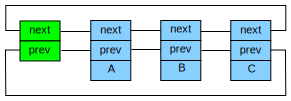
\includegraphics{defer/Linux_list}}
\end{center}
\caption{Linux Circular Linked List}
\label{fig:defer:Linux Circular Linked List}
\end{figure}

\begin{figure}[tb]
\begin{center}
\resizebox{3in}{!}{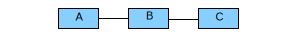
\includegraphics{defer/Linux_list_abbr}}
\end{center}
\caption{Linux Linked List Abbreviated}
\label{fig:defer:Linux Linked List Abbreviated}
\end{figure}

이론상으로는 \co{rcu_assign_pointer()} 와 \co{rcu_dereference()} 는 상상할 수
있는 RCU 로 보호되는 데이터 구조는 얼마든지 만들 수 있지만, 실제로는
고차원의 방법을 사용하는게 나은 경우가 많이 있습니다.
그런 이유로, \co{rcu_assign_pointer()} 와 \co{rcu_dereference()} 함수들이
리눅스에 있는 리스트 조정 API 의 특별한 RCU 사용 버전에 내장되어 있습니다.
리눅스는 이중 링크드 리스트의 두가지 버전을 가지고 있는데, 순환 형태의 {\tt
struct list\_head} 와 선형의 {\tt struct hlist\_head}/{\tt struct hlist\_node}
쌍입니다.
앞의 버전은
Figure~\ref{fig:defer:Linux Circular Linked List} 에 그려져 있는데, (왼쪽의)
초록 상자는 리스트 헤더를 나타내고 (오른쪽의 세개의) 파란 박스들은 리스트의
원소들을 의미합니다.
이 방법은 다루기가 힘들기 때문에
Figure~\ref{fig:defer:Linux Linked List Abbreviated} 에 보인 것처럼 헤더 없이
(파란) 원소들만을 보이는 형태로 간략화해서 나타낼 수 있습니다.
\iffalse

Although \co{rcu_assign_pointer()} and
\co{rcu_dereference()} can in theory be used to construct any
conceivable RCU-protected data structure, in practice it is often better
to use higher-level constructs.
Therefore, the \co{rcu_assign_pointer()} and
\co{rcu_dereference()}
primitives have been embedded in special RCU variants of Linux's
list-manipulation API.
Linux has two variants of doubly linked list, the circular
{\tt struct list\_head} and the linear
{\tt struct hlist\_head}/{\tt struct hlist\_node} pair.
The former is laid out as shown in
Figure~\ref{fig:defer:Linux Circular Linked List},
where the green (leftmost) boxes represent the list header and the blue
(rightmost three) boxes represent the elements in the list.
This notation is cumbersome, and will therefore be abbreviated as shown in
Figure~\ref{fig:defer:Linux Linked List Abbreviated},
which shows only the non-header (blue) elements.
\fi

\begin{figure}[tbp]
{ \scriptsize
\begin{verbatim}
  1 struct foo {
  2   struct list_head *list;
  3   int a;
  4   int b;
  5   int c;
  6 };
  7 LIST_HEAD(head);
  8
  9 /* . . . */
 10
 11 p = kmalloc(sizeof(*p), GFP_KERNEL);
 12 p->a = 1;
 13 p->b = 2;
 14 p->c = 3;
 15 list_add_rcu(&p->list, &head);
\end{verbatim}
}
\caption{RCU Data Structure Publication}
\label{fig:defer:RCU Data Structure Publication}
\end{figure}

이 링크드 리스트에 포인터 공개 예제의 기법을 적용하는 것은
Figure~\ref{fig:defer:RCU Data Structure Publication} 에 보여진 코드와 같은
형태로 귀결될 겁니다.

Line~15 는 여러개의 \co{list_add_rcu()} 가 동시에 수행되는 것을 막기 위해 어떤
다른 동기화 메커니즘 (가장 흔하게는 어떤 종류의 락) 을 사용해야만 합니다.
하지만, 그런 동기화는 이 \co{list_add()} 의 수행을 RCU 읽기 작업들과 동시에
수행되는 것을 못하게 하지는 않습니다.

RCU 로 보호되는 리스트를 구독하는 행위는 간단합니다:
\iffalse

Adapting the pointer-publish example for the linked list results in
the code shown in
Figure~\ref{fig:defer:RCU Data Structure Publication}.

Line~15 must be protected by some synchronization mechanism (most
commonly some sort of lock) to prevent multiple \co{list_add_rcu()}
instances from executing concurrently.
However, such synchronization does not prevent this \co{list_add()}
instance from executing concurrently with RCU readers.

Subscribing to an RCU-protected list is straightforward:
\fi

\vspace{5pt}
\begin{minipage}[t]{\columnwidth}
\scriptsize
\begin{verbatim}
  1 rcu_read_lock();
  2 list_for_each_entry_rcu(p, head, list) {
  3   do_something_with(p->a, p->b, p->c);
  4 }
  5 rcu_read_unlock();
\end{verbatim}
\end{minipage}
\vspace{5pt}

앞의 \co{list_add_rcu()} 함수는 원소를 공개하고, 특정 리스트의 헤드에 집어넣고,
이에 연관된 \co{list_for_each_entry_rcu()} 호출이 정상적으로 같은 원소를
구독하게 될것을 보장합니다.
\iffalse

The \co{list_add_rcu()} primitive publishes an entry, inserting it at
the head of the specified list, guaranteeing that the corresponding
\co{list_for_each_entry_rcu()} invocation will properly subscribe to
this same entry.
\fi

\QuickQuiz{}
	{\tt list\_add\_rcu()} 와 정확히 똑같은 시간에
	{\tt list\_for\_each\_entry\_rcu()} 이 수행되면 segfault 가 날 수 있을
	것 같은데, 이걸 무엇이 방지해 주나요?
	\iffalse

	What prevents the {\tt list\_for\_each\_entry\_rcu()} from
	getting a segfault if it happens to execute at exactly the same
	time as the {\tt list\_add\_rcu()}?
	\fi
\QuickQuizAnswer{
	리눅스가 돌아가는 모든 시스템에서 포인터로의 로드와 스토어는 모두
	어토믹한데, 즉, 포인터로의 스토어가 같은 포인터로부터의 로드와 같은
	시점에 일어난다면, 이 로드는 초기값이나 저장된 값을 가져오지, 그 두
	값이 섞여진 값을 가져오는 일은 결코 없습니다.
	또한, {\tt list\_for\_each\_entry\_rcu()} 는 항상 리스트를 앞으로만
	움직이지, 결코 뒤로 움직이지는 않습니다.
	따라서, {\tt list\_for\_each\_entry\_rcu()} 는 {\tt list\_add\_rc()} 를
	통해 들어온 원소를 보거나 보지 않을 뿐이지만 어떤 경우든 적합하게 잘
	형성된 리스트를 볼 겁니다.
	\iffalse

	On all systems running Linux, loads from and stores
	to pointers are atomic, that is, if a store to a pointer occurs at
	the same time as a load from that same pointer, the load will return
	either the initial value or the value stored, never some bitwise
	mashup of the two.
	In addition, the {\tt list\_for\_each\_entry\_rcu()} always proceeds
	forward through the list, never looking back.
	Therefore, the {\tt list\_for\_each\_entry\_rcu()} will either see
	the element being added by {\tt list\_add\_rcu()} or it will not,
	but either way, it will see a valid well-formed list.
	\fi
} \QuickQuizEnd

\begin{figure}[tb]
\begin{center}
\resizebox{3in}{!}{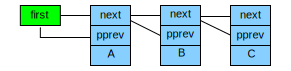
\includegraphics{defer/Linux_hlist}}
\end{center}
\caption{Linux Linear Linked List}
\label{fig:defer:Linux Linear Linked List}
\end{figure}

리눅스의 다른 이중 링크드 리스트인 hlist 는 선형 리스트인데, 이는 헤더로의
포인터만이 필요하지
Figure~\ref{fig:defer:Linux Linear Linked List} 에 보여진 순환 형태의
리스트처럼 두개의 포인터가 필요하진 않습니다.
따라서, hlist 의 사용은 해시 버킷 배열들이나 커다란 해시 테이블에서는 메모리
사용량을 반으로 줄일 수 있습니다.
앞에서와 같이, 이 형태는 다루기가 까다로우므로, hlist 들은
Figure~\ref{fig:defer:Linux Linked List Abbreviated} 에 보인 것과 같은 형태로
간략화 될 겁니다.
\iffalse

Linux's other doubly linked list, the hlist,
is a linear list, which means that
it needs only one pointer for the header rather than the two
required for the circular list, as shown in
Figure~\ref{fig:defer:Linux Linear Linked List}.
Thus, use of hlist can halve the memory consumption for the hash-bucket
arrays of large hash tables.
As before, this notation is cumbersome, so hlists will be abbreviated
in the same way lists are, as shown in
Figure~\ref{fig:defer:Linux Linked List Abbreviated}.
\fi

\begin{figure}[tbp]
{ \scriptsize
\begin{verbatim}
  1 struct foo {
  2   struct hlist_node *list;
  3   int a;
  4   int b;
  5   int c;
  6 };
  7 HLIST_HEAD(head);
  8
  9 /* . . . */
 10
 11 p = kmalloc(sizeof(*p), GFP_KERNEL);
 12 p->a = 1;
 13 p->b = 2;
 14 p->c = 3;
 15 hlist_add_head_rcu(&p->list, &head);
\end{verbatim}
}
\caption{RCU {\tt hlist} Publication}
\label{fig:defer:RCU hlist Publication}
\end{figure}

새로운 원소를 RCU 로 보호되는 hlist 에 공개하는 건
as shown in Figure~\ref{fig:defer:RCU hlist Publication} 에 보여진 것처럼,
순환형 리스트에서 했던 것과 상당히 유사합니다.

앞에서와 같이, line~15 는 예를 들면 락과 같은, 어떤 종류의 동기화 메커니즘으로
보호되어야만 합니다.

RCU 로 보호되는 hlist 를 구독하는 행위 역시 순환형 리스트에서와 비슷합니다:
\iffalse

Publishing a new element to an RCU-protected hlist is quite similar
to doing so for the circular list,
as shown in Figure~\ref{fig:defer:RCU hlist Publication}.

As before, line~15 must be protected by some sort of synchronization
mechanism, for example, a lock.

Subscribing to an RCU-protected hlist is also similar to the
circular list:
\fi

\vspace{5pt}
\begin{minipage}[t]{\columnwidth}
\scriptsize
\begin{verbatim}
  1 rcu_read_lock();
  2 hlist_for_each_entry_rcu(p, q, head, list) {
  3   do_something_with(p->a, p->b, p->c);
  4 }
  5 rcu_read_unlock();
\end{verbatim}
\end{minipage}
\vspace{5pt}

\QuickQuiz{}
	{\tt list\_for\_each\_entry\_rcu()} 에서는 한개면 되었던 포인터가 왜
	{\tt hlist\_for\_each\_entry\_rcu()} 에서는 두개나 넘겨줘야 하는거죠?
	\iffalse

	Why do we need to pass two pointers into
	{\tt hlist\_for\_each\_entry\_rcu()}
	when only one is needed for {\tt list\_for\_each\_entry\_rcu()}?
	\fi
\QuickQuizAnswer{
	hlist 에서는 헤드를 만나는 대신에 NULL 체크를 할 필요가 있기
	때문입니다.
	(하나의 포인터만 사용하는 {\tt hlist\_for\_each\_entry\_rcu()} 를
	한번 구현해 보세요.
	만약 좋은 해결책을 찾는다면, 정말 좋은 일일 겁니다!)
	\iffalse

	Because in an hlist it is necessary to check for
	NULL rather than for encountering the head.
	(Try coding up a single-pointer {\tt hlist\_for\_each\_entry\_rcu()}.
	If you come up with a nice solution, it would be a very good thing!)
	\fi
} \QuickQuizEnd

\begin{table*}[tb]
\begin{center}
\scriptsize
\begin{tabular}{l||l|l|l}
Category  & Publish	& Retract	& Subscribe \\
\hline
\hline
Pointers  & \co{rcu_assign_pointer()}
			& \co{rcu_assign_pointer(..., NULL)}~~
					& \co{rcu_dereference()} \\
\hline
Lists     & \parbox{1.5in}{
		\co{list_add_rcu()} \\
		\co{list_add_tail_rcu()} \\
		\co{list_replace_rcu()} }
			& \co{list_del_rcu()}
					& \co{list_for_each_entry_rcu()}~~~ \\
\hline
Hlists    & \parbox{1.5in}{
		\co{hlist_add_after_rcu()} \\
		\co{hlist_add_before_rcu()}  \\
		\co{hlist_add_head_rcu()} \\
		\co{hlist_replace_rcu()} }
			& \co{hlist_del_rcu()}
					& \co{hlist_for_each_entry_rcu()}~~~~~
\end{tabular}
\end{center}
\caption{RCU Publish and Subscribe Primitives}
\label{tab:defer:RCU Publish and Subscribe Primitives}
\end{table*}

RCU 공개와 구독 기능들의 집합이
Table~\ref{tab:defer:RCU Publish and Subscribe Primitives} 에 ``구독취소'' 또는
철회를 위한 추가적인 기능들과 함께 표시 되어 있습니다.

\co{list_replace_rcu()}, \co{list_del_rcu()},
\co{hlist_replace_rcu()}, and \co{hlist_del_rcu()}
API 들이 복잡도를 더함을 알아두세요.
교체되거나 삭제된 데이터 원소를 메모리에서 해제하는데 안전한 시점은 언제일까요?
자세히 들어가서, 모든 읽기 작업들이 특정 데이터 원소로의 레퍼런스들을
해제한 시점을 어떻게 하면 알 수 있을까요?

이 질문들은 다음의 섹션에서 다루어집니다.
\iffalse

The set of RCU publish and subscribe primitives are shown in
Table~\ref{tab:defer:RCU Publish and Subscribe Primitives},
along with additional primitives to ``unpublish'', or retract.

Note that the \co{list_replace_rcu()}, \co{list_del_rcu()},
\co{hlist_replace_rcu()}, and \co{hlist_del_rcu()}
APIs add a complication.
When is it safe to free up the data element that was replaced or
removed?
In particular, how can we possibly know when all the readers
have released their references to that data element?

These questions are addressed in the following section.
\fi

\subsubsection{Wait For Pre-Existing RCU Readers to Complete}
\label{sec:defer:Wait For Pre-Existing RCU Readers to Complete}

In its most basic form, RCU is a way of waiting for things to finish.
Of course, there are a great many other ways of waiting for things to
finish, including reference counts, reader-writer locks, events, and so on.
The great advantage of RCU is that it can wait for each of
(say) 20,000 different things without having to explicitly
track each and every one of them, and without having to worry about
the performance degradation, scalability limitations, complex deadlock
scenarios, and memory-leak hazards that are inherent in schemes
using explicit tracking.

In RCU's case, the things waited on are called
``RCU read-side critical sections''.
An RCU read-side critical section starts with an
\co{rcu_read_lock()} primitive, and ends with a corresponding
\co{rcu_read_unlock()} primitive.
RCU read-side critical sections can be nested, and may contain pretty
much any code, as long as that code does not explicitly block or sleep
(although a special form of RCU called SRCU~\cite{PaulEMcKenney2006c}
does permit general sleeping in SRCU read-side critical sections).
If you abide by these conventions, you can use RCU to wait for \emph{any}
desired piece of code to complete.

RCU accomplishes this feat by indirectly determining when these
other things have finished~\cite{PaulEMcKenney2007whatisRCU,
PaulEMcKenney2007PreemptibleRCU}.

\begin{figure}[tb]
\begin{center}
\resizebox{3in}{!}{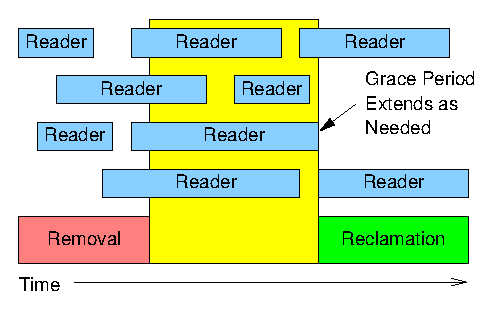
\includegraphics{defer/GracePeriodGood}}
\end{center}
\caption{Readers and RCU Grace Period}
\label{fig:defer:Readers and RCU Grace Period}
\end{figure}

In particular, as shown in
Figure~\ref{fig:defer:Readers and RCU Grace Period},
RCU is a way of
waiting for pre-existing RCU read-side critical sections to completely
finish, including memory operations executed by those critical sections.
However, note that RCU read-side critical sections
that begin after the beginning
of a given grace period can and will extend beyond the end of that grace
period.

The following pseudocode shows the basic form of algorithms that use
RCU to wait for readers:

\begin{enumerate}
\item	Make a change, for example, replace an element in a linked list.
\item	Wait for all pre-existing RCU read-side critical sections to
	completely finish (for example, by using the
	\co{synchronize_rcu()} primitive).
	The key observation here is that subsequent RCU read-side critical
	sections have no way to gain a reference to the newly removed
	element.
\item	Clean up, for example, free the element that was replaced above.
\end{enumerate}

\begin{figure}[tbp]
{ \scriptsize
\begin{verbatim}
  1 struct foo {
  2   struct list_head *list;
  3   int a;
  4   int b;
  5   int c;
  6 };
  7 LIST_HEAD(head);
  8
  9 /* . . . */
 10
 11 p = search(head, key);
 12 if (p == NULL) {
 13   /* Take appropriate action, unlock, & return. */
 14 }
 15 q = kmalloc(sizeof(*p), GFP_KERNEL);
 16 *q = *p;
 17 q->b = 2;
 18 q->c = 3;
 19 list_replace_rcu(&p->list, &q->list);
 20 synchronize_rcu();
 21 kfree(p);
\end{verbatim}
}
\caption{Canonical RCU Replacement Example}
\label{fig:defer:Canonical RCU Replacement Example}
\end{figure}

The code fragment shown in
Figure~\ref{fig:defer:Canonical RCU Replacement Example},
adapted from those in Section~\ref{sec:defer:Publish-Subscribe Mechanism},
demonstrates this process, with field \co{a} being the search key.

Lines~19, 20, and 21 implement the three steps called out above.
Lines~16-19 gives RCU (``read-copy update'') its name: while permitting
concurrent \emph{reads}, line~16 \emph{copies} and lines~17-19
do an \emph{update}.

As discussed in Section~\ref{sec:defer:Introduction to RCU},
the \co{synchronize_rcu()} primitive can be quite simple
(see Section~\ref{sec:defer:``Toy'' RCU Implementations}
for additional ``toy'' RCU implementations).
However, production-quality implementations must deal with
difficult corner cases and also incorporate
powerful optimizations, both of which result in significant complexity.
Although it is good to know that there is a simple conceptual
implementation of \co{synchronize_rcu()}, other questions remain.
For example, what exactly do RCU
readers see when traversing a concurrently updated list?
This question is addressed in the following section.

\subsubsection{Maintain Multiple Versions of Recently Updated Objects}
\label{sec:defer:Maintain Multiple Versions of Recently Updated Objects}

This section demonstrates how RCU maintains multiple versions of
lists to accommodate synchronization-free readers.
Two examples are presented showing how an element
that might be referenced by a given reader must remain intact
while that reader remains in its RCU read-side critical section.
The first example demonstrates deletion of a list element,
and the second example demonstrates replacement of an element.

\paragraph{Example 1: Maintaining Multiple Versions During Deletion}
\label{sec:defer:Example 1: Maintaining Multiple Versions During Deletion}

We can now revisit the deletion example from
Section~\ref{sec:defer:Introduction to RCU},
but now with the benefit of a firm understanding of the fundamental
concepts underlying RCU.
To begin this new version of the deletion example,
we will modify lines~11-21 in
Figure~\ref{fig:defer:Canonical RCU Replacement Example}
to read as follows:

\vspace{5pt}
\begin{minipage}[t]{\columnwidth}
\scriptsize
\begin{verbatim}
  1 p = search(head, key);
  2 if (p != NULL) {
  3   list_del_rcu(&p->list);
  4   synchronize_rcu();
  5   kfree(p);
  6 }
\end{verbatim}
\end{minipage}
\vspace{5pt}

\begin{figure}[tb]
\begin{center}
\resizebox{3in}{!}{\includegraphics{defer/RCUDeletion}}
\end{center}
\caption{RCU Deletion From Linked List}
\label{fig:defer:RCU Deletion From Linked List}
\end{figure}

This code will update the list as shown in
Figure~\ref{fig:defer:RCU Deletion From Linked List}.
The triples in each element represent the values of fields \co{a},
\co{b}, and \co{c}, respectively.
The red-shaded elements
indicate that RCU readers might be holding references to them,
so in the initial state at the top of the diagram, all elements
are shaded red.
Please note that
we have omitted the backwards pointers and the link from the tail
of the list to the head for clarity.

After the \co{list_del_rcu()} on
line~3 has completed, the \co{5,6,7}~element
has been removed from the list, as shown in the second row of
Figure~\ref{fig:defer:RCU Deletion From Linked List}.
Since readers do not synchronize directly with updaters,
readers might be concurrently scanning this list.
These concurrent readers might or might not see the newly removed element,
depending on timing.
However, readers that were delayed (e.g., due to interrupts, ECC memory
errors, or, in \co{CONFIG_PREEMPT_RT} kernels, preemption)
just after fetching a pointer to the newly removed element might
see the old version of the list for quite some time after the
removal.
Therefore, we now have two versions of the list, one with element
\co{5,6,7} and one without.
The \co{5,6,7}~element in the second row of the figure is now
shaded yellow, indicating
that old readers might still be referencing it, but that new
readers cannot obtain a reference to it.

Please note that readers are not permitted to maintain references to
element~\co{5,6,7} after exiting from their RCU read-side
critical sections.
Therefore,
once the \co{synchronize_rcu()} on
line~4 completes, so that all pre-existing readers are
guaranteed to have completed,
there can be no more readers referencing this
element, as indicated by its green shading on the third row of
Figure~\ref{fig:defer:RCU Deletion From Linked List}.
We are thus back to a single version of the list.

At this point, the \co{5,6,7}~element may safely be
freed, as shown on the final row of
Figure~\ref{fig:defer:RCU Deletion From Linked List}.
At this point, we have completed the deletion of
element~\co{5,6,7}.
The following section covers replacement.

\paragraph{Example 2: Maintaining Multiple Versions During Replacement}
\label{sec:defer:Example 2: Maintaining Multiple Versions During Replacement}

To start the replacement example,
here are the last few lines of the
example shown in
Figure~\ref{fig:defer:Canonical RCU Replacement Example}:

\vspace{5pt}
\begin{minipage}[t]{\columnwidth}
\scriptsize
\begin{verbatim}
  1 q = kmalloc(sizeof(*p), GFP_KERNEL);
  2 *q = *p;
  3 q->b = 2;
  4 q->c = 3;
  5 list_replace_rcu(&p->list, &q->list);
  6 synchronize_rcu();
  7 kfree(p);
\end{verbatim}
\end{minipage}
\vspace{5pt}

\begin{figure}[tbp]
\begin{center}
\resizebox{2.7in}{!}{\includegraphics{defer/RCUReplacement}}
\end{center}
\caption{RCU Replacement in Linked List}
\label{fig:defer:RCU Replacement in Linked List}
\end{figure}

The initial state of the list, including the pointer \co{p},
is the same as for the deletion example, as shown on the
first row of
Figure~\ref{fig:defer:RCU Replacement in Linked List}.

As before,
the triples in each element represent the values of fields \co{a},
\co{b}, and \co{c}, respectively.
The red-shaded elements might be referenced by readers,
and because readers do not synchronize directly with updaters,
readers might run concurrently with this entire replacement process.
Please note that
we again omit the backwards pointers and the link from the tail
of the list to the head for clarity.

The following text describes how to replace the \co{5,6,7} element
with \co{5,2,3} in such a way that any given reader sees one of these
two values.

Line~1 \co{kmalloc()}s a replacement element, as follows,
resulting in the state as shown in the second row of
Figure~\ref{fig:defer:RCU Replacement in Linked List}.
At this point, no reader can hold a reference to the newly allocated
element (as indicated by its green shading), and it is uninitialized
(as indicated by the question marks).

Line~2 copies the old element to the new one, resulting in the
state as shown in the third row of
Figure~\ref{fig:defer:RCU Replacement in Linked List}.
The newly allocated element still cannot be referenced by readers, but
it is now initialized.

Line~3 updates \co{q->b} to the value ``2'', and
line~4 updates \co{q->c} to the value ``3'', as shown on the fourth row of
Figure~\ref{fig:defer:RCU Replacement in Linked List}.

Now, line~5 does the replacement, so that the new element is
finally visible to readers, and hence is shaded red, as shown on
the fifth row of
Figure~\ref{fig:defer:RCU Replacement in Linked List}.
At this point, as shown below, we have two versions of the list.
Pre-existing readers might see the \co{5,6,7} element (which is
therefore now shaded yellow), but
new readers will instead see the \co{5,2,3} element.
But any given reader is guaranteed to see some well-defined list.

After the \co{synchronize_rcu()} on line~6 returns,
a grace period will have elapsed, and so all reads that started before the
\co{list_replace_rcu()} will have completed.
In particular, any readers that might have been holding references
to the \co{5,6,7} element are guaranteed to have exited
their RCU read-side critical sections, and are thus prohibited from
continuing to hold a reference.
Therefore, there can no longer be any readers holding references
to the old element, as indicated its green shading in the sixth row of
Figure~\ref{fig:defer:RCU Replacement in Linked List}.
As far as the readers are concerned, we are back to having a single version
of the list, but with the new element in place of the old.

After the \co{kfree()} on line 7 completes, the list will
appear as shown on the final row of
Figure~\ref{fig:defer:RCU Replacement in Linked List}.

Despite the fact that RCU was named after the replacement case,
the vast majority of RCU usage within the Linux kernel relies on
the simple deletion case shown in
Section~\ref{sec:defer:Maintain Multiple Versions of Recently Updated Objects}.

\paragraph{Discussion}
\label{sec:defer:Discussion}

These examples assumed that a mutex was held across the entire
update operation, which would mean that there could be at most two
versions of the list active at a given time.

\QuickQuiz{}
	How would you modify the deletion example to permit more than two
	versions of the list to be active?
\QuickQuizAnswer{
	One way of accomplishing this is as shown in
	Figure~\ref{fig:defer:Concurrent RCU Deletion}.

\begin{figure}[htbp]
{ \centering
\begin{verbatim}
  1 spin_lock(&mylock);
  2 p = search(head, key);
  3 if (p == NULL)
  4   spin_unlock(&mylock);
  5 else {
  6   list_del_rcu(&p->list);
  7   spin_unlock(&mylock);
  8   synchronize_rcu();
  9   kfree(p);
 10 }
\end{verbatim}
}
\caption{Concurrent RCU Deletion}
\label{fig:defer:Concurrent RCU Deletion}
\end{figure}

	Note that this means that multiple concurrent deletions might be
	waiting in \co{synchronize_rcu()}.
} \QuickQuizEnd

\QuickQuiz{}
	How many RCU versions of a given list can be
	active at any given time?
\QuickQuizAnswer{
	That depends on the synchronization design.
	If a semaphore protecting the update is held across the grace period,
	then there can be at most two versions, the old and the new.

	However, suppose that only the search, the update, and the
	\co{list_replace_rcu()} were protected by a lock, so that
	the \co{synchronize_rcu()} was outside of that lock, similar
	to the code shown in
	Figure~\ref{fig:defer:Concurrent RCU Deletion}.
	Suppose further that a large number of threads undertook an
	RCU replacement at about the same time, and that readers
	are also constantly traversing the data structure.

	Then the following sequence of events could occur, starting from
	the end state of
	Figure~\ref{fig:defer:RCU Replacement in Linked List}:

	\begin{enumerate}
	\item	Thread~A traverses the list, obtaining a reference to
		the 5,2,3 element.
	\item	Thread~B replaces the 5,2,3 element with a new
		5,2,4 element, then waits for its \co{synchronize_rcu()}
		call to return.
	\item	Thread~C traverses the list, obtaining a reference to
		the 5,2,4 element.
	\item	Thread~D replaces the 5,2,4 element with a new
		5,2,5 element, then waits for its \co{synchronize_rcu()}
		call to return.
	\item	Thread~E traverses the list, obtaining a reference to
		the 5,2,5 element.
	\item	Thread~F replaces the 5,2,5 element with a new
		5,2,6 element, then waits for its \co{synchronize_rcu()}
		call to return.
	\item	Thread~G traverses the list, obtaining a reference to
		the 5,2,6 element.
	\item	And the previous two steps repeat quickly, so that all
		of them happen before any of the \co{synchronize_rcu()}
		calls return.
	\end{enumerate}

	Thus, there can be an arbitrary number of versions active,
	limited only by memory and by how many updates could be completed
	within a grace period.
	But please note that data structures that are updated so frequently
	probably are not good candidates for RCU.
	That said, RCU can handle high update rates when necessary.
} \QuickQuizEnd

This sequence of events shows how RCU updates use multiple versions
to safely carry out changes in presence of concurrent readers.
Of course, some algorithms cannot gracefully handle multiple versions.
There are techniques
for adapting such algorithms to RCU~\cite{PaulEdwardMcKenneyPhD},
but these are beyond the scope of this section.

\subsubsection{Summary of RCU Fundamentals}
\label{sec:defer:Summary of RCU Fundamentals}

This section has described the three fundamental components of RCU-based
algorithms:

\begin{enumerate}
\item	a publish-subscribe mechanism for adding new data,

\item	a way of waiting for pre-existing RCU readers to finish, and

\item	a discipline of maintaining multiple versions to permit
	change without harming or unduly delaying concurrent RCU readers.
\end{enumerate}

\QuickQuiz{}
	How can RCU updaters possibly delay RCU readers, given that the
	{\tt rcu\_read\_lock()} and {\tt rcu\_read\_unlock()}
	primitives neither spin nor block?
\QuickQuizAnswer{
	The modifications undertaken by a given RCU updater will cause the
	corresponding CPU to invalidate cache lines containing the data,
	forcing the CPUs running concurrent RCU readers to incur expensive
	cache misses.
	(Can you design an algorithm that changes a data structure
	\emph{without}
	inflicting expensive cache misses on concurrent readers?
	On subsequent readers?)
} \QuickQuizEnd

These three RCU components
allow data to be updated in face of concurrent readers, and
can be combined in different ways to
implement a surprising variety of different types of RCU-based algorithms,
some of which are described in the following section.

% defer/rcuusage.tex
% mainfile: ../perfbook.tex
% SPDX-License-Identifier: CC-BY-SA-3.0

\subsection{RCU Usage}
\label{sec:defer:RCU Usage}
\OriginallyPublished{Section}{sec:defer:RCU Usage}{RCU Usage}{Linux Weekly News}{PaulEMcKenney2008WhatIsRCUUsage}

\begin{table}[tb]
\renewcommand*{\arraystretch}{1.2}
\centering
\small
\begin{tabular}{ll}
\toprule
Mechanism RCU Replaces & Section \\
\midrule
Reader-writer locking &
	Section~\ref{sec:defer:RCU is a Reader-Writer Lock Replacement} \\
Restricted reference-counting &
	Section~\ref{sec:defer:RCU is a Restricted Reference-Counting Mechanism} \\
Bulk reference-counting &
	Section~\ref{sec:defer:RCU is a Bulk Reference-Counting Mechanism} \\
Garbage collector &
	Section~\ref{sec:defer:RCU is a Poor Man's Garbage Collector} \\
Multi-version concurrency control &
	Section~\ref{sec:defer:RCU is an MVCC} \\
Existence Guarantees &
	Section~\ref{sec:defer:RCU Provides Existence Guarantees} \\
Type-Safe Memory &
	Section~\ref{sec:defer:RCU Provides Type-Safe Memory} \\
Wait for things to finish &
	Section~\ref{sec:defer:RCU is a Way of Waiting for Things to Finish} \\
\bottomrule
\end{tabular}
\caption{RCU Usage}
\label{tab:defer:RCU Usage}
\end{table}

이 섹션은 ``RCU 는 무엇인가?'' 라는 질문을 RCU 가 무엇을 제공할 수 있는지
사용의 관점에서 답해봅니다.
RCU 는 존재하는 메커니즘을 교체하는데 가장 자주 사용되므로,
Table~\ref{tab:defer:RCU Usage}
에 보인 것처럼 우린 그런 메커니즘과의 관계에 주로 집중해서 RCU 를 알아 봅니다.
이 표의 섹션들에 이어서
Section~\ref{sec:defer:RCU Usage Summary} 은 요약을 제공합니다.

\iffalse

This section answers the question ``What is RCU?'' from the viewpoint
of the uses to which RCU can be put.
Because RCU is most frequently used to replace some existing mechanism,
we look at it primarily in terms of its relationship to such mechanisms,
as listed in Table~\ref{tab:defer:RCU Usage}.
Following the sections listed in this table,
Section~\ref{sec:defer:RCU Usage Summary} provides a summary.

\fi

\subsubsection{RCU for Pre-BSD Routing}
\label{sec:defer:RCU for Pre-BSD Routing}

Listing~\ref{lst:defer:RCU Pre-BSD Routing Table Lookup}
과~\ref{lst:defer:RCU Pre-BSD Routing Table Add/Delete}
는 RCU 로 보호되는 Pre-BSD 라우팅 테이블의 코드를 보입니다
(\path{route_rcu.c}).
앞의 것은 데이터 구조와 \co{route_lookup()} 을, 뒤의 것은 \co{route_add()} 와
\co{route_del()} 을 보입니다.

\iffalse

Listings~\ref{lst:defer:RCU Pre-BSD Routing Table Lookup}
and~\ref{lst:defer:RCU Pre-BSD Routing Table Add/Delete}
show code for an RCU-protected Pre-BSD routing table
(\path{route_rcu.c}).
The former shows data structures and \co{route_lookup()},
and the latter shows \co{route_add()} and \co{route_del()}.

\fi

\begin{listing}[tbp]
\input{CodeSamples/defer/route_rcu@lookup.fcv}
\caption{RCU Pre-BSD Routing Table Lookup}
\label{lst:defer:RCU Pre-BSD Routing Table Lookup}
\end{listing}

\begin{listing}[tbp]
\input{CodeSamples/defer/route_rcu@add_del.fcv}
\caption{RCU Pre-BSD Routing Table Add/Delete}
\label{lst:defer:RCU Pre-BSD Routing Table Add/Delete}
\end{listing}

\begin{fcvref}[ln:defer:route_rcu:lookup]
Listing~\ref{lst:defer:RCU Pre-BSD Routing Table Lookup} 에서, 라인~\lnref{rh}
는 RCU 교체에 사용되는 \co{->rh} 필드를 더하고 라인~\lnref{re_freed} 는
use-after-free 검사 필드인 \co{->re_freed} 를 더하며, 라인~\lnref{lock},
\lnref{unlock1}, 그리고~\lnref{unlock2} 는 RCU read-side 보호를,
라인~\lnref{chk_freed} 와~\lnref{abort} 는 use-after-free 검사를 더합니다.
\end{fcvref}
\begin{fcvref}[ln:defer:route_rcu:add_del]
Listing~\ref{lst:defer:RCU Pre-BSD Routing Table Add/Delete} 에서,
라인~\lnref{add:lock}, \lnref{add:unlock}, \lnref{del:lock},
라인~\lnref{del:unlock1}, 그리고~\lnref{del:unlock2} 는 update-side 락킹을
더하고 라인~\lnref{add:add_rcu} 와~\lnref{del:del_rcu} 는 RCU update-side
보호를 더하고, 라인~\lnref{del:call_rcu}  는 \co{route_cb()} 가 하나의 grace
period 가 지난 후 호출되게 하며 \clnrefrange{cb:b}{cb:e} 는 \co{route_cb()} 를
정의합니다.
이는 동작하는 동시적 구현을 위한 최소한의 추가된 코드입니다.
\end{fcvref}

\iffalse

\begin{fcvref}[ln:defer:route_rcu:lookup]
In Listing~\ref{lst:defer:RCU Pre-BSD Routing Table Lookup},
line~\lnref{rh} adds the \co{->rh} field used by RCU reclamation,
line~\lnref{re_freed} adds the \co{->re_freed} use-after-free-check field,
lines~\lnref{lock}, \lnref{unlock1}, and~\lnref{unlock2}
add RCU read-side protection,
and lines~\lnref{chk_freed} and~\lnref{abort} add the use-after-free check.
\end{fcvref}
\begin{fcvref}[ln:defer:route_rcu:add_del]
In Listing~\ref{lst:defer:RCU Pre-BSD Routing Table Add/Delete},
lines~\lnref{add:lock}, \lnref{add:unlock}, \lnref{del:lock},
\lnref{del:unlock1}, and~\lnref{del:unlock2} add update-side locking,
lines~\lnref{add:add_rcu} and~\lnref{del:del_rcu} add RCU update-side protection,
line~\lnref{del:call_rcu} causes \co{route_cb()} to be invoked after
a grace period elapses,
and \clnrefrange{cb:b}{cb:e} define \co{route_cb()}.
This is minimal added code for a working concurrent implementation.
\end{fcvref}

\fi

\begin{figure}[tb]
\centering
\resizebox{2.5in}{!}{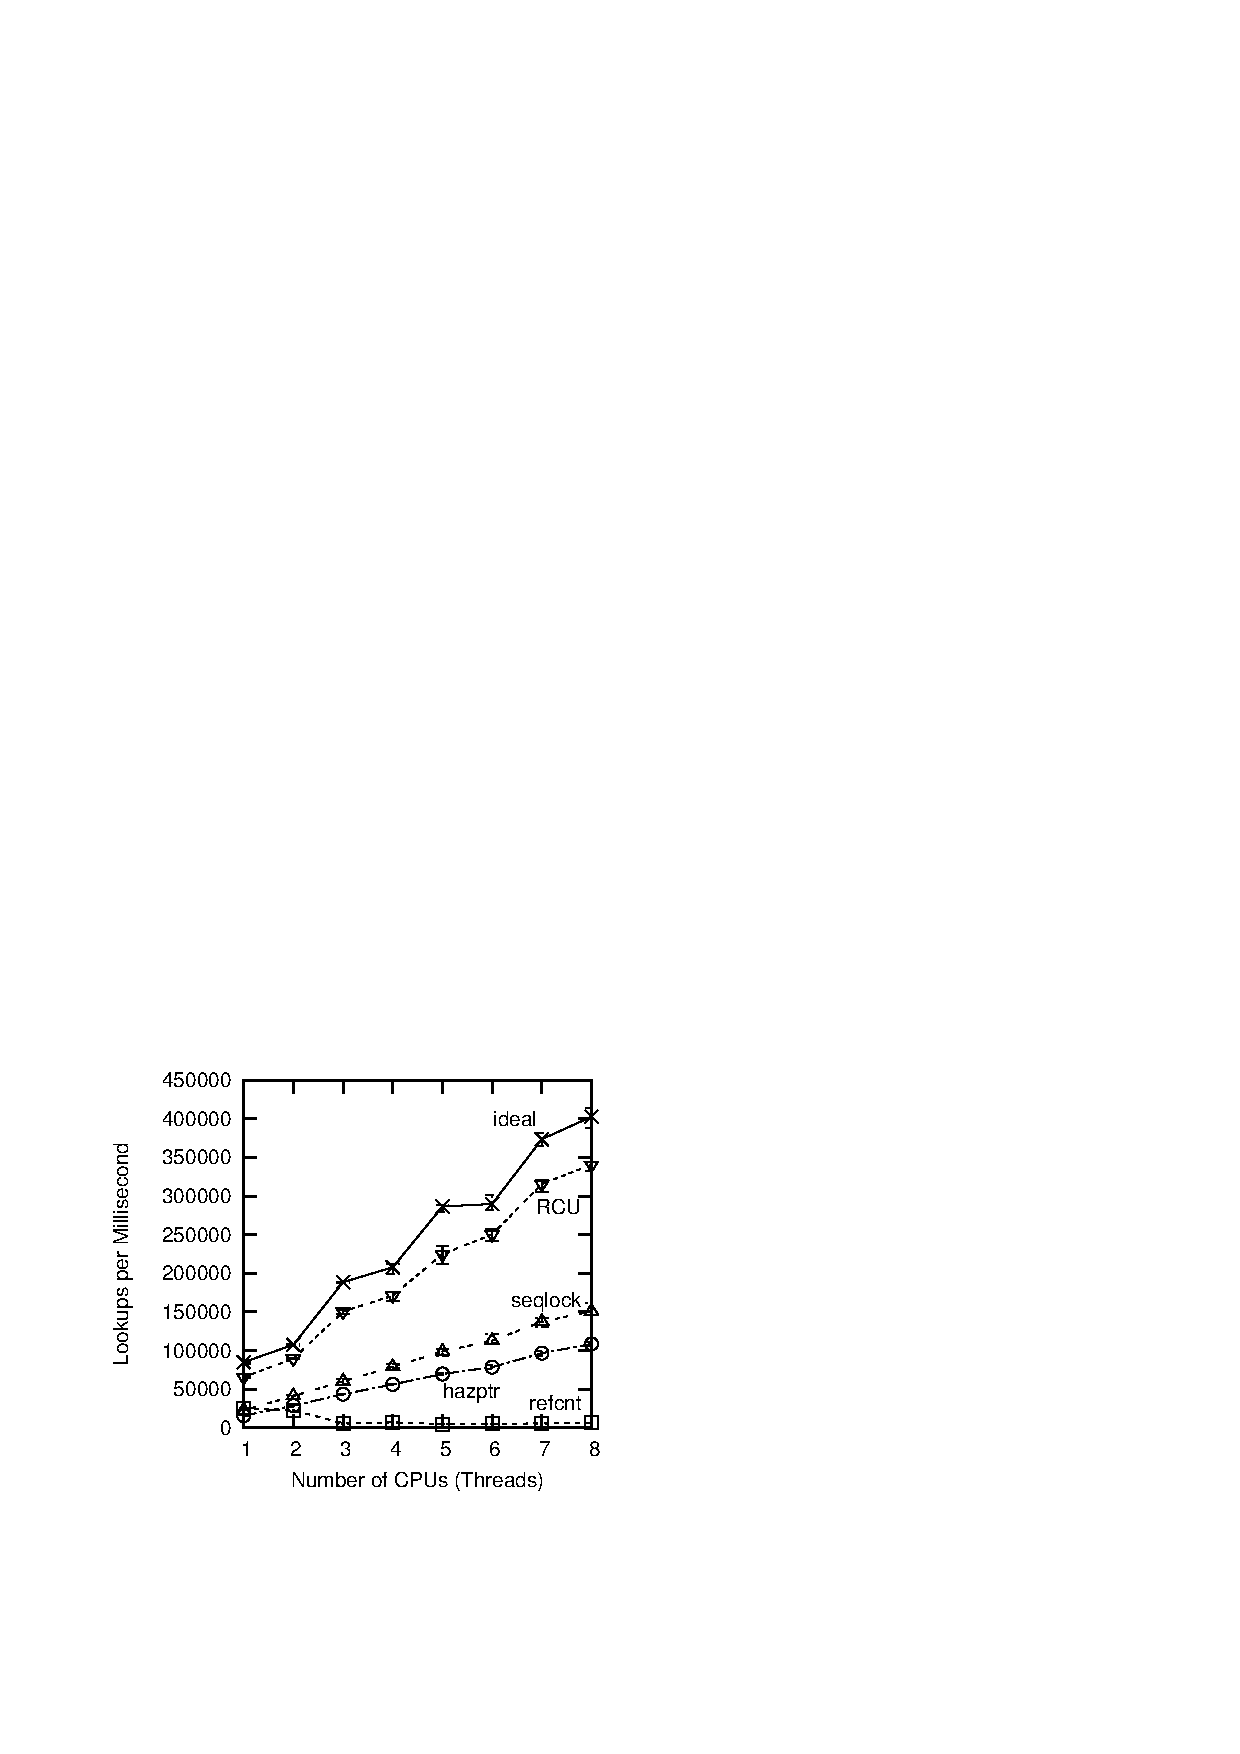
\includegraphics{CodeSamples/defer/perf-rcu}}
\caption{Pre-BSD Routing Table Protected by RCU}
\label{fig:defer:Pre-BSD Routing Table Protected by RCU}
\end{figure}

Figure~\ref{fig:defer:Pre-BSD Routing Table Protected by RCU}
는 읽기 전용 워크로드에서의 성능을 보입니다.
RCU 는 상당히 잘 확장되며 거의 이상적인 성능을 제공합니다.
하지만, 이 데이터는 \co{rcu_read_lock()} 과 \co{rcu_read_unlock()} 에 작은 양의
코드를 생성하는 userspace
RCU~\cite{MathieuDesnoyers2009URCU,PaulMcKenney2013LWNURCU} 의 \co{RCU_SIGNAL}
버전을 사용해 만들어졌습니다.
\co{rcu_read_lock()} 과 \co{rcu_read_unlock()} 에 어떤 코드도 생성하지 않는
QSBR 버전의 RCU 를 사용하면 어떻게 될까요?
(RCU QSBR 에 대한 논의를 위해선
Section~\ref{sec:defer:Introduction to RCU},
그리고 특히
Figure~\ref{fig:defer:QSBR: Waiting for Pre-Existing Readers} 를 보시기
바랍니다.)

이에 대한 답이 RCU QSBR 의 성능과 확장성은 실제로 이상적인 동기화 없는
워크로드의 것을 넘어섬을 보이는
Figure~\ref{fig:defer:Pre-BSD Routing Table Protected by RCU QSBR}
에 보여져 있습니다.

\iffalse

Figure~\ref{fig:defer:Pre-BSD Routing Table Protected by RCU}
shows the performance on the read-only workload.
RCU scales quite well, and offers nearly ideal performance.
However, this data was generated using the \co{RCU_SIGNAL}
flavor of userspace
RCU~\cite{MathieuDesnoyers2009URCU,PaulMcKenney2013LWNURCU},
for which \co{rcu_read_lock()} and \co{rcu_read_unlock()}
generate a small amount of code.
What happens for the QSBR flavor of RCU, which generates no code at all
for \co{rcu_read_lock()} and \co{rcu_read_unlock()}?
(See Section~\ref{sec:defer:Introduction to RCU},
and especially
Figure~\ref{fig:defer:QSBR: Waiting for Pre-Existing Readers},
for a discussion of RCU QSBR\@.)

The answer to this is shown in
Figure~\ref{fig:defer:Pre-BSD Routing Table Protected by RCU QSBR},
which shows that RCU QSBR's performance and scalability actually exceeds
that of the ideal synchronization-free workload.

\fi

\QuickQuizSeries{%
\QuickQuizB{
	잠깐요, 뭐라고요???
	어떻게 RCU QSBR 이 이상적인 것보다 나을 수 있죠?
	어떤 쓰레기 같은 이상에 대한 정의가 그것이 모든 가능한 결과 중 최선이
	아니게 할 수 있죠???

	\iffalse

	Wait, what???
	How can RCU QSBR possibly be better than ideal?
	Just what rubbish definition of ideal would fail to be the best
	of all possible results???

	\fi

}\QuickQuizAnswerB{
	훌륭한 질문이고, 이에 대한 답은 현대의 CPU 와 컴파일러는 굉장히
	복잡하다는 것입니다.
	하지만 거기까지 가기 전에, RCU QSBR 의 성능 이득은 코어당 하나의
	하드웨어 쓰레드가 제공되는 세계에서만 나타남을 알아둘 가치가 있습니다.
	시스템에 부하가 완전히 걸리고 나면, RCU QSBR 의 성능은 이상적인 것의
	수준으로 떨어집니다.

	RCU 버전의 \co{route_lookup()} 탐색 반복문은 실제 순차적 버전의 것보다
	x86 명령을 하나더 가지는데, 이는 \co{cmp}, \co{je}, \co{mov}, \co{cmp},
	\co{lea}, and \co{jne} 순서에서의 \co{lea} 입니다.
	이 추가된 명령은 RCU 버전의 \co{route_entry} 구조체의 시작지점에 있는
	\co{rcu_head} 구조체 때문으로, 이 때문에 순차적 버전과 달리 RCU 버전의
	\co{->re_next.next} 포인터는 0이 아닌 오프셋을 갖습니다.
	1980년대로 돌아가 보면, 이 추가적인 \co{lea} 명령은 RCU 버전이 느려지는
	결과를 낼 수도 있었습니다만, 우린 지금 21세기에 있으며, 1980년대는 한참
	지났습니다.

	\iffalse

	This is an excellent question, and the answer is that modern
	CPUs and compilers are extremely complex.
	But before getting into that, it is well worth noting that
	RCU QSBR's performance advantage appears only in the
	one-hardware-thread-per-core regime.
	Once the system is fully loaded, RCU QSBR's performance drops
	back to ideal.

	The RCU variant of the \co{route_lookup()} search loop actually
	has one more x86 instruction than does the sequential version,
	namely the \co{lea} in the sequence
	\co{cmp}, \co{je}, \co{mov}, \co{cmp}, \co{lea}, and \co{jne}.
	This extra instruction is due to the \co{rcu_head} structure
	at the beginning of the RCU variant's \co{route_entry} structure,
	so that, unlike the sequential variant, the RCU variant's
	\co{->re_next.next} pointer has a non-zero offset.
	Back in the 1980s, this additional \co{lea} instruction might
	have reliably resulted in the RCU variant being slower, but we
	are now in the 21\textsuperscript{st} century, and the 1980s
	are long gone.

	\fi

	하지만
	\cref{sec:cpu:Pipelined CPUs}
	를 주의 깊게 읽은 여러분들은 이미 이 모든 걸 알고 있을 겁니다!

	이런 반직관적인 결과는 물론 현대 마이크로프로세서에서의 모든 성능
	결과는 약간 회의적으로 보아져야 함을 의미합니다.
	이론상, 이상적인 것보다 나은 성능을 얻는다는 것은 정말 말이 안됩니다만,
	현대의 마이크로프로세서에서는 정말로 일어날 수 있는 일입니다.
	그런 결과는 축복받은 초선형적 성능향상 (그런 예 중 하나를 위해
	Section~\ref{sec:SMPdesign:Beyond Partitioning} 을 보세요) 비슷한 걸로
	생각 될 수 있는데, 즉, 흥미롭지만 또한 실용적 중요도는 제한된다는
	것입니다.
	그러나, RCU 의 강점 중 하나는 그 읽기 쪽 오버헤드가 무척 낮아서 이와
	같은 작은 효과가 실제 성능 측정에도 보여질 수 있다는 것입니다.

	\iffalse

	But those of you who read
	\cref{sec:cpu:Pipelined CPUs}
	carefully already knew all of this!

	These counter-intuitive results of course means that any
	performance result on modern microprocessors must be subject to
	some skepticism.
	In theory, it really does not make sense to obtain performance
	results that are better than ideal, but it really can happen
	on modern microprocessors.
	Such results can be thought of as similar to the celebrated
	super-linear speedups (see
	Section~\ref{sec:SMPdesign:Beyond Partitioning}
	for one such example), that is, of interest but also of limited
	practical importance.
	Nevertheless, one of the strengths of RCU is that its read-side
	overhead is so low that tiny effects such as this one are visible
	in real performance measurements.

	\fi

\begin{figure}[tb]
\centering
\resizebox{2.5in}{!}{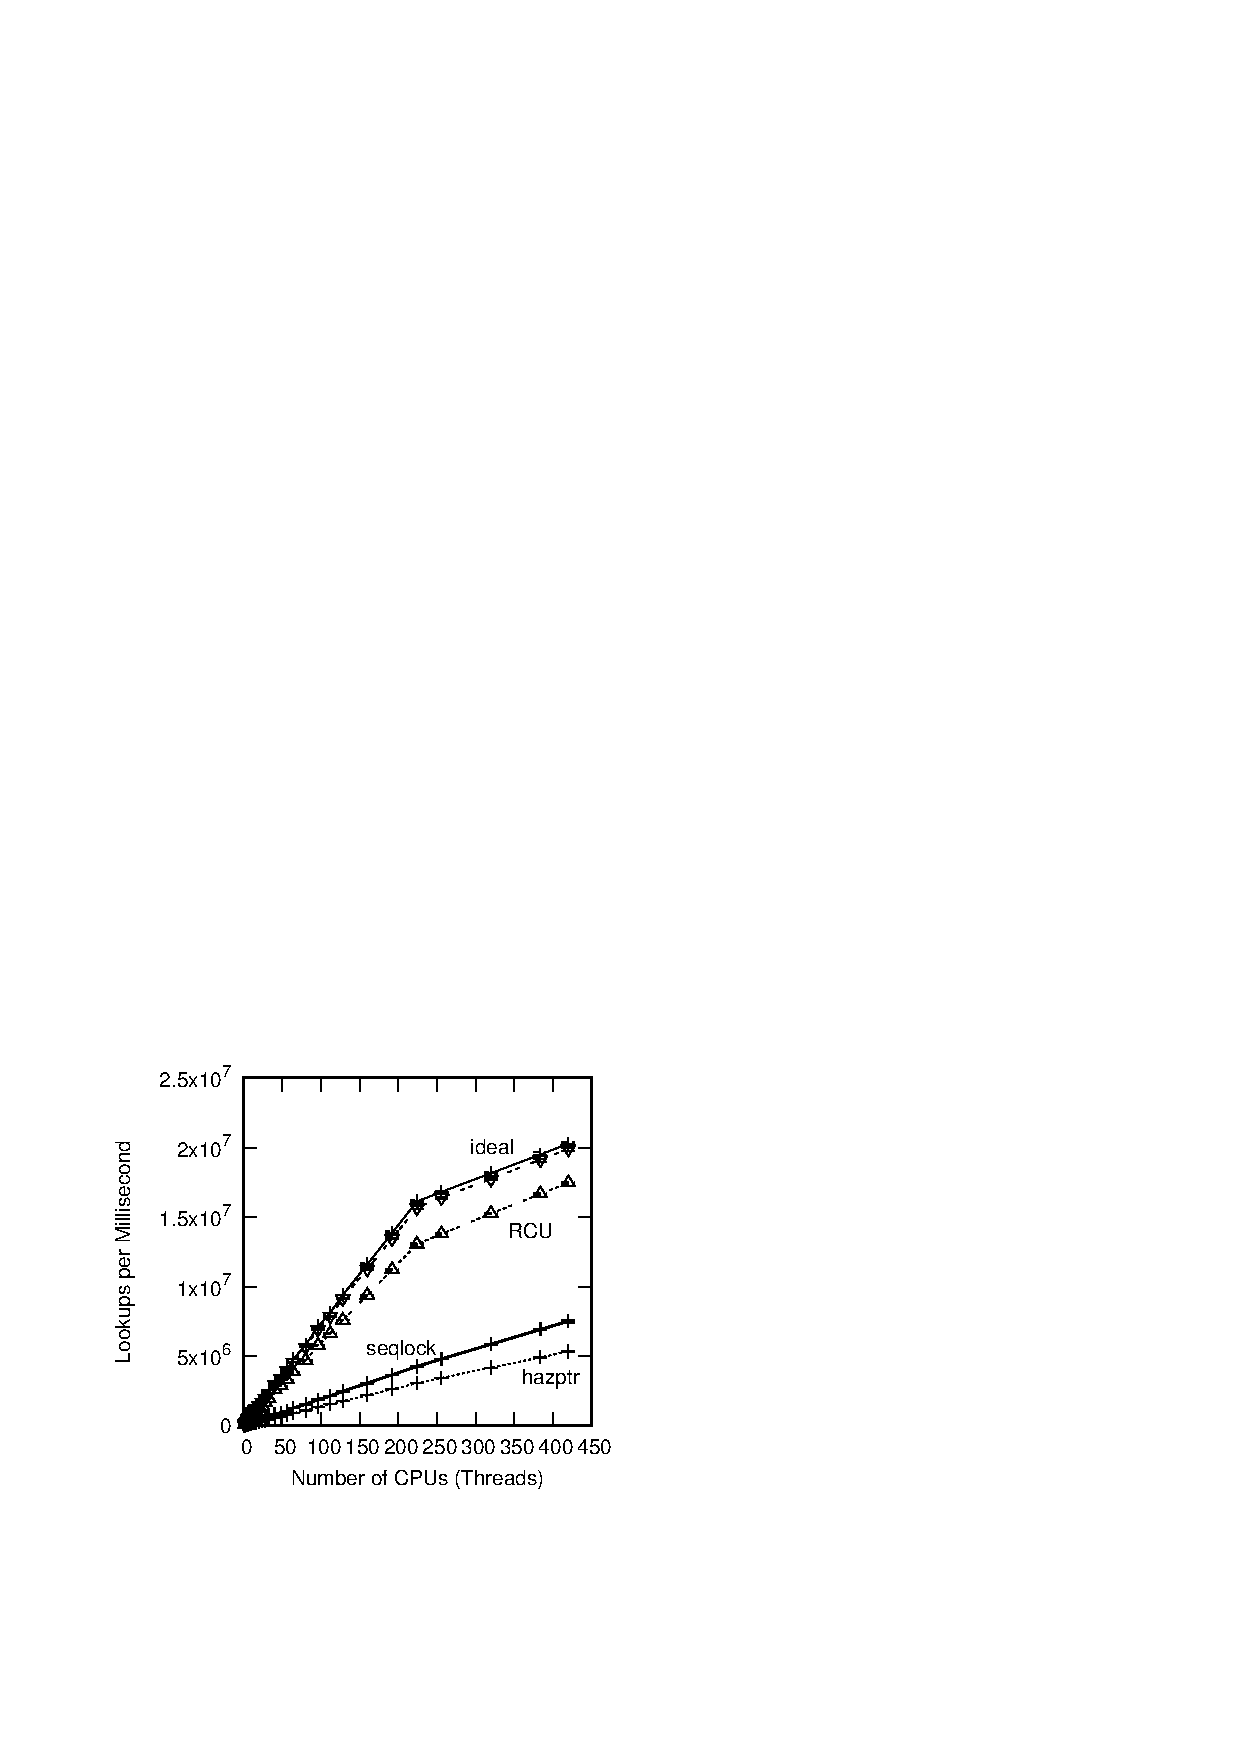
\includegraphics{CodeSamples/defer/perf-rcu-qsbr-qq}}
\caption{Pre-BSD Routing Table Protected by RCU QSBR With Non-Initial \tco{rcu_head}}
\label{fig:defer:Pre-BSD Routing Table Protected by RCU QSBR With Non-Initial rcu-head}
\end{figure}

	이는 \co{rcu_head} 구조체가 \co{->re_next.next} 포인터가 0 오프셋을
	갖게끔 옮겨져서 순차적 버전과 동일하게 되면 어떻게 되는지 질문을 하게
	만듭니다.
	그에 대한 답은
	Figure~\ref{fig:defer:Pre-BSD Routing Table Protected by RCU QSBR With Non-Initial rcu-head}
	에 보여져 있듯, RCU QSBR 의 성능이 여전히 이상적인 것에 근접하지만
	이상적인 것을 넘어서지는 않게 한다는 것입니다.

	\iffalse

	This raises the question as to what would happen if the
	\co{rcu_head} structure were to be moved so that RCU's
	\co{->re_next.next} pointer also had zero offset, just the
	same as the sequential variant.
	And the answer, as can be seen in
	Figure~\ref{fig:defer:Pre-BSD Routing Table Protected by RCU QSBR With Non-Initial rcu-head},
	is that this causes RCU QSBR's performance to decrease to where
	it is still very nearly ideal, but no longer super-ideal.

	\fi

}\QuickQuizEndB
%
\QuickQuizE{
	RCU QSBR 의 읽기 성능이 그렇게 좋은데, 왜 다른 userspace 버전을
	신경쓰죠?

	\iffalse

	Given RCU QSBR's read-side performance, why bother with any
	other flavor of userspace RCU?

	\fi

}\QuickQuizAnswerE{
	RCU QSBR 은 허용될 수 없을 수도 있는 어플리케이션 전체의 제약을
	요구하기 때문인데, 예를 들면 어플리케이션 내의 모든 각각의 쓰레드가
	정기적으로 quiescent state 를 지나야 한다는 것입니다.
	다른 것들 중에서도, 이는 RCU QSBR 이 다른 종류의 userspace
	RCU~\cite{PaulMcKenney2013LWNURCU} 에 의해 더 잘 도움받을 수도 있는
	라이브러리 작성자에게는 도움이 될 수 있다는 것을 의미합니다.

	\iffalse

	Because RCU QSBR places constraints on the overall application
	that might not be tolerable,
	for example, requiring that each and every thread in the
	application regularly pass through a quiescent state.
	Among other things, this means that RCU QSBR is not helpful
	to library writers, who might be better served by other
	flavors of userspace RCU~\cite{PaulMcKenney2013LWNURCU}.

	\fi

}\QuickQuizEndE
}

\begin{figure}[tb]
\centering
\resizebox{2.5in}{!}{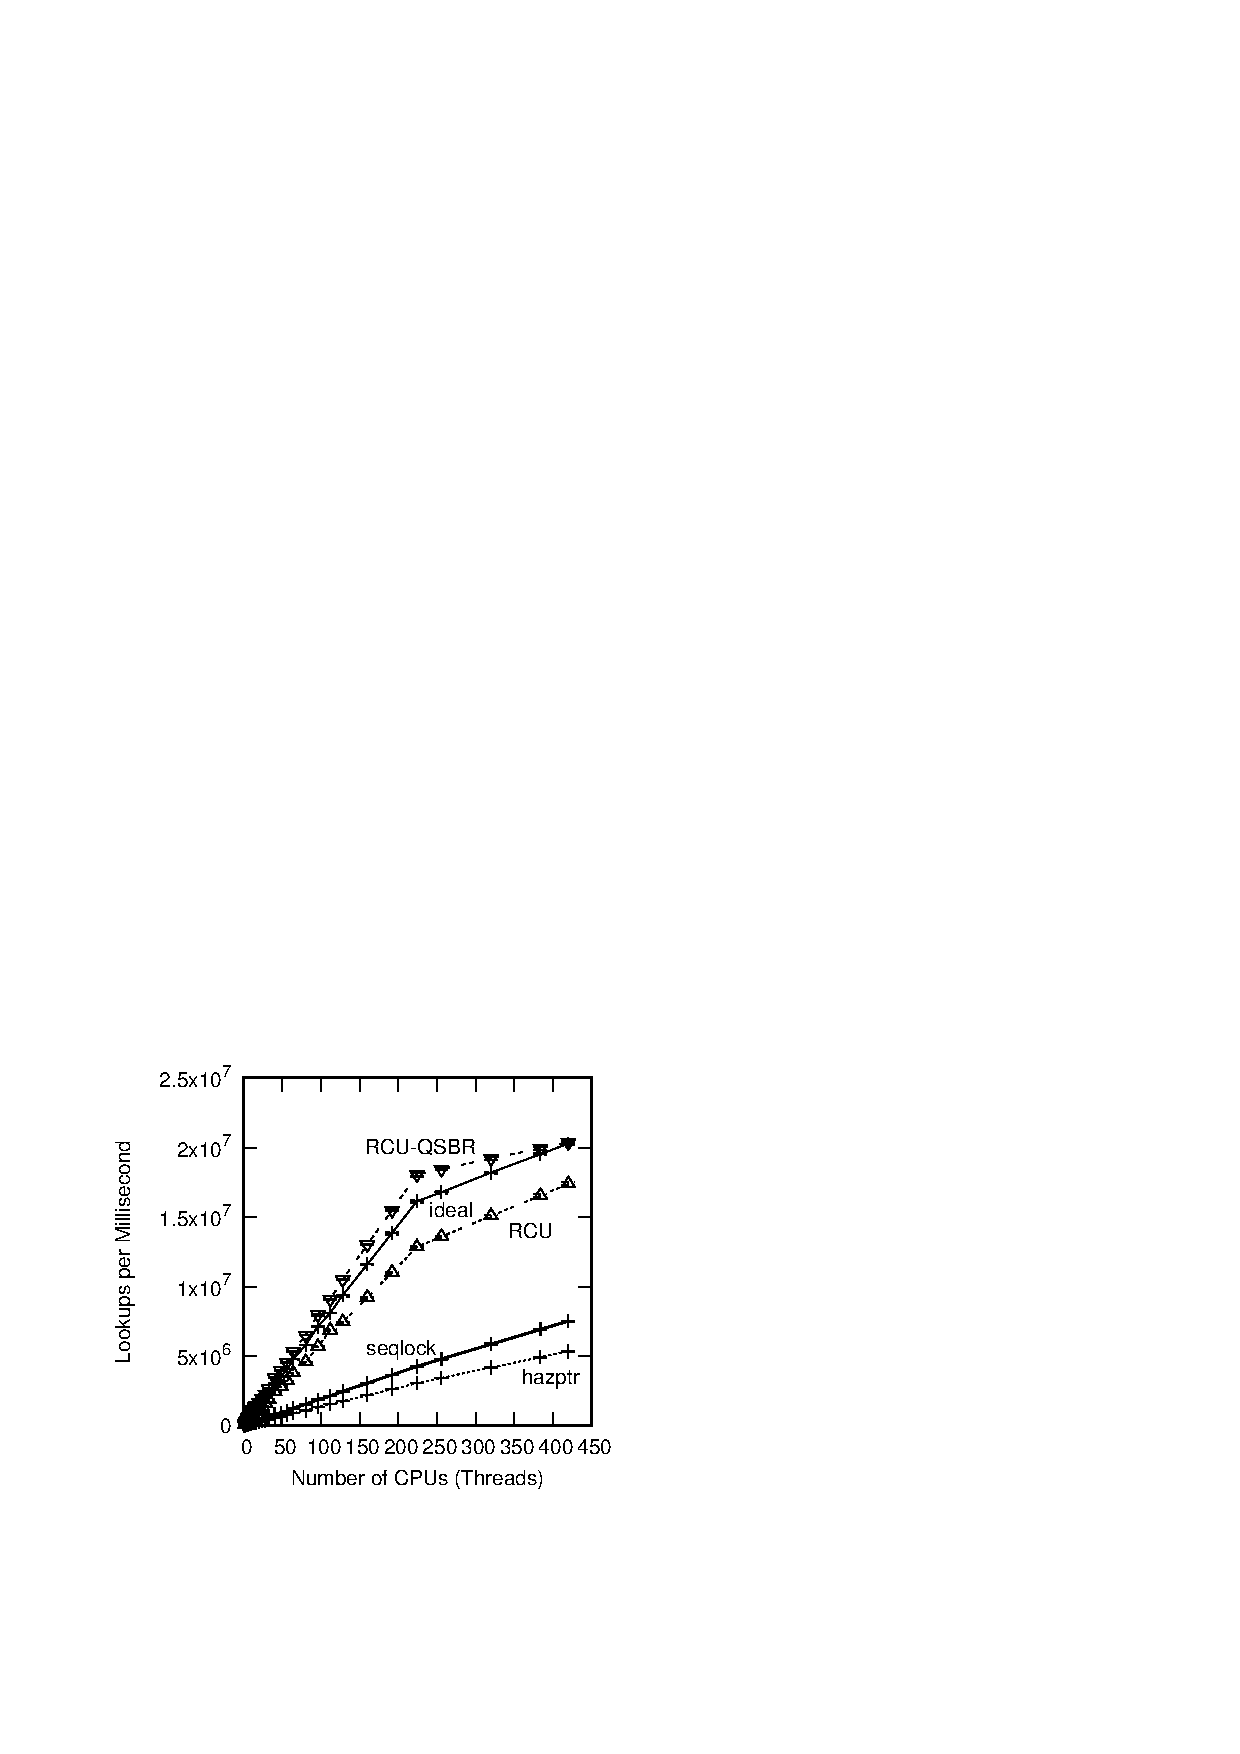
\includegraphics{CodeSamples/defer/perf-rcu-qsbr}}
\caption{Pre-BSD Routing Table Protected by RCU QSBR}
\label{fig:defer:Pre-BSD Routing Table Protected by RCU QSBR}
\end{figure}

\subsubsection{RCU is a Reader-Writer Lock Replacement}
\label{sec:defer:RCU is a Reader-Writer Lock Replacement}

리눅스 커널에서의 RCU 의 가장 흔한 사용처는 아마도 읽기가 집중적인 상황에서의
reader-writer 락킹 대체일 겁니다.
그러나, 이런 RCU 사용은 처음에 제게 즉각적으로 적절하게 느껴지지 않았고, 실제로
저는 1990년대 초에 범용 RCU 구현을 만들기 전에 가벼운 reader-writer 락을
구현하기로 했습니다~\cite{WilsonCHsieh92a}.\footnote{
	2.4 리눅스 커널의 \co{brlock} 과, 더 최신의 리눅스 커널의 \co{lglock}
	과 비슷합니다.}
이 가벼운 reader-writer 락으로 제가 하고자 했던 모든 것은 결국 RCU 를 이용해
구현되었습니다.
사실, 그건 이 가벼운 reader-writer 락이 처음 사용되기 3년이나 전의
일이었습니다.
정말 바보가 된 것 같았죠!

RCU 와 reader-writer 락킹 사이의 핵심 유사성은 둘 다 병렬로 구생될 수 있는
read-side 크리티컬 섹션을 갖는다는 것입니다.
실제로, 어떤 경우에는 RCU API 멤버들을 연관된 reader-writer 락 API 멤버들로
대체하는게 가능합니다.
하지만 무엇보다, 왜 그런걸 신경쓰죠?

\iffalse

Perhaps the most common use of RCU within the Linux kernel is as
a replacement for reader-writer locking in read-intensive situations.
Nevertheless, this use of RCU was not immediately apparent to me
at the outset, in fact, I chose to implement a lightweight reader-writer
lock~\cite{WilsonCHsieh92a}\footnote{
	Similar to \co{brlock} in the 2.4 Linux kernel and to
	\co{lglock} in more recent Linux kernels.}
before implementing a general-purpose RCU implementation
back in the early 1990s.
Each and every one of the uses I envisioned for the lightweight reader-writer
lock was instead implemented using RCU\@.
In fact, it was more than
three years before the lightweight reader-writer lock saw its first use.
Boy, did I feel foolish!

The key similarity between RCU and reader-writer locking is that
both have read-side critical sections that can execute in parallel.
In fact, in some cases, it is possible to mechanically substitute RCU API
members for the corresponding reader-writer lock API members.
But first, why bother?

\fi

RCU 의 장점은 성능, 데드락 내성, 그리고 리얼타임 응답시간을 포함합니다.
물론, RCU 의 제한점들도 존재하는데 읽기 쓰레드와 업데이트 쓰레드가 동시에
수행된다는 사실, 낮은 우선순위 RCU 읽기 쓰레드가 높은 우선순위 쓰레드를 grace
period 하나가 지나갈 때까지 블록시킨다는 것, 그리고 grace period 응답시간이 수
밀리세컨드까지 길어질 수 있다는 점이 포함됩니다.
이런 장점과 한계점들이 다음 문단들에서 논의됩니다.

\iffalse

Advantages of RCU include performance,
deadlock immunity, and realtime latency.
There are, of course, limitations to RCU, including the fact that
readers and updaters run concurrently, that low-priority RCU readers
can block high-priority threads waiting for a grace period to elapse,
and that grace-period latencies can extend for many milliseconds.
These advantages and limitations are discussed in the following paragraphs.

\fi

\paragraph{Performance}

\begin{figure}[tb]
\centering
\resizebox{2.5in}{!}{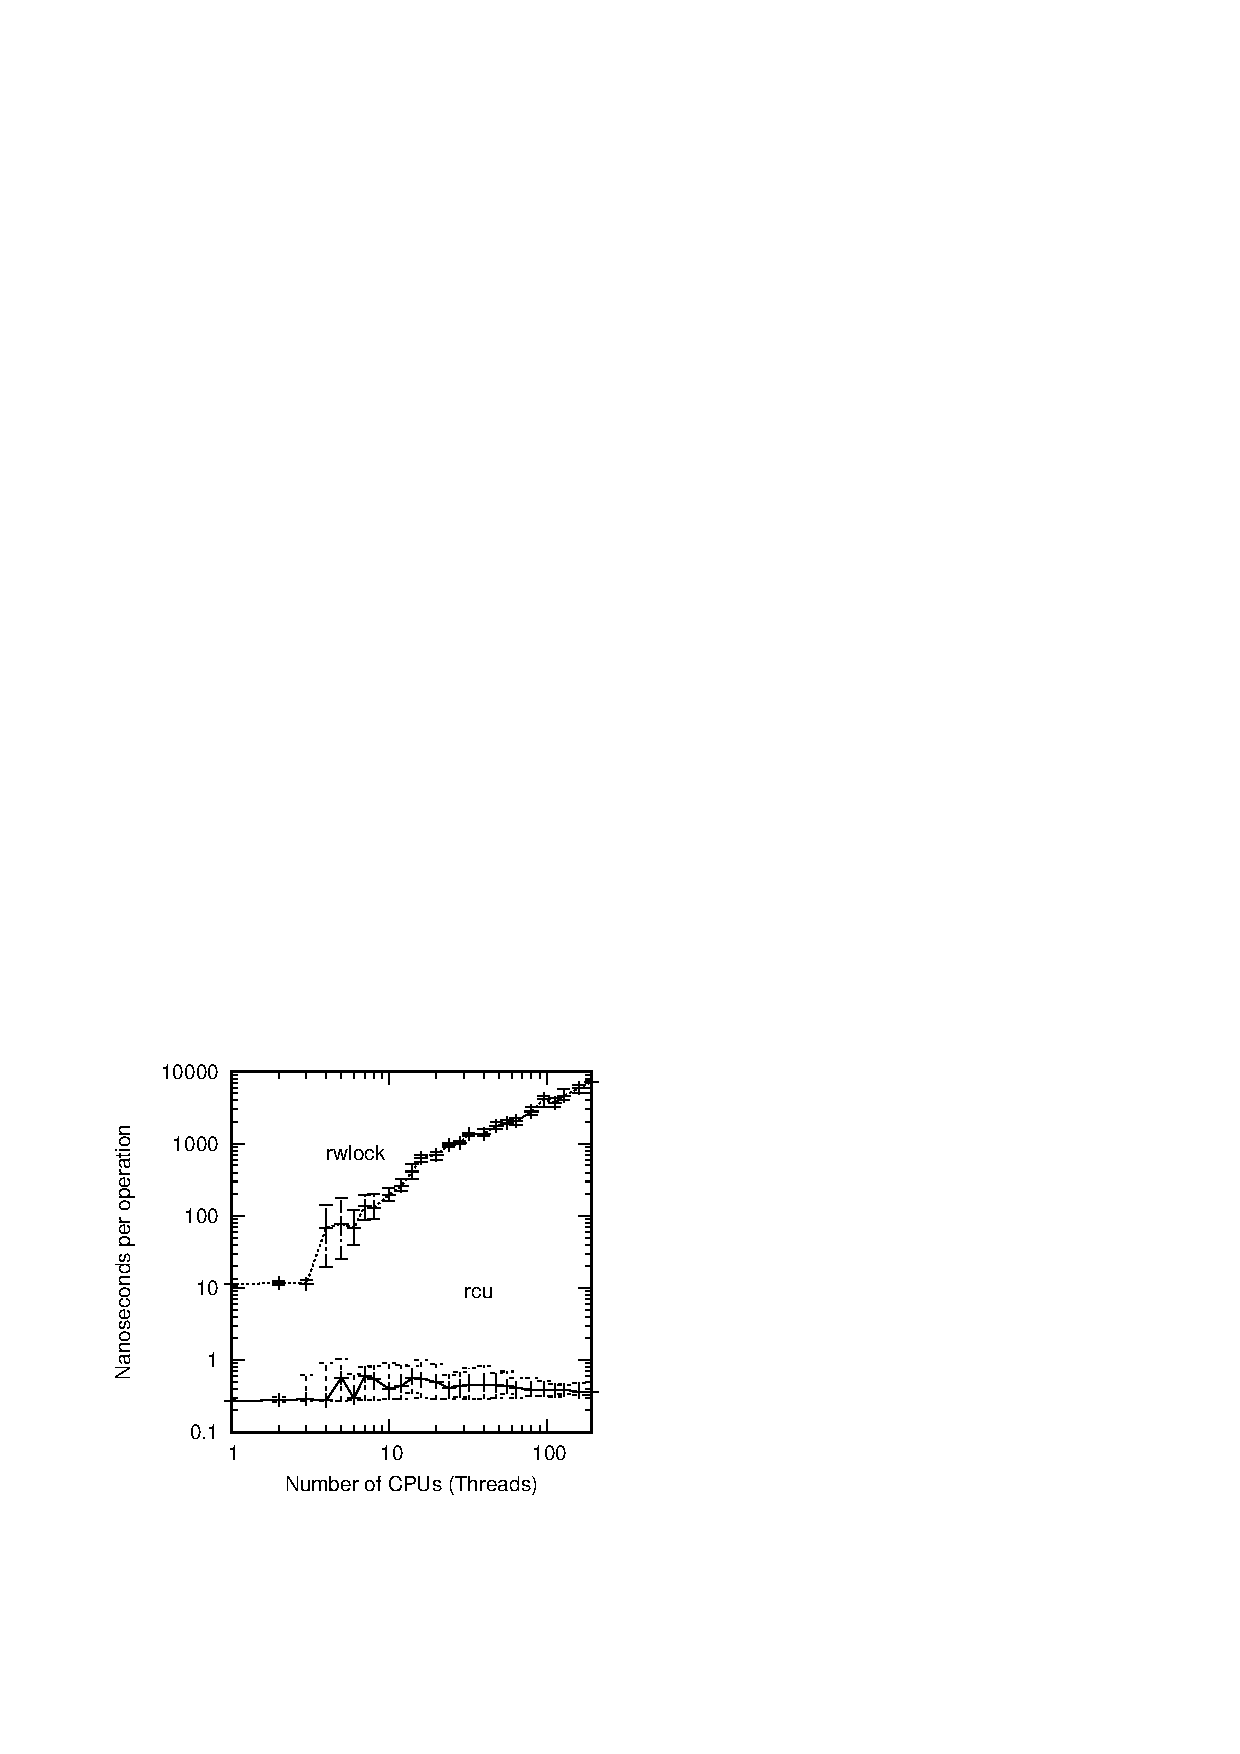
\includegraphics{defer/rwlockRCUperf}}
\caption{Performance Advantage of RCU Over Reader-Writer Locking}
\label{fig:defer:Performance Advantage of RCU Over Reader-Writer Locking}
\end{figure}

리눅스 커널 RCU 의 reader-writer 락킹 대비 읽기 성능 장점이
448 개 2.10\,GHz Intel x86 CPU 시스템에서 측정되어 만들어진
Figure~\ref{fig:defer:Performance Advantage of RCU Over Reader-Writer Locking}
에 보여져 있습니다.

\iffalse

The read-side performance advantages of Linux-kernel RCU over
reader-writer locking are shown in
Figure~\ref{fig:defer:Performance Advantage of RCU Over Reader-Writer Locking},
which was generated on a 448-CPU 2.10\,GHz Intel x86 system.

\fi

\QuickQuizSeries{%
\QuickQuizB{
	뭐요?
	2.10\,GHz 에서의 클락 시간은 약 500\,picosecond 인데 RCU 가
	300-picosecond 도 안되는 오버헤드를 갖는다는 말을 나더러 믿으라구요?

	\iffalse

	WTF?
	How the heck do you expect me to believe that RCU can have less
	than a 300-picosecond overhead when the clock period at 2.10\,GHz
	is almost 500\,picoseconds?

	\fi

}\QuickQuizAnswerB{
	우선, 이 측정을 위해 사용된 반복문이 다음과 같음을 고려합시다:

	\iffalse

	First, consider that the inner loop used to
	take this measurement is as follows:

	\fi

\begin{VerbatimN}
	for (i = nloops; i >= 0; i--) {
		rcu_read_lock();
		rcu_read_unlock();
	}
\end{VerbatimN}

	다음으로, 실질적인 \co{rcu_read_lock()} 과 \co{rcu_read_unlock()} 의
	정의를 생각해 봅시다:

	\iffalse

	Next, consider the effective definitions of \co{rcu_read_lock()}
	and \co{rcu_read_unlock()}:

	\fi

\begin{VerbatimN}
#define rcu_read_lock()   barrier()
#define rcu_read_unlock() barrier()
\end{VerbatimN}

	이 정의들은 메모리 참조에 연관되는 컴파일러의 코드 이동 최적화를
	제약하지만, 그것들 자체 내에는 어떤 명령도 넣지 않습니다.
	하지만, 이 반복문 변수가 레지스터에 관리된다면, \co{i} 로의 액세스는
	메모리 참조로 취급되지 않습니다.
	더욱이, 컴파일러는 loop unrolling 을 알 수 있어, 결과적인 코드가 단순히
	\co{i} 값을 1보다 큰 어떤 값으로 증가시키는 것으로 여러 횟수의 반복문
	수행을 ``해내는'' 코드를 만들 수 있습니다.

	따라서 267 picoseconds 의 ``측정'' 은 시간 측정을 \co{rcu_read_lock()}
	과 \co{rcu_read_unlock()} 호출을 포함하는 이 내부 반복문을 통과하는
	반복 횟수로 나눈 것에 이 loop-unrolling 으로 \co{i} 조정 코드를 나눈
	것을 더한 고정된 오버헤드입니다.
	그리고 그래서, 이 측정은 실제로 에러를 포함하고 있으며, 실제로
	오버헤드를 수십 수백배로 부풀려서 이야기 하고 있습니다.
	어쨌건, 만들어진 기계 명령어의 관점에서, \co{rcu_read_lock()} 과
	\co{rcu_read_unlock()} 의 오버헤드는 정확히 제로입니다.

	267 picosecond 의 측정된 시간이 과장된 수치임이 드러나는 건 매일 있는
	일은 분명 아닙니다!

	\iffalse

	These definitions constrain compiler code-movement optimizations
	involving memory references, but emit no instructions in and
	of themselves.
	However, if the loop variable is maintained in a register,
	the accesses to \co{i} will not count as memory references.
	Furthermore, the compiler can do loop unrolling,
	allowing the resulting code to ``execute'' multiple passes
	through the loop body simply by incrementing \co{i} by
	some value larger than the value 1.

	So the ``measurement'' of 267 picoseconds is simply the fixed
	overhead of the timing measurements divided by the number of
	passes through the inner loop containing the calls
	to \co{rcu_read_lock()} and \co{rcu_read_unlock()}, plus
	the code to manipulate \co{i} divided by the loop-unrolling
	factor.
	And therefore, this measurement really is in error, in fact,
	it exaggerates the overhead by an arbitrary number of orders
	of magnitude.
	After all, in terms of machine instructions emitted, the actual
	overheads of \co{rcu_read_lock()} and of \co{rcu_read_unlock()}
	are each precisely zero.

	It certainly is not just every day that a timing measurement
	of 267 picoseconds turns out to be an overestimate!

	\fi
}\QuickQuizEndB

\QuickQuizM{
	이 책의 초기 버전에서는 RCU 읽기 오버헤드가 1 picosecond 미만이라 하지
	않았나요?
	무슨 일이 있었던 거죠???

	\iffalse

	Didn't an earlier release of this book show RCU read-side
	overhead way down in the sub-picosecond range?
	What happened???

	\fi

}\QuickQuizAnswerM{
	훌륭한 기억력이군요!!!
	어떤 초기 버전에서의 오버헤드는 실제로 약 100 femtosecond 이었습니다.

	그사이 무슨 일이 있었느냐면, RCU 사용처가 리눅스 커널 내에 더욱 널리
	퍼졌는데, page fault 처리 코드도 여기 포함됩니다.
	그때로 돌아가면, \co{rcu_read_lock()} 과 \co{rcu_read_unlock()} 은
	\co{CONFIG_PREEMPT=n} 커널에서 완전히 아무 일도 하지 않았습니다.
	불행히도, 그 상황은 컴파일러가 page fault 되는 메모리 액세스를 RCU
	read-side 크리티컬 섹션 내로 재배치 할 수 있게 했습니다.
	물론, page fault 는 블록될 수 있으며, 따라서 이 크리티컬 섹션을
	망가지게 합니다.

	\iffalse

	Excellent memory!!!
	The overhead in some early releases was in fact roughly
	100~femtoseconds.

	What happened was that RCU usage spread more broadly through the
	Linux kernel, including into code that takes page faults.
	Back at that time, \co{rcu_read_lock()} and \co{rcu_read_unlock()}
	were complete no-ops in \co{CONFIG_PREEMPT=n} kernels.
	Unfortunately, that situation allowed the compiler to reorder
	page-faulting memory accesses into RCU read-side critical
	sections.
	Of course, page faults can block, which destroys those critical
	section.

	\fi

	이건 이론적 문제만이 아니었습니다:
	그로 인한 문제가 실제로 2019년에 이야기 되었습니다.
	\ppl{Herber}{Xu} 는 이 문제를 분석했고 \ppl{Linus}{Torvalds} 는
	\co{rcu_read_lock()} 과 \co{rcu_read_unlock()} 이 무조건적으로
	\co{barrier()} 호출을 포함하게 하는 커밋을 대기열에
	올렸습니다~\cite{LinusTorvalds2019:RCUreader.barrier}.
	그리고 \co{barrier()} 가 코드를 추가하진 않지만, 컴파일러 최적화를
	제한합니다.
	따라서 널리 퍼져있는 RCU 사용처의 비용은 \co{rcu_read_lock()} 과
	\co{rcu_read_unlock()} 오버헤드보다 약간 더 높아집니다.

	물론, 더 오래전의 결과는
	Figure~\ref{fig:defer:Performance Advantage of RCU Over Reader-Writer Locking}
	에서 보인 것과 다른 시스템에서 얻어진 겁니다.
	그래서 뭐가 더 영향을 끼쳤을까요, Linus 의 커밋 또는 시스템 변경?
	이 질문은 독자 여러분의 연습문제로 남겨둡니다.

	\iffalse

	Nor was this a theoretical problem:
	A failure actually manifested in 2019.
	\ppl{Herbert}{Xu} tracked down this failure down and
	\ppl{Linus}{Torvalds}
	therefore queued a commit to upgrade \co{rcu_read_lock()} and
	\co{rcu_read_unlock()} to unconditionally include a call to
	\co{barrier()}~\cite{LinusTorvalds2019:RCUreader.barrier}.
	And although \co{barrier()} emits no code, it does constrain
	compiler optimizations.
	And so the price of widespread RCU usage is slightly higher
	\co{rcu_read_lock()} and \co{rcu_read_unlock()} overhead.

	Of course, it is also the case that the older results were obtained
	on a different system than were those shown in
	Figure~\ref{fig:defer:Performance Advantage of RCU Over Reader-Writer Locking}.
	So which change had the most effect, Linus's commit or the change in
	the system?
	This question is left as an exercise to the reader.

	\fi

}\QuickQuizEndM

\QuickQuizE{
	Figure~\ref{fig:defer:Performance Advantage of RCU Over Reader-Writer Locking}
	의 \co{rcu} 에는 왜그리 큰 편차가 존재하는 거죠?

	\iffalse

	Why is there such large variation for the \co{rcu} trace in
	Figure~\ref{fig:defer:Performance Advantage of RCU Over Reader-Writer Locking}?

	\fi

}\QuickQuizAnswerE{
	이는 log-log 그림이며, 따라서 크게 보이는 \co{rcu} 편차는 실제로는 수백
	picosecond 에 불과함을 명심하세요.
	그리고 그건 무엇이든 그것을 일으킬 수 있는 무척 짧은 시간입니다.
	하지만, 편차가 CPU 수가 작든 크든 감소된다는 걸로 보아, 한가지 가능한
	가설은 이 편차는 하나의 CPU 에서 다른 CPU 로의 migration 때문이라는
	것입니다.

	그래요, 이 측정은 인터럽트가 불능화 된 채로 취해졌습니다만, 게스트 OS
	내에서 취해졌으므로, 하이퍼바이저 단계에서의 preemption 은 가능합니다.
	이 게스트 OS 들을 리얼타임 우선순위로 수행함으로써 이런 편차를 줄이려는
	노력은 (Joel Fernandes 에 의해 제안되었습니다) 독자 여러분의 연습문제로
	남겨두겠습니다.

	\iffalse

	Keep in mind that this is a log-log plot, so those large-seeming
	\co{rcu} variances in reality span only a few hundred picoseconds.
	And that is such a short time that anything could cause it.
	However, given that the variance decreases with both small and
	large numbers of CPUs, one hypothesis is that the variation is
	due to migrations from one CPU to another.

	Yes, these measurements were taken with interrupts disabled, but
	they were also taken within a guest OS, so that preemption was
	still possible at the hypervisor level.
	Attempting to reduce these variations by running the guest OSes
	at real-time priority (as suggested by Joel Fernandes) is left
	as an exercise for the reader.

	\fi

}\QuickQuizEndE
}                 % End of \QuickQuizSeries

Reader-writer 락킹은 단일 CPU 에서 RCU 보다 수십배 느리며, 192~CPU 에서는
\emph{수만} 배보다 더 느리다는 것을 보시기 바랍니다.
대조적으로, RCU 는 상당히 잘 확장합니다.
두 경우 모드, 에러 바들은 30회의 측정 결과 전체 범위를 보이며, 선은 그 중간값을
보입니다.

\iffalse

Note that reader-writer locking is more than an order of magnitude slower
than RCU on a single CPU, and is more than \emph{four} orders of magnitude
slower on 192~CPUs.
In contrast, RCU scales quite well.
In both cases, the error bars cover the full range of the measurements
from 30~runs, with the line being the median.

\fi

\begin{figure}[tb]
\centering
\resizebox{2.5in}{!}{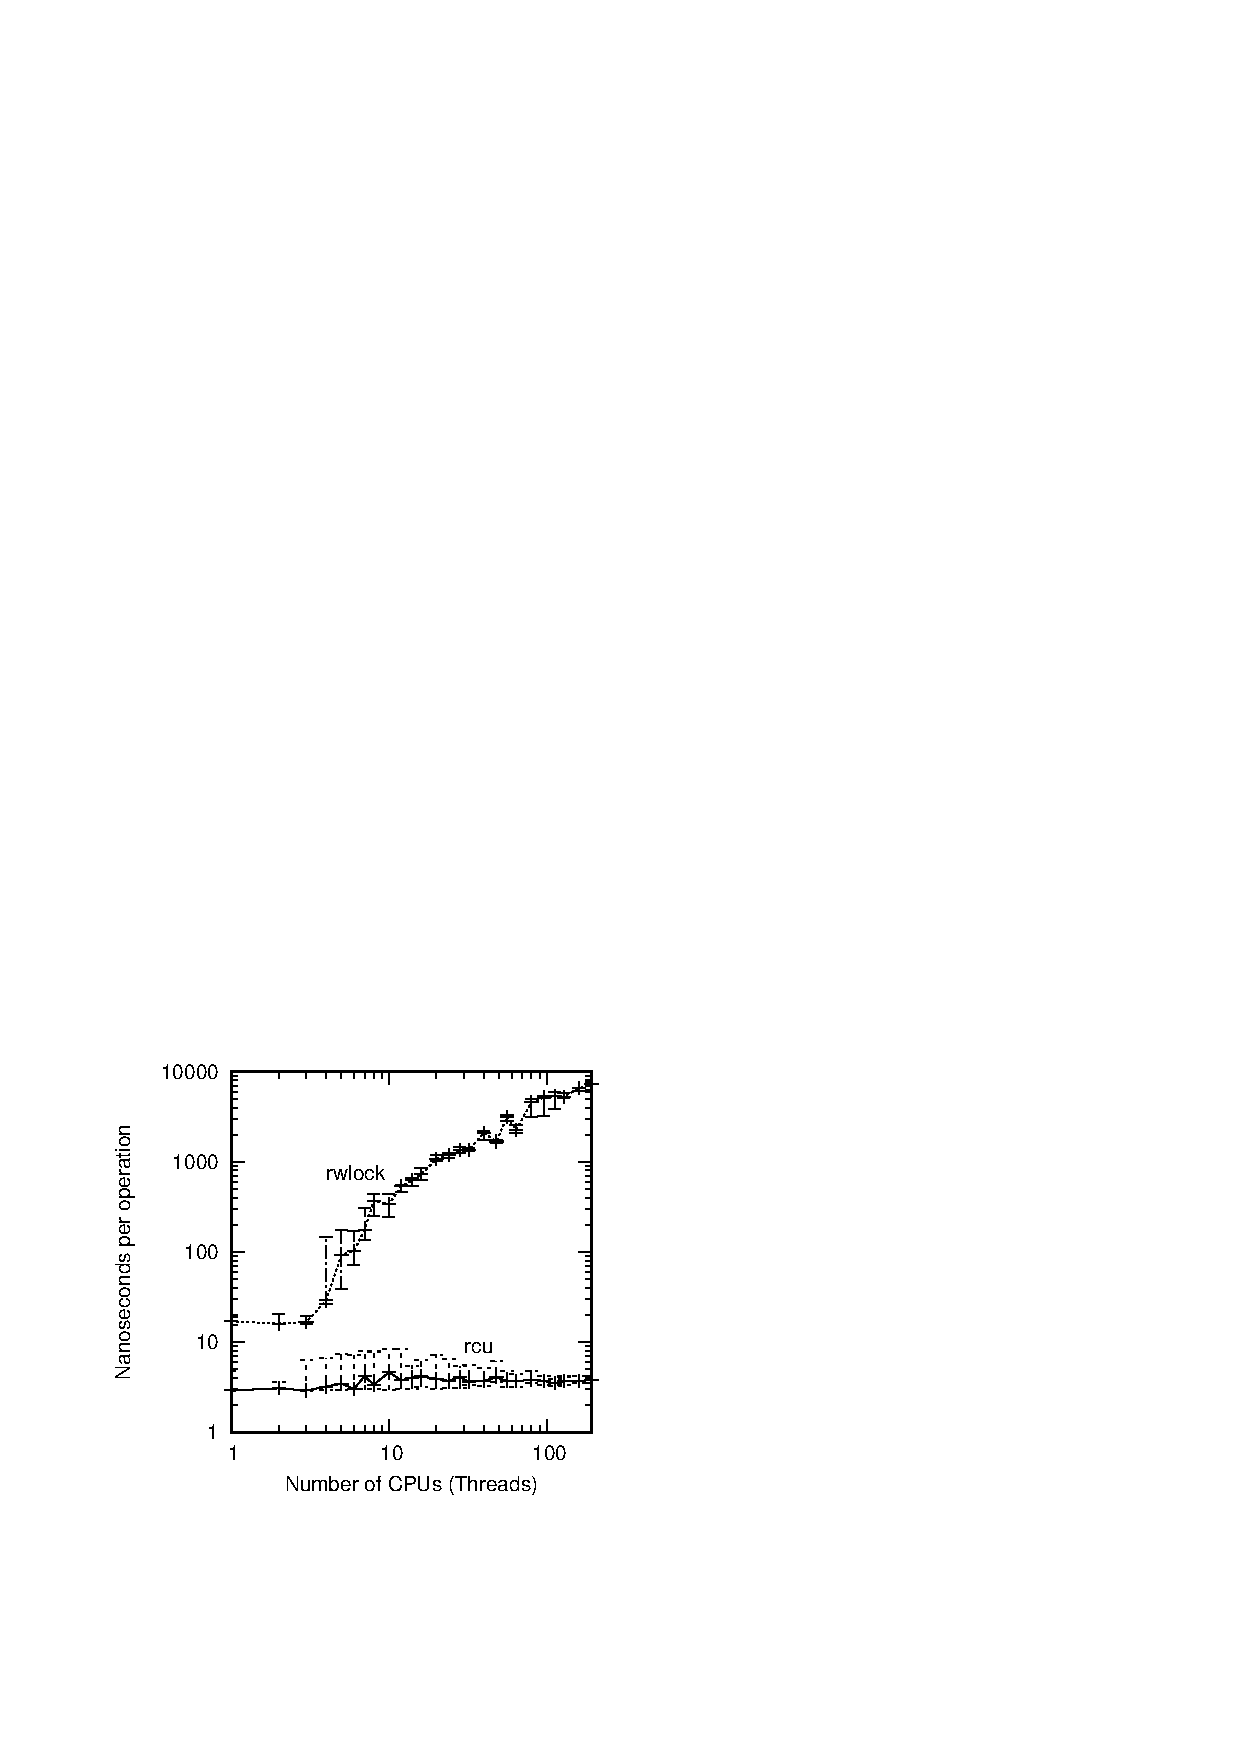
\includegraphics{defer/rwlockRCUperfPREEMPT}}
\caption{Performance Advantage of Preemptible RCU Over Reader-Writer Locking}
\label{fig:defer:Performance Advantage of Preemptible RCU Over Reader-Writer Locking}
\end{figure}

더 정확한 그림은 \co{CONFIG_PREEMPT} 커널에서 얻어질 수 있겠지만, 448rodml
2.10\,GHz x86 CPU 시스템에서 측정된
Figure~\ref{fig:defer:Performance Advantage of Preemptible RCU Over Reader-Writer Locking}
에 보이듯 RCU 는 여전히 단일 CPU 에서 약 일곱배, 192~CPU 에서 수천배
reader-writer 락보다 빠릅니다.
큰 수의 CPU 에서 reader-writer 락킹의 높은 편차값을 보세요.
에러바는 데이터의 전체 범위를 그립니다.

\iffalse

A more moderate view may be obtained from a \co{CONFIG_PREEMPT} kernel,
though RCU still beats reader-writer locking by between a factor of seven
on a single CPU and by three orders of magnitude on 192~CPUs, as shown in
Figure~\ref{fig:defer:Performance Advantage of Preemptible RCU Over Reader-Writer Locking},
which was generated on the same 448-CPU 2.10\,GHz x86 system.
Note the high variability of reader-writer locking at larger numbers of CPUs.
The error bars span the full range of data.

\fi

\QuickQuiz{
	시스템은 448 개의 하드웨어 쓰레드를 갖는데, 왜 192~CPU 까지만
	측정하나요?

	\iffalse

	Given that the system had no fewer than 448~hardware threads,
	why only 192~CPUs?

	\fi

}\QuickQuizAnswer{
	이 데이터를 생성하는데 사용된 스크립트 (\path{rcusclae.sh}) 는 모아지는
	지점들의 각 집합을 위해 게스트 운영체제를 시작하며, 이 특정
	시스템에서는 \co{qemu} 와 KVM 이 모두 특정 게스트 OS 에 설정될 수 있는
	CPU 갯수에 제한을 두기 때문입니다.
	그래요, 조금 더 많은 CPU 를 사용하는 것도 가능하겠습니다만 256 은
	불가능하다는 점을 생각할 때 이진수 관점에서 192 는 괜찮은 어림수입니다.

	\iffalse

	Because the script (\path{rcuscale.sh}) that generates this data
	spawn a guest operating system for each set of points gathered,
	and on this particular system, both \co{qemu} and KVM limit the
	number of CPUs that may be configured into a given guest OS\@.
	Yes, it would have been possible to run a few more CPUs, but
	192 is a nice round number from a binary perspective, given
	that 256 is infeasible.

	\fi
}\QuickQuizEnd

\begin{figure}[tb]
\centering
\resizebox{2.5in}{!}{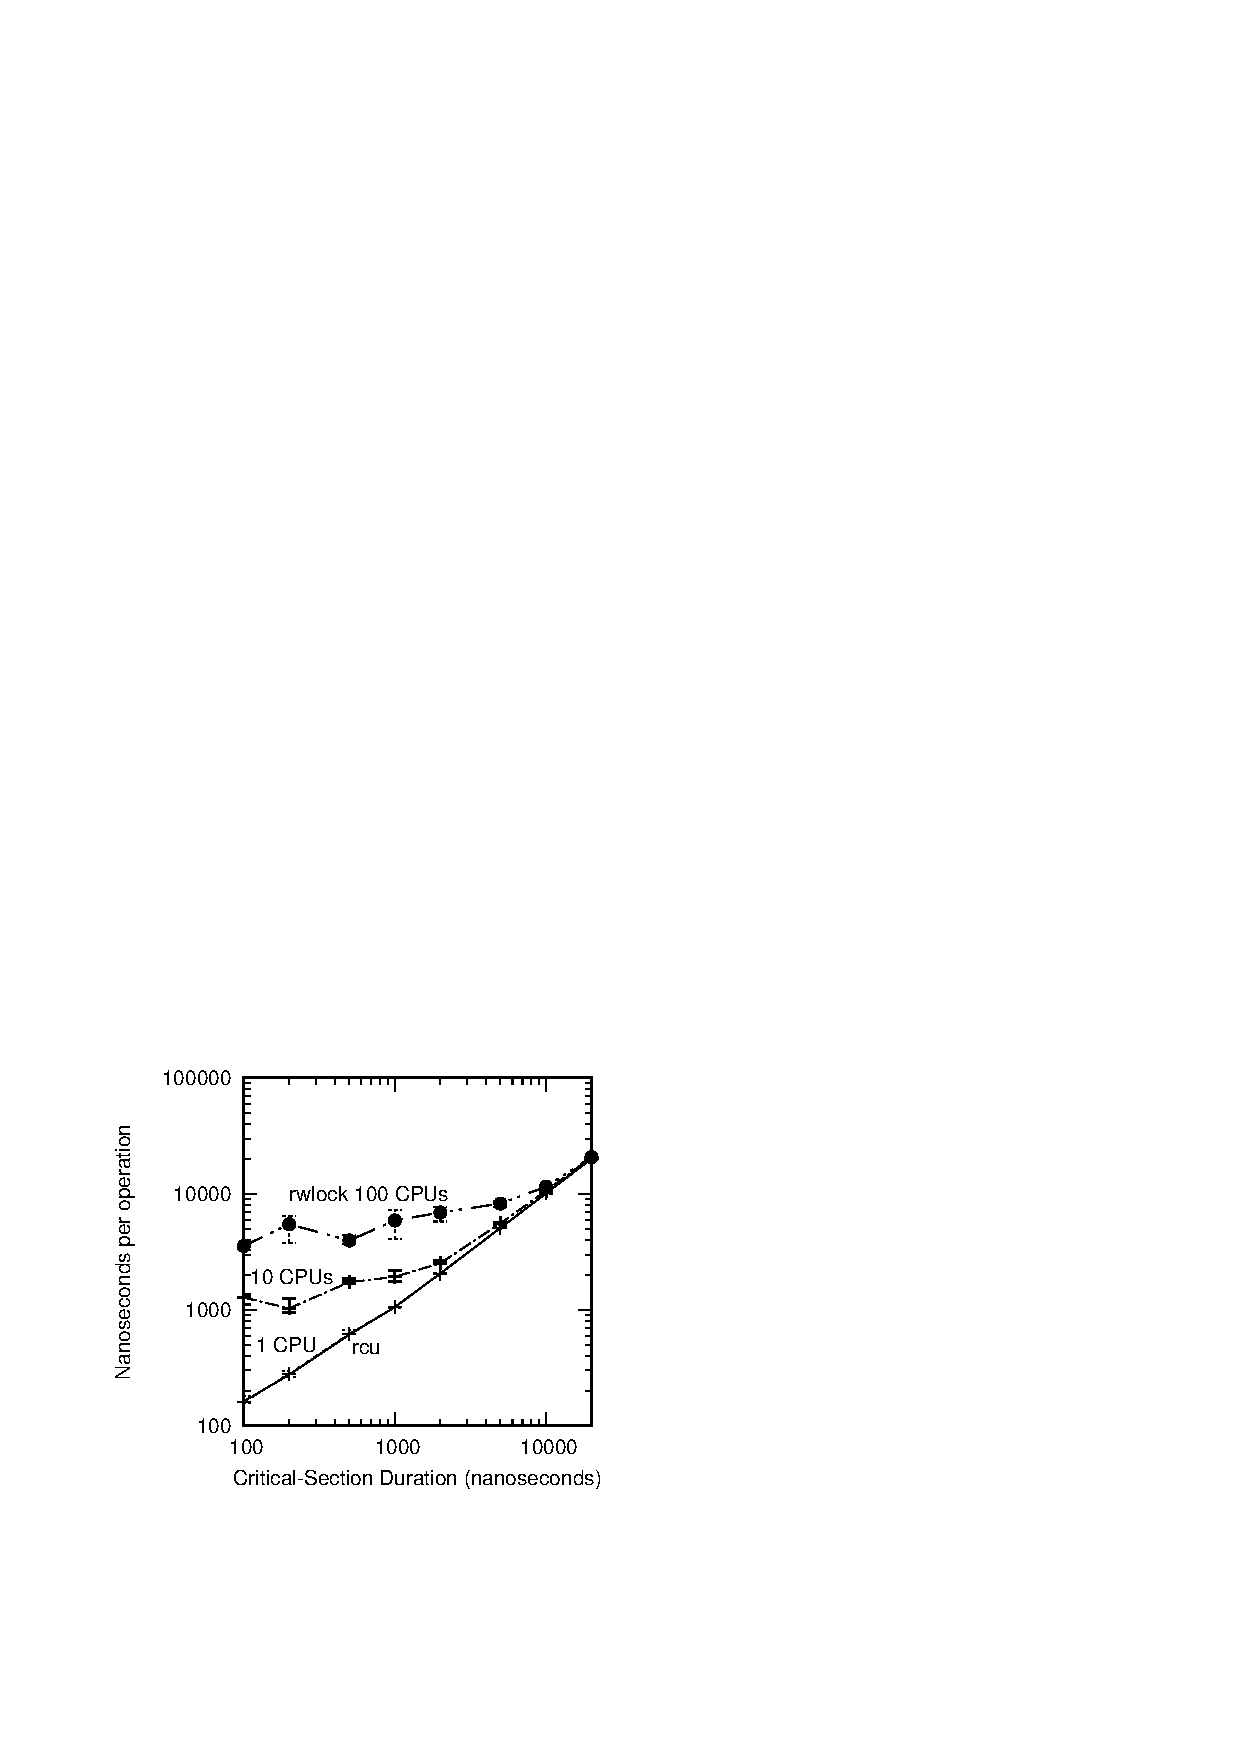
\includegraphics{defer/rwlockRCUperfwt}}
\caption{Comparison of RCU to Reader-Writer Locking as Function of Critical-Section Duration, 192 CPUs}
\label{fig:defer:Comparison of RCU to Reader-Writer Locking as Function of Critical-Section Duration}
\end{figure}

물론,
\cref{fig:defer:Performance Advantage of RCU Over Reader-Writer Locking,%
fig:defer:Performance Advantage of Preemptible RCU Over Reader-Writer Locking}
의 reader-writer 락킹의 낮은 성능은 비현실적인 0의 길이를 갖는 크리티컬 섹션에
의해 과장된 것입니다.
RCU 의 성능 이득은 크리티컬 섹션의 길이가 길어질수록 줄어듭니다.
이런 감소가 앞의 그림과 같은 시스템에서 수행된
Figure~\ref{fig:defer:Comparison of RCU to Reader-Writer Locking as Function of Critical-Section Duration}
에 보여져 있습니다.
여기서, y 축은 read-side 기능의 오버헤드와 크리티컬 섹션의 오버헤드의 합을, x
축은 크리티컬 섹션의 오버헤드를 나노세컨드 단위로 표현합니다.
하지만 y 축이 로그스케일이어서 이 그림에서의 작은 차이가 여전히 상당한 차이를
표현함을 기억해 두시기 바랍니다.
이 그림은 non-preemptible RCU 를 보입니다만, preemptible RCU 의 read-side
오버헤드가 3 나노세컨드란 점을 놓고 보면, 그 그림은
Figure~\ref{fig:defer:Comparison of RCU to Reader-Writer Locking as Function of Critical-Section Duration}
와 거의 같을 겁니다.

\iffalse

Of course, the low performance of reader-writer locking in
\cref{fig:defer:Performance Advantage of RCU Over Reader-Writer Locking,%
fig:defer:Performance Advantage of Preemptible RCU Over Reader-Writer Locking}
is exaggerated by the unrealistic zero-length critical sections.
The performance advantages of RCU decrease as the overhead of the critical
sections increase.
This decrease can be seen in
Figure~\ref{fig:defer:Comparison of RCU to Reader-Writer Locking as Function of Critical-Section Duration},
which was run on the same system as the previous plots.
Here, the y-axis represents the sum of the overhead of the read-side
primitives and that of the critical section and the x-axis represents
the critical-section overhead in nanoseconds.
But please note the logscale y~axis, which means that the small
separations between the traces still represent significant differences.
This figure shows non-preemptible RCU, but given that preemptible RCU's
read-side overhead is only about three nanoseconds, its plot would be
nearly identical to
Figure~\ref{fig:defer:Comparison of RCU to Reader-Writer Locking as Function of Critical-Section Duration}.

\fi

\QuickQuiz{
	Figure~\ref{fig:defer:Comparison of RCU to Reader-Writer Locking as Function of Critical-Section Duration}
	의 마이크로세컨드 미만 기간에서의 더 큰 에러 범위는 왜 그런거죠?

	\iffalse

	Why the larger error ranges for the submicrosecond durations in
	Figure~\ref{fig:defer:Comparison of RCU to Reader-Writer Locking as Function of Critical-Section Duration}?

	\fi

}\QuickQuizAnswer{
	더 작은 거리는 더 작은 측정에서 더 큰 상대적 에러를 초래하기
	때문입니다.
	또한, 리눅스 커널의 \co{ndelay()} 나노세컨드 단위 기능은 (2020년
	기준으로) 마이크로세컨드 이상의 시간단위 데이터를 위해 사용되는
	\co{udelay()} 보다 덜 정확합니다.
	Figure~\ref{fig:defer:Performance Advantage of RCU Over Reader-Writer Locking}
	에 보인 0 의 길이의 경우와 비교해 보는게 유익할 겁니다.

	\iffalse

	Because smaller disturbances result in greater relative errors
	for smaller measurements.
	Also, the Linux kernel's \co{ndelay()} nanosecond-scale primitive
	is (as of 2020) less accurate than is the \co{udelay()} primitive
	used for the data for durations of a microsecond or more.
	It is instructive to compare to the zero-length case shown in
	Figure~\ref{fig:defer:Performance Advantage of RCU Over Reader-Writer Locking}.

	\fi

}\QuickQuizEnd

Reader-writer 락킹을 위한 세개의 선이 있는데, 위의 것은 100~CPU, 그
다음은 10~CPU, 그리고 아래의 것은 1~CPU 에서의 것입니다.
따라서 CPU 의 수가 커지고 크리티컬 섹션이 짧아질수록 RCU 의 성능 이득은
커집니다.
이런 성능 이득은 100-CPU 시스템이 더이상 드물지 않고 여러 시스템 콜이 (그리고
그것들이 내포하는 RCU read-side 크리티컬 섹션이) 마이크로세컨드 내에 완료된다는
사실에 의해 과소평가되었습니다.

첨언하자면, 다음 문단에서 이야기 되듯, RCU read-side 기능은 거의 완전히
데드락에 내성을 가지고 있습니다.

\iffalse

There are three traces for reader-writer locking, with the upper trace
being for 100~CPUs, the next for 10~CPUs, and the lowest for 1~CPU\@.
So the greater the number of CPUs and the shorter the critical sections,
the greater is RCU's performance advantage.
These performance advantages are underscored by the fact that 100-CPU
systems are no longer uncommon and that a number of system calls (and
thus any RCU read-side critical sections that they contain) complete
within a microsecond.

In addition, as is discussed in the next paragraph,
RCU read-side primitives are almost entirely deadlock-immune.

\fi


\paragraph{Deadlock Immunity}

RCU 가 읽기가 대부분인 워크로드에 상당한 성능 이득을 제공하지만, RCU 를 만든
주요 이유는 사실 그것의 read-side 데드락 내성을 위함이었습니다.
이 내성은 RCU read-side 기능이 블록하거나 스핀하거나 뒤쪽으로 브랜칭하지 않아서
그 수행시간이 정해져있다는 사실에서 기인합니다.
따라서 그것들은 데드락 사이클에 참여될 수가 없습니다.

\iffalse

Although RCU offers significant performance advantages for
read-mostly workloads, one of the primary reasons for creating
RCU in the first place was in fact its immunity to read-side
deadlocks.
This immunity stems from the fact that
RCU read-side primitives do not block, spin, or even
do backwards branches, so that their execution time is deterministic.
It is therefore impossible for them to participate in a deadlock
cycle.

\fi

\QuickQuiz{
	이 데드락 내성에 예외가 있나요?  만약 그렇다면 어떤 이벤트들의 연속이
	데드락을 이르게 할 수 있나요?

	\iffalse

	Is there an exception to this deadlock immunity, and if so,
	what sequence of events could lead to deadlock?

	\fi

}\QuickQuizAnswer{
	RCU read-side 기능이 관여된 데드락 사이클을 만드는 한가지 방법은 다음의
	(불법적인) 선언문의 연속입니다:

	\iffalse

	One way to cause a deadlock cycle involving
	RCU read-side primitives is via the following (illegal) sequence
	of statements:

	\fi

\begin{VerbatimU}
rcu_read_lock();
synchronize_rcu();
rcu_read_unlock();
\end{VerbatimU}

	이 \co{synchronize_rcu()} 는 앞서서부터 존재한 모든 RCU read-side
	크리티컬 섹션이 완료되기 전까지 리턴할 수 없지만,
	\co{synchronize_rcu()} 가 리턴하기 전까지는 완료될 수 없는 RCU
	read-side 크리티컬 섹션에 감싸여 있습니다.
	그 결과는 고전적인 스스로에 대한 데드락입니다---reader-writer 락의
	경우에도 읽기 락을 쥐고 있는 상태에서 쓰기 락을 쥐려고 시도하면 똑같은
	결과를 얻을 겁니다.

	이 스스로에 대한 데드락 시나리오는 RCU QSBR 에 적용되지 않는데,
	\co{synchronize_rcu()} 에 의해 수행되는 컨텍스트 스위치는 이 CPU 를
	위한 quiescent state 로 동작하여 grace period 가 종료되게 할 것이기
	때문임을 알아두시기 바랍니다.
	하지만, 이는 심지어 더 나쁜 것일 뿐일텐데, 이 RCU read-side 크리티컬
	섹션에 의해 사용되는 데이터는 이 grace period 완료로 인해 메모리
	해제되었을 수도 있기 때문입니다.

	요약하자면,
	\cref{tab:defer:RCU Wait-to-Finish APIs} 에 나열된
	synchronous RCU update-side 기능을 RCU read-side 크리티컬 섹션 내에서
	사용하지 마십시오.

	\iffalse

	The \co{synchronize_rcu()} cannot return until all
	pre-existing RCU read-side critical sections complete, but
	is enclosed in an RCU read-side critical section that cannot
	complete until the \co{synchronize_rcu()} returns.
	The result is a classic self-deadlock---you get the same
	effect when attempting to write-acquire a reader-writer lock
	while read-holding it.

	Note that this self-deadlock scenario does not apply to
	RCU QSBR, because the context switch performed by the
	\co{synchronize_rcu()} would act as a quiescent state
	for this CPU, allowing a grace period to complete.
	However, this is if anything even worse, because data used
	by the RCU read-side critical section might be freed as a
	result of the grace period completing.

	In short, do not invoke synchronous RCU update-side primitives, which
	are listed in
	\cref{tab:defer:RCU Wait-to-Finish APIs},
	from within an RCU read-side critical section.

	\fi

}\QuickQuizEnd

RCU 의 read-side 데드락 내성의 한가지 흥미로운 결론은 RCU 읽기 쓰레드를
무조건적으로 RCU 업데이트 쓰레드로 업그레이드 할 수 있다는 것입니다.
Reader-writer 락킹에서 그런 업그레이드를 시도하는 것은 데드락을 초래합니다.
RCU read-to-update 업그레이드를 하는 코드 조각은 다음과 같을겁니다:

\iffalse

An interesting consequence of RCU's read-side deadlock immunity is
that it is possible to unconditionally upgrade an RCU
reader to an RCU updater.
Attempting to do such an upgrade with reader-writer locking results
in deadlock.
A sample code fragment that does an RCU read-to-update upgrade follows:

\fi

\begin{VerbatimN}[samepage=true]
rcu_read_lock();
list_for_each_entry_rcu(p, &head, list_field) {
	do_something_with(p);
	if (need_update(p)) {
		spin_lock(my_lock);
		do_update(p);
		spin_unlock(&my_lock);
	}
}
rcu_read_unlock();
\end{VerbatimN}

\co{do_update()} 는 락의 보호, \emph{그리고} RCU read-side 보호 아래 수행됨에
주의하십시오.

RCU 의 데드락 내성의 또다른 흥미로운 결론은 커다란 범주의 우선순위 역전 문제에
대한 내성입니다.
예를 들어, 낮은 우선순위 RCU 읽기 쓰레드가 높은 우선순위 RCU 업데이트 쓰레드가
update-side 락을 잡는걸 방지하지 못합니다.
비슷하게, 낮은 우선순위 RCU 업데이트 쓰레드는 높은 우선순위 RCU 읽기 쓰레드가
RCU read-side 크리티컬 섹션에 들어가는 것을 막지 못합니다.

\iffalse

Note that \co{do_update()} is executed under
the protection of the lock \emph{and} under RCU read-side protection.

Another interesting consequence of RCU's deadlock immunity is its
immunity to a large class of priority inversion problems.
For example, low-priority RCU readers cannot prevent a high-priority
RCU updater from acquiring the update-side lock.
Similarly, a low-priority RCU updater cannot prevent high-priority
RCU readers from entering an RCU read-side critical section.

\fi

\QuickQuiz{
	데드락과 우선순위 역전에 모두 내성이 있다???
	사실이라기엔 너무 좋아보이는데요.
	이게 가능하다는 걸 제가 왜 믿어야 하죠?

	\iffalse

	Immunity to both deadlock and priority inversion???
	Sounds too good to be true.
	Why should I believe that this is even possible?

	\fi

}\QuickQuizAnswer{
	진짜 동작합니다.
	어쨌건, 그렇지 않다면 리눅스 커널은 동작하지 못할겁니다.

	\iffalse

	It really does work.
	After all, if it didn't work, the Linux kernel would not run.

	\fi

}\QuickQuizEnd

\paragraph{Realtime Latency}

RCU read-side 기능들은 스핀하지도 블록하지도 않기 때문에, 훌륭한 realtime
반응시간을 제공합니다.
추가적으로, 앞에서도 이야기 했듯 이는 RCU read-side 기능들과 락이 연관된
우선순위 역전 문제에 내성이 있음을 의미합니다.

하지만, RCU 는 더 복잡한 우선순위 역전 시나리오에는 문제가 있을 수 있는데, 예를
들면 높은 우선순위의 프로세스는 낮은 우선순위의 RCU 읽기 쓰레드에 의해 \rt\
커널에서 한 RCU grace period 가 지나갈 때까지 블록될 수 있습니다.
이는 RCU 우선순위 부스팅을 통해 해결될 수
있습니다~\cite{PaulEMcKenney2007BoostRCU,DinakarGuniguntala2008IBMSysJ}.

\iffalse

Because RCU read-side primitives neither spin nor block, they offer
excellent realtime latencies.
In addition, as noted earlier, this means that they are
immune to priority inversion
involving the RCU read-side primitives and locks.

However, RCU is susceptible to more subtle priority-inversion scenarios,
for example, a high-priority process blocked waiting for an RCU
grace period to elapse can be blocked by low-priority RCU readers
in \rt\ kernels.
This can be solved by using RCU priority
boosting~\cite{PaulEMcKenney2007BoostRCU,DinakarGuniguntala2008IBMSysJ}.

\fi

\paragraph{RCU Readers and Updaters Run Concurrently}

RCU 읽기 쓰레드는 스핀도 블록도 하지 않으므로, 그리고 업데이트 쓰레드는 어떤
종류의 롤백이나 abort 도 하지 않으므로, RCU 읽기 쓰레드와 업데이트 쓰레드는
동시에 수행되어야만 합니다.
이는 RCU 읽기 쓰레드가 오래되어 더이상 유효하지 않은 데이터를 읽을수도 있고,
비일관적인 모습을 보게 될수도 있음을, 따라서 reader-writer 락킹에서 RCU 로의
전환에 혼란을 야기할 수 있음을 의미합니다.

\iffalse

Because RCU readers never spin nor block, and because updaters are not
subject to any sort of rollback or abort semantics, RCU readers and
updaters must necessarily run concurrently.
This means that RCU readers might access stale data, and might even
see inconsistencies, either of which can render conversion from reader-writer
locking to RCU non-trivial.

\fi

\begin{figure}[tb]
\centering
\resizebox{3in}{!}{\includegraphics{defer/rwlockRCUupdate}}
\caption{Response Time of RCU vs. Reader-Writer Locking}
\label{fig:defer:Response Time of RCU vs. Reader-Writer Locking}
\end{figure}

하지만, 놀라우리만치 많은 상황에서 비일관성과 오래되어 더이상 유효하지 않은
데이터는 문제가 되지 않습니다.
고전적인 예는 네트워킹 라우팅 테이블입니다.
라우팅 업데이트는 특정 시스템까지 닿는데 상당한 시간을 요하므로 (수초에서
수분까지도), 시스템은 이 업데이트가 도착하기 전까지 상당한 시간동안 패킷을
잘못된 방향으로 보낼 수 있습니다.
업데이트를 몇 추가적인 밀리세컨드 동안 잘못된 방향으로 보내는 건 보통 문제가
아닙니다.
더 나아가, RCU 업데이트 쓰레드는 RCU 읽기 쓰레드가 끝나기를 기다리지 않고
변화를 만들 수 있으므로, RCU 읽기 쓰레드는
Figure~\ref{fig:defer:Response Time of RCU vs. Reader-Writer Locking}
에 보인 것처럼 batch-fair reader-writer 락킹의 읽기 쓰레드보다 빠르게 변화를 볼
수도 있습니다.

\iffalse

However, in a surprisingly large number of situations, inconsistencies and
stale data are not problems.
The classic example is the networking routing table.
Because routing updates can take considerable time to reach a given
system (seconds or even minutes), the system will have been sending
packets the wrong way for quite some time when the update arrives.
It is usually not a problem to continue sending updates the wrong
way for a few additional milliseconds.
Furthermore, because RCU updaters can make changes without waiting for
RCU readers to finish,
the RCU readers might well see the change more quickly than would
batch-fair
reader-writer-locking readers, as shown in
Figure~\ref{fig:defer:Response Time of RCU vs. Reader-Writer Locking}.

\fi

일단 업데이트가 도달하면, rwlock 쓰기 쓰레드는 마지막 읽기 쓰레드가 완료되기
전까지 진행될 수 없으며, 뒤따르는 읽기 쓰레드는 이 쓰기 쓰레드가 완료되기
전까지 진행될 수 없습니다.
하지만, 이 뒤따르는 읽기 쓰레드는 오른쪽 상자의 초록색으로 표시되었듯 이 새
값을 읽을 수 있는게 보장됩니다.
대조적으로, RCU 읽기 쓰레드와 업데이트 쓰레드는 서로를 블록할 수 없어서, RCU
읽기 쓰레드가 이 업데이트된 값을 더 빨리 볼 수 있게 합니다.
물론, 이것들의 수행이 RCU 업데이트 쓰레드의 그것과 겹치므로, \emph{모든} RCU
읽기 쓰레드는 업데이트된 값을 읽을 수도 있는데, 이 업데이트 전부터 시작된
세개의 읽기 쓰레드 역시 포함됩니다.
하지만 초록색으로 칠해진 가장 오른쪽 RCU 읽기 쓰레드만이 업데이트된 값을 볼
것으로 \emph{보장됩니다}.

Reader-writer 락킹과 RCU 는 그저 다른 보장을 제공할 뿐입니다.
Reader-writer 락킹에서 어떤 쓰기 쓰레드의 시작보다 나중에 시작된 읽기 쓰레드는
새 값을 볼 것이 보장되고, 이 쓰레드가 스핀하고 있는 사이 시작되려 하는 읽기
쓰레드는 새 값을 볼수도 보지 못할 수도 있는데, 사용되는 rwlock 구현의 읽기/쓰기
쓰레드 선호도에 의존적입니다.
대조적으로, RCU 에서 업데이트 쓰레드가 완료되기 전에 시작된 모든 읽기 쓰레드는
새 값을 볼 것이 보장되며, 업데이트 쓰레드가 시작한 후에 완료된 모든 읽기
쓰레드는 타이밍에 따라 새 값을 볼 수도 보지 못할 수도 있습니다.

\iffalse

Once the update is received, the rwlock writer cannot proceed until the
last reader completes, and subsequent readers cannot proceed until the
writer completes.
However, these subsequent readers are guaranteed to see the new value,
as indicated by the green shading of the rightmost boxes.
In contrast, RCU readers and updaters do not block each other, which permits
the RCU readers to see the updated values sooner.
Of course, because their execution overlaps that of the RCU updater,
\emph{all} of the RCU readers might well see updated values, including
the three readers that started before the update.
Nevertheless only the green-shaded rightmost RCU readers
are \emph{guaranteed} to see the updated values.

Reader-writer locking and RCU simply provide different guarantees.
With reader-writer locking, any reader that begins after the writer begins
is guaranteed to see new values, and any reader that attempts to
begin while the writer is spinning might or might not see new values,
depending on the reader/writer preference of the rwlock implementation in
question.
In contrast, with RCU, any reader that begins after the updater completes
is guaranteed to see new values, and any reader that completes after the
updater begins might or might not see new values, depending on timing.

\fi

여기서의 핵심은 reader-writer 락킹이 컴퓨터 시스템 내에서는 일관성을 실제로
보장하지만, 이 일관성이 바깥 세상의 \emph{비일관성} 의 증가를 대가로 오는
경우가 존재한다는 것입니다.
달리 말하자면 reader-writer 락킹은 바깥 세상 관점에서 조용하게 오래되어
유효하지 않아진 데이터를 대가로 내부적 일관성을 획득합니다.

그러나, 시스템 내에서의 비일관성과 오래되어 유효하지 않아진 데이터가 제어되지
못하는 상황도 있습니다.
다행히, 비일관성과 오래되어 유효하지 않아진 데이터를 막는 여러 방법이
존재하며~\cite{PaulEdwardMcKenneyPhD,Arcangeli03}, 레퍼런스 카운팅에 기반한
일부 방법이 Section~\ref{sec:defer:Reference Counting} 에서 다루어집니다.

\iffalse

The key point here is that, although reader-writer locking does
indeed guarantee consistency within the confines of the computer system,
there are situations where this consistency comes at the price of
increased \emph{inconsistency} with the outside world.
In other words, reader-writer locking obtains internal consistency at the
price of silently stale data with respect to the outside world.

Nevertheless, there are situations where inconsistency and stale
data within the confines of the system cannot be tolerated.
Fortunately,
there are a number of approaches that avoid inconsistency and stale
data~\cite{PaulEdwardMcKenneyPhD,Arcangeli03}, and some
methods based on reference counting are discussed in
Section~\ref{sec:defer:Reference Counting}.

\fi

\paragraph{Low-Priority RCU Readers Can Block High-Priority Reclaimers}

Realtime RCU~\cite{DinakarGuniguntala2008IBMSysJ} 또는
SRCU~\cite{PaulEMcKenney2006c} 에서, preemption 당한 읽기 쓰레드는 grace period
가 완료되는 것을 막을 것인데, 심지어 높은 우선순위 작업이 그 grace period
완료를 기다리며 블록되어 있더라도 그렇습니다.
Realtime RCU 는 \co{call_rcu()} 로 \co{synchronize_rcu()} 를 대체하거나 RCU
우선순위 부스팅을
이용해~\cite{PaulEMcKenney2007BoostRCU,DinakarGuniguntala2008IBMSysJ} 이를 막을
수 있는데, 2008년 초 기준으로 아직 실험적 상태입니다.
SRCU 와 QRCU 를 우선순위 부스팅과 결합시키는게 필요해질 수도 있지만, 분명한
실제 세계에서의 필요가 확인되기 전까지는 아닙니다.

\iffalse

In Realtime RCU~\cite{DinakarGuniguntala2008IBMSysJ} or
SRCU~\cite{PaulEMcKenney2006c},
a preempted reader will prevent a grace period from completing, even if
a high-priority task is blocked waiting for that grace period to complete.
Realtime RCU can avoid this problem by substituting \co{call_rcu()}
for \co{synchronize_rcu()} or by using RCU priority
boosting~\cite{PaulEMcKenney2007BoostRCU,DinakarGuniguntala2008IBMSysJ},
which is still in experimental status as of early 2008.
It might become necessary to augment SRCU and QRCU with priority boosting,
but not before a clear real-world need is demonstrated.

\fi

\paragraph{RCU Grace Periods Extend for Many Milliseconds}

Userspace RCU~\cite{MathieuDesnoyers2009URCU,PaulMcKenney2013LWNURCU}, 가속된
grace period, 그리고
Appendix~\ref{chp:app:``Toy'' RCU Implementations} 에 이야기 된 여러 ``장난감''
RCU 구현들의 예외가 있지만, RCU grace period 는 수 밀리세컨드까지 늘어날 수
있습니다.
가능한 곳에 비동기 인터페이스를 (\co{call_rcu()} 와 \co{call_rcu_bh()})
사용하는 것을 포함해 그런 오랜 지연을 문제가 되지 않게 하는 여러 기법이
존재하지만 이는 RCU 가 읽기가 대부분인 상황에서 사용되는 관습적 규칙의 주요
이유 중 하나입니다.

\iffalse

With the exception of userspace
RCU~\cite{MathieuDesnoyers2009URCU,PaulMcKenney2013LWNURCU},
expedited grace periods, and several of the ``toy''
RCU implementations described in
Appendix~\ref{chp:app:``Toy'' RCU Implementations},
RCU grace periods extend milliseconds.
Although there are a number of techniques to render such long delays
harmless, including use of the asynchronous interfaces where available
(\co{call_rcu()} and \co{call_rcu_bh()}), this situation
is a major reason for the rule of thumb that RCU be used in read-mostly
situations.

\fi

\paragraph{Code: Reader-Writer Locking vs. RCU Code}

최선의 경우, reader-writer 락킹에서 RCU 로의 전환은
Listing~\ref{lst:defer:Converting Reader-Writer Locking to RCU: Data},
\ref{lst:defer:Converting Reader-Writer Locking to RCU: Search},
그리고
\ref{lst:defer:Converting Reader-Writer Locking to RCU: Deletion}
에 보인 것처럼 상당히 단순할 수 있는데, 이것들은 모두
Wikipedia~\cite{WikipediaRCU} 에서 가져온 것들입니다.

\iffalse


In the best case, the conversion from reader-writer locking to RCU
is quite simple, as shown in
Listings~\ref{lst:defer:Converting Reader-Writer Locking to RCU: Data},
\ref{lst:defer:Converting Reader-Writer Locking to RCU: Search},
and
\ref{lst:defer:Converting Reader-Writer Locking to RCU: Deletion},
all taken from
Wikipedia~\cite{WikipediaRCU}.

\fi

\begin{listing*}[htbp]
{ \scriptsize
\begin{verbbox}
 1 struct el {                           1 struct el {
 2   struct list_head lp;                2   struct list_head lp;
 3   long key;                           3   long key;
 4   spinlock_t mutex;                   4   spinlock_t mutex;
 5   int data;                           5   int data;
 6   /* Other data fields */             6   /* Other data fields */
 7 };                                    7 };
 8 DEFINE_RWLOCK(listmutex);             8 DEFINE_SPINLOCK(listmutex);
 9 LIST_HEAD(head);                      9 LIST_HEAD(head);
\end{verbbox}
}
\hspace*{0.9in}\OneColumnHSpace{-0.5in}
\theverbbox
\caption{Converting Reader-Writer Locking to RCU: Data}
\label{lst:defer:Converting Reader-Writer Locking to RCU: Data}
\end{listing*}

\begin{listing*}[htbp]
{ \scriptsize
\begin{verbbox}
 1 int search(long key, int *result)     1 int search(long key, int *result)
 2 {                                     2 {
 3   struct el *p;                       3   struct el *p;
 4                                       4
 5   read_lock(&listmutex);              5   rcu_read_lock();
 6   list_for_each_entry(p, &head, lp) { 6   list_for_each_entry_rcu(p, &head, lp) {
 7     if (p->key == key) {              7     if (p->key == key) {
 8       *result = p->data;              8       *result = p->data;
 9       read_unlock(&listmutex);        9       rcu_read_unlock();
10       return 1;                      10       return 1;
11     }                                11     }
12   }                                  12   }
13   read_unlock(&listmutex);           13   rcu_read_unlock();
14   return 0;                          14   return 0;
15 }                                    15 }
\end{verbbox}
}
\hspace*{0.9in}\OneColumnHSpace{-0.5in}
\theverbbox
\caption{Converting Reader-Writer Locking to RCU: Search}
\label{lst:defer:Converting Reader-Writer Locking to RCU: Search}
\end{listing*}

\begin{listing*}[htbp]
{ \scriptsize
\begin{verbbox}
 1 int delete(long key)                  1 int delete(long key)
 2 {                                     2 {
 3   struct el *p;                       3   struct el *p;
 4                                       4
 5   write_lock(&listmutex);             5   spin_lock(&listmutex);
 6   list_for_each_entry(p, &head, lp) { 6   list_for_each_entry(p, &head, lp) {
 7     if (p->key == key) {              7     if (p->key == key) {
 8       list_del(&p->lp);               8       list_del_rcu(&p->lp);
 9       write_unlock(&listmutex);       9       spin_unlock(&listmutex);
                                        10       synchronize_rcu();
10       kfree(p);                      11       kfree(p);
11       return 1;                      12       return 1;
12     }                                13     }
13   }                                  14   }
14   write_unlock(&listmutex);          15   spin_unlock(&listmutex);
15   return 0;                          16   return 0;
16 }                                    17 }
\end{verbbox}
}
\hspace*{0.9in}\OneColumnHSpace{-0.5in}
\theverbbox
\caption{Converting Reader-Writer Locking to RCU: Deletion}
\label{lst:defer:Converting Reader-Writer Locking to RCU: Deletion}
\end{listing*}

하지만, 이런 전환이 항상 단순하지는 않습니다.
이는
\cref{lst:defer:Converting Reader-Writer Locking to RCU: Deletion}
의 \co{spin_lock()} 도 \co{synchronize_rcu()} 도
\cref{lst:defer:Converting Reader-Writer Locking to RCU: Search}
의 읽기 쓰레드를 배제시키지 않기 때문입니다.
첫째로, \co{spin_lock()} 은 \co{rcu_read_lock()} 과 \co{rcu_read_unlock()} 과
상호작용하지 않으며 따라서 그것들을 배제하지 않습니다.
둘째로, \co{write_lock()} 과 \co{synchronize_rcu()} 가 앞서서부터 존재한 읽기
쓰레드를 기다리지만 \co{write_lock()} 만이 뒤따르는 읽기 쓰레드의 시작을
방지합니다.\footnote{
	누구였든 이걸 Paul 에게 지적해준 분에게 감사를.}
따라서, \co{synchronize_rcu()} 는 읽기 쓰레드를 배제하지 못합니다.
따라서 reader-writer 락킹을 사용하는 많은 상황이 RCU 로 쉽게 바뀔 수 있다는
사실은 놀랍습니다.

Reader-writer 락킹을 RCU 로 교체하는 더 자세한 경우들이 다른 곳에서도 발견될 수
있을 겁니다~\cite{NeilBrown2015PathnameLookup,NeilBrown2015RCUwalk}.

\iffalse

However, the transformation is not always this straightforward.
This is because neither the \co{spin_lock()} nor the
\co{synchronize_rcu()} in
\cref{lst:defer:Converting Reader-Writer Locking to RCU: Deletion}
exclude the readers in
\cref{lst:defer:Converting Reader-Writer Locking to RCU: Search}.
First, the \co{spin_lock()} does not interact in any way with
\co{rcu_read_lock()} and \co{rcu_read_unlock()}, thus not excluding them.
Second, although both \co{write_lock()} and \co{synchronize_rcu()}
wait for pre-existing readers, only \co{write_lock()} prevents
subsequent readers from commencing.\footnote{
	Kudos to whoever pointed this out to Paul.}
Thus, \co{synchronize_rcu()} cannot exclude readers.
It is therefore surprising that a great many situations
using reader-writer locking can be easily converted to RCU\@.

More-elaborate cases of replacing reader-writer locking with RCU
may be found
elsewhere~\cite{NeilBrown2015PathnameLookup,NeilBrown2015RCUwalk}.

\fi

\paragraph{Semantics: Reader-Writer Locking vs. RCU Semantics}

Reader-writer 락킹 semantic 은 거칠고 비정규적으로 다음의 세가지 임시적 제약으로
요약될 수 있습니다:

\begin{enumerate}
\item	쓰기 락 획득은 모든 읽기 락을 잡은 쓰레드들이 그 락을 놓기를
	기다립니다.
\item	쓰기 락 획득은 모든 쓰기 락을 잡은 쓰레드들이 그 락을 놓기를
	기다립니다.
\item	읽기 락 획득은 모든 쓰기 락을 잡은 쓰레드들이 그 락을 놓기를
	기다립니다.
\end{enumerate}

\iffalse

Reader-writer locking semantics can be roughly and informally summarized
by the following three temporal constraints:

\begin{enumerate}
\item	Write-side acquisitions wait for any read-holders to release
	the lock.
\item	Writer-side acquisitions wait for any write-holder to release
	the lock.
\item	Read-side acquisitions wait for any write-holder to release
	the lock.
\end{enumerate}

\fi

RCU 는 제약~\#3 을 완전히 사라지게 하고 나머지 두개도 다음과 같이 완화시킵니다:

\begin{enumerate}
\item	쓰기 쓰레드는 모든 앞서서부터 존재해온 읽기 락을 잡은 쓰레드들을
	업데이트의 파괴적인 단계를 (일반적으로 메모리 해제) 처리하기 전에
	기다립니다.
\item	쓰기 쓰레드는 서로간에 필요한 바에 맞춰 동기화 합니다.
\end{enumerate}

물론 이 완화가 RCU 구현이 훌륭한 성능과 확장성을 얻을 수 있게 합니다.
RCU 사용처들은 이 완화를 놀랄만큼 많은 방법으로 보상합니다만 일반적으로 공간적
제약을 사용합니다:

\begin{enumerate}
\item	새 데이터는 새로 할당된 메모리에 위치합니다.
\item	오래된 데이터는 메모리 해제되지만, 다음의 조건이 충족된 후에만 합니다:
	\begin{enumerate}
	\item	데이터가 뒤의 읽기 쓰레드에 의해선 접근 불가능하게끔 링크
		삭제되었을 것, 그리고
	\item	뒤따르는 RCU grace period 가 지났을 것.
	\end{enumerate}
\end{enumerate}

\iffalse

RCU dispenses entirely with constraint~\#3 and weakens the other two
as follows:

\begin{enumerate}
\item	Writers wait for any pre-existing read-holders before progressing
	to the destructive phase of their update (usually the freeing of
	memory).
\item	Writers synchronize with each other as needed.
\end{enumerate}

It is of course this weakening that permits RCU implementations to attain
excellent performance and scalability.
RCU use cases compensate for this weakening in a surprisingly large number
of ways, but most commonly by imposing spatial constraints:

\begin{enumerate}
\item	New data is placed in newly allocated memory.
\item	Old data is freed, but only after:
	\begin{enumerate}
	\item	That data has been unlinked so as to be inaccessible
		to later readers, and
	\item	A subsequent RCU grace period has elapsed.
	\end{enumerate}
\end{enumerate}

\fi

요약해서, RCU 는 자신의 쓰기 성능과 확장성을 시공간적 제약에 기반한 semantic 을
통해 얻습니다.

\iffalse

In short, RCU attains its read-side performance and scalability by
constructing semantics based on combined temporal and spatial constraints.

\fi

\subsubsection{RCU is a Restricted Reference-Counting Mechanism}
\label{sec:defer:RCU is a Restricted Reference-Counting Mechanism}

Grace period 는 진행중인 RCU read-side 크리티컬 섹션이 있는 동안은 완료될 수
없으므로, RCU read-side 기능들은 제한된 레퍼런스 카운팅 메커니즘으로 사용될 수
있습니다.
예를 들어, 다음 코드 조각을 생각해 봅시다:

\iffalse

Because grace periods are not allowed to complete while
there is an RCU read-side critical section in progress,
the RCU read-side primitives may be used as a restricted
reference-counting mechanism.
For example, consider the following code fragment:

\fi

\begin{VerbatimN}
rcu_read_lock();  /* acquire reference. */
p = rcu_dereference(head);
/* do something with p. */
rcu_read_unlock();  /* release reference. */
\end{VerbatimN}

\co{rcu_read_lock()} 기능은 \co{p} 로의 레퍼런스를 얻는 것으로 생각될 수도
있는데, \co{rcu_dereference()} 가 \co{p} 에 값을 할당한 뒤에 시작되는 grace
period 는 우리가 매칭되는 \co{rcu_read_unlock()} 전까지는 종료될 수 없기
때문입니다.
이 레퍼런스 카운팅 방법은 우리가 RCU read-side 크리티컬 섹션 내에서는 블록될 수
없으며 RCU read-side 크리티컬 섹션을 한 태스크에서 다른 태스크로 넘길 수도
없다는 사실로 제약이 됩니다.

이런 제약과 무관하게, 다음 코드는 안전하게 \co{p} 를 삭제합니다:

\iffalse

The \co{rcu_read_lock()} primitive can be thought of as
acquiring a reference to \co{p}, because a grace period
starting after the \co{rcu_dereference()} assigns to \co{p}
cannot possibly end until after we reach the matching
\co{rcu_read_unlock()}.
This reference-counting scheme is restricted in that
we are not allowed to block in RCU read-side critical sections,
nor are we permitted to hand off an RCU read-side critical section
from one task to another.

Regardless of these restrictions,
the following code can safely delete \co{p}:

\fi

\begin{VerbatimN}
spin_lock(&mylock);
p = head;
rcu_assign_pointer(head, NULL);
spin_unlock(&mylock);
/* Wait for all references to be released. */
synchronize_rcu();
kfree(p);
\end{VerbatimN}

\co{head} 로의 할당은 미래의 \co{p} 로의 레퍼런스가 얻어지는 것을 방지하고,
\co{synchronize_rcu()} 는 모든 앞서 획득된 레퍼런스가 해제되기를 기다립니다.

\iffalse

The assignment to \co{head} prevents any future references
to \co{p} from being acquired, and the \co{synchronize_rcu()}
waits for any previously acquired references to be released.

\fi

\QuickQuiz{
	하지만 잠시만요!
	이건 RCU 를 reader-writer 락킹의 대체제로 생각할 때 사용될 수 있는 것과
	완전히 똑같은 코드예요!
	뭐죠?

	\iffalse

	But wait!
	This is exactly the same code that might be used when thinking
	of RCU as a replacement for reader-writer locking!
	What gives?

	\fi

}\QuickQuizAnswer{
	이건 장난감 예제의 법칙의 효과입니다:
	어떤 지점 이후부터는 코드 조각들은 똑같이 보입니다.
	유일한 차이점은 우리가 그 코드를 어떻게 생각하느냐에 있습니다.
	하지만, 이 차이점은 무척 중요할 수 있습니다.
	그 중요성에 대해 한가지만 예를 들어보자면, 우리가 RCU 를 제한된
	레퍼런스 카운팅 방법으로 생각한다면, 우린 업데이트가 RCU read-side
	크리티컬 섹션을 배제시킬 거라는 바보스러운 생각에 빠지진 않을 겁니다.

	그러나 RCU 를 reader-writer 락킹의 대체제로 생각하는 것도 종종
	유용한데, 예를 들면 reader-writer 락킹을 RCU 로 대체할 때 그렇습니다.

	\iffalse

	This is an effect of the Law of Toy Examples:
	beyond a certain point, the code fragments look the same.
	The only difference is in how we think about the code.
	However, this difference can be extremely important.
	For but one example of the importance, consider that if we think
	of RCU as a restricted reference counting scheme, we would never
	be fooled into thinking that the updates would exclude the RCU
	read-side critical sections.

	It nevertheless is often useful to think of RCU as a replacement
	for reader-writer locking, for example, when you are replacing
	reader-writer locking with RCU\@.

	\fi

}\QuickQuizEnd

물론, RCU 는
Section~\ref{sec:together:Refurbish Reference Counting}
에서 이야기 된 것처럼 전통적인 레퍼런스 카운팅과 결합될 수도 있습니다.

\iffalse

Of course, RCU can also be combined with traditional reference counting,
as discussed in
Section~\ref{sec:together:Refurbish Reference Counting}.

\fi

\begin{figure}[tb]
\centering
\resizebox{2.5in}{!}{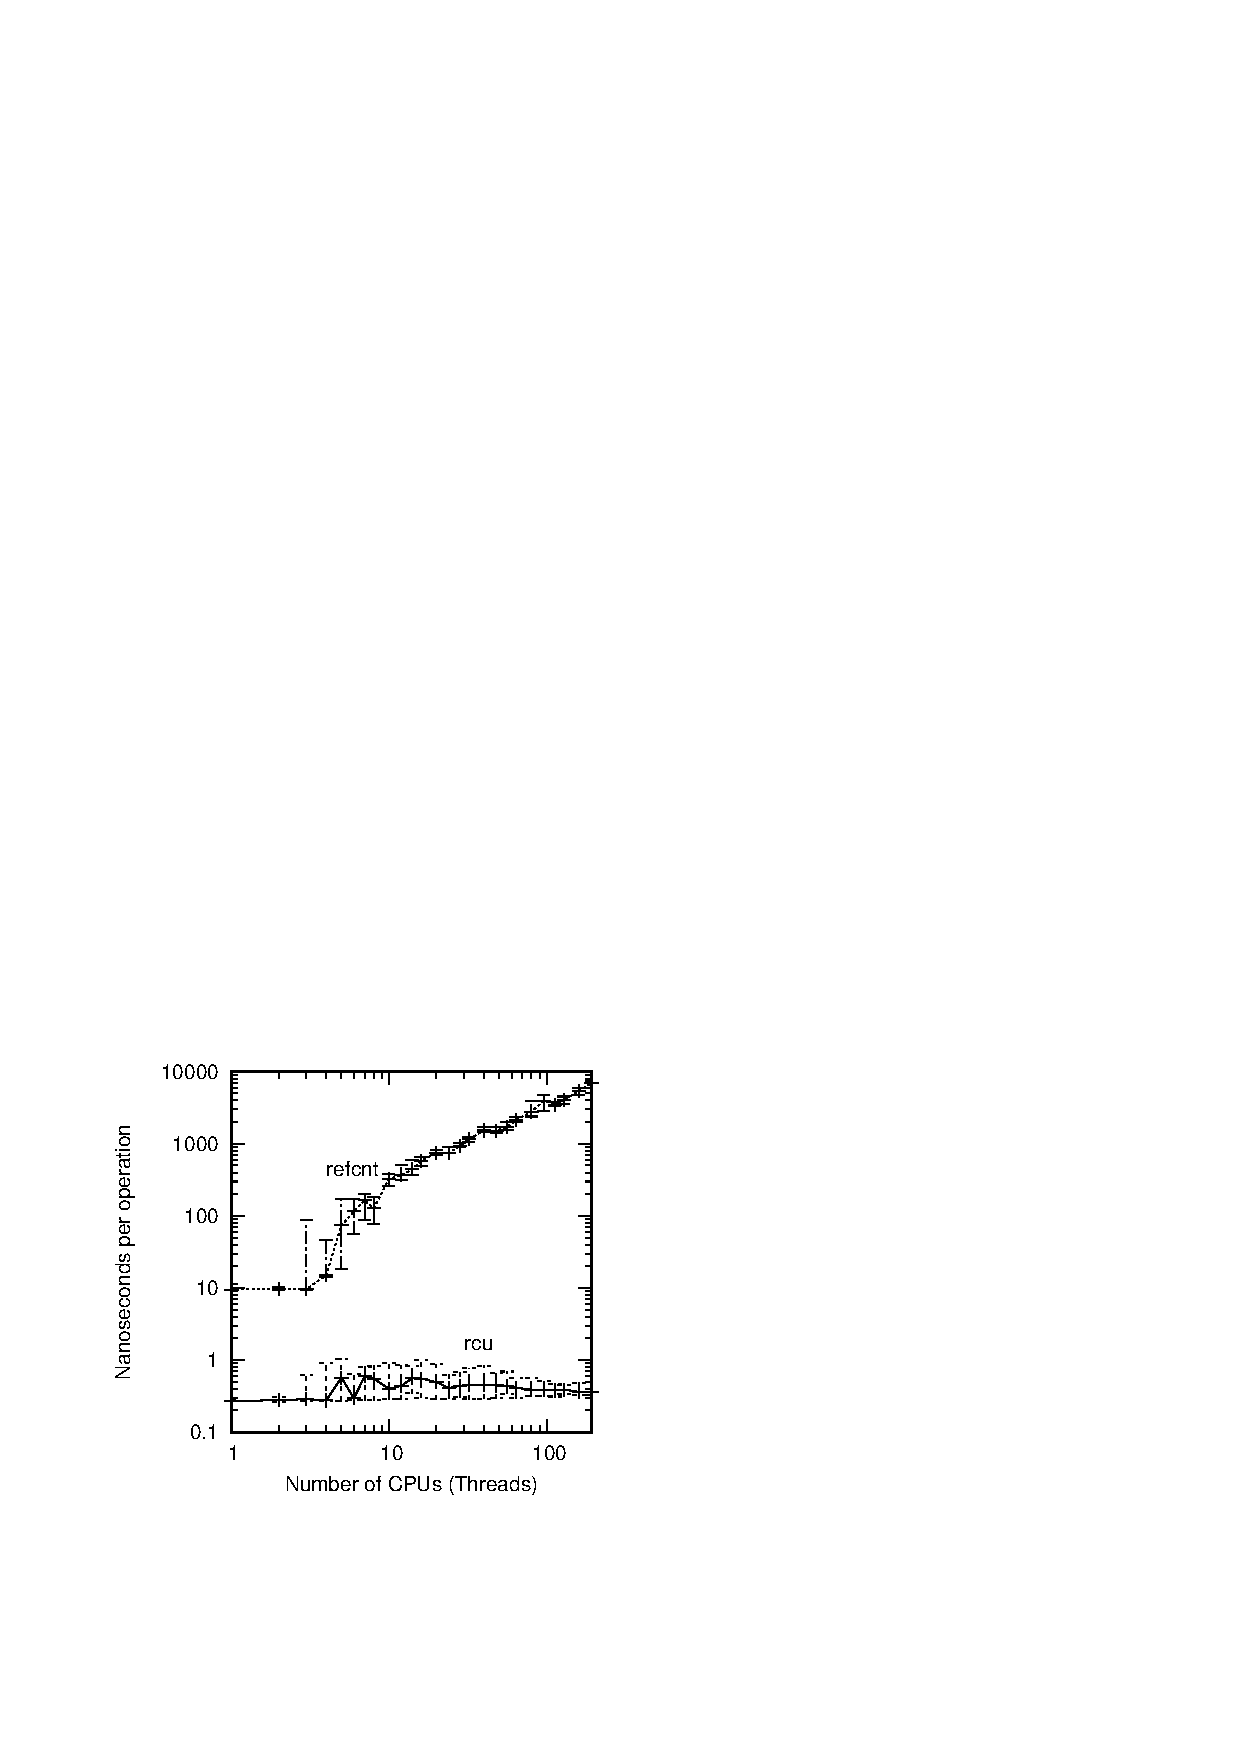
\includegraphics{defer/refcntRCUperf}}
\caption{Performance of RCU vs. Reference Counting}
\label{fig:defer:Performance of RCU vs. Reference Counting}
\end{figure}

\begin{figure}[tb]
\centering
\resizebox{2.5in}{!}{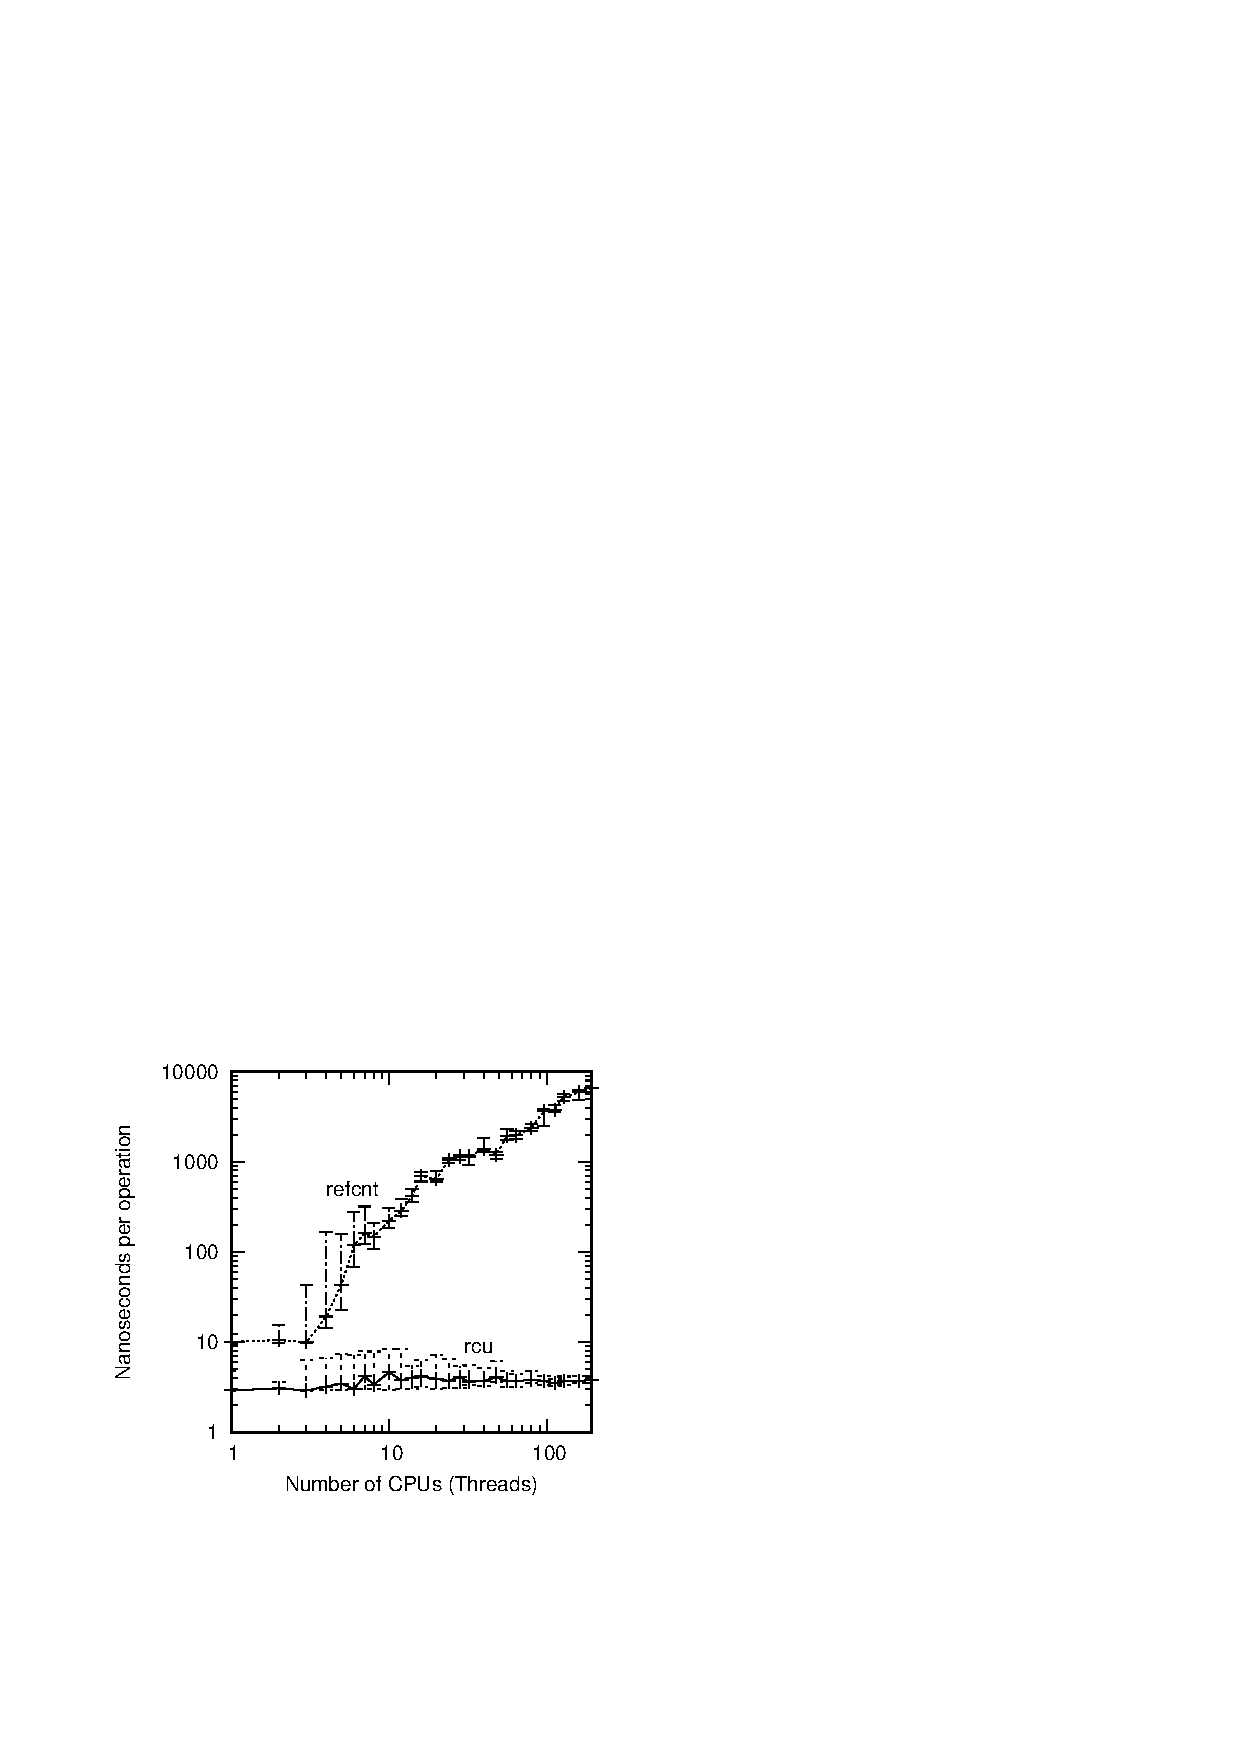
\includegraphics{defer/refRCUperfPREEMPT}}
\caption{Performance of Preemptible RCU vs. Reference Counting}
\label{fig:defer:Performance of Preemptible RCU vs. Reference Counting}
\end{figure}

그런데 이걸 왜 신경씁니까?
다시 말하지만, 답은 성능으로, 448-CPU 2.1\,GHz Intel x86 시스템에서
non-preemptible 과 preemtible 리눅스 커널 RCU 를 사용해 각각 얻어진
Figure~\ref{fig:defer:Performance of RCU vs. Reference Counting}
와~\ref{fig:defer:Performance of Preemptible RCU vs. Reference Counting}
에서 보인 것과 같습니다.
Non-preemptible RCU 의 레퍼런스 카운팅 대비 장점은 단일 CPU 에서 수십배를
넘으며 192~CPU 에서는 수만배까지 달합니다.
Preemptible RCU 의 장점은 단일 CPU 에서 약 세배에서 192~CPU 에서 수천배까지
이릅니다.

\iffalse

But why bother?
Again, part of the answer is performance, as shown in
Figures~\ref{fig:defer:Performance of RCU vs. Reference Counting}
and~\ref{fig:defer:Performance of Preemptible RCU vs. Reference Counting},
again showing data taken on a 448-CPU 2.1\,GHz Intel x86 system
for non-preemptible and preemptible Linux-kernel RCU, respectively.
Non-preemptible RCU's advantage over reference counting ranges from
more than an order of magnitude at one CPU up to about four orders of
magnitude at 192~CPUs.
Preemptible RCU's advantage ranges from about a factor of three at
one CPU up to about three orders of magnitude at 192~CPUs.

\fi

\begin{figure}[tb]
\centering
\resizebox{2.5in}{!}{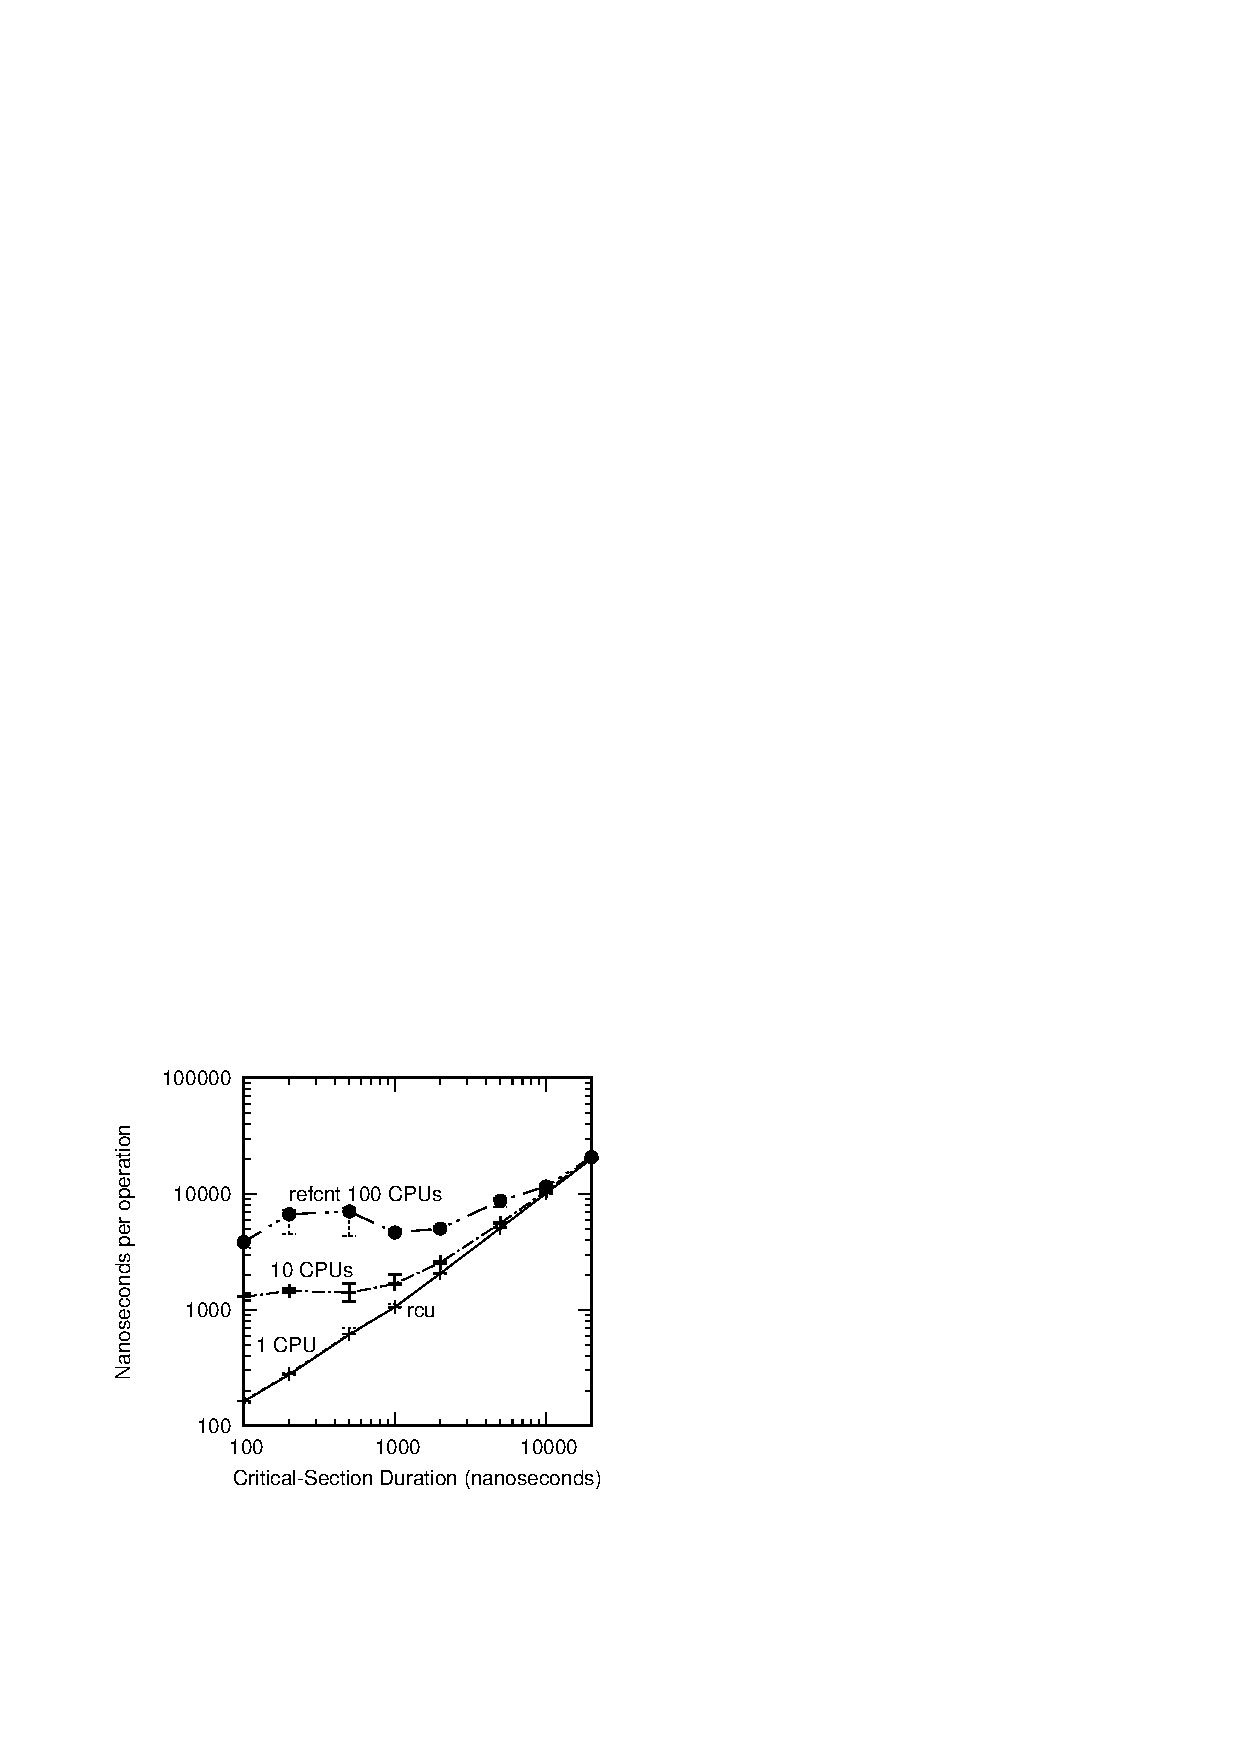
\includegraphics{defer/refRCUperfwt}}
\caption{Response Time of RCU vs. Reference Counting, 192 CPUs}
\label{fig:defer:Response Time of RCU vs. Reference Counting}
\end{figure}

하지만, reader-writer 락킹에서와 같이, RCU 의 이 성능 이득은 같은 시스템에서
Figure~\ref{fig:defer:Response Time of RCU vs. Reference Counting}
에 보인 것처럼 대부분 큰 수의 CPU 와 짧은 기간의 크리티컬 섹션으로부터
나왔습니다.
더해서, reader-writer 락킹에서와 같이, 많은 시스템 콜은 (그리고 따라서 그것들이
포함하는 모든 RCU read-side 크리티컬 섹션은) 수 마이크로세컨드 내에 완료됩니다.

그러나, RCU 에 의해 발생하는 제약들은 상당히 귀찮을 수 있습니다.
예를 들어, 많은 경우, RCU read-side 크리티컬 섹션 내에서의 잠자는 것의 금지는
그 목표를 의미없게 할 수도 있습니다.
다음 섹션은 이 문제를 해결하는 동시에 적어도 일부 경우에서는 전통적 레퍼런스
카운팅의 복잡도를 줄이는 방법들을 살펴봅니다.\footnote{
	다른 경우들은 \cref{sec:defer:Hazard Pointers} 에서 설명된 해저드
	포인터 메커니즘을 통해 더 잘 처리될 수도 있습니다.}

\iffalse

However, as with reader-writer locking, the performance advantages of
RCU are most pronounced for short-duration critical sections and for
large numbers of CPUs, as shown in
Figure~\ref{fig:defer:Response Time of RCU vs. Reference Counting}
for the same system.
In addition, as with reader-writer locking, many system calls (and thus
any RCU read-side critical sections that they contain) complete in
a few microseconds.

However, the restrictions that go with RCU can be quite onerous.
For example, in many cases, the prohibition against sleeping while in an RCU
read-side critical section would defeat the entire purpose.
The next section looks at ways of addressing this problem, while also
reducing the complexity of traditional reference counting, at least in
some cases.\footnote{
	Other cases might be better served by the hazard pointers
	mechanism described in \cref{sec:defer:Hazard Pointers}.}

\fi

\subsubsection{RCU is a Bulk Reference-Counting Mechanism}
\label{sec:defer:RCU is a Bulk Reference-Counting Mechanism}

앞의 섹션에서 이야기 되었듯, 전통적 레퍼런스 카운터는 일반적으로 특정 데이터
구조, 또는 특정 데이터 구조체들의 그룹과 연관지어집니다.
하지만, 단일한 글로벌 레퍼런스 카운터를 다양한 데이터 구조를 위해 유지하는 것은
보통 이 레퍼런스 카운트를 포함하는 캐쉬 라인이 이리저리 이동되게 합니다.
그런 캐쉬 라인 움직임은 성능을 상당히 떨어뜨릴 수 있습니다.

대조적으로, RCU 의 가벼운 read-side 기능은 무시 가능한 수준의 성능 하락과 함께
극단적으로 빈번한 read-side 사용을 가능하게 하여 RCU 가 약간 또는 없는 성능
하락을 갖는 ``bulk 레퍼런스 카운팅'' 으로 사용될 수 있게 합니다.
블록되어야 하는 코드 섹션을 가로질러 단일 태스크를 통해 레퍼런스가 얻어져야만
하는 상황에서는 Sleepable RCU (SRCU)~\cite{PaulEMcKenney2006c} 가 사용될 수
있을 겁니다.
이는 레퍼런스가 한 태스크에서 다른 태스크로 ``전달되는'', 예를 들면 어떤
레퍼런스가 I/O 시작 시에 획득되고 연관된 완료 인터럽트 핸들러에서 해제되는 것과
같은 드물지는 않은 상황은 처리할 수 없을 겁니다.
(원칙적으로, 이는 SRCU 구현에 의해 처리될 수 있습니다만, 실질적으로는 이게 좋은
트레이드오프인지 아직 명확치 않습니다.)

\iffalse

As noted in the preceding section,
traditional reference counters are usually associated with a specific
data structure, or perhaps a specific group of data structures.
However, maintaining a single global reference counter for a large
variety of data structures typically results in bouncing
the cache line containing the reference count.
Such cache-line bouncing can severely degrade performance.

In contrast, RCU's lightweight read-side primitives permit
extremely frequent read-side usage with negligible performance
degradation, permitting RCU to be used as a ``bulk reference-counting''
mechanism with little or no performance penalty.
Situations where a reference must be held by a single task across a
section of code that blocks may be accommodated with
Sleepable RCU (SRCU)~\cite{PaulEMcKenney2006c}.
This fails to cover the not-uncommon situation where a reference is ``passed''
from one task to another, for example, when a reference is acquired
when starting an I/O and released in the corresponding completion
interrupt handler.
(In principle, this could be handled by the SRCU implementation,
but in practice, it is not yet clear whether this is a good tradeoff.)

\fi

물론, SRCU 는 그 자체의 제약을 가지는데, \co{srcu_read_lock()} 에서 리턴된 값이
연관된 \co{srcu_read_unlock()} 에 전달되어야 하며, 어떤 SRCU 기능도 하드웨어
인터럽트 핸들러나 non-maskable 인터럽트 (NMI) 핸들러에서 수행되어선 안된다는
것입니다.
이 제약에 의해 얼마나 많은 문제가 있는지, 그것들이 어떻게 처리되는 것이
최선인지에 대해선 아직 판단 중입니다.

\iffalse

Of course, SRCU brings restrictions of its own, namely that the
return value from \co{srcu_read_lock()} be passed into the
corresponding \co{srcu_read_unlock()}, and that no SRCU primitives
be invoked from hardware interrupt handlers or from non-maskable interrupt
(NMI) handlers.
The jury is still out as to how much of a problem is presented by
these restrictions, and as to how they can best be handled.

\fi

\subsubsection{RCU is a Poor Man's Garbage Collector}
\label{sec:defer:RCU is a Poor Man's Garbage Collector}

RCU 를 처음 배우는 사람들의 드물지 않은 느낌은 ``RCU 는 가비지 콜렉터 같은
거다!'' 입니다.
이 느낌은 상당한 사실을 담고 있지만, 잘못된 생각의 방향을 갖게 될수도 있습니다.

RCU 와 자동화된 가비지 콜레터 (GC) 사이의 관계에 대해 생각하는 최선의 방법은
RCU 는 GC 를  쓰레기를 모으는 \emph{타이밍} 을 자동으로 결정해 준다는 점에서
닮았다는 것이겠습니다만, RCU 는 GC 와 다음과 같은 점에서 다릅니다:
(1)~프로그래머는 일일이 언제 특정 데이터 구조가 정리될 수 있는지 알려야 하며,
(2)~프로그래머는 일일이 데이터가 참조되고 있을 수도 있는 RCU read-side 크리티컬
섹션을 표시해야 합니다.

이 차이점에도 불구하고, 닮은 부분도 꽤 깊습니다.
실제로, 제가 알고 있는 첫번째 RCU와 비슷한 메커니즘의 사용은 grace period 를
제어하기 위한 레퍼런스 카운트 기반 가비지 콜렉터~\cite{Kung80} 였으며, RCU 와
가비지 콜렉터 사이의 연결은 더 최근에도 이야기
되었습니다~\cite{HarshalSheth2016goRCU}.
그러나, RCU 를 생각하는 더 나은 방법이 다음 섹션에 설명되어 있습니다.

\iffalse

A not-uncommon exclamation made by people first learning about
RCU is ``RCU is sort of like a garbage collector!''
This exclamation has a large grain of truth, but it can also be
misleading.

Perhaps the best way to think of the relationship between RCU
and automatic garbage collectors (GCs) is that RCU resembles
a GC in that the \emph{timing} of collection is automatically
determined, but that RCU differs from a GC in that: (1)~the programmer
must manually indicate when a given data structure is eligible
to be collected, and (2)~the programmer must manually mark the
RCU read-side critical sections where references might be held.

Despite these differences, the resemblance does go quite deep.
In fact, the first RCU-like mechanism I am aware of used a
reference-count-based garbage collector to handle the grace
periods~\cite{Kung80}, and the connection between RCU and
garbage collection has been noted more
recently~\cite{HarshalSheth2016goRCU}.
Nevertheless, a better way of thinking of RCU is described in the
following section.

\fi

\subsubsection{RCU is an MVCC}
\label{sec:defer:RCU is an MVCC}

RCU 는 또한 단순화 된, 완화된 일관성 기준을 갖는 multi-version concurrency
contro (MVCC) 메커니즘으로 생각될 수 있습니다.
이 멀티 버전 이야기는
\cref{sec:defer:Maintain Multiple Versions of Recently Updated Objects}
에서 다루어진 바 있습니다.
하지만, 그 기본적 형태에서, RCU 는 버전 일관성을 특정 RCU 로 보호되는 데이터
원소에 대해서만 제공합니다.

그러나, 더 높은 단계에서의 버전 일관성을 복구하기 위한 여러 기법이 사용될 수
있는데, 예를 들면equence locking 을 사용하거나
(\cref{sec:together:Correlated Data Elements} 를 참고하세요)
추가적인 우회 방법을 사용하는 겁니다
(\cref{sec:together:Correlated Fields} 를 참고하세요).

\iffalse

RCU can also be thought of as a simplified multi-version concurrency
control (MVCC) mechanism with weak consistency criteria.
The multi-version aspects were touched upon in
\cref{sec:defer:Maintain Multiple Versions of Recently Updated Objects}.
However, in its native form, RCU provides version consistency only
within a given RCU-protected data element.

However, a number of techniques can be used to restore version consistency
at a higher level, for example, using sequence locking
(see \cref{sec:together:Correlated Data Elements})
or imposing additional levels of indirection
(see \cref{sec:together:Correlated Fields}).

\fi

\subsubsection{RCU Provides Existence Guarantees}
\label{sec:defer:RCU Provides Existence Guarantees}

Gamsa 등은~\cite{Gamsa99} 존재 보장에 대해 논하고 RCU 를 닮은 어떤 메커니즘이
어떻게 이런 존재 보장을 제공하기 위해 사용될 수 있는지 설명하며 (해당 PDF 의
페이지~7 의 Section~5 를 보세요),
Section~\ref{sec:locking:Lock-Based Existence Guarantees}
은 락킹을 사용해 어떻게 존재 보장을 할 수 있는지를 그렇게 하는 것의 단점과 함께
설명합니다.
그 효과는 어떤 RCU 로 보호되는 데이터 원소든 하나의 RCU read-side 크리티컬 섹션
내에서 액세스 된다면, 그 데이터 원소는 해당 RCU read-side 크리티컬 섹션의 기간
동안은 존재하는 것이 보장된다는 것입니다.

\iffalse

Gamsa et al.~\cite{Gamsa99}
discuss existence guarantees and describe how a mechanism
resembling RCU can be used to provide these existence guarantees
(see Section~5 on page~7 of the PDF), and
Section~\ref{sec:locking:Lock-Based Existence Guarantees}
discusses how to guarantee existence via locking, along with the
ensuing disadvantages of doing so.
The effect is that if any RCU-protected data element is accessed
within an RCU read-side critical section, that data element is
guaranteed to remain in existence for the duration of that RCU
read-side critical section.

\fi

\begin{listing}[tbp]
\begin{fcvlabel}[ln:defer:Existence Guarantees Enable Per-Element Locking]
\begin{VerbatimL}[commandchars=\\\@\$]
int delete(int key)
{
	struct element *p;
	int b;

	b = hashfunction(key);			\lnlbl@hash$
	rcu_read_lock();			\lnlbl@rdlock$
	p = rcu_dereference(hashtable[b]);
	if (p == NULL || p->key != key) {	\lnlbl@chkkey$
		rcu_read_unlock();		\lnlbl@rdunlock1$
		return 0;			\lnlbl@ret_0:a$
	}
	spin_lock(&p->lock);			\lnlbl@acq$
	if (hashtable[b] == p && p->key == key) {\lnlbl@chkkey2$
		rcu_read_unlock();		\lnlbl@rdunlock2$
		rcu_assign_pointer(hashtable[b], NULL);\lnlbl@remove$
		spin_unlock(&p->lock);		\lnlbl@rel1$
		synchronize_rcu();		\lnlbl@sync_rcu$
		kfree(p);			\lnlbl@kfree$
		return 1;			\lnlbl@ret_1$
	}
	spin_unlock(&p->lock);			\lnlbl@rel2$
	rcu_read_unlock();			\lnlbl@rdunlock3$
	return 0;				\lnlbl@ret_0:b$
}
\end{VerbatimL}
\end{fcvlabel}
\caption{Existence Guarantees Enable Per-Element Locking}
\label{lst:defer:Existence Guarantees Enable Per-Element Locking}
\end{listing}

\begin{fcvref}[ln:defer:Existence Guarantees Enable Per-Element Locking]
Listing~\ref{lst:defer:Existence Guarantees Enable Per-Element Locking}
은 어떻게 RCU 기반의 존재 보장이 원소별 락킹을 가능하게 하는지 해쉬 테이블에서
원소 하나를 제거하는 함수를 통해 보입니다.
라인~\lnref{hash} 는 해쉬 함수를 계산하고, 라인~\lnref{rdlock} 은 RCU read-side
크리티컬 섹션에 진입합니다.
라인~\lnref{chkkey} 가 이 해쉬 테이블의 연관된 버킷이 비었거나 거기 있는 원소가
우리가 삭제하고자 하는 것이 아님을 발견하면, 라인~\lnref{rdunlock1} 은 RCU
read-side 크리티컬 섹션을 종료하고 라인~\lnref{ret_0:a} 에서 실패를 알립니다.
\end{fcvref}

\iffalse

\begin{fcvref}[ln:defer:Existence Guarantees Enable Per-Element Locking]
Listing~\ref{lst:defer:Existence Guarantees Enable Per-Element Locking}
demonstrates how RCU-based existence guarantees can enable
per-element locking via a function that deletes an element from
a hash table.
Line~\lnref{hash} computes a hash function, and line~\lnref{rdlock} enters an RCU
read-side critical section.
If line~\lnref{chkkey} finds that the corresponding bucket of the hash table is
empty or that the element present is not the one we wish to delete,
then line~\lnref{rdunlock1} exits the RCU read-side critical section and
line~\lnref{ret_0:a}
indicates failure.
\end{fcvref}

\fi

\QuickQuiz{
	우리가 제거하려는 원소가
	Listing~\ref{lst:defer:Existence Guarantees Enable Per-Element Locking} 의
        라인~\ref{ln:defer:Existence Guarantees Enable Per-Element Locking:chkkey}
	의 리스트의 첫번째 원소가 아니면 어떻게 되죠?

	\iffalse

	What if the element we need to delete is not the first element
	of the list on
        line~\ref{ln:defer:Existence Guarantees Enable Per-Element Locking:chkkey} of
	Listing~\ref{lst:defer:Existence Guarantees Enable Per-Element Locking}?

	\fi

}\QuickQuizAnswer{
	Listing~\ref{lst:locking:Per-Element Locking Without Existence Guarantees}
	에서와 같이, 이것은 체이닝이 없는 매우 간단한 해쉬 테이블이며, 따라서
	특정 버킷의 유일한 원소는 첫번째 원소입니다.
	독자 여러분은 다시 한번 이 예를 완전한 체이닝을 갖는 해쉬 테이블로
	조정해 보실 수 있겠습니다.
	그럴 기력이 없는 독자 분들은
	\cref{chp:Data Structures} 를 참고하고 싶으실 수도 있겠네요.

	\iffalse

	As with
	Listing~\ref{lst:locking:Per-Element Locking Without Existence Guarantees},
	this is a very simple hash table with no chaining, so the only
	element in a given bucket is the first element.
	The reader is again invited to adapt this example to a hash table with
	full chaining.
	Less energetic reader might wish to refer to
	\cref{chp:Data Structures}.

	\fi

}\QuickQuizEnd

\begin{fcvref}[ln:defer:Existence Guarantees Enable Per-Element Locking]
그렇지 않다면, 라인~\lnref{acq} 는 update-side 스핀락을 획득하고,
라인~\lnref{chkkey2} 는 이어서 이 원소가 여전히 우리가 원하는 것인지
검사합니다.
만약 그렇다면, 라인~\lnref{rdunlock2} 는 이 RCU read-side 크리티컬 섹션을
나오고, 라인~\lnref{remove} 는 이것을 테이블에서 삭제하며, 라인~\lnref{rel1}
에서 락을 해제하고, 라인~\lnref{sync_rcu} 에서 앞서서부터 존재해온 모든 RCU
read-side 크리티컬 섹션이 완료되길 기다리며, 라인~\lnref{kfree} 에서 이번에
제거된 원소를 메모리 해제하고, 라인~\lnref{ret_1} 에서 성공을 알립니다.
만약 이 원소가 더이상 우리가 원하던 것이 아니었다면, 라인~\lnref{rel2} 에서 이
락을 내려놓고, 라인~\lnref{rdunlock3} 에서 RCU read-side 크리티컬 섹션을 나온
후, 라인~\lnref{ret_0:b} 에서 이 특정 키를 제거하는데 실패했음을 알립니다.
\end{fcvref}

\iffalse

\begin{fcvref}[ln:defer:Existence Guarantees Enable Per-Element Locking]
Otherwise, line~\lnref{acq} acquires the update-side spinlock, and
line~\lnref{chkkey2} then checks that the element is still the one that we want.
If so, line~\lnref{rdunlock2} leaves the RCU read-side critical section,
line~\lnref{remove} removes it from the table, line~\lnref{rel1} releases
the lock, line~\lnref{sync_rcu} waits for all pre-existing RCU read-side critical
sections to complete, line~\lnref{kfree} frees the newly removed element,
and line~\lnref{ret_1} indicates success.
If the element is no longer the one we want, line~\lnref{rel2} releases
the lock, line~\lnref{rdunlock3} leaves the RCU read-side critical section,
and line~\lnref{ret_0:b} indicates failure to delete the specified key.
\end{fcvref}

\fi

\QuickQuizSeries{%
\QuickQuizB{
	\begin{fcvref}[ln:defer:Existence Guarantees Enable Per-Element Locking]
	Listing~\ref{lst:defer:Existence Guarantees Enable Per-Element Locking}
	의 라인~\lnref{rdunlock2} 에서는 라인\lnref{rel1} 에서 락을 내려놓기
	전에 RCU read-side 크리티컬 섹션을 빠져나가는게 왜 괜찮나요?
	\end{fcvref}

	\iffalse

	\begin{fcvref}[ln:defer:Existence Guarantees Enable Per-Element Locking]
	Why is it OK to exit the RCU read-side critical section on
	line~\lnref{rdunlock2} of
	Listing~\ref{lst:defer:Existence Guarantees Enable Per-Element Locking}
	before releasing the lock on line~\lnref{rel1}?
	\end{fcvref}

	\fi

}\QuickQuizAnswerB{
	\begin{fcvref}[ln:defer:Existence Guarantees Enable Per-Element Locking]
	첫째로, 라인~\lnref{chkkey2} 에서의 두번째 검사는 어떤 다른 CPU 가 이
	원소를 우리가 락을 획득하려 기다리는 사이에 제거했을지도 모르므로
	필요함을 알아 두시기 바랍니다.
	그러나, 우리가 이 락을 획득하는 사이 RCU read-side 크리티컬 섹션 내에
	있었다는 사실은 이 원소가 재할당되고 이 해쉬 테이블에 재삽입되었을
	가능성이 없음을 보장합니다.
	더 나아가, 일단 우리가 이 락을 획득했다면, 그 락 자체가 이 원소의
	존재를 보장하므로, 우린 더이상 이 RCU read-side 크리티컬 섹션 내에 있을
	필요가 없습니다.

	이 원소의 키를 재검사 할 필요가 있는가 하는 질문은 독자 여러분의
	연습문제로 남겨둡니다.
	\end{fcvref}

	\iffalse

	\begin{fcvref}[ln:defer:Existence Guarantees Enable Per-Element Locking]
	First, please note that the second check on line~\lnref{chkkey2} is
	necessary because some other
	CPU might have removed this element while we were waiting
	to acquire the lock.
	However, the fact that we were in an RCU read-side critical section
	while acquiring the lock guarantees that this element could not
	possibly have been re-allocated and re-inserted into this
	hash table.
	Furthermore, once we acquire the lock, the lock itself guarantees
	the element's existence, so we no longer need to be in an
	RCU read-side critical section.

	The question as to whether it is necessary to re-check the
	element's key is left as an exercise to the reader.
	% A re-check is necessary if the key can mutate or if it is
	% necessary to reject deleted entries (in cases where deletion
	% is recorded by mutating the key.
	\end{fcvref}

	\fi

}\QuickQuizEndB
%
\QuickQuizE{
	\begin{fcvref}[ln:defer:Existence Guarantees Enable Per-Element Locking]
	Listing~\ref{lst:defer:Existence Guarantees Enable Per-Element Locking}
	의 라인~\lnref{rdunlock3} 에서는 왜 라인~\lnref{rel2} 에서 락을
	내려놓기 전에 RCU read-side 크리티컬 섹션을 빠져나가지 않나요?
	\end{fcvref}

	\iffalse

	\begin{fcvref}[ln:defer:Existence Guarantees Enable Per-Element Locking]
	Why not exit the RCU read-side critical section on
	line~\lnref{rdunlock3} of
	Listing~\ref{lst:defer:Existence Guarantees Enable Per-Element Locking}
	before releasing the lock on line~\lnref{rel2}?
	\end{fcvref}

	\fi

}\QuickQuizAnswerE{
	우리가 이 두 라인의 순서를 바꾼다고 생각해 봅시다.
	그러면 이 코드는 다음 순서의 이벤트에 취약해 집니다:

	\iffalse

	Suppose we reverse the order of these two lines.
	Then this code is vulnerable to the following sequence of
	events:

	\fi

	\begin{enumerate}
	\begin{fcvref}[ln:defer:Existence Guarantees Enable Per-Element Locking]
	\item	CPU~0 가 \co{delete()} 를 호출하고, 삭제될 원소를 찾은 후,
		라인~\lnref{rdunlock2} 를 수행합니다.
		아직 원소를 삭제하지 않았지만, 곧 할겁니다.
	\item	CPU~1 이 동시에 \co{delete()} 를 호출해, 이 동일한 원소를
		제거하려 합니다.
		하지만, CPU~0 는 여전히 락을 잡고 있으므로, CPU~1 은
		라인~\lnref{acq} 에서 그걸 기다립니다.
	\item	CPU~0 이 라인~\lnref{remove} 와~\lnref{rel1} 을 수행하며,
		라인~\lnref{sync_rcu} 에서 CPU~1 이 RCU read-side 크리티컬
		섹션에서 나오길 기다립니다.
	\item	CPU~1 이 이제 이 락을 잡지만, 라인~\lnref{chkkey2} 에서의
		테스트는 CPU~0 이 이미 이 원소를 제거했으므로 실패합니다.
		CPU~1 은 이제 (이 quick quiz 를 위해 우리가
		라인~\lnref{rdunlock3} 과 교체한) 라인~\lnref{rel2} 를 수행하고
		자신의 RCU read-side 크리티컬 섹션을 빠져나갑니다.
	\item	CPU~0 은 이제 \co{synchronize_rcu()} 로부터 리턴할 수 있고,
		따라서 라인~\lnref{kfree} 를 수행해 이 원소를 freelist 로
		보냅니다.
	\item	CPU~1 이 이제 메모리 해제된, 어쩌면 이제 다른 종류의 데이터
		구조체로 이미 재할당 되었을 수도 있는 원소를 위한 락을
		내려놓으려 합니다.
		이는 심각한 메모리 오염 에러입니다.
	\end{fcvref}

	\iffalse

	\begin{fcvref}[ln:defer:Existence Guarantees Enable Per-Element Locking]
	\item	CPU~0 invokes \co{delete()}, and finds the element
		to be deleted, executing through line~\lnref{rdunlock2}.
		It has not yet actually deleted the element, but
		is about to do so.
	\item	CPU~1 concurrently invokes \co{delete()}, attempting
		to delete this same element.
		However, CPU~0 still holds the lock, so CPU~1 waits
		for it at line~\lnref{acq}.
	\item	CPU~0 executes lines~\lnref{remove} and~\lnref{rel1},
		and blocks at line~\lnref{sync_rcu} waiting for CPU~1
		to exit its RCU read-side critical section.
	\item	CPU~1 now acquires the lock, but the test on line~\lnref{chkkey2}
		fails because CPU~0 has already removed the element.
		CPU~1 now executes line~\lnref{rel2}
                (which we switched with line~\lnref{rdunlock3}
		for the purposes of this Quick Quiz)
		and exits its RCU read-side critical section.
	\item	CPU~0 can now return from \co{synchronize_rcu()},
		and thus executes line~\lnref{kfree}, sending the element to
		the freelist.
	\item	CPU~1 now attempts to release a lock for an element
		that has been freed, and, worse yet, possibly
		reallocated as some other type of data structure.
		This is a fatal memory-corruption error.
	\end{fcvref}

	\fi

	\end{enumerate}
}\QuickQuizEndE
}

독자 여러분은 이게
Section~\ref{sec:defer:RCU is a Way of Waiting for Things to Finish} 에서
설명된, 원래의 ``RCU 는 무언가가 끝나길 기다리는 방법 중 하나다'' 주제의 약간의
변종일 뿐임을 알게 될 것임을 경고 드립니다.
그것들은 또한
Section~\ref{sec:locking:Lock-Based Existence Guarantees}
에서 이야기된 락킹 기반 존재 보장 대비 데드락 내성의 장점을 알려줄 지도
모릅니다.

\iffalse

Alert readers will recognize this as only a slight variation on
the original ``RCU is a way of waiting for things to finish'' theme,
which is addressed in
Section~\ref{sec:defer:RCU is a Way of Waiting for Things to Finish}.
They might also note the deadlock-immunity advantages over the lock-based
existence guarantees discussed in
Section~\ref{sec:locking:Lock-Based Existence Guarantees}.

\fi

\subsubsection{RCU Provides Type-Safe Memory}
\label{sec:defer:RCU Provides Type-Safe Memory}

A number of lockless algorithms do not require that a given data
element keep the same identity through a given RCU read-side critical
section referencing it---but only if that data element retains the
same type.
In other words, these lockless algorithms can tolerate a given data
element being freed and reallocated as the same type of structure
while they are referencing it, but must prohibit a change in type.
This guarantee, called ``type-safe memory'' in
academic literature~\cite{Cheriton96a},
is weaker than the existence guarantees in the
previous section, and is therefore quite a bit harder to work with.
Type-safe memory algorithms in the Linux kernel make use of slab caches,
specially marking these caches with \co{SLAB_TYPESAFE_BY_RCU}
so that RCU is used when returning a freed-up
slab to system memory.
This use of RCU guarantees that any in-use element of
such a slab will remain in that slab, thus retaining its type,
for the duration of any pre-existing RCU read-side critical sections.

\QuickQuiz{
	But what if there is an arbitrarily long series of RCU
	read-side critical sections in multiple threads, so that at
	any point in time there is at least one thread in the system
	executing in an RCU read-side critical section?
	Wouldn't that prevent any data from a \co{SLAB_TYPESAFE_BY_RCU}
	slab ever being returned to the system, possibly resulting
	in OOM events?
}\QuickQuizAnswer{
	There could certainly be an arbitrarily long period of time
	during which at least one thread is always in an RCU read-side
	critical section.
	However, the key words in the description in
	Section~\ref{sec:defer:RCU Provides Type-Safe Memory}
	are ``in-use'' and ``pre-existing''.
	Keep in mind that a given RCU read-side critical section is
	conceptually only permitted to gain references to data elements
	that were in use at the beginning of that critical section.
	Furthermore, remember that a slab cannot be returned to the
	system until all of its data elements have been freed, in fact,
	the RCU grace period cannot start until after they have all been
	freed.

	Therefore, the slab cache need only wait for those RCU read-side
	critical sections that started before the freeing of the last element
	of the slab.
	This in turn means that any RCU grace period that begins after
	the freeing of the last element will do---the slab may be returned
	to the system after that grace period ends.
}\QuickQuizEnd

It is important to note that \co{SLAB_TYPESAFE_BY_RCU} will
\emph{in no way}
prevent \co{kmem_cache_alloc()} from immediately reallocating
memory that was just now freed via \co{kmem_cache_free()}!
In fact, the \co{SLAB_TYPESAFE_BY_RCU}-protected data structure
just returned by \co{rcu_dereference()} might be freed and reallocated
an arbitrarily large number of times, even when under the protection
of \co{rcu_read_lock()}.
Instead, \co{SLAB_TYPESAFE_BY_RCU} operates by preventing
\co{kmem_cache_free()}
from returning a completely freed-up slab of data structures
to the system until after an RCU grace period elapses.
In short, although a given RCU read-side critical section might see a
given \co{SLAB_TYPESAFE_BY_RCU} data element being freed and reallocated
arbitrarily often, the element's type is guaranteed not to change until
that critical section has completed.

These algorithms therefore typically use a validation step that checks
to make sure that the newly referenced data structure really is the one
that was requested~\cite[Section~2.5]{LaninShasha1986TSM}.
These validation checks require that portions of the data structure
remain untouched by the free-reallocate process.
Such validation checks are usually very hard to get right, and can
hide subtle and difficult bugs.

Therefore, although type-safety-based lockless algorithms can be extremely
helpful in a very few difficult situations, you should instead use existence
guarantees where possible.
Simpler is after all almost always better!

\subsubsection{RCU is a Way of Waiting for Things to Finish}
\label{sec:defer:RCU is a Way of Waiting for Things to Finish}

As noted in Section~\ref{sec:defer:RCU Fundamentals}
an important component
of RCU is a way of waiting for RCU readers to finish.
One of
RCU's great strength is that it allows you to wait for each of
thousands of different things to finish without having to explicitly
track each and every one of them, and without having to worry about
the performance degradation, scalability limitations, complex deadlock
scenarios, and memory-leak hazards that are inherent in schemes that
use explicit tracking.

In this section, we will show how \co{synchronize_sched()}'s
read-side counterparts (which include anything that disables preemption,
along with hardware operations and
primitives that disable interrupts) permit you to implement interactions with
non-maskable interrupt
(NMI) handlers that would be quite difficult if using locking.
This approach has been called ``Pure RCU''~\cite{PaulEdwardMcKenneyPhD},
and it is used in a number of places in the Linux kernel.

The basic form of such ``Pure RCU'' designs is as follows:

\begin{enumerate}
\item	Make a change, for example, to the way that the OS reacts to an NMI\@.
\item	Wait for all pre-existing read-side critical sections to
	completely finish (for example, by using the
	\co{synchronize_sched()} primitive).
	The key observation here is that subsequent RCU read-side critical
	sections are guaranteed to see whatever change was made.
\item	Clean up, for example, return status indicating that the
	change was successfully made.
\end{enumerate}

The remainder of this section presents example code adapted from
the Linux kernel.
In this example, the \co{timer_stop} function uses
\co{synchronize_sched()} to ensure that all in-flight NMI
notifications have completed before freeing the associated resources.
A simplified version of this code is shown
Listing~\ref{lst:defer:Using RCU to Wait for NMIs to Finish}.

\begin{listing}[tbp]
\begin{fcvlabel}[ln:defer:Using RCU to Wait for NMIs to Finish]
\begin{VerbatimL}[commandchars=\\\@\$]
struct profile_buffer {				\lnlbl@struct:b$
	long size;
	atomic_t entry[0];
};						\lnlbl@struct:e$
static struct profile_buffer *buf = NULL;	\lnlbl@struct:buf$

void nmi_profile(unsigned long pcvalue)		\lnlbl@nmi_profile:b$
{
	struct profile_buffer *p = rcu_dereference(buf);\lnlbl@nmi_profile:rcu_deref$

	if (p == NULL)				\lnlbl@nmi_profile:if_NULL$
		return;				\lnlbl@nmi_profile:ret:a$
	if (pcvalue >= p->size)			\lnlbl@nmi_profile:if_oor$
		return;				\lnlbl@nmi_profile:ret:b$
	atomic_inc(&p->entry[pcvalue]);		\lnlbl@nmi_profile:inc$
}						\lnlbl@nmi_profile:e$

void nmi_stop(void)				\lnlbl@nmi_stop:b$
{
	struct profile_buffer *p = buf;		\lnlbl@nmi_stop:fetch$

	if (p == NULL)				\lnlbl@nmi_stop:if_NULL$
		return;				\lnlbl@nmi_stop:ret$
	rcu_assign_pointer(buf, NULL);		\lnlbl@nmi_stop:NULL$
	synchronize_sched();			\lnlbl@nmi_stop:sync_sched$
	kfree(p);				\lnlbl@nmi_stop:kfree$
}						\lnlbl@nmi_stop:e$
\end{VerbatimL}
\end{fcvlabel}
\caption{Using RCU to Wait for NMIs to Finish}
\label{lst:defer:Using RCU to Wait for NMIs to Finish}
\end{listing}

\begin{fcvref}[ln:defer:Using RCU to Wait for NMIs to Finish:struct]
\Clnrefrange{b}{e} define a \co{profile_buffer} structure, containing a
size and an indefinite array of entries.
Line~\lnref{buf} defines a pointer to a profile buffer, which is
presumably initialized elsewhere to point to a dynamically allocated
region of memory.
\end{fcvref}

\begin{fcvref}[ln:defer:Using RCU to Wait for NMIs to Finish:nmi_profile]
\Clnrefrange{b}{e} define the \co{nmi_profile()} function,
which is called from within an NMI handler.
As such, it cannot be preempted, nor can it be interrupted by a normal
interrupts handler, however, it is still subject to delays due to cache misses,
ECC errors, and cycle stealing by other hardware threads within the same
core.
Line~\lnref{rcu_deref} gets a local pointer to the profile buffer using the
\co{rcu_dereference()} primitive to ensure memory ordering on
DEC Alpha, and
lines~\lnref{if_NULL} and~\lnref{ret:a} exit from this function if there is no
profile buffer currently allocated, while lines~\lnref{if_oor} and~\lnref{ret:b}
exit from this function if the \co{pcvalue} argument
is out of range.
Otherwise, line~\lnref{inc} increments the profile-buffer entry indexed
by the \co{pcvalue} argument.
Note that storing the size with the buffer guarantees that the
range check matches the buffer, even if a large buffer is suddenly
replaced by a smaller one.
\end{fcvref}

\begin{fcvref}[ln:defer:Using RCU to Wait for NMIs to Finish:nmi_stop]
\Clnrefrange{b}{e} define the \co{nmi_stop()} function,
where the caller is responsible for mutual exclusion (for example,
holding the correct lock).
Line~\lnref{fetch} fetches a pointer to the profile buffer, and
lines~\lnref{if_NULL} and~\lnref{ret} exit the function if there is no buffer.
Otherwise, line~\lnref{NULL} \co{NULL}s out the profile-buffer pointer
(using the \co{rcu_assign_pointer()} primitive to maintain
memory ordering on weakly ordered machines),
and line~\lnref{sync_sched} waits for an RCU Sched grace period to elapse,
in particular, waiting for all non-preemptible regions of code,
including NMI handlers, to complete.
Once execution continues at line~\lnref{kfree}, we are guaranteed that
any instance of \co{nmi_profile()} that obtained a
pointer to the old buffer has returned.
It is therefore safe to free the buffer, in this case using the
\co{kfree()} primitive.
\end{fcvref}

\QuickQuiz{
	Suppose that the \co{nmi_profile()} function was preemptible.
	What would need to change to make this example work correctly?
}\QuickQuizAnswer{
	One approach would be to use
	\co{rcu_read_lock()} and \co{rcu_read_unlock()}
	in \co{nmi_profile()}, and to replace the
	\co{synchronize_sched()} with \co{synchronize_rcu()},
	perhaps as shown in
	Listing~\ref{lst:defer:Using RCU to Wait for Mythical Preemptible NMIs to Finish}.
%
\begin{listing}[tb]
\begin{VerbatimL}
struct profile_buffer {
	long size;
	atomic_t entry[0];
};
static struct profile_buffer *buf = NULL;

void nmi_profile(unsigned long pcvalue)
{
	struct profile_buffer *p;

	rcu_read_lock();
	p = rcu_dereference(buf);
	if (p == NULL) {
		rcu_read_unlock();
		return;
	}
	if (pcvalue >= p->size) {
		rcu_read_unlock();
		return;
	}
	atomic_inc(&p->entry[pcvalue]);
	rcu_read_unlock();
}

void nmi_stop(void)
{
	struct profile_buffer *p = buf;

	if (p == NULL)
		return;
	rcu_assign_pointer(buf, NULL);
	synchronize_rcu();
	kfree(p);
}
\end{VerbatimL}
\caption{Using RCU to Wait for Mythical Preemptible NMIs to Finish}
\label{lst:defer:Using RCU to Wait for Mythical Preemptible NMIs to Finish}
\end{listing}
%
}\QuickQuizEnd

In short, RCU makes it easy to dynamically switch among profile
buffers (you just \emph{try} doing this efficiently with atomic
operations, or at all with locking!).
However, RCU is normally used at a higher level of abstraction, as
was shown in the previous sections.

\subsubsection{RCU Usage Summary}
\label{sec:defer:RCU Usage Summary}

At its core, RCU is nothing more nor less than an API that provides:

\begin{enumerate}
\item	a publish-subscribe mechanism for adding new data,
\item	a way of waiting for pre-existing RCU readers to finish, and
\item	a discipline of maintaining multiple versions to permit change
	without harming or unduly delaying concurrent RCU readers.
\end{enumerate}

That said, it is possible to build higher-level constructs
on top of RCU, including the reader-writer-locking, reference-counting,
and existence-guarantee constructs listed in the earlier sections.
Furthermore, I have no doubt that the Linux community will continue to
find interesting new uses for RCU,
as well as for any of a number of other synchronization primitives.

\begin{figure}[tbh]
\centering
\resizebox{3in}{!}{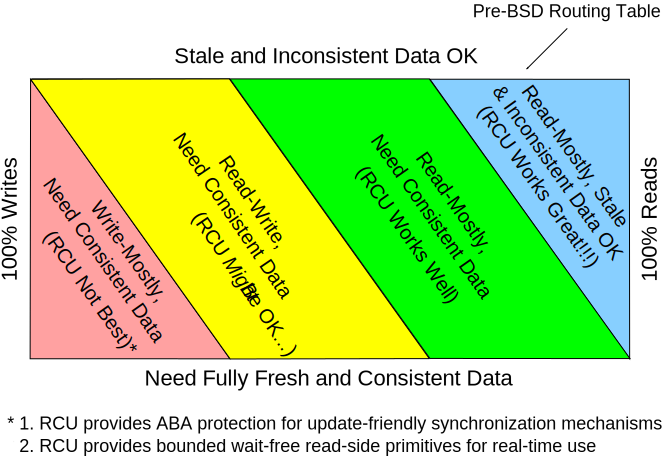
\includegraphics{defer/RCUApplicability}}
\caption{RCU Areas of Applicability}
\label{fig:defer:RCU Areas of Applicability}
\end{figure}

In the meantime,
Figure~\ref{fig:defer:RCU Areas of Applicability}
shows some rough rules of thumb on where RCU is most helpful.

As shown in the blue box at the top of the figure, RCU works best if
you have read-mostly data where stale and inconsistent
data is permissible (but see below for more information on stale and
inconsistent data).
The canonical example of this case in the Linux kernel is routing tables.
Because it may have taken many seconds or even minutes for the
routing updates to propagate across the Internet, the system
has been sending packets the wrong way for quite some time.
Having some small probability of continuing to send some of them the wrong
way for a few more milliseconds is almost never a problem.

If you have a read-mostly workload where consistent data is required,
RCU works well, as shown by the green ``read-mostly, need consistent data''
box.
One example of this case is the Linux kernel's mapping from user-level
System-V semaphore IDs to the corresponding in-kernel data structures.
Semaphores tend to be used far more frequently than they are created
and destroyed, so this mapping is read-mostly.
However, it would be erroneous to perform a semaphore operation on
a semaphore that has already been deleted.
This need for consistency is handled by using the lock in the
in-kernel semaphore data structure, along with a ``deleted''
flag that is set when deleting a semaphore.
If a user ID maps to an in-kernel data structure with the
``deleted'' flag set, the data structure is ignored, so that
the user ID is flagged as invalid.

Although this requires that the readers acquire a lock for the
data structure representing the semaphore itself,
it allows them to dispense with locking for the
mapping data structure.
The readers therefore locklessly
traverse the tree used to map from ID to data structure,
which in turn greatly improves performance, scalability, and
real-time response.

As indicated by the yellow ``read-write'' box, RCU can also be useful
for read-write
workloads where consistent data is required, although usually in
conjunction with a number of other synchronization primitives.
For example, the directory-entry cache in recent Linux kernels uses RCU in
conjunction with sequence locks, per-CPU locks, and per-data-structure
locks to allow lockless traversal of pathnames in the common case.
Although RCU can be very beneficial in this read-write case, such
use is often more complex than that of the read-mostly cases.

Finally, as indicated by the red box at the bottom of the figure,
update-mostly workloads requiring
consistent data are rarely good places to use RCU, though there are some
exceptions~\cite{MathieuDesnoyers2012URCU}.
In addition, as noted in
Section~\ref{sec:defer:RCU Provides Type-Safe Memory},
within the Linux kernel, the \co{SLAB_TYPESAFE_BY_RCU}
slab-allocator flag provides type-safe memory to RCU readers, which can
greatly simplify non-blocking synchronization and other lockless
algorithms.

In short, RCU is an API that includes a publish-subscribe mechanism for
adding new data, a way of waiting for pre-existing RCU readers to finish,
and a discipline of maintaining multiple versions to allow updates to
avoid harming or unduly delaying concurrent RCU readers.
This RCU API is best suited for read-mostly situations, especially if
stale and inconsistent data can be tolerated by the application.

% defer/rcuAPI.tex

\subsection{RCU Linux-Kernel API}
\label{sec:defer:RCU Linux-Kernel API}
\OriginallyPublished{Section}{sec:defer:RCU Linux-Kernel API}{RCU Linux-Kernel API}{Linux Weekly News}{PaulEMcKenney2008WhatIsRCUAPI}

이 섹션은 RCU를 그것의 리눅스 커널 API의 관점에서 바라봅니다.
Section~\ref{sec:defer:RCU has a Family of Wait-to-Finish APIs}
은 RCU 의 wait-to-finish API들을, 그리고
Section~\ref{sec:defer:RCU has Publish-Subscribe and Version-Maintenance APIs}
에서는 RCU 의 publish-subscribe 와 version-maintenance API 들을 소개합니다.
마지막으로,
Section~\ref{sec:defer:So, What is RCU Really?}
에서는 결론을 정리합니다.
\iffalse

This section looks at RCU from the viewpoint of its Linux-kernel API.
Section~\ref{sec:defer:RCU has a Family of Wait-to-Finish APIs}
presents RCU's wait-to-finish APIs, and
Section~\ref{sec:defer:RCU has Publish-Subscribe and Version-Maintenance APIs}
presents RCU's publish-subscribe and version-maintenance APIs.
Finally,
Section~\ref{sec:defer:So, What is RCU Really?}
presents concluding remarks.
\fi

\subsubsection{RCU has a Family of Wait-to-Finish APIs}
\label{sec:defer:RCU has a Family of Wait-to-Finish APIs}

\begin{sidewaystable*}[htbp]
\centering
\scriptsize\tymin=1.4in
\begin{tabulary}{7.8in}{L|L|L|L|L|L}
Attribute &
    RCU Classic &
	RCU BH &
	    RCU Sched &
		Realtime RCU &
		    SRCU \\
\hline
\hline
Purpose &
    Original &
	Prevent DDoS attacks &
	    Wait for preempt-disable regions, hardirqs, \& NMIs &
	        Realtime response &
		    Sleeping readers \\
\hline
Availability &
    2.5.43 &
	2.6.9 &
	    2.6.12 &
		2.6.26 &
		    2.6.19 \\
\hline
Read-side primitives &
    \begin{minipage}[t]{1.4in}{ \raggedright
      \co{rcu_read_lock()}~! \\
      \co{rcu_read_unlock()}~! }\end{minipage} &
	\begin{minipage}[t]{1.4in}{ \raggedright
	  \co{rcu_read_lock_bh()} \\
	  \co{rcu_read_unlock_bh()} }\end{minipage} &
	    \begin{minipage}[t]{1.4in}{ \raggedright
	      \co{preempt_disable()} \\
	      \co{preempt_enable()} \\
	      (and friends) }\end{minipage} &
	        \begin{minipage}[t]{1.4in}{ \raggedright
		  \co{rcu_read_lock()} \\
		  \co{rcu_read_unlock()} }\end{minipage} &
		    \begin{minipage}[t]{1.4in}{ \raggedright
		      \co{srcu_read_lock()} \\
		      \co{srcu_read_unlock()} }\end{minipage} \\
\hline
{ Update-side primitives (synchronous) } &
    { \co{synchronize_rcu()} \co{synchronize_net()} } &
	\co{synchronize_rcu_bh()} &
	    \co{synchronize_sched()} &
	        { \co{synchronize_rcu()} \co{synchronize_net()} } &
		    \co{synchronize_srcu()} \\
\hline
{ Update-side primitives (asynchronous/callback) } &
    \co{call_rcu()} ! &
	\co{call_rcu_bh()} &
	    \co{call_rcu_sched()} &
	        \co{call_rcu()} &
		    \co{call_srcu()} \\
\hline
{ Update-side primitives (wait for callbacks) } &
    \co{rcu_barrier()} &
	\co{rcu_barrier_bh()} &
	    \co{rcu_barrier_sched()} &
	        \co{rcu_barrier()} &
		    N/A \\
\hline
Type-safe memory &
    \co{SLAB_DESTROY_BY_RCU} &
	&
	    &
	        \co{SLAB_DESTROY_BY_RCU} &
		    \\
\hline
Read side constraints &
    No blocking &
	No bottom-half (BH) enabling &
	    No blocking &
	        Only preemption and lock acquisition &
		    No \co{synchronize_srcu()} wtih same \co{srcu_struct} \\
\hline
Read side overhead &
    Preempt disable/enable (free on non-PREEMPT) &
	BH disable/enable &
	    Preempt disable/enable (free on non-PREEMPT) &
	        Simple instructions, irq disable/enable &
		    Simple instructions, preempt disable/enable, memory barriers \\
\hline
Asynchronous update-side overhead &
    sub-microsecond &
	sub-microsecond &
	    sub-microsecond &
	        sub-microsecond &
		    N/A \\
\hline
Grace-period latency &
    10s of milliseconds &
	10s of milliseconds &
	    10s of milliseconds &
	        10s of milliseconds &
		    10s of milliseconds \\
\hline
Non-\co{PREEMPT_RT} implementation &
    RCU Classic &
	RCU BH &
	    RCU Classic &
	        Preemptible RCU &
		    SRCU \\
\hline
\co{PREEMPT_RT} implementation &
    Preemptible RCU &
	Realtime RCU &
	    Forced Schedule on all CPUs &
	        Realtime RCU &
		    SRCU \\
\end{tabulary}
\caption{RCU Wait-to-Finish APIs}
\label{tab:defer:RCU Wait-to-Finish APIs}
\end{sidewaystable*}

``RCU 는 무엇인가'' 에 대한 가장 직접적인 답변은 RCU 는 리눅스 커널에서
사용되는 API 라는 것으로, 각각 잠들 수 없는 버전과 잠들 수 있는 버전 API 들의
RCU 읽기 쓰레드 기다리기 부분을 보이는
Table~\ref{tab:defer:RCU Wait-to-Finish APIs},
그리고 그 API 의 publish-subscribe 부분을 보이는
Table~\ref{tab:defer:RCU Publish-Subscribe and Version Maintenance APIs} 에
요약되어 있습니다.
\iffalse

The most straightforward answer to ``what is RCU'' is that RCU is
an API used in the Linux kernel, as summarized by
Table~\ref{tab:defer:RCU Wait-to-Finish APIs},
which shows the wait-for-RCU-readers portions of the non-sleepable and
sleepable APIs, respectively,
and by
Table~\ref{tab:defer:RCU Publish-Subscribe and Version Maintenance APIs},
which shows the publish-subscribe portions of the API.
\fi

RCU 가 처음이라면
Table~\ref{tab:defer:RCU Wait-to-Finish APIs} 의 행들 중 하나에만 집중해 볼
것을 고려해 볼만 한데, 각각의 행은 리눅스 커널의 RCU API 패밀리 중 하나의
멤버를 요약하고 있습니다.
예를 들어, 리눅스 커널에서 RCU 가 어떻게 사용되는지를 이해하고자 하는게 주된
목표라면, ``RCU Classic'' 가장 자주 사용되므로 여기서부터 시작하는게 좋을
것입니다.
반면에, 자신의 이익을 위해 RCU 를 이해하고자 한다면 ``SRCU'' 가 가장 간단한 API
를 제공합니다.
나중에도 언제든 다른 행을 볼 수 있습니다.

이미 RCU 에 친숙하다면, 이 표들은 유용한 레퍼런스로 사용될 수 있을 겁니다.
\iffalse

If you are new to RCU, you might consider focusing on just one
of the columns in
Table~\ref{tab:defer:RCU Wait-to-Finish APIs},
each of which summarizes one member of the Linux kernel's RCU API family.
For example, if you are primarily interested in understanding how RCU
is used in the Linux kernel, ``RCU Classic'' would be the place to start,
as it is used most frequently.
On the other hand, if you want to understand RCU for its own sake,
``SRCU'' has the simplest API.
You can always come back for the other columns later.

If you are already familiar with RCU, these tables can
serve as a useful reference.
\fi

\QuickQuiz{}
	Table~\ref{tab:defer:RCU Wait-to-Finish APIs} 의 일부 셀들은 왜 느낌표
	(``!'') 를 가지고 있나요?
	\iffalse

	Why do some of the cells in
	Table~\ref{tab:defer:RCU Wait-to-Finish APIs}
	have exclamation marks (``!'')?
	\fi
\QuickQuizAnswer{
	느낌표와 함께 표시된 API 멤버들 (\co{rcu_read_lock()},
	\co{rcu_read_unlock()}, 그리고 \co{call_rcu()}) 만이 과거 90년대 중반에
	Paul E. McKenney 가 신경썼던 리눅스 RCU API 의 멤버들입니다.
	이 시절에는, 그는 그가 RCU 에 대해 알아야 할 것들을 모두 알고 있다는
	잘못된 인상을 가지고 있었습니다.
	\iffalse

	The API members with exclamation marks (\co{rcu_read_lock()},
	\co{rcu_read_unlock()}, and \co{call_rcu()}) were the
	only members of the Linux RCU API that Paul E. McKenney was aware
	of back in the mid-90s.
	During this timeframe, he was under the mistaken impression that
	he knew all that there is to know about RCU.
	\fi
} \QuickQuizEnd

이 ``RCU Classic'' 행은 RCU read-side 크리티컬 섹션들은 \co{rcu_read_lock()} 과
\co{rcu_read_unlock()} 으로 구분지어지고 중첩될수도 있는, 최초의 RCU 구현에
해당합니다.
여기에 연관되는 동기적인 업데이트 쪽 기능들인 \co{synchronize_rcu()} 와 그것과
같은 의미인 \co{synchronize_net()} 은 동시에 실행중인 RCU read-side 크리티컬
섹션들이 모두 완료되기를 기다립니다.
이 기다림의 길이는 ``grace period'' 라고 알려져 있습니다.
비동기적인 업데이트 쪽 기능인 \co{call_rcu()} 는 뒤따르는 grace period 후에
특정 함수를 특정 인자와 함께 호출해 줍니다.
예를 들어, \co{call_rcu(p,f);} 는 다음의 grace period 후에 ``RCU callback''
\co{f(p)} 의 호출이 이뤄지게 합니다.
\co{call_rcu()} 를 사용하는 리눅스 커널 모듈을 언로딩 한다던가 해서 모든 RCU
callback 들이 완료되기를 기다려야만 하는 상황도
존재합니다~\cite{PaulEMcKenney2007rcubarrier}.
\co{rcu_barrier()} 기능이 그 일을 합니다.
더 최신의 계층적 RCU~\cite{PaulEMcKenney2008HierarchicalRCU} 구현 또한 ``RCU
Classic'' 시맨틱을 고수함을 알아두세요.
\iffalse

The ``RCU Classic'' column corresponds to the original RCU implementation,
in which RCU read-side critical sections are delimited by
\co{rcu_read_lock()} and \co{rcu_read_unlock()}, which
may be nested.
The corresponding synchronous update-side primitives,
\co{synchronize_rcu()}, along with its synonym
\co{synchronize_net()}, wait for any currently executing
RCU read-side critical sections to complete.
The length of this wait is known as a ``grace period''.
The asynchronous update-side primitive, \co{call_rcu()},
invokes a specified function with a specified argument after a
subsequent grace period.
For example, \co{call_rcu(p,f);} will result in
the ``RCU callback'' \co{f(p)}
being invoked after a subsequent grace period.
There are situations,
such as when unloading a Linux-kernel module that uses \co{call_rcu()},
when it is necessary to wait for all
outstanding RCU callbacks to complete~\cite{PaulEMcKenney2007rcubarrier}.
The \co{rcu_barrier()} primitive does this job.
Note that the more recent hierarchical
RCU~\cite{PaulEMcKenney2008HierarchicalRCU}
implementation also adheres to ``RCU Classic'' semantics.
\fi

마지막으로, RCU 는
Section~\ref{sec:defer:RCU is a Way of Providing Type-Safe Memory} 에서 설명한
것처럼 type-safe 메모리~\cite{Cheriton96a} 를 제공하는데 사용될 수도 있습니다.
RCU 의 문맥에서, type-safe 메모리는 주어진 데이터 원소가 그것에 접근하는 모든
RCU read-side 크리티컬 섹션 사이에서 그 타입이 바뀌지 않는다는 것을 보장합니다.
RCU 기반의 type-safe 메모리를 사용하기 위해서는 \co{SLAB_DESTROY_BY_RCU} 를
\co{kmem_cache_create()} 에 넘겨야 합니다.
\co{SLAB_DESTROY_BY_RCU} 는 \co{kmem_cache_alloc()} 이 \co{kmem_cache_free()}
로 자유가 된 메모리를 즉시 재할당 하는 것을 막는 일은 \emph{결코} 하지 않음을
알아두는 게 중요합니다!
사실, \co{rcu_dereference} 로 리턴된, \co{SLAB_DESTROY_RCU} 로 보호되는 데이터
구조체는 상당히 여러번 메모리 해제되고 재할당 될 수 있는데, 심지어
\co{rcu_read_lock()} 으로 보호되고 있을 때도 그러합니다.
대신, \co{SLAB_DESTROY_BY_RCU} 는 RCU grace period 가 끝나기 전까지는
\co{kmem_cache_free()} 가 완전히 해제된 데이터 구조체들의 slab 을 시스템에
반납하는 것을 방지해 줍니다.
짧게 말해서, 비록 데이터 원소가 굉장히 자주 해제되고 재할당될 수 있지만, 최소한
그것의 타입은 똑같이 남아있을 겁니다.
\iffalse

Finally, RCU may be used to provide
type-safe memory~\cite{Cheriton96a}, as described in
Section~\ref{sec:defer:RCU is a Way of Providing Type-Safe Memory}.
In the context of RCU, type-safe memory guarantees that a given
data element will not change type during any RCU read-side critical section
that accesses it.
To make use of RCU-based type-safe memory, pass
\co{SLAB_DESTROY_BY_RCU} to
\co{kmem_cache_create()}.
It is important to note that \co{SLAB_DESTROY_BY_RCU} will
\emph{in no way}
prevent \co{kmem_cache_alloc()} from immediately reallocating
memory that was just now freed via \co{kmem_cache_free()}!
In fact, the \co{SLAB_DESTROY_BY_RCU}-protected data structure
just returned by \co{rcu_dereference} might be freed and reallocated
an arbitrarily large number of times, even when under the protection
of \co{rcu_read_lock()}.
Instead, \co{SLAB_DESTROY_BY_RCU} operates by preventing
\co{kmem_cache_free()}
from returning a completely freed-up slab of data structures
to the system until after an RCU grace period elapses.
In short, although the data element might be freed and reallocated arbitrarily
often, at least its type will remain the same.
\fi

\QuickQuiz{}
	많은 수의 RCU read-side 크리티컬 섹션들이 \co{synchronize_rcu()} 실행을
	무기한 블록시키는 걸 어떻게 막을 수 있나요?
	\iffalse

	How do you prevent a huge number of RCU read-side critical
	sections from indefinitely blocking a \co{synchronize_rcu()}
	invocation?
	\fi
\QuickQuizAnswer{
	RCU read-side 크리티컬 섹션들이 \co{synchronize_rcu()} 실행을 무기한
	블록하는걸 막을 필요가 전혀 없는데, \co{synchronize_rcu()} 실행은
	\emph{전부터 존재한} RCU read-side 크리티컬 섹션들만 기다리면 되기
	때문입니다.
	따라서 각 RCU read-side 크리티컬 섹션이 한정된 길이를 갖는다면, 아무
	문제가 없습니다.
	\iffalse

	There is no need to do anything to prevent RCU read-side
	critical sections from indefinitely blocking a
	\co{synchronize_rcu()} invocation, because the
	\co{synchronize_rcu()} invocation need wait only for
	\emph{pre-existing} RCU read-side critical sections.
	So as long as each RCU read-side critical section is
	of finite duration, there should be no problem.
	\fi
} \QuickQuizEnd

\QuickQuiz{}
	\co{synchronize_rcu()} API 는 전부터 존재한 인터럽트 핸들러들이 모두
	완료되길 기다리죠, 맞죠?
	\iffalse

	The \co{synchronize_rcu()} API waits for all pre-existing
	interrupt handlers to complete, right?
	\fi
\QuickQuizAnswer{
	전혀 그렇지 않아요!
	그리고 preemption 가능한 RCU 를 사용하고 있다면 특히나 그렇지 않습니다!
	대안으로, \co{rcu_read_lock()} 과 \co{rcu_read_unlock()} 를
	\co{synchronize_rcu()} 기다리기를 바라는 인터럽트 핸들러 안에 위치시킬
	수 있겠습니다.
	\iffalse

	Absolutely not!
	And especially not when using preemptible RCU!
	You instead want \co{synchronize_irq()}.
	Alternatively, you can place calls to \co{rcu_read_lock()}
	and \co{rcu_read_unlock()} in the specific interrupt handlers that
	you want \co{synchronize_rcu()} to wait for.
	\fi
} \QuickQuizEnd

``RCU BH'' 행에서, \co{rcu_read_lock_bh()} 와 \co{rcu_read_unlock_bh()} 는
크리티컬 섹션을 구분짓고, \co{synchronize_rcu_bh()} 는 하나의 grace period 를
기다리며, \co{call_rcu_bh()} 는 다음 grace period 후에 특정 함수를 특정 인자와
함께 호출해 줍니다.
\iffalse

In the ``RCU BH'' column, \co{rcu_read_lock_bh()} and
\co{rcu_read_unlock_bh()} delimit RCU read-side critical
sections, \co{synchronize_rcu_bh()} waits for a grace period,
and \co{call_rcu_bh()} invokes the specified
function and argument after a later grace period.
\fi

\QuickQuiz{}
	이것들을 섞어서 활용하면 어떻게 되나요?
	예를 들어, \co{rcu_read_lock()} 과 \co{rcu_read_unlock()} 을 RCU
	read-side 크리티컬 섹션을 구분하는데 사용하지만 \co{call_rcu_bh()} 를
	RCU callback 을 위해 사용한다고 하면요?
	\iffalse

	What happens if you mix and match?
	For example, suppose you use \co{rcu_read_lock()} and
	\co{rcu_read_unlock()} to delimit RCU read-side critical
	sections, but then use \co{call_rcu_bh()} to post an
	RCU callback?
	\fi
\QuickQuizAnswer{
	\co{call_rcu_bh()} 가 실행되는 시점에 \co{rcu_read_lock_bh()} 와
	\co{rcu_read_unlock_bh()} 로 구분된 RCU read-side 크리티컬 섹션들이
	존재하지 않는다면 RCU 는 이 콜백을 곧바로 수행해도 되는 권한을 갖게
	되어서, 해당 RCU read-side 크리티컬 섹션이 사용중인 데이터 구조체를
	메모리에서 해제해버릴 수도 있습니다!
	이건 단순히 이론적인 가능성이 아닙니다: \co{rcu_read_lock()} 과
	\co{rcu_read_unlock()} 으로 구분지어졌고 오랫동안 동작중인 RCU
	read-side 크리티컬 섹션은 이런 실패에 취약합니다.

	하지만, \co{rcu_dereference()} 함수들은 모든 RCU 변종들에 적용됩니다.
	(변종별 \co{rcu_dereference()} 를 만들려는 시도도 있었지만, 그건 너무
	혼란스러웠습니다.)
	\iffalse

	If there happened to be no RCU read-side critical
	sections delimited by \co{rcu_read_lock_bh()} and
	\co{rcu_read_unlock_bh()} at the time \co{call_rcu_bh()}
	was invoked, RCU would be within its rights to invoke the callback
	immediately, possibly freeing a data structure still being used by
	the RCU read-side critical section!
	This is not merely a theoretical possibility: a long-running RCU
	read-side critical section delimited by \co{rcu_read_lock()}
	and \co{rcu_read_unlock()} is vulnerable to this failure mode.

	However, the \co{rcu_dereference()} family of functions apply
	to all flavors of RCU.
	(There was an attempt to have per-flavor variants of
	\co{rcu_dereference()}, but it was just too messy.)
	\fi
} \QuickQuizEnd

\QuickQuiz{}
	하드웨어 인터럽트 핸들러들은 묵시적인 \co{rcu_read_lock_bh()} 의 보호
	아래 있다고 생각되어도 되겠죠?
	\iffalse

	Hardware interrupt handlers can be thought of as being
	under the protection of an implicit \co{rcu_read_lock_bh()},
	right?
	\fi
\QuickQuizAnswer{
	전혀 그렇지 않아요!
	그리고 preemption 가능한 RCU 를 사용중일 때에는 특히나 그렇지 않습니다!
	``rcu\_bh'' 로 보호되는 데이터 구조체를 인터럽트 핸들러 내에서 접근하려
	한다면, 명시적으로 \co{rcu_read_lock_bh()} 와 \co{rcu_read_unlock_bh()}
	를 사용해야 합니다.
	\iffalse

	Absolutely not!
	And especially not when using preemptible RCU!
	If you need to access ``rcu\_bh''-protected data structures
	in an interrupt handler, you need to provide explicit calls to
	\co{rcu_read_lock_bh()} and \co{rcu_read_unlock_bh()}.
	\fi
} \QuickQuizEnd

``RCU Sched'' 행에서, preemption 을 불가능하게 하는 모든 동작은 RCU read-side
크리티컬 섹션처럼 동작되고, \co{synchronize_sched()} 는 연관된 RCU grace period
를 기다립니다.
이 RCU API 패밀리는 2.6.12 커널에서 들어왔는데, 이것이 과거의
\co{synchronize_kernel()} API 를 (RCU Classic 을 위한) 지금의
\co{synchronize_rcu()} 와 (RCU Sched 를 위한) \co{synchronize_sched()} 로
나눴습니다.
RCU Sched 는 처음부터 비동기적인 \co{call_rcu_sched()} 인터페이스를 가지고 있진
않았다가 2.6.26 에서 추가되었음을 알아두세요.
리눅스 커뮤니티의 어떤 의미에서의 minimalist 철학에 의해, API 들은 필요한
경우에 기반해서 추가됩니다.
\iffalse

In the ``RCU Sched'' column, anything that disables preemption
acts as an RCU read-side critical section, and \co{synchronize_sched()}
waits for the corresponding RCU grace period.
This RCU API family was added in the 2.6.12 kernel, which split the
old \co{synchronize_kernel()} API into the current
\co{synchronize_rcu()} (for RCU Classic) and
\co{synchronize_sched()} (for RCU Sched).
Note that RCU Sched did not originally have an asynchronous
\co{call_rcu_sched()} interface, but one was added in 2.6.26.
In accordance with the quasi-minimalist philosophy of the Linux
community, APIs are added on an as-needed basis.
\fi

\QuickQuiz{}
	RCU Classic 과 RCU Sched 를 섞어서 사용하면 어떻게 되나요?
	\iffalse

	What happens if you mix and match RCU Classic and RCU Sched?
	\fi
\QuickQuizAnswer{
	Non-\co{PREEMPT} 나 \co{PREEMPT} 커널에서는 이 두개의 일은 우연히
	섞이게 되는데, 그런 커널 빌드에서 RCU Classic 과 RCU Sched 는 같은
	구현으로 매핑되기 때문입니다.
	하지만, 이런 조합은 -rt 패치셋을 사용하는 \co{PREEMPT_RT} 빌드에서는
	치명적인데 Realtime RCU 의 read-side 크리티컬 섹션들은 preemption 당할
	수 있어서 \co{synchronize_sched()} 가 RCU read-side 크리티컬 섹션이
	\co{rcu_read_unlock()} 호출을 하기 전에 리턴할 수 있기 때문입니다.
	이는 데이터 구조체가 그 구조체를 사용하는 read-side 크리티컬 섹션이
	끝나기 전에 메모리 해제될 수 있게 해서 커널의 보험 통계적 리스크를 무척
	증가시킬 수 있습니다.

	실제로, RCU Classic 과 RCU Sched 의 분리는 preemption 가능해야 하는 RCU
	read-side 크리티컬 섹션들로부터 영감을 받았습니다.
	\iffalse

	In a non-\co{PREEMPT} or a \co{PREEMPT} kernel, mixing these
	two works ``by accident'' because in those kernel builds, RCU Classic
	and RCU Sched map to the same implementation.
	However, this mixture is fatal in \co{PREEMPT_RT} builds using the -rt
	patchset, due to the fact that Realtime RCU's read-side critical
	sections can be preempted, which would permit
	\co{synchronize_sched()} to return before the
	RCU read-side critical section reached its \co{rcu_read_unlock()}
	call.
	This could in turn result in a data structure being freed before the
	read-side critical section was finished with it,
	which could in turn greatly increase the actuarial risk experienced
	by your kernel.

	In fact, the split between RCU Classic and RCU Sched was inspired
	by the need for preemptible RCU read-side critical sections.
	\fi
} \QuickQuizEnd

\QuickQuiz{}
	일반적으로, 모든 전부터 존재한 인터럽트 핸들러들을 기다리는데에
	\co{synchronize_sched()} 에 의존해선 안됩니다, 맞죠?
	\iffalse

	In general, you cannot rely on \co{synchronize_sched()} to
	wait for all pre-existing interrupt handlers,
	right?
	\fi
\QuickQuizAnswer{
	맞습니다!
	-rt 리눅스는 쓰레드로 도는 인터럽트 핸들러들을 사용하기 때문에,
	인터럽트 핸들러 내부에서의 컨텍스트 스위치가 있을 수 있습니다.
	\co{synchronize_sched()} 는 각 CPU 가 컨텍스트 스위치를 할 때까지만
	기다리기 때문에, 특정 인터럽트 핸들러가 완료되기 전에 리턴을 할수도
	있습니다.

	특정 인터럽트 핸들러가 완료되기까지 기다려야 한다면, 그대신
	\co{synchronize_irq()} 를 사용하거나 명시적으로 RCU read-side 크리티컬
	섹션들을 기다리기 원하는 인터럽트 핸들러들 안에 위치시켜야 합니다.
	\iffalse

	That is correct!
	Because -rt Linux uses threaded interrupt handlers, there can
	be context switches in the middle of an interrupt handler.
	Because \co{synchronize_sched()} waits only until each
	CPU has passed through a context switch, it can return
	before a given interrupt handler completes.

	If you need to wait for a given interrupt handler to complete,
	you should instead use \co{synchronize_irq()} or place
	explicit RCU read-side critical sections in the interrupt
	handlers that you wish to wait on.
	\fi
} \QuickQuizEnd

``Realtime RCU'' 행은 RCU Classic 과 똑같은 API 를 가지고 있는데, 차이점은 RCU
read-side 크리티컬 섹션들이 preemption 당할 수 있고 spinlock 을 획득하는 사이
블락될 수 있다는 점 뿐입니다.
Realtime RCU 의 설계는 다른곳에도 설명되어
있습니다~\cite{PaulEMcKenney2007PreemptibleRCU}.
\iffalse

The ``Realtime RCU'' column has the same API as does
RCU Classic, the only difference being that RCU read-side critical
sections may be preempted and may block while acquiring spinlocks.
The design of Realtime RCU is described
elsewhere~\cite{PaulEMcKenney2007PreemptibleRCU}.
\fi

Table~\ref{tab:defer:RCU Wait-to-Finish APIs} 의 ``SRCU'' 행은 RCU
read-side 크리티컬 섹션들 안에서 일반적인 잠들기를 허용하는 특수한 RCU API 를
보입니다~\cite{PaulEMcKenney2006c}.
물론, SRCU read-side 크리티컬 섹션 안에서의 \co{synchronize_srcu()} 사용은
스스로의 deadlock 을 유발할 수 있으므로, 반드시 피해져야 합니다.
SRCU 의 앞의 RCU 구현들과의 차이점은 각각의 별개의 SRCU 사용처마다 호출자가
\co{srcu_struct} 를 할당해야 한다는 겁니다.
이 방법은 SRCU read-side 크리티컬 섹션들이 연관되지 않은
\co{synchronize_srcu()} 실행을 블록하는 것을 방지합니다.
또한, 이 RCU 변종에서는 \co{srcu_read_lock()} 이 연관된 \co{srcu_read_unlock()}
에 전달되어야 하는 값을 리턴합니다.
\iffalse

The ``SRCU'' column in
Table~\ref{tab:defer:RCU Wait-to-Finish APIs}
displays a specialized RCU API that permits
general sleeping in RCU read-side critical
sections~\cite{PaulEMcKenney2006c}.
Of course,
use of \co{synchronize_srcu()} in an SRCU read-side
critical section can result in
self-deadlock, so should be avoided.
SRCU differs from earlier RCU implementations in that the caller
allocates an \co{srcu_struct} for each distinct SRCU
usage.
This approach prevents SRCU read-side critical sections from blocking
unrelated \co{synchronize_srcu()} invocations.
In addition, in this variant of RCU, \co{srcu_read_lock()}
returns a value that must be passed into the corresponding
\co{srcu_read_unlock()}.
\fi

\QuickQuiz{}
	\co{call_srcu()} 사용에 있어 조심해야 하는 이유는 무엇일까요?
	\iffalse

	Why should you be careful with \co{call_srcu()}?
	\fi
\QuickQuizAnswer{
	하나의 테스크는 SRC 콜백들을 매우 빠르게 등록할 수 있습니다.
	SRCU 가 읽기 쓰레드들이 임의의 기간동안 블록될 수 있도록 허용함을
	생각하면, 이는 임의의 커다란 양의 메모리를 소모할 것을 알 수 있습니다.
	반대로, 동기적인 \co{synchronize_srcu()} 인터페이스에서는 주어진
	태스크는 다음 grace period 를 기다리는 걸 시작하기 전에 주어진 grace
	period 를 기다리는 것을 마무리 해야만 합니다.
	\iffalse

	A single task could register SRCU callbacks very quickly.
	Given that SRCU allows readers to block for arbitrary periods of
	time, this could consume an arbitrarily large quantity of memory.
	In contrast, given the synchronous \co{synchronize_srcu()}
	interface, a given task must finish waiting for a given grace period
	before it can start waiting for the next one.
	\fi
} \QuickQuizEnd

\QuickQuiz{}
	어떤 조건에서 \co{synchronize_srcu()} 가 SRCU read-side 크리티컬 섹션
	내에서 안전하게 사용될 수 있을까요?
	\iffalse

	Under what conditions can \co{synchronize_srcu()} be safely
	used within an SRCU read-side critical section?
	\fi
\QuickQuizAnswer{
	원론적으로, 특정 \co{srcu_struct} 와 함께, \co{synchronize_srcu()} 는
	어떤 다른 \co{srcu_struct} 를 사용하는 SRCU read-side 크리티컬 섹션
	안에서 사용될 수 있습니다.
	하지만, 실제에서는 이런 짓을 하는건 거의 분명하게 나쁜 생각입니다.
	세부적으로는
	Figure~\ref{fig:defer:Multistage SRCU Deadlocks} 에 보인 코드가 여전히
	데드락을 일으킬 수 있을 것입니다.
	\iffalse

	In principle, you can use
	\co{synchronize_srcu()} with a given \co{srcu_struct}
	within an SRCU read-side critical section that uses some other
	\co{srcu_struct}.
	In practice, however, doing this is almost certainly a bad idea.
	In particular, the code shown in
	Figure~\ref{fig:defer:Multistage SRCU Deadlocks}
	could still result in deadlock.
	\fi

{
\begin{verbbox}
  1 idx = srcu_read_lock(&ssa);
  2 synchronize_srcu(&ssb);
  3 srcu_read_unlock(&ssa, idx);
  4
  5 /* . . . */
  6
  7 idx = srcu_read_lock(&ssb);
  8 synchronize_srcu(&ssa);
  9 srcu_read_unlock(&ssb, idx);
\end{verbbox}
}
\begin{figure}[htbp]
\centering
\theverbbox
\caption{Multistage SRCU Deadlocks}
\label{fig:defer:Multistage SRCU Deadlocks}
\end{figure}
%
} \QuickQuizEnd

리눅스 커널은 분명히 놀랍도록 많은 RCU API 와 구현을 가지고 있습니다.
이 수를 줄이려는 희망이 있는데, 리눅스 커널의 특정 빌드는 현재 세개의 API 들
뒤에 최대 네개의 구현들을 가지고 있다는 사실 (RCU Classic 과 Realtime RCU 는
같은 API 를 공유합니다) 이 그 증거입니다.
하지만, 충분한 조사와 분석이 필요할텐데, 많은 락킹 API 들 가운데 하나를
제거하려면 필요한 것처럼 말입니다.

이 다양한 RCU API 들은 RCU read-side 크리티컬 섹션들이 반드시 제공해야 하는
forward-progress 보장사항으로 차별화 되고 그 범위로도 차별화되는데, 다음과
같습니다:
\iffalse

The Linux kernel currently has a surprising number of RCU APIs and
implementations.
There is some hope of reducing this number, evidenced by the fact
that a given build of the Linux kernel currently has at most
four implementations behind three APIs (given that RCU Classic
and Realtime RCU share the same API).
However, careful inspection and analysis will be required, just as
would be required in order to eliminate one of the many locking APIs.

The various RCU APIs are distinguished by the forward-progress
guarantees that their RCU read-side critical sections must provide,
and also by their scope, as follows:
\fi

\begin{enumerate}
\item	RCU BH: read-side 크리티컬 섹션들은 NMI 와 인터럽트 핸들러들을 제외한
	모든 것에 대해 forward progress 를 보장해야만 합니다만
	software-interrupt (\co{softirq}) 핸들러들은 제외입니다.
	RCU BH 는 범위내에서 글로벌 합니다.
\item	RCU Sched: read-side 크리티컬 섹션들은 NMI 와 \co{softirq} 핸들러들을
	포함한 irq 핸들러들을 제외한 모든것들에 forward progress 를 보장해야
	합니다.
	RCU Sched 는 범위내에서 글로벌합니다.
\item	RCU (Classic 과 Real-time 둘 다): read-side 크리티컬 섹션들은 NMI
	핸들러, irq 핸들러, \co{softirq} 핸들러, 그리고 (real-time 의 경우) 더
	높은 우선순위의 real-time task 를 제외한 모든 것에 forward progress 를
	보장해야 합니다.
	RCU 는 범위내에서 글로벌합니다.
\item	SRCU: read-side 크리티컬 섹션들은 다른 태스크가 연관된 grace
	period 가 완료되기를 기다리고 있지 않다면 forward progress 를 보장하지
	않아도 됩니다. 이런 상황에서 이 read-side 크리티컬 섹션들은 수초
	이내에는 완료되어야 합니다 (그리고 더 빠르면 더 좋습니다).\footnote{
		단순히 forward-progress guarantee 가 없다고 말하는 대신 이런
		명확한 설명을 하도록 재촉해준 James Bottomley 에게 감사의
		말씀을 드립니다.}
	SRCU 의 범위는 각각 연관된 \co{srcu_struct} 의 사용에 따라 정의됩니다.
\iffalse

\item	RCU BH: read-side critical sections
	must guarantee forward progress against everything except for
	NMI and interrupt handlers, but not including software-interrupt
	(\co{softirq}) handlers.
	RCU BH is global in scope.
\item	RCU Sched: read-side critical sections must guarantee forward
	progress against everything except for NMI and irq handlers,
	including \co{softirq} handlers.
	RCU Sched is global in scope.
\item	RCU (both classic and real-time): read-side critical sections
	must guarantee forward progress against everything except for
	NMI handlers, irq handlers, \co{softirq} handlers, and (in the
	real-time case) higher-priority real-time tasks.
	RCU is global in scope.
\item	SRCU: read-side critical sections need not guarantee
	forward progress unless some other task is waiting for the
	corresponding grace period to complete, in which case these
	read-side critical sections should complete in no more than
	a few seconds (and preferably much more quickly).\footnote{
		Thanks to James Bottomley for urging me to this
		formulation, as opposed to simply saying that
		there are no forward-progress guarantees.}
	SRCU's scope is defined by the use of the corresponding
	\co{srcu_struct}.
\fi
\end{enumerate}

달리 말하자면, SRCU 는 개발자가 그 범위를 제한할 수 있도록 하는 것으로
극단적으로 약한 forward-progress 보장사항의 문제를 보완합니다.
\iffalse

In other words, SRCU compensate for their extremely weak
forward-progress guarantees by permitting the developer to restrict
their scope.
\fi

\subsubsection{RCU has Publish-Subscribe and Version-Maintenance APIs}
\label{sec:defer:RCU has Publish-Subscribe and Version-Maintenance APIs}

다행히도, 다음의 표에 보여진 RCU publish-subscribe 와 version-maintenance
기능들은 앞서 언급된 RCU 의 변종들 모두에 적용됩니다.
이 공통성은 어떤 경우들에는 더 많은 코드가 공유될 수 있게 해서, 그렇지 않다면
일어날 수 있는 API 증식을 분명히 줄여줍니다.
RCU publish-subscribe API 들의 원래 목적은 메모리 배리어들을 이 API 안에
묻어버려서 리눅스 커널 프로그래머들이 리눅스가 지원하는 각각의 20 종류가 넘는
CPU 패밀리들~\cite{Spraul01} 의 메모리 순서 모델의 전문가가 되지 않더라도 RCU
를 사용할 수 있게 하려는 것이었습니다.
\iffalse

Fortunately, the RCU publish-subscribe and version-maintenance
primitives shown in the following
table apply to all of the variants of RCU discussed above.
This commonality can in some cases allow more code to be shared,
which certainly reduces the API proliferation that would otherwise
occur.
The original purpose of the RCU publish-subscribe APIs was to
bury memory barriers into these APIs, so that Linux kernel
programmers could use RCU without needing to become expert on
the memory-ordering models of each of the 20+ CPU families
that Linux supports~\cite{Spraul01}.
\fi

\begin{table*}[tb]
\footnotesize
\centering\tymin=1.0in\tymax=1.6in
\begin{tabulary}{5in}{l|L|l|L}
Category &
	Primitives &
		Availability &
			Overhead \\
\hline
\hline
List traversal &
	\co{list_for_each_entry_rcu()} &
		2.5.59 &
			{ \raggedright
			  Simple instructions (memory barrier on Alpha) } \\
\hline
List update &
	\co{list_add_rcu()} &
		2.5.44 &
			Memory barrier \\
&
	\co{list_add_tail_rcu()} &
		2.5.44 &
			Memory barrier \\
&
	\co{list_del_rcu()} &
		2.5.44 &
			Simple instructions \\
&
	\co{list_replace_rcu()} &
		2.6.9 &
			Memory barrier \\
&
	\co{list_splice_init_rcu()} &
		2.6.21 &
			Grace-period latency \\
\hline
Hlist traversal &
	\co{hlist_for_each_entry_rcu()} &
		2.6.8 &
			{ \raggedright
			  Simple instructions (memory barrier on Alpha) } \\
&
	\co{hlist_add_after_rcu()} &
		2.6.14 &
			Memory barrier \\
&
	\co{hlist_add_before_rcu()} &
		2.6.14 &
			Memory barrier \\
&
	\co{hlist_add_head_rcu()} &
		2.5.64 &
			Memory barrier \\
&
	\co{hlist_del_rcu()} &
		2.5.64 &
			Simple instructions \\
&
	\co{hlist_replace_rcu()} &
		2.6.15 &
			Memory barrier \\
\hline
Pointer traversal &
	\co{rcu_dereference()} &
		2.6.9 &
			{ \raggedright
			  Simple instructions (memory barrier on Alpha) } \\
\hline
Pointer update &
	\co{rcu_assign_pointer()} &
		2.6.10 &
			Memory barrier \\
\end{tabulary}
\caption{RCU Publish-Subscribe and Version Maintenance APIs}
\label{tab:defer:RCU Publish-Subscribe and Version Maintenance APIs}
\end{table*}

카테고리들 중 처음 두개의 카테고리들은 순환형의 이중 링크드 리스트인 리눅스
\co{struct list_head} 리스트들에 동작합니다.
\co{list_for_each_entry_rcu()} 함수는 RCU 로 보호되는 리스트를 type-safe 하게
횡단하는데 새로운 리스트 원소가 횡단과 동시에 삽입되는 상황을 위한 메모리
순서의 강제 역시 합니다.
Alpha 외의 플랫폼들에서, 이 함수는 \co{list_for_each_entry()} 에 비해 성능
하락을 주긴 하지만 그 정도는 적거나 아예 없습니다.
\co{list_add_rcu()}, \co{list_add_tail_rcu()}, 그리고 \co{list_replace_rcu()}
함수들은 RCU 아닌 비슷한 것들과 유사합니다만 완화된 순서의 기계들에서는
추가적인 메모리 배리어로의 오버헤드를 갖습니다.
\co{list_del_rcu()} 함수는 또한 RCU 아닌 비슷한 것과 유사합니다만,
\co{list_del()} 이 그래야 하는 것처럼 \co{prev} 와 \co{next} 포인터들을 모두
파괴하는게 아니라 \co{prev} 포인터만 파괴하기 때문에 신기하게도 매우 조금
빠릅니다.
마지막으로, \co{list_splice_init_rcu()} 함수는 역시 RCU 아닌 비슷한 것들과
유사합니다만 grace-period 대기시간을 갖습니다.
이 grace period 의 목적은 RCU 읽기 쓰레드들이 원본 리스트의 횡단을 그것이
리스트 헤더로부터 분리되기를 완료하기 전까지 안전하게 마치도록 하는 것입니다 --
이에 실패하는 것은 그런 읽기 쓰레드들이 그 횡단을 마무리하지 못하게 할수도
있습니다.
\iffalse

The first pair of categories operate on Linux
\co{struct list_head} lists, which are circular, doubly-linked
lists.
The \co{list_for_each_entry_rcu()} primitive traverses an
RCU-protected list in a type-safe manner, while also enforcing
memory ordering for situations where a new list element is inserted
into the list concurrently with traversal.
On non-Alpha platforms, this primitive incurs little or no performance
penalty compared to \co{list_for_each_entry()}.
The \co{list_add_rcu()}, \co{list_add_tail_rcu()},
and \co{list_replace_rcu()} primitives are analogous to
their non-RCU counterparts, but incur the overhead of an additional
memory barrier on weakly-ordered machines.
The \co{list_del_rcu()} primitive is also analogous to its
non-RCU counterpart, but oddly enough is very slightly faster due to the
fact that it poisons only the \co{prev} pointer rather than
both the \co{prev} and \co{next} pointers as
\co{list_del()} must do.
Finally, the \co{list_splice_init_rcu()} primitive is similar
to its non-RCU counterpart, but incurs a full grace-period latency.
The purpose of this grace period is to allow RCU readers to finish
their traversal of the source list before completely disconnecting
it from the list header---failure to do this could prevent such
readers from ever terminating their traversal.
\fi

\QuickQuiz{}
	\co{list_del_rcu()} 는 왜 \co{next} 와 \co{prev} 두 포인터를 모두
	파괴하지 않는거죠?
	\iffalse

	Why doesn't \co{list_del_rcu()} poison both the \co{next}
	and \co{prev} pointers?
	\fi
\QuickQuizAnswer{
	\co{next} 포인터를 파괴하는 행위는 이 포인터를 사용해야 하는 동시의 RCU
	읽기 쓰레드들과 간섭될 수 있습니다.
	하지만, RCU 읽기 쓰레드들은 \co{prev} 포인터의 사용으로부터 숨겨져
	있으므로 이건 안전하게 파괴될 수 있습니다.
	\iffalse

	Poisoning the \co{next} pointer would interfere
	with concurrent RCU readers, who must use this pointer.
	However, RCU readers are forbidden from using the \co{prev}
	pointer, so it may safely be poisoned.
	\fi
} \QuickQuizEnd

다음의 두 카테고리들은 리눅스의 선형 링크드 리스트인 \co{struct hlist_head} 에
대해 동작합니다.
\co{struct list_head} 에 비해 \co{struct hlist_head} 의 장점은 하나의 포인터를
갖는 리스트 헤더만이 필요해서 커다란 해시 테이블에서는 상당한 양의 메모리를
아낄 수 있다는 점입니다.
이 표에서의 \co{struct hlist_head} 의 기능들과 RCU 를 사용하지 않는 비슷한
것들과의 관계는 \co{struct list_head} 기능들이 그러한 것과 거의 같습니다.
\iffalse

The second pair of categories operate on Linux's
\co{struct hlist_head}, which is a linear linked list.
One advantage of \co{struct hlist_head} over
\co{struct list_head} is that the former requires only
a single-pointer list header, which can save significant memory in
large hash tables.
The \co{struct hlist_head} primitives in the table
relate to their non-RCU counterparts in much the same way as do the
\co{struct list_head} primitives.
\fi

마지막의 두 카테고리들은 포인터에 직접적으로 동작하는데, RCU 로 보호되는
배열들이나 tree 들과 같은, RCU 로 보호되지만 리스트가 아닌 데이터 구조체들에
사용하기에 유용합니다.
\co{rcu_assign_pointer()} 함수는 어떤 앞의 초기화는 완화된 순서 규칙의
기계들에서도 이 포인터로의 할당 전으로 순서지어지게 합니다.
유사하게, \co{rcu_dereference()} 함수는 Alpha CPU 에서는, 뒤따르는 해당
포인터를 디레퍼런스 하는 코드가 연관된 \co{rcu_assign_pointer()} 앞의 초기화
코드의 효과를 볼 수 있도록 합니다.
Alpha 외의 CPU 에서는 \co{rcu_dereference()} 는 어떤 포인터 디레퍼런스들이 RCU
로 보호되고 있는지를 표합니다.
\iffalse

The final pair of categories operate directly on pointers, and
are useful for creating RCU-protected non-list data structures,
such as RCU-protected arrays and trees.
The \co{rcu_assign_pointer()} primitive ensures that any
prior initialization remains ordered before the assignment to the
pointer on weakly ordered machines.
Similarly, the \co{rcu_dereference()} primitive ensures that subsequent
code dereferencing the pointer will see the effects of initialization code
prior to the corresponding \co{rcu_assign_pointer()} on
Alpha CPUs.
On non-Alpha CPUs, \co{rcu_dereference()} documents which pointer
dereferences are protected by RCU.
\fi

\QuickQuiz{}
	일반적으로, \co{rcu_dereference()} 에 사용되는 모든 포인터는
	\emph{반드시} 항상 \co{rcu_assign_pointer()} 로 업데이트
	되어야만 합니다.
	이 규칙에 예외는 뭐가 있을까요?
	\iffalse

	Normally, any pointer subject to \co{rcu_dereference()} \emph{must}
	always be updated using \co{rcu_assign_pointer()}.
	What is an exception to this rule?
	\fi
\QuickQuizAnswer{
	그런 예외 가운데 하나는 여러 원소가 연결된 데이터 구조체가 다른 CPU
	들에서 접근할 수 없는 상태에서 하나의 유닛으로써 초기화되었고 하나의
	\co{rcu_assign_pointer()} 가 이 데이터 구조체로의 글로벌 포인터를
	설정하는데 사용된 경우입니다.
	비록 그 구조체가 글로벌하게 보여진 후에 일어나는 그런 할당들은
	\emph{반드시} \co{rcu_assign_pointer()} 를 사용해야 하지만, 초기화
	시점의 포인터 할당은 \co{rcu_assign_pointer()} 를 사용할 필요가
	없습니다.
	\iffalse

	One such exception is when a multi-element linked
	data structure is initialized as a unit while inaccessible to other
	CPUs, and then a single \co{rcu_assign_pointer()} is used
	to plant a global pointer to this data structure.
	The initialization-time pointer assignments need not use
	\co{rcu_assign_pointer()}, though any such assignments that
	happen after the structure is globally visible \emph{must} use
	\co{rcu_assign_pointer()}.
	\fi

	하지만, 이 초기화 코드가 매우 자주 실행되는 코드 수행경로에 있는게
	아니라면, 이론적으로는 불필요할지라도 \co{rcu_assign_pointer()} 를
	사용하는게 현명할 것입니다.
	어떤 ``사소한'' 변경이 그 초기화는 혼자서 행하게 된다는 소중한 가정을
	무효화 시키기는 매우 쉽습니다.
	\iffalse

	However, unless this initialization code is on an impressively hot
	code-path, it is probably wise to use \co{rcu_assign_pointer()}
	anyway, even though it is in theory unnecessary.
	It is all too easy for a ``minor'' change to invalidate your cherished
	assumptions about the initialization happening privately.
	\fi
} \QuickQuizEnd

\QuickQuiz{}
	이런 횡단과 업데이트 기능들이 어떤 RCU API 패밀리 멤버들과 함께
	사용된다 하더라도 어떤 문제는 없나요?
	\iffalse

	Are there any downsides to the fact that these traversal and update
	primitives can be used with any of the RCU API family members?
	\fi
\QuickQuizAnswer{
	어떤 경우에는 ``sparse'' 와 같은 자동화된 코드 검사기 (또는 사람이) 가
	어떤 종류의 RCU read-side 크리티컬 섹션이 어떤 RCU 횡단 기능들과
	연관되어 있는지 알기 어려울 수 있습니다.
	예를 들어,
	Figure~\ref{fig:defer:Diverse RCU Read-Side Nesting} 에 보여진 것과
	같은 코드를 생각해 봅시다.
	\iffalse

	It can sometimes be difficult for automated
	code checkers such as ``sparse'' (or indeed for human beings) to
	work out which type of RCU read-side critical section a given
	RCU traversal primitive corresponds to.
	For example, consider the code shown in
	Figure~\ref{fig:defer:Diverse RCU Read-Side Nesting}.
	\fi

{
\begin{verbbox}
  1 rcu_read_lock();
  2 preempt_disable();
  3 p = rcu_dereference(global_pointer);
  4
  5 /* . . . */
  6
  7 preempt_enable();
  8 rcu_read_unlock();
\end{verbbox}
}
\begin{figure}[htbp]
\centering
\theverbbox
\caption{Diverse RCU Read-Side Nesting}
\label{fig:defer:Diverse RCU Read-Side Nesting}
\end{figure}

	\co{rcu_deference()} 기능은 RCU Classic 크리티컬 섹션 안에 있을까요 RCU
	Sched 크리티컬 섹션 안에 있을까요?
	이걸 알아내려면 어떻게 해야할까요?
	\iffalse

	Is the \co{rcu_dereference()} primitive in an RCU Classic
	or an RCU Sched critical section?
	What would you have to do to figure this out?
	\fi
} \QuickQuizEnd

\subsubsection{Where Can RCU's APIs Be Used?}
\label{sec:defer:Where Can RCU's APIs Be Used?}

\begin{figure}[tb]
\begin{center}
\resizebox{3in}{!}{\includegraphics{defer/RCUenvAPI}}
\end{center}
\caption{RCU API Usage Constraints}
\label{fig:defer:RCU API Usage Constraints}
\end{figure}

Figure~\ref{fig:defer:RCU API Usage Constraints}
는 커널 내의 어떤 환경에서 어떤 API 들이 사용될 수 있는지 보입니다.
RCU read-side 기능들은 NMI를 포함해 어떤 환경에서도 사용될 수 있고, RCU 의
변경 기능들과 비동기적인 grace-period 기능들은 NMI 를 제외한 모든
환경에서 사용될 수 있으며, RCU 의 동기적인 grace-period 기능들은
프로세스 컨텍스트에서만 사용될 수 있습니다.
RCU 리스트 횡단 기능들은 \co{list_for_each_entry_rcu()},
\co{hlist_for_each_entry_rcu()} 등을 포함합니다.
비슷하게, RCU list 변경 기능들은 \co{list_add_rcu()}, \co{hlist_del_rcu()} 등이
포함됩니다.

다른 종류의 RCU 로부터의 기능들은 대체될 수도 있는데, 예를 들어
\co{srcu_read_lock()} 은 \co{rcu_read_lock()} 이 사용될 수 있는 모든
컨텍스트에서 사용될 수 있습니다.
\iffalse

Figure~\ref{fig:defer:RCU API Usage Constraints}
shows which APIs may be used in which in-kernel environments.
The RCU read-side primitives may be used in any environment, including NMI,
the RCU mutation and asynchronous grace-period primitives may be used in any
environment other than NMI, and, finally, the RCU synchronous grace-period
primitives may be used only in process context.
The RCU list-traversal primitives include \co{list_for_each_entry_rcu()},
\co{hlist_for_each_entry_rcu()}, etc.
Similarly, the RCU list-mutation primitives include
\co{list_add_rcu()}, \co{hlist_del_rcu()}, etc.

Note that primitives from other families of RCU may be substituted,
for example, \co{srcu_read_lock()} may be used in any context
in which \co{rcu_read_lock()} may be used.
\fi

\subsubsection{So, What \emph{is} RCU Really?}
\label{sec:defer:So, What is RCU Really?}

그 핵심에 있어서, RCU 는 더도 덜도 아니고 삽입의 공개와 구독을 지원하고 모든
RCU 읽기 쓰레드들이 완료되길 기다리며, 여러 버전들을 관리하는 API 입니다.
그렇다곤 하나, RCU 위에 reader-writer 락킹, 레퍼런스 카운팅, 그리고 관련
문서들에서 열거한 존재 보장과 같은 고차원의 것들을 만드는 것이 가능합니다.
더 나아가서, 리눅스 커뮤니티가 RCU 의 흥미롭고 새로운 사용처를 찾을 것이라 믿어
의심치 않습니다, 커널의 여러 동기화 기능들에 대해서 그랬듯이요.

물론, 더 완벽한 RCU 에 대한 이해는 이 API 들을 가지고 할 수 있는 일에 대한
것들도 포함할 것입니다.

하지만, 많은 경우에 RCU 에 대한 완벽한 이해는 RCU 구현의 예를 필요로 할겁니다.
따라서 다음 섹션은 복잡도와 기능성을 늘려가는 일련의 ``장난감'' RCU 구현들을
소개합니다.
\iffalse

At its core, RCU is nothing more nor less than an API that supports
publication and subscription for insertions, waiting for all RCU readers
to complete, and maintenance of multiple versions.
That said, it is possible to build higher-level constructs
on top of RCU, including the reader-writer-locking, reference-counting,
and existence-guarantee constructs listed in
Section~\ref{sec:defer:RCU Usage}.
Furthermore, I have no doubt that the Linux community will continue to
find interesting new uses for RCU,
just as they do for any of a number of synchronization
primitives throughout the kernel.

Of course, a more-complete view of RCU would also include
all of the things you can do with these APIs.

However, for many people, a complete view of RCU must include sample
RCU implementations.
The next section therefore presents a series of ``toy'' RCU implementations
of increasing complexity and capability.
\fi

% defer/toyrcu.tex

\subsection{``Toy'' RCU Implementations}
\label{sec:defer:``Toy'' RCU Implementations}

이 섹션의 장난감 RCU 구현은 높은 성능, 실용성, 또는 어떤 종류의 상품에의 사용을
위해 설계되지 않았고\footnote{
	하지만, 상품 품질의 사용자 레벨 RCU 구현은 구할 수
	있습니다~\cite{MathieuDesnoyers2009URCU}.}
그저 분명함을 위해 설계되었습니다.
이 장난감 RCU 구현을 쉽게 이해하기 위해서는 더도 아니고 덜도 아니고,
Chapter~\ref{chp:Introduction},
\ref{chp:Hardware and its Habits},
\ref{chp:Tools of the Trade},
\ref{cha:Partitioning and Synchronization Design},
그리고
\ref{chp:Deferred Processing} 에 대해 깊이 이해하고 있어야 합니다.
\iffalse

The toy RCU implementations in this section are designed not for
high performance, practicality, or any kind of production use,\footnote{
	However, production-quality user-level RCU implementations
	are available~\cite{MathieuDesnoyers2009URCU}.}
but rather for clarity.
Nevertheless, you will need a thorough understanding of
Chapters~\ref{chp:Introduction},
\ref{chp:Hardware and its Habits},
\ref{chp:Tools of the Trade},
\ref{cha:Partitioning and Synchronization Design},
and
\ref{chp:Deferred Processing}
for even these toy RCU implementations to be easily understandable.
\fi

이 섹션은 존재 보장 문제를 풀어가는 관점에서 세련됨을 증가시켜가는 방향으로
일련의 RCU 구현들을 제공합니다.
Section~\ref{defer:Lock-Based RCU} 은 간단한 락킹에 기반한 초보적인 RCU 구현을
보이고,
Section~\ref{defer:Simple Counter-Based RCU} 에서
\ref{defer:RCU Based on Quiescent States}
는 락킹, 레퍼런스 카운터, 그리고 free-running 카운터들에 기반한 간단한 RCU
구현을 보입니다.
마지막으로, Section~\ref{defer:Summary of Toy RCU Implementations} 에서는
요약과 바래봄직한 RCU 속성들의 리스트를 제공합니다.
\iffalse

This section provides a series of RCU implementations in order of
increasing sophistication, from the viewpoint of solving the
existence-guarantee problem.
Section~\ref{defer:Lock-Based RCU} presents a rudimentary
RCU implementation based on simple locking, while
Section~\ref{defer:Simple Counter-Based RCU} through
\ref{defer:RCU Based on Quiescent States}
present a series of
simple RCU implementations based on locking, reference counters,
and free-running counters.
Finally, Section~\ref{defer:Summary of Toy RCU Implementations}
provides a summary and a list of desirable RCU properties.
\fi

\subsubsection{Lock-Based RCU}
\label{defer:Lock-Based RCU}

\begin{figure}[bp]
{ \scriptsize
\begin{verbatim}
  1 static void rcu_read_lock(void)
  2 {
  3   spin_lock(&rcu_gp_lock);
  4 }
  5
  6 static void rcu_read_unlock(void)
  7 {
  8   spin_unlock(&rcu_gp_lock);
  9 }
 10
 11 void synchronize_rcu(void)
 12 {
 13   spin_lock(&rcu_gp_lock);
 14   spin_unlock(&rcu_gp_lock);
 15 }
\end{verbatim}
}
\caption{Lock-Based RCU Implementation}
\label{fig:defer:Lock-Based RCU Implementation}
\end{figure}

아마도 가장 간단한 RCU 구현은
Figure~\ref{fig:defer:Lock-Based RCU Implementation}
(\url{rcu_lock.h} 와 \url{rcu_lock.c}) 에 보여진 것처럼 락킹을 사용할 겁니다.
이 구현에서 \co{rcu_read_lock()} 은 글로벌 스핀락을 잡고,
\co{rcu_read_unlock()} 은 그걸 놓으며, \co{synchronize_rcu()} 는 그걸 잡고는
바로 놓습니다.
\iffalse

Perhaps the simplest RCU implementation leverages locking, as
shown in
Figure~\ref{fig:defer:Lock-Based RCU Implementation}
(\url{rcu_lock.h} and \url{rcu_lock.c}).
In this implementation, \co{rcu_read_lock()} acquires a global
spinlock, \co{rcu_read_unlock()} releases it, and
\co{synchronize_rcu()} acquires it then immediately releases it.
\fi

\co{synchronize_rcu()} 는 그 락을 잡기 (그리고 놓기) 전까지는 리턴하지 않기
때문에, 모든 앞의 RCU read-side 크리티컬 섹션들이 완료되기 전까지는 리턴할 수
없어서, RCU 시맨틱을 모두 구현하고 있습니다.
물론, 한번에 하나의 RCU 읽기 쓰레드만이 자신의 read-side 크리티컬 섹션을 수행할
수 있어서 RCU 의 목적 중 거의 모든 것을 이루지 못합니다.
또한, \co{rcu_read_lock()} 과 \co{rcu_read_unlock()} 에서의 락 오퍼레이션들은
매우 무거운 일이어서, 하나의 Power5 CPU 에서 100~나노세컨드 정도의 read-side
오버헤드는 64-CPU 시스템에서는 17~\emph{마이크로세컨드} 까지 증가합니다.
더 나쁜건, 이것과 같은 락 오퍼레이션들은 \co{rcu_read_lock()} 이 데드락
사이클에 연관될 수 있게 한다는 것입니다.
더 나아가서, 재귀적인 락이 없다 해도, RCU read-side 크리티컬 섹션들은
중첩될수가 없고, 마지막으로, 동시의 RCU 업데이트들이 공통의 grace period 에
의해 원론적으로는 가능하지만, 이 구현은 grace period 들을 직렬화 시켜서
grace-period 공유를 불가능하게 합니다.
\iffalse

Because \co{synchronize_rcu()} does not return until it has acquired
(and released) the lock, it cannot return until all prior RCU read-side
critical sections have completed, thus faithfully implementing
RCU semantics.
Of course, only one RCU reader may be in its read-side critical section
at a time, which almost entirely defeats the purpose of RCU.
In addition, the lock operations in \co{rcu_read_lock()} and
\co{rcu_read_unlock()} are extremely heavyweight,
with read-side overhead ranging from about 100~nanoseconds on a single Power5
CPU up to more than 17~\emph{microseconds} on a 64-CPU system.
Worse yet,
these same lock operations permit \co{rcu_read_lock()}
to participate in deadlock cycles.
Furthermore, in absence of recursive locks,
RCU read-side critical sections cannot be nested, and, finally,
although concurrent RCU updates could in principle be satisfied by
a common grace period, this implementation serializes grace periods,
preventing grace-period sharing.
\fi

\QuickQuiz{}
	Figure~\ref{fig:defer:Lock-Based RCU Implementation} 에서의 RCU 구현의
	데드락이 다른 RCU 구현에서의 데드락이 될 수 없는 이유는 뭘까요?
	\iffalse

	Why wouldn't any deadlock in the RCU implementation in
	Figure~\ref{fig:defer:Lock-Based RCU Implementation}
	also be a deadlock in any other RCU implementation?
	\fi
\QuickQuizAnswer{

\begin{figure}[tbp]
{ \scriptsize
\begin{verbatim}
  1 void foo(void)
  2 {
  3   spin_lock(&my_lock);
  4   rcu_read_lock();
  5   do_something();
  6   rcu_read_unlock();
  7   do_something_else();
  8   spin_unlock(&my_lock);
  9 }
 10
 11 void bar(void)
 12 {
 13   rcu_read_lock();
 14   spin_lock(&my_lock);
 15   do_some_other_thing();
 16   spin_unlock(&my_lock);
 17   do_whatever();
 18   rcu_read_unlock();
 19 }
\end{verbatim}
}
\caption{Deadlock in Lock-Based RCU Implementation}
\label{fig:defer:Deadlock in Lock-Based RCU Implementation}
\end{figure}

	Figure~\ref{fig:defer:Deadlock in Lock-Based RCU Implementation} 의
	함수 \co{foo()} 와 \co{bar()} 가 다른 CPU 들에서 동시에 호출된다고
	생각해 봅시다.
	\co{foo()} 는 \co{my_lock()} 을 line~3 에서 잡는데, 그동안 \co{bar()}
	는 line~13 에서 \co{rcu_gp_lock} 을 잡습니다.
	\co{foo()} 가 line~4 로 진행되면, \co{bar()} 에게 잡혀있는
	\co{rcu_gp_lock} 을 잡으려 합니다.
	그리고는 \co{bar()} 는 line~14 로 넘어가서 \co{foo()} 에게 잡혀 있는
	\co{my_lock} 을 잡으려 시도합니다.

	각 함수가 이제 서로가 잡고 있는 락을 기다리게 되는 고전적인 deadlock
	상황이 됩니다.

	다른 RCU 구현들은 \co{rcu_read_lock()} 안에서 스핀하지도 블록하지도
	않기 때문에 데드락이 예방됩니다.
	\iffalse

	Suppose the functions \co{foo()} and \co{bar()} in
	Figure~\ref{fig:defer:Deadlock in Lock-Based RCU Implementation}
	are invoked concurrently from different CPUs.
	Then \co{foo()} will acquire \co{my_lock()} on line~3,
	while \co{bar()} will acquire \co{rcu_gp_lock} on
	line~13.
	When \co{foo()} advances to line~4, it will attempt to
	acquire \co{rcu_gp_lock}, which is held by \co{bar()}.
	Then when \co{bar()} advances to line~14, it will attempt
	to acquire \co{my_lock}, which is held by \co{foo()}.

	Each function is then waiting for a lock that the other
	holds, a classic deadlock.

	Other RCU implementations neither spin nor block in
	\co{rcu_read_lock()}, hence avoiding deadlocks.
	\fi
} \QuickQuizEnd

\QuickQuiz{}
	왜 Figure~\ref{fig:defer:Lock-Based RCU Implementation}
	의 RCU 구현에서는 RCU 읽기 쓰레드들이 병렬로 수행될 수 있도록 간단하게
	reader-writer 락을 사용하지 않았나요?
	\iffalse

	Why not simply use reader-writer locks in the RCU implementation
	in
	Figure~\ref{fig:defer:Lock-Based RCU Implementation}
	in order to allow RCU readers to proceed in parallel?
	\fi
\QuickQuizAnswer{
	누군가는 실제로 reader-writer 락을 이런식으로 사용할 수도 있겠습니다.
	하지만, 교재의 reader-writer 락은 메모리 경쟁에 취약해서 정말로 병렬
	수행이 가능해지려면 RCU read-side 크리티컬 섹션들이 상당히 길어져야
	할겁니다~\cite{McKenney03a}.

	한편으로는, \co{rcu_read_lock()} 에서 읽기 권한을 획득하는 식의
	reader-writer 락 사용은 앞서 언급된 데드락 조건은 막을 수 있을 겁니다.
	\iffalse

	One could in fact use reader-writer locks in this manner.
	However, textbook reader-writer locks suffer from memory
	contention, so that the RCU read-side critical sections would
	need to be quite long to actually permit parallel
	execution~\cite{McKenney03a}.

	On the other hand, use of a reader-writer lock that is
	read-acquired in \co{rcu_read_lock()} would avoid the
	deadlock condition noted above.
	\fi
} \QuickQuizEnd

이 구현이 실제 상품 구성에서 유용할 거라 생각하기는 어렵습니다만, 거의 모든
사용자 레벨 어플리케이션들에 구현할 수 있다는 장점을 가지고 있습니다.
나아가서, CPU 별로 하나의 락을 갖거나 reader-writer 락을 사용하는 비슷한
구현들은 2.4 리눅스 커널이라는 제품에서 사용된 바 있습니다.

이런 CPU 별로 하나의 락을 사용하는 전략의 수정된, 쓰레드별로 락을 하나씩 갖는
버전은 다음 섹션에서 설명됩니다.
\iffalse

It is hard to imagine this implementation being useful
in a production setting, though it does have the virtue
of being implementable in almost any user-level application.
Furthermore, similar implementations having one lock per CPU
or using reader-writer locks have been used in production
in the 2.4 Linux kernel.

A modified version of this one-lock-per-CPU approach, but instead using
one lock per thread, is described
in the next section.
\fi

\subsubsection{Per-Thread Lock-Based RCU}
\label{defer:Per-Thread Lock-Based RCU}

\begin{figure}[bp]
{ \scriptsize
\begin{verbatim}
  1 static void rcu_read_lock(void)
  2 {
  3   spin_lock(&__get_thread_var(rcu_gp_lock));
  4 }
  5
  6 static void rcu_read_unlock(void)
  7 {
  8   spin_unlock(&__get_thread_var(rcu_gp_lock));
  9 }
 10
 11 void synchronize_rcu(void)
 12 {
 13   int t;
 14
 15   for_each_running_thread(t) {
 16     spin_lock(&per_thread(rcu_gp_lock, t));
 17     spin_unlock(&per_thread(rcu_gp_lock, t));
 18   }
 19 }
\end{verbatim}
}
\caption{Per-Thread Lock-Based RCU Implementation}
\label{fig:defer:Per-Thread Lock-Based RCU Implementation}
\end{figure}

Figure~\ref{fig:defer:Per-Thread Lock-Based RCU Implementation}
(\co{rcu_lock_percpu.h} 와 \co{rcu_lock_percpu.c})
는 쓰레드별로 하나의 락 두기에 기반한 구현을 보입니다.
\co{rcu_read_lock()} 과 \co{rcu_read_unlock()} 함수들은 각각 현재 쓰레드의 락을
잡고 풉니다.
\co{synchronize_rcu()} 함수는 각 쓰레드의 락들을 한번에 모두 잡고 풉니다.
따라서, \co{synchronize_rcu()} 가 시작될 때 수행중인 모든 RCU read-side
크리티컬 섹션들은 \co{synchronize_rcu()} 가 리턴하기 전에 완료되어야만 합니다.
\iffalse

Figure~\ref{fig:defer:Per-Thread Lock-Based RCU Implementation}
(\co{rcu_lock_percpu.h} and \co{rcu_lock_percpu.c})
shows an implementation based on one lock per thread.
The \co{rcu_read_lock()} and \co{rcu_read_unlock()} functions
acquire and release, respectively, the current thread's lock.
The \co{synchronize_rcu()} function acquires and releases each thread's
lock in turn.
Therefore, all RCU read-side critical sections running
when \co{synchronize_rcu()} starts must have completed before
\co{synchronize_rcu()} can return.
\fi

이 구현은 동시의 RCU 읽기 쓰레드들을 가능하게 하고 하나의 글로벌 락을 사용할 때
생길 수 있는 데드락 조건을 예방하는 장점을 갖습니다.
더 나아가서, read-side 오버헤드는 비록 대략 140 나노세컨드 정도로 높긴 하지만
CPU 들의 수에 관계 없이 140 나노세컨드 정도로 유지됩니다.
하지만, 업데이트 쪽의 오버헤드는 하나의 Power5 CPU 에서 600 나노세컨드부터 64
CPU 에서의 100 \emph{마이크로세컨드} 정도까지 움직입니다.
\iffalse

This implementation does have the virtue of permitting concurrent
RCU readers, and does avoid the deadlock condition that can arise
with a single global lock.
Furthermore, the read-side overhead, though high at roughly 140 nanoseconds,
remains at about 140 nanoseconds regardless of the number of CPUs.
However, the update-side overhead ranges from about 600 nanoseconds
on a single Power5 CPU
up to more than 100 \emph{microseconds} on 64 CPUs.
\fi

\QuickQuiz{}
	Figure~\ref{fig:defer:Per-Thread Lock-Based RCU Implementation} 의
	line~15-18 의 루프에서는 락들을 일단 모두 다 잡고나서는 한번에 모두
	풀어주는게 더 깔끔하지 않나요?
	무엇보다, 이렇게 바꾸면 어떤 읽기 쓰레드도 존재하지 않는 시점이 생기게
	되어서 모든 것들이 매우 간단해질 겁니다.
	\iffalse

	Wouldn't it be cleaner to acquire all the locks, and then
	release them all in the loop from lines~15-18 of
	Figure~\ref{fig:defer:Per-Thread Lock-Based RCU Implementation}?
	After all, with this change, there would be a point in time
	when there were no readers, simplifying things greatly.
	\fi
\QuickQuizAnswer{
	이 변경은 다시 deadlock 을 가능하게 할 것이므로, 안되고, 더 깔끔하지도
	않아요.
	\iffalse

	Making this change would re-introduce the deadlock, so
	no, it would not be cleaner.
	\fi
} \QuickQuizEnd

\QuickQuiz{}
	Figure~\ref{fig:defer:Per-Thread Lock-Based RCU Implementation}
	에 보여진 구현은 deadlock 으로부터 자유로울까요?
	그렇다면, 또는 그렇지 않다면, 왜죠?
	\iffalse

	Is the implementation shown in
	Figure~\ref{fig:defer:Per-Thread Lock-Based RCU Implementation}
	free from deadlocks?
	Why or why not?
	\fi
\QuickQuizAnswer{
	데드락 시나리오 중 하나는 한 락이 \co{synchronize_rcu()} 을 감싸고
	잡히고 같은 락이 한 RCU read-side 크리티컬 섹션에 잡힐 때가 될 수 있을
	겁니다.
	하지만, 이 상황은 어떤 RCU 구현에서도 데드락을 유발할 수 있습니다.
	무엇보다, \co{synchronize_rcu()} 기능은 모든 전부터 존재한 RCU
	read-side 크리티컬 섹션들이 끝나길 기다려야 하지만, 그런 크리티컬
	섹션들 가운데 하나가 \co{synchronize_rcu()} 를 수행한 쓰레드가 잡고
	있는 락에 스핀하고 있다면, RCU 의 정의상 피할 수 없는 데드락을 갖게
	됩니다.
	\iffalse

	One deadlock is where a lock is
	held across \co{synchronize_rcu()}, and that same lock is
	acquired within an RCU read-side critical section.
	However, this situation could deadlock any correctly designed
	RCU implementation.
	After all, the \co{synchronize_rcu()} primitive must wait for all
	pre-existing RCU read-side critical sections to complete,
	but if one of those critical sections is spinning on a lock
	held by the thread executing the \co{synchronize_rcu()},
	we have a deadlock inherent in the definition of RCU.
	\fi

	또다른 데드락 시나리오는 RCU read-side 크리티컬 섹션들을 중첩시키려 할
	때일 겁니다.
	이 데드락은 이 구현 특유의 것이고 재귀적 락을 사용하거나
	\co{rcu_read_lock()} 을 통해선 읽기 권한을, \co{synchronize_rcu()} 를
	통해선 쓰기 권한을 획득하는 reader-writer 락을 사용해서 막을 수도 있을
	겁니다.

	하지만, 앞의 두 경우를 제외하면, 이 RCU 구현은 어떤 데드락 상황도
	만들지 않습니다.
	이는 어떤 다른 쓰레드의 락을 획득하게 되는 경우는
	\co{synchronize_rcu()} 를 수행할 때 뿐이며, 이 경우에 그 락은 곧바로
	해제되기 때문에 앞의 경우처럼 \co{synchronize_rcu()} 전후로 잡히는 락과
	연관되는 데드락을 제외하고는 데드락 사이클을 예방합니다.
	\iffalse

	Another deadlock happens when attempting to nest RCU read-side
	critical sections.
	This deadlock is peculiar to this implementation, and might
	be avoided by using recursive locks, or by using reader-writer
	locks that are read-acquired by \co{rcu_read_lock()} and
	write-acquired by \co{synchronize_rcu()}.

	However, if we exclude the above two cases,
	this implementation of RCU does not introduce any deadlock
	situations.
	This is because only time some other thread's lock is acquired is when
	executing \co{synchronize_rcu()}, and in that case, the lock
	is immediately released, prohibiting a deadlock cycle that
	does not involve a lock held across the \co{synchronize_rcu()}
	which is the first case above.
	\fi
} \QuickQuizEnd

\QuickQuiz{}
	Figure~\ref{fig:defer:Per-Thread Lock-Based RCU Implementation}
	에 보인 RCU 알고리즘의, 예를 들어 POSIX pthread 처럼 여러곳에서 사용
	가능한 기능들만을 사용하고 있는 점도 장점 아닌가요?
	\iffalse

	Isn't one advantage of the RCU algorithm shown in
	Figure~\ref{fig:defer:Per-Thread Lock-Based RCU Implementation}
	that it uses only primitives that are widely available,
	for example, in POSIX pthreads?
	\fi
\QuickQuizAnswer{
	이는 실제로 장점입니다만 \co{rcu_dereference()} 와
	\co{rcu_asign_pointer()} 는 여전히 필요함을 잊지 말아야 하는데, 이는
	\co{rcu_dereference()} 를 위한 \co{volatile} 조정과
	\co{rcu_assign_pointer()} 를 위한 메모리 배리어의 필요를 뜻합니다.
	물론, 대부분의 Alpha CPU 들은 두 기능 모두에 메모리 배리어가
	필요합니다.
	\iffalse

	This is indeed an advantage, but do not forget that
	\co{rcu_dereference()} and \co{rcu_assign_pointer()}
	are still required, which means \co{volatile} manipulation
	for \co{rcu_dereference()} and memory barriers for
	\co{rcu_assign_pointer()}.
	Of course, many Alpha CPUs require memory barriers for both
	primitives.
	\fi
} \QuickQuizEnd

이 방법은 일부 환경에서는 유용할 수 있는데, 리눅스 2.4 커널에서도 비슷한 방법이
사용되었습니다~\cite{Molnar00a}.

이어서 소개될 카운터 기반의 RCU 구현은 락 기반 구현의 일부 한계들을 해결합니다.
\iffalse

This approach could be useful in some situations, given that a similar
approach was used in the
Linux 2.4 kernel~\cite{Molnar00a}.

The counter-based RCU implementation described next overcomes some of
the shortcomings of the lock-based implementation.
\fi

\subsubsection{Simple Counter-Based RCU}
\label{defer:Simple Counter-Based RCU}

\begin{figure}[tbp]
{ \scriptsize
\begin{verbatim}
  1 atomic_t rcu_refcnt;
  2
  3 static void rcu_read_lock(void)
  4 {
  5   atomic_inc(&rcu_refcnt);
  6   smp_mb();
  7 }
  8
  9 static void rcu_read_unlock(void)
 10 {
 11   smp_mb();
 12   atomic_dec(&rcu_refcnt);
 13 }
 14
 15 void synchronize_rcu(void)
 16 {
 17   smp_mb();
 18   while (atomic_read(&rcu_refcnt) != 0) {
 19     poll(NULL, 0, 10);
 20   }
 21   smp_mb();
 22 }
\end{verbatim}
}
\caption{RCU Implementation Using Single Global Reference Counter}
\label{fig:defer:RCU Implementation Using Single Global Reference Counter}
\end{figure}

약간 더 세련된 RCU 구현이
Figure~\ref{fig:defer:RCU Implementation Using Single Global Reference Counter}
(\url{rcu_rcg.h} 와 \url{rcu_rcg.c}) 에 보여져 있습니다.
이 구현은 line~1 에 정의된 글로벌 레퍼런스 카운터 \co{rcu_refcnt} 를
사용합니다.
\co{rcu_read_lock()} 기능은 어토믹하게 이 카운터를 증가시키고, RCU read-side
크리티컬 섹션이 이 어토믹 값 증가 뒤로 순서지어지는 것을 보장시킵니다.
유사하게, \co{rcu_read_unlock()} 은 RCU read-side 크리티컬 섹션을 가두기 위해
메모리 배리어를 실행하고 어토믹하게 그 카운터를 감소시킵니다.
\co{synchronize_rcu()} 기능은 레퍼런스 카운터에 감싸인 채 이 레퍼런스 카운터가
0이 되기를 기다립니다.
Line~19 의 \co{poll()} 은 단순히 순수한 지연을 제공하고, 순수한 RCU 시맨틱의
관점에서는 허용될 수 있습니다.
다시, 일단 \co{synchronize_rcu()} 가 리턴하면 모든 앞의 RCU read-side 크리티컬
섹션들은 완료되었을 것이 보장됩니다.
\iffalse

A slightly more sophisticated RCU implementation is shown in
Figure~\ref{fig:defer:RCU Implementation Using Single Global Reference Counter}
(\url{rcu_rcg.h} and \url{rcu_rcg.c}).
This implementation makes use of a global reference counter
\co{rcu_refcnt} defined on line~1.
The \co{rcu_read_lock()} primitive atomically increments this
counter, then executes a memory barrier to ensure that the
RCU read-side critical section is ordered after the atomic
increment.
Similarly, \co{rcu_read_unlock()} executes a memory barrier to
confine the RCU read-side critical section, then atomically
decrements the counter.
The \co{synchronize_rcu()} primitive spins waiting for the reference
counter to reach zero, surrounded by memory barriers.
The \co{poll()} on line~19 merely provides pure delay, and from
a pure RCU-semantics point of view could be omitted.
Again, once \co{synchronize_rcu()} returns, all prior
RCU read-side critical sections are guaranteed to have completed.
\fi

Section~\ref{defer:Lock-Based RCU} 에서 보여진 락 기반의 구현과 상반되는
장점으로, 이 구현은 RCU read-side 크리티컬 섹션들의 병렬 수행을 가능하게
합니다.
Section~\ref{defer:Per-Thread Lock-Based RCU} 에서 보여진 쓰레드별 락 기반의
구현과 상반되는 장점으로, 이 구현은 또한 그것들이 중첩될 수 있게 합니다.
또한, \co{rcu_read_lock()} 기능은 결코 스핀하지도 블록하지도 않기 때문에 데드락
사이클에 연관될 수 없습니다.
\iffalse

In happy contrast to the lock-based implementation shown in
Section~\ref{defer:Lock-Based RCU}, this implementation
allows parallel execution of RCU read-side critical sections.
In happy contrast to the per-thread lock-based implementation shown in
Section~\ref{defer:Per-Thread Lock-Based RCU},
it also allows them to be nested.
In addition, the \co{rcu_read_lock()} primitive cannot possibly
participate in deadlock cycles, as it never spins nor blocks.
\fi

\QuickQuiz{}
	하지만 \co{synchronize_rc()} 을 감싸고 락을 잡고 같은 락을 RCU
	read-side 크리티컬 섹션 내에서 잡으면 어떻게 되죠?
	\iffalse

	But what if you hold a lock across a call to
	\co{synchronize_rcu()}, and then acquire that same lock within
	an RCU read-side critical section?
	\fi
\QuickQuizAnswer{
	사실, 이것은 모든 합법적인 RCU 구현에서 데드락을 일으킬 겁니다.
	하지만 \co{rcu_read_lock()} 은 \emph{정말로} 데드락 사이클에 참가하고 있는 걸까요?
	그렇게 믿는다면,
	Section~\ref{defer:RCU Based on Quiescent States} 의 RCU 구현을 보게
	될때 같은 질문을 해보시기 바랍니다.
	\iffalse

	Indeed, this would deadlock any legal RCU implementation.
	But is \co{rcu_read_lock()} \emph{really} participating in
	the deadlock cycle?
	If you believe that it is, then please
	ask yourself this same question when looking at the
	RCU implementation in
	Section~\ref{defer:RCU Based on Quiescent States}.
	\fi
} \QuickQuizEnd

하지만, 이 구현은 여전히 일부 심각한 한계점들을 가지고 있습니다.
첫째로, \co{rcu_read_lock()} 과 \co{rcu_read_unlock()} 안의 어토믹
오퍼레이션들은 여전히 상당히 무겁고, read-side 오버헤드는 하나의 Power5 CPU
에서의 100~나노세컨드부터 64-CPU 시스템에서의 약 40~\emph{마이크로세컨드} 의
범위를 갖습니다.
이는 RCU read-side 크리티컬 섹션들은 실제 read-side 병렬성을 갖기 위해서는
상당히 길어야 함을 의미합니다.
반면에 읽기 쓰레드들이 존재하지 않는다면 grace period 는 40~\emph{나노세컨드}
만에 끝나는데, 이는 리눅스 커널의 제품 품질의 구현보다 수십 수백배는 빠른
겁니다.
\iffalse

However, this implementations still has some serious shortcomings.
First, the atomic operations in \co{rcu_read_lock()} and
\co{rcu_read_unlock()} are still quite  heavyweight,
with read-side overhead ranging from about 100~nanoseconds on
a single Power5 CPU up to almost 40~\emph{microseconds}
on a 64-CPU system.
This means that the RCU read-side critical sections
have to be extremely long in order to get any real
read-side parallelism.
On the other hand, in the absence of readers, grace periods elapse
in about 40~\emph{nanoseconds}, many orders of magnitude faster
than production-quality implementations in the Linux kernel.
\fi

\QuickQuiz{}
	\co{synchronize_rcu()} 가 10-밀리세컨드 지연을 포함하고 있는데 어떻게
	grace period 가 40 나노세컨드 만에 끝날수가 있나요?
	\iffalse

	How can the grace period possibly elapse in 40 nanoseconds when
	\co{synchronize_rcu()} contains a 10-millisecond delay?
	\fi
\QuickQuizAnswer{
	이 update 쪽 테스트는 읽기 쓰레드들 없이 수행되었고, 따라서 \co{poll()}
	시스템 콜은 결코 호출되지 않았습니다.
	또한, 실제 코드는 이 \co{poll()} 시스템 콜을 주석처리 해서 이
	update-side 코드의 진정한 오버헤드를 측정하기에 더 좋게 되어 있습니다.
	이 코드의 모든 제품에서 사용하기에는 \co{poll()} 시스템 콜을 사용하도록
	하는 편이 좋을 겁니다만 다시 말하지만 제품에서 사용하기에는 이 섹션의
	뒤에서 이야기될 다른 구현이 더 걸맞을 수도 있습니다.
	\iffalse

	The update-side test was run in absence of readers, so the
	\co{poll()} system call was never invoked.
	In addition, the actual code has this \co{poll()}
	system call commented out, the better to evaluate the
	true overhead of the update-side code.
	Any production uses of this code would be better served by
	using the \co{poll()} system call, but then again,
	production uses would be even better served by other implementations
	shown later in this section.
	\fi
} \QuickQuizEnd

둘째로, 많은 동시의 \co{rcu_read_lock()} 과 \co{rcu_read_unlock()}
오퍼레이션들이 있다면, \co{rcu_refcnt} 에 굉장한 메모리 경쟁이 발생할 거고,
이는 비싼 캐시 미스를 유발할 겁니다.
이 두개의 한계점들은 RCU 의 주 목적인 read-side 동기화 기능에 낮은 오버헤드
제공하기를 매우 어렵게 만듭니다.

마지막으로, 긴 read-side 크리티컬 섹션들을 갖는 많은 수의 RCU 읽기 쓰레드들은
글로벌 카운터가 결코 0이 되지 못하게 해서 \co{synchronize_rcu()} 가 영원히
완료되지 못하게 만들 수도 있습니다.
이는 RCU 업데이트의 starvation 을 유발할 수 있는데 이는 당연하게도 제품
환경에서는 받아들여질 수 없는 특성입니다.
\iffalse

Second, if there are many concurrent \co{rcu_read_lock()}
and \co{rcu_read_unlock()} operations, there will
be extreme memory contention on \co{rcu_refcnt},
resulting in expensive cache misses.
Both of these first two shortcomings largely defeat a major purpose of
RCU, namely to provide low-overhead read-side synchronization primitives.

Finally, a large number of RCU readers with long read-side
critical sections could prevent \co{synchronize_rcu()}
from ever completing, as the global counter might
never reach zero.
This could result in starvation of RCU updates, which
is of course unacceptable in production settings.
\fi

\QuickQuiz{}
	Figure~\ref{fig:defer:RCU Implementation Using Single Global Reference Counter}
	의 RCU 구현은 동시의 \co{synchronize_rcu()} 가 너무 오래 기다리고
	있을때에는 왜 간단히 \co{rcu_read_lock()} 을 기다리게 만들지 않는거죠?
	그렇게 하면 \co{synchronize_rcu()} 의 starvation 을 막을 수 있지
	않나요?
	\iffalse

	Why not simply make \co{rcu_read_lock()} wait when a concurrent
	\co{synchronize_rcu()} has been waiting too long in
	the RCU implementation in
	Figure~\ref{fig:defer:RCU Implementation Using Single Global Reference Counter}?
	Wouldn't that prevent \co{synchronize_rcu()} from starving?
	\fi
\QuickQuizAnswer{
	Although this would in fact eliminate the starvation, it would
	also mean that \co{rcu_read_lock()} would spin or block waiting
	for the writer, which is in turn waiting on readers.
	If one of these readers is attempting to acquire a lock that
	the spinning/blocking \co{rcu_read_lock()} holds, we again
	have deadlock.

	In short, the cure is worse than the disease.
	See Section~\ref{defer:Starvation-Free Counter-Based RCU}
	for a proper cure.
} \QuickQuizEnd

따라서, 이 구현은 락 기반의 메커니즘보다는 예를 들어 고도의 스트레스 디버깅
환경에서 적합한 RCU 구현과 같은 잠재성이 약간 있긴 하지만, 제품 환경에서 유용할
거라고 생각하기는 여전히 어렵습니다.
다음 섹션은 쓰기 쓰레드들에 좀 더 신경쓴 레퍼런스 카운팅 방법들을 설명합니다.
\iffalse

Therefore, it is still hard to imagine this implementation being useful
in a production setting, though it has a bit more potential
than the lock-based mechanism, for example, as an RCU implementation
suitable for a high-stress debugging environment.
The next section describes a variation on the reference-counting
scheme that is more favorable to writers.
\fi

\subsubsection{Starvation-Free Counter-Based RCU}
\label{defer:Starvation-Free Counter-Based RCU}

\begin{figure}[tbp]
{ \scriptsize
\begin{verbatim}
  1 DEFINE_SPINLOCK(rcu_gp_lock);
  2 atomic_t rcu_refcnt[2];
  3 atomic_t rcu_idx;
  4 DEFINE_PER_THREAD(int, rcu_nesting);
  5 DEFINE_PER_THREAD(int, rcu_read_idx);
\end{verbatim}
}
\caption{RCU Global Reference-Count Pair Data}
\label{fig:defer:RCU Global Reference-Count Pair Data}
\end{figure}

\begin{figure}[tbp]
{ \scriptsize
\begin{verbatim}
  1 static void rcu_read_lock(void)
  2 {
  3   int i;
  4   int n;
  5
  6   n = __get_thread_var(rcu_nesting);
  7   if (n == 0) {
  8     i = atomic_read(&rcu_idx);
  9     __get_thread_var(rcu_read_idx) = i;
 10     atomic_inc(&rcu_refcnt[i]);
 11   }
 12   __get_thread_var(rcu_nesting) = n + 1;
 13   smp_mb();
 14 }
 15
 16 static void rcu_read_unlock(void)
 17 {
 18   int i;
 19   int n;
 20
 21   smp_mb();
 22   n = __get_thread_var(rcu_nesting);
 23   if (n == 1) {
 24      i = __get_thread_var(rcu_read_idx);
 25      atomic_dec(&rcu_refcnt[i]);
 26   }
 27   __get_thread_var(rcu_nesting) = n - 1;
 28 }
\end{verbatim}
}
\caption{RCU Read-Side Using Global Reference-Count Pair}
\label{fig:defer:RCU Read-Side Using Global Reference-Count Pair}
\end{figure}

Figure~\ref{fig:defer:RCU Read-Side Using Global Reference-Count Pair}
(\url{rcu_rcgp.h})
는
Figure~\ref{fig:defer:RCU Global Reference-Count Pair Data} 에 보여진
한쌍의 레퍼런스 카운터 (\co{rcu_refcnt[]}) 와 그 한쌍 중 하나의 카운터를
고르는데 사용되는 글로벌 인덱스 (\co{rcu_idx}), 쓰레드별 중첩 수준 카운터
\co{rcu_nesting}, 쓰레드별 글로벌 인덱스의 스냅샷 (\co{rcu_rad_idx}), 그리고
하나의 글로벌 락을 사용하는 RCU 구현의 read-side 기능들을 보이고 있습니다.
\iffalse

Figure~\ref{fig:defer:RCU Read-Side Using Global Reference-Count Pair}
(\url{rcu_rcgp.h})
shows the read-side primitives of an RCU implementation that uses a pair
of reference counters (\co{rcu_refcnt[]}),
along with a global index that
selects one counter out of the pair (\co{rcu_idx}),
a per-thread nesting counter \co{rcu_nesting},
a per-thread snapshot of the global index (\co{rcu_read_idx}),
and a global lock (\co{rcu_gp_lock}),
which are themselves shown in
Figure~\ref{fig:defer:RCU Global Reference-Count Pair Data}.
\fi

\paragraph{Design}

두개의 원소를 갖는 \co{rcu_refcnt[]} 배열이야말로 starvation 으로부터 자유를
가져다 주는 그 무엇입니다.
핵심은 \co{synchronize_rcu()} 는 앞서 존재한 읽기 쓰레드들을 기다리는 것만이
요구된다는 점입니다.
만약 새로운 읽기 쓰레드가 이미 수행을 시작한 특정 \co{synchronize_rcu()}
인스턴스 뒤에 시작된다면, 그 \co{synchronize_rcu()} 인스턴스는 이 새로운 읽기
쓰레드를 기다려야 할 필요가 없습니다.
어떤 시점이든, 특정 읽기 쓰레드가 \co{rcu_read_lock()} 을 통해 자신의 RCU
read-side 크리티컬 섹션을 들어갈 때에, 이 읽기 쓰레드는 \co{rcu_idx} 변수로
가리켜지는 \co{rcu_refcnt[]} 배열의 원소의 값을 증가시킵니다.
같은 읽기 쓰레드가 \co{rcu_read_unlock()} 을 통해 자신의 RCU read-side 크리티컬
섹션을 나갈 때에는  이 읽기 쓰레드는 \co{rcu_idx} 값에 가해졌을 수 있는 모든
뒤의 변경들을 무시한 채 자신이 증가시켰던 원소의 값을 감소시킵니다.
\iffalse

It is the two-element \co{rcu_refcnt[]} array that provides the freedom
from starvation.
The key point is that \co{synchronize_rcu()} is only required to wait
for pre-existing readers.
If a new reader starts after a given instance of \co{synchronize_rcu()}
has already begun execution, then that instance of \co{synchronize_rcu()}
need not wait on that new reader.
At any given time, when a given reader enters its RCU read-side critical
section via \co{rcu_read_lock()},
it increments the element of the \co{rcu_refcnt[]} array indicated by
the \co{rcu_idx} variable.
When that same reader exits its RCU read-side critical section via
\co{rcu_read_unlock()}, it decrements whichever element it incremented,
ignoring any possible subsequent changes to the \co{rcu_idx} value.
\fi

이 구성은 \co{synchronize_rcu()} 가 \co{rcu_idx} 의 값을 \co{rcu_idx =
!rcu_idx} 식으로 보정함으로써 starvation 을 막을 수 있음을 의미합니다.
\co{rcu_idx} 의 예전 값이 0이었고, 따라서 새로운 값은 1이 될 것이라고 가정해
봅시다.
이 값 보정 오퍼레이션 후에 도착하는 새로운 읽기 쓰레드들은 \co{rcu_idx[1]} 을
증가시킬 것이고, 그동안 앞서 \co{rcu_idx[0]} 를 증가시켰던 과거의 읽기
쓰레드들은 각자의 RCU read-side 크리티컬 섹션들을 나갈 때마다 \co{rcu_idx[0]}을
감소시킬 겁니다.
이는 \co{rcu_idx[0]} 의 값은 더이상 증가하지 않을것이고, 따라서 단조롭게 감소를
하게 될것이라는 의미입니다.\footnote{
	이 ``단조로운 감소'' 문장이 무시하는 race condition 이 있습니다.
	이 race condition 은 \co{synchronize_rcu()} 코드와 함께 다루겠습니다.
	그전까지는, 의심을 멈춰주시길 바랍니다.}
이는 모든 \co{synchronize_rcu()} 가 해야할 일은 \co{rcu_refcnt[0]} 가 0이 될
때까지 기다려야 하는 것 뿐이란 의미입니다.

이 배경지식과 함께라면, 실제 기능들의 구현을 들여다 볼 준비가 되었습니다.
\iffalse

This arrangement means that \co{synchronize_rcu()} can avoid starvation
by complementing the value of \co{rcu_idx}, as in \co{rcu_idx = !rcu_idx}.
Suppose that the old value of \co{rcu_idx} was zero, so that the new
value is one.
New readers that arrive after the complement operation will increment
\co{rcu_idx[1]}, while the old readers that previously incremented
\co{rcu_idx[0]} will decrement \co{rcu_idx[0]} when they exit their
RCU read-side critical sections.
This means that the value of \co{rcu_idx[0]} will no longer be incremented,
and thus will be monotonically decreasing.\footnote{
	There is a race condition that this ``monotonically decreasing''
	statement ignores.
	This race condition will be dealt with by the code for
	\co{synchronize_rcu()}.
	In the meantime, I suggest suspending disbelief.}
This means that all that \co{synchronize_rcu()} need do is wait for the
value of \co{rcu_refcnt[0]} to reach zero.

With the background, we are ready to look at the implementation of the
actual primitives.
\fi

\paragraph{Implementation}

\co{rcu_read_lock()} 기능은 \co{rcu_idx} 로 인덱스되는 \co{rcu_refcnt[]} 배열의
멤버의 값을 어토믹하게 증가시키고, 이 인덱스의 스냅샷을 쓰레드별 변수인
\co{rcu_read_idx} 안에 보관합니다.
\co{rcu_read_unlock()} 함수는 연관된 \co{rcu_read_lock()} 에서 값을 증가시켰던
카운터의 값을 어토믹하게 감소시킵니다.
하지만, \co{rcu_idx} 의 하나의 값만이 쓰레드별로 기억되기 때문에 read-side
크리티컬 섹션의 중첩을 허용하게 위해서는 추가적인 방법들이 필요합니다.
이런 추가적인 방법들은 중첩 정보를 쫓아가는데에 쓰레드별 \co{rcu_nesting}
변수를 사용합니다.
\iffalse

The \co{rcu_read_lock()} primitive atomically increments the member of the
\co{rcu_refcnt[]} pair indexed by \co{rcu_idx}, and keeps a
snapshot of this index in the per-thread variable \co{rcu_read_idx}.
The \co{rcu_read_unlock()} primitive then atomically decrements
whichever counter of the pair that the corresponding \co{rcu_read_lock()}
incremented.
However, because only one value of \co{rcu_idx} is remembered per thread,
additional measures must be taken to permit nesting.
These additional measures use the per-thread \co{rcu_nesting} variable
to track nesting.
\fi

이것들이 모두 동작하도록 하기 위해,
Figure~\ref{fig:defer:RCU Read-Side Using Global Reference-Count Pair}
의 \co{rcu_read_lock()} 의 line~6 에서는 현재 쓰레드의 \co{rcu_nesting}
인스턴스를 가져오고 line~7 에서는 지금 중첩된 \co{rcu_read_lock()} 중 가장
바깥에 있음을 확인한 후 line~8-10 에서는 \co{rcu_idx} 의 현재 값을 가져오고 이
값을 이 쓰레드의 \co{rcu_read_idx} 에 저장한 후 \co{rcu_refcnt} 의 선택된
원소의 값을 어토믹하게 증가시킵니다.
\co{rcu_nesting} 의 값과는 무관하게 line~12 에서는 그 값을 증가시킵니다.
Line~13 에서는 메모리 배리어를 실행해서 RCU read-side 크리티컬 섹션이
\co{rcu_read_lock()} 코드 앞으로 튀어나오지 않게 막아줍니다.
\iffalse

To make all this work, line~6 of \co{rcu_read_lock()} in
Figure~\ref{fig:defer:RCU Read-Side Using Global Reference-Count Pair}
picks up the
current thread's instance of \co{rcu_nesting}, and if line~7 finds
that this is the outermost \co{rcu_read_lock()},
then lines~8-10 pick up the current value of
\co{rcu_idx}, save it in this thread's instance of \co{rcu_read_idx},
and atomically increment the selected element of \co{rcu_refcnt}.
Regardless of the value of \co{rcu_nesting}, line~12 increments it.
Line~13 executes a memory barrier to ensure that the RCU read-side
critical section does not bleed out before the \co{rcu_read_lock()} code.
\fi

비슷하게, \co{rcu_read_unlock()} 함수는 RCU read-side 크리티컬 섹션이
\co{rcu_read_unlock()} 코드 뒤로 삐져나가지 않도록 line~21 에서 메모리 배리어를
실행합니다.
Line~22 에서는 이 쓰레드의 \co{rcu_nesting} 인스턴스를 가져오고 line~23 에서
지금 중첩된 \co{rcu_read_unlock()} 가운데 가장 바깥임을 확인하고, line~24 와 25
에서 이 쓰레드의 (중첩된 \co{rcu_read_lock()} 중 가장 바깥의 것에서 저장된)
\co{rcu_read_idx} 인스턴스를 가져온 후 \co{rcu_refcnt} 의 선택된 원소의 값을
감소시킵니다.
중첩 단계와 관계없이, line~27 에서는 이 쓰레드의 \co{rcu_nesting} 인스턴스의
값을 감소시킵니다.
\iffalse

Similarly, the \co{rcu_read_unlock()} function executes a memory barrier
at line~21
to ensure that the RCU read-side critical section does not bleed out
after the \co{rcu_read_unlock()} code.
Line~22 picks up this thread's instance of \co{rcu_nesting}, and if
line~23 finds that this is the outermost \co{rcu_read_unlock()},
then lines~24 and 25 pick up this thread's instance of \co{rcu_read_idx}
(saved by the outermost \co{rcu_read_lock()}) and atomically decrements
the selected element of \co{rcu_refcnt}.
Regardless of the nesting level, line~27 decrements this thread's
instance of \co{rcu_nesting}.
\fi

\begin{figure}[tbp]
{ \scriptsize
\begin{verbatim}
  1 void synchronize_rcu(void)
  2 {
  3   int i;
  4
  5   smp_mb();
  6   spin_lock(&rcu_gp_lock);
  7   i = atomic_read(&rcu_idx);
  8   atomic_set(&rcu_idx, !i);
  9   smp_mb();
 10   while (atomic_read(&rcu_refcnt[i]) != 0) {
 11     poll(NULL, 0, 10);
 12   }
 13   smp_mb();
 14   atomic_set(&rcu_idx, i);
 15   smp_mb();
 16   while (atomic_read(&rcu_refcnt[!i]) != 0) {
 17     poll(NULL, 0, 10);
 18   }
 19   spin_unlock(&rcu_gp_lock);
 20   smp_mb();
 21 }
\end{verbatim}
}
\caption{RCU Update Using Global Reference-Count Pair}
\label{fig:defer:RCU Update Using Global Reference-Count Pair}
\end{figure}

Figure~\ref{fig:defer:RCU Update Using Global Reference-Count Pair}
(\url{rcu_rcpg.c})
는 이에 연관되는 \co{synchronize_rcu()} 구현을 보입니다.
Line~6 과 19는 두개 이상의 \co{synchronize_rcu()} 인스턴스가 동시에 수행되는
것을 막기 위해 \co{rcu_gp_lock} 을 각각 잡고 풉니다.
Line~7-8 은 각각 \co{rcu_idx} 의 값을 가져오고 뒤따르는 \co{rcu_read_lock()} 이
앞의 인스턴스들과 다른 \co{rcu_idx} 원소를 사용하도록 보정합니다.
Line~10-12 는 \co{rcu_idx} 로 가리켜지는 원소의 값이 0이 될때까지 기다리는데
앞서 line~9 에서의 메모리 배리어를 통해 \co{rcu_idx} 의 체크가 \co{rcu_idx} 의
보정 앞으로 튀어오르지 않게 합니다.
Line~13-18 은 이 과정을 반복하고, line~20 은 어떤 뒤따르는 오퍼레이션들이
\co{rcu_refcnt} 의 검사를 앞질러 튀어오르지 않게 합니다.
\iffalse

Figure~\ref{fig:defer:RCU Update Using Global Reference-Count Pair}
(\url{rcu_rcpg.c})
shows the corresponding \co{synchronize_rcu()} implementation.
Lines~6 and 19 acquire and release \co{rcu_gp_lock} in order to
prevent more than one concurrent instance of \co{synchronize_rcu()}.
Lines~7-8 pick up the value of \co{rcu_idx} and complement it,
respectively, so that subsequent instances of \co{rcu_read_lock()}
will use a different element of \co{rcu_idx} that did preceding
instances.
Lines~10-12 then wait for the prior element of \co{rcu_idx} to
reach zero, with the memory barrier on line~9 ensuring that the check
of \co{rcu_idx} is not reordered to precede the complementing of
\co{rcu_idx}.
Lines~13-18 repeat this process, and line~20 ensures that any
subsequent reclamation operations are not reordered to precede the
checking of \co{rcu_refcnt}.
\fi

\QuickQuiz{}
	Figure~\ref{fig:defer:RCU Update Using Global Reference-Count Pair}
	의 \co{synchronize_rcu()} 의 line~5 의 메모리 배리어는 바로 뒤에 스핀락
	획득이 있는데도 왜 필요한거죠?
	\iffalse

	Why the memory barrier on line~5 of \co{synchronize_rcu()} in
	Figure~\ref{fig:defer:RCU Update Using Global Reference-Count Pair}
	given that there is a spin-lock acquisition immediately after?
	\fi
\QuickQuizAnswer{
	스핀락 획득은 스핀락의 크리티컬 섹션이 이 획득 전으로 ``흘러나오지''
	않게 보장할 뿐입니다.
	이는 스핀락 획득 앞의 코드가 크리티컬 섹션 안으로 재배치되는 것은 막지
	않습니다.
	그런 재배치는 RCU 로 보호되는 리스트의 삭제 작업이 \co{rcu_idx} 보정
	뒤로 재배치되도록 해서 새로이 시작하는 RCU read-side 크리티컬 섹션이
	최근에 삭제된 데이터 원소를 보게 만들어 버릴 수 있습니다.
	\iffalse

	The spin-lock acquisition only guarantees that the spin-lock's
	critical section will not ``bleed out'' to precede the
	acquisition.
	It in no way guarantees that code preceding the spin-lock
	acquisition won't be reordered into the critical section.
	Such reordering could cause a removal from an RCU-protected
	list to be reordered to follow the complementing of
	\co{rcu_idx}, which could allow a newly starting RCU
	read-side critical section to see the recently removed
	data element.
	\fi

	독자를 위한 연습문제: Promela/spin 같은 도구를 사용해서
	Figure~\ref{fig:defer:RCU Update Using Global Reference-Count Pair}
	의 메모리 배리어들 가운데 (존재한다면) 무엇이 정말로 필요한 것인지
	가려내보세요.
	이 도구들의 사용법을 위해선
	Section~\ref{chp:formal:Formal Verification} 를 참고하세요.
	처음으로 옳고 완벽한 답변은 인정을 받을 겁니다.
	\iffalse

	Exercise for the reader: use a tool such as Promela/spin
	to determine which (if any) of the memory barriers in
	Figure~\ref{fig:defer:RCU Update Using Global Reference-Count Pair}
	are really needed.
	See Section~\ref{chp:formal:Formal Verification}
	for information on using these tools.
	The first correct and complete response will be credited.
	\fi
} \QuickQuizEnd

\QuickQuiz{}
	Figure~\ref{fig:defer:RCU Update Using Global Reference-Count Pair}
	에서 카운터는 왜 두번 뒤집히는 거죠?
	한번의 뒤집고 기다리는 사이클만으로도 충분하지 않나요?
	\iffalse

	Why is the counter flipped twice in
	Figure~\ref{fig:defer:RCU Update Using Global Reference-Count Pair}?
	Shouldn't a single flip-and-wait cycle be sufficient?
	\fi
\QuickQuizAnswer{
	두번의 뒤집기가 모두 필요합니다.
	이를 확인하기 위해서는 다음과 같은 일련의 이벤트를 생각해 보세요:
	\iffalse

	Both flips are absolutely required.
	To see this, consider the following sequence of events:
	\fi
	\begin{enumerate}
	\item	Figure~\ref{fig:defer:RCU Read-Side Using Global Reference-Count Pair}
		\co{rcu_read_lock()} 의 line~8 에서 \co{rcu_idx} 를 가져오고 그
		값이 0임을 확인합니다.
	\item	Figure~\ref{fig:defer:RCU Update Using Global Reference-Count Pair}
		\co{synchronize_rcu()} 의 line~8 에서 \co{rcu_idx} 를 가져오고
		그 값이 0임을 확인합니다.
	\item	\co{synchronize_rcu()} 의 line~10-13 에서 \co{rcu_refcnt[0]} 의
		값이 0임을 확인하고 리턴합니다.
		(질문은 line~14-20 이 사라지면 어떻게 되는지이니까요.)
	\item	\co{rcu_read_lock()} 의 line~9 와 10 은 각각 이 쓰레드의
		\co{rcu_read_idx} 에 0을 저장하고, \co{rcu_refcnt[0]} 의 값을
		증가시킵니다.
		실행은 이제 read-side 크리티컬 섹션의 안으로 들어갑니다.
		\label{defer:rcu_rcgp:RCU Read Side Start}
	\iffalse

	\item	Line~8 of \co{rcu_read_lock()} in
		Figure~\ref{fig:defer:RCU Read-Side Using Global Reference-Count Pair}
		picks up \co{rcu_idx}, finding its value to be zero.
	\item	Line~8 of \co{synchronize_rcu()} in
		Figure~\ref{fig:defer:RCU Update Using Global Reference-Count Pair}
		complements the value of \co{rcu_idx}, setting its
		value to one.
	\item	Lines~10-13 of \co{synchronize_rcu()} find that the
		value of \co{rcu_refcnt[0]} is zero, and thus
		returns.
		(Recall that the question is asking what happens if
		lines~14-20 are omitted.)
	\item	Lines~9 and 10 of \co{rcu_read_lock()} store the
		value zero to this thread's instance of \co{rcu_read_idx}
		and increments \co{rcu_refcnt[0]}, respectively.
		Execution then proceeds into the RCU read-side critical
		section.
		\label{defer:rcu_rcgp:RCU Read Side Start}
	\fi
	\item	\co{synchronize_rcu()} 의 또다른 인스턴스가 다시 \co{rcu_idx}
		를 바꾸는데, 이번에는 그 값을 0으로 바꿉니다.
		\co{rcu_refcnt[1]} 의 값이 0이므로, \co{synchronize_rcu()} 는
		곧바로 리턴합니다.
		(\co{rcu_read_lock()} 은 \co{rcu_refcnt[0]} 을 증가시켰지,
		\co{rcu_refcnt[1]} 을 증가시키지 않았으니까요!)
		\label{defer:rcu_rcgp:RCU Grace Period Start}
	\item	Step~\ref{defer:rcu_rcgp:RCU Read Side Start} 전에 시작된 RCU
		read-side 크리티컬 섹션이 완료되지 않았음에도
		step~\ref{defer:rcu_rcgp:RCU Grace Period Start} 에서 시작한
		grace period 가 종료되는 것이 허가되었습니다.
		이는 RCU 시맨틱을 위반하는 것이고 업데이트가 RCU read-side
		크리티컬 섹션이 여전히 레퍼런스 하고 있는 데이터 원소를
		해제시킬 수 있게 할 수 있습니다.
	\iffalse

	\item	Another instance of \co{synchronize_rcu()} again complements
		\co{rcu_idx}, this time setting its value to zero.
		Because \co{rcu_refcnt[1]} is zero, \co{synchronize_rcu()}
		returns immediately.
		(Recall that \co{rcu_read_lock()} incremented
		\co{rcu_refcnt[0]}, not \co{rcu_refcnt[1]}!)
		\label{defer:rcu_rcgp:RCU Grace Period Start}
	\item	The grace period that started in
		step~\ref{defer:rcu_rcgp:RCU Grace Period Start}
		has been allowed to end, despite
		the fact that the RCU read-side critical section
		that started beforehand in
		step~\ref{defer:rcu_rcgp:RCU Read Side Start}
		has not completed.
		This violates RCU semantics, and could allow the update
		to free a data element that the RCU read-side critical
		section was still referencing.
	\fi
	\end{enumerate}

	독자를 위한 연습문제: \co{rcu_read_lock()} 이 line~8 뒤에서 매우 긴
	시간 (몇시간정도!) preemption 당한다면 어떤 일이 일어날까요?
	이 구현은 그런 경우에도 똑바로 동작할까요?
	그 답의 이유는 뭐죠?
	맞고 완벽한 첫번째 답은 인정을 받을 겁니다.
	\iffalse

	Exercise for the reader: What happens if \co{rcu_read_lock()}
	is preempted for a very long time (hours!) just after
	line~8?
	Does this implementation operate correctly in that case?
	Why or why not?
	The first correct and complete response will be credited.
	\fi
} \QuickQuizEnd
\iffalse

이 구현은
Figure~\ref{fig:defer:RCU Implementation Using Single Global Reference Counter}
에서 보인 단일 카운터 구현에서 일어날 수 있는
업데이트 쪽의 starvation 문제를 배제합니다.
\fi

This implementation avoids the update-starvation issues that could
occur in the single-counter implementation shown in
Figure~\ref{fig:defer:RCU Implementation Using Single Global Reference Counter}.

\paragraph{Discussion}

여전히 심각한 한계점들이 있습니다.
첫째로, \co{rcu_read_lock()} 과 \co{rcu_read_unlock()} 의 어토믹 오퍼레이션들은
여전히 상당히 무겁습니다.
사실, 이것들은
Figure~\ref{fig:defer:RCU Implementation Using Single Global Reference Counter}
의 하나의 카운터 사용 버전보다 더 복잡해서 read-side 기능들은 하나의 Power5 CPU
에서 약 150~나노세컨드를, 그리고 64-CPU 시스템에서는 약
40~\emph{마이크로세컨드} 를 소모합니다.
업데이트 쪽의 \co{synchronize_rcu()} 기능은 이보다도 비싸서, 하나의 Power5 CPU
에서는 200~나노세컨드 정도, 64-CPU 시스템에서는 40~\emph{마이크로세컨드} 정도를
소모합니다.
이 말은 정말 read-side 병렬성을 얻기 위해서는 RCU read-side 크리티컬 섹션들이
매우 길어야만 한다는 뜻입니다.
\iffalse

There are still some serious shortcomings.
First, the atomic operations in \co{rcu_read_lock()}
and \co{rcu_read_unlock()}
are still quite heavyweight.
In fact, they are more complex than those
of the single-counter variant shown in
Figure~\ref{fig:defer:RCU Implementation Using Single Global Reference Counter},
with the read-side primitives consuming about 150~nanoseconds on a single
Power5 CPU and almost 40~\emph{microseconds} on a 64-CPU system.
The updates-side \co{synchronize_rcu()} primitive is more costly as
well, ranging from about 200~nanoseconds on a single Power5 CPU to
more than 40~\emph{microseconds} on a 64-CPU system.
This means that the RCU read-side critical sections
have to be extremely long in order to get any real
read-side parallelism.
\fi

둘째로, 많은 동시적인 \co{rcu_read_lock()} 과 \co{rcu_read_unlock()}
오퍼레이션들이 존재한다면, \co{rcu_refcnt} 원소들에의 극심한 경쟁이 만들어질
것이고, 이는 비싼 캐시 미스들을 유발할 것입니다.
이것은 더 나아가 병렬적인 read-side 액세스를 위해 필요시되는 RCU read-side
크리티컬 섹션 길이를 더욱 늘릴 겁니다.
이 두가지 한계점들은 대부분의 상황에서 RCU 의 목적을 달성하기 어렵게 합니다.
\iffalse

Second, if there are many concurrent \co{rcu_read_lock()}
and \co{rcu_read_unlock()} operations, there will
be extreme memory contention on the \co{rcu_refcnt}
elements, resulting in expensive cache misses.
This further extends the RCU read-side critical-section
duration required to provide parallel read-side access.
These first two shortcomings defeat the purpose of RCU in most
situations.
\fi

셋째로, \co{rcu_idx} 를 두번이나 뒤집어야 하는 필요성은 업데이트 쪽에 상당한
오버헤드를 의미하는데, 특히 쓰레드의 수가 클때에 더욱 그러합니다.

마지막으로, 동시의 RCU 업데이트들이 동일한 grace period 로 처리될 수 있음에도
불구하고 이 구현은 grace period 들을 직렬화 시켜서 grace-period 공유를
불가능하게 합니다.
\iffalse

Third, the need to flip \co{rcu_idx} twice imposes substantial
overhead on updates, especially if there are large
numbers of threads.

Finally, despite the fact that concurrent RCU updates could in principle be
satisfied by a common grace period, this implementation
serializes grace periods, preventing grace-period
sharing.
\fi

\QuickQuiz{}
	어토믹 값 증가와 값 감소가 그렇게 비싸다고 하면,
	Figure~\ref{fig:defer:RCU Read-Side Using Global Reference-Count Pair}
	의 line~10 에서는 어토믹하지 않은 값 증가를, line~25 에서는 어토믹하지
	않은 값 감소를 하지 그래요?
	\iffalse

	Given that atomic increment and decrement are so expensive,
	why not just use non-atomic increment on line~10 and a
	non-atomic decrement on line~25 of
	Figure~\ref{fig:defer:RCU Read-Side Using Global Reference-Count Pair}?
	\fi
\QuickQuizAnswer{
	어토믹하지 않은 오퍼레이션들을 사용하면 값 증가와 감소가 사라지게 될 수
	있고, 이는 이 구현이 실패하게 할 수 있습니다.
	\co{rcu_read_lock()} 과 \co{rcu_read_unlock()} 에서 어토믹하지 않은
	오퍼레이션들을 사용하는 안전한 방법을 위해선
	Section~\ref{defer:Scalable Counter-Based RCU} 을 참고하세요.
	\iffalse

	Using non-atomic operations would cause increments and decrements
	to be lost, in turn causing the implementation to fail.
	See Section~\ref{defer:Scalable Counter-Based RCU}
	for a safe way to use non-atomic operations in
	\co{rcu_read_lock()} and \co{rcu_read_unlock()}.
	\fi
} \QuickQuizEnd

이런 한계점들에도 불구하고, 누군가는 이 RCU 변종이 적은 수의 타이트하게 연결된
CPU 들 위에서는 더 복잡한 구현들과의 API 호환성을 유지하는 메모리 절약
구현으로는 사용될 수도 있을거라 생각할 겁니다.
하지만, 그건 적은 CPU 들 위로는 확장되지 못할 겁니다.

다음 섹션은 훨씬 개선된 read-side 성능과 확장성을 제공하는 또다른 레퍼런스
카운팅 기반 방법을 설명합니다.
\iffalse

Despite these shortcomings, one could imagine this variant
of RCU being used on small tightly coupled multiprocessors,
perhaps as a memory-conserving implementation that maintains
API compatibility with more complex implementations.
However, it would not likely scale well beyond a few CPUs.

The next section describes yet another variation on the reference-counting
scheme that provides greatly improved read-side performance and scalability.
\fi

\subsubsection{Scalable Counter-Based RCU}
\label{defer:Scalable Counter-Based RCU}

\begin{figure}[tbp]
{ \scriptsize
\begin{verbatim}
  1 DEFINE_SPINLOCK(rcu_gp_lock);
  2 DEFINE_PER_THREAD(int [2], rcu_refcnt);
  3 atomic_t rcu_idx;
  4 DEFINE_PER_THREAD(int, rcu_nesting);
  5 DEFINE_PER_THREAD(int, rcu_read_idx);
\end{verbatim}
}
\caption{RCU Per-Thread Reference-Count Pair Data}
\label{fig:defer:RCU Per-Thread Reference-Count Pair Data}
\end{figure}

\begin{figure}[tbp]
{ \scriptsize
\begin{verbatim}
  1 static void rcu_read_lock(void)
  2 {
  3   int i;
  4   int n;
  5
  6   n = __get_thread_var(rcu_nesting);
  7   if (n == 0) {
  8     i = atomic_read(&rcu_idx);
  9     __get_thread_var(rcu_read_idx) = i;
 10     __get_thread_var(rcu_refcnt)[i]++;
 11   }
 12   __get_thread_var(rcu_nesting) = n + 1;
 13   smp_mb();
 14 }
 15
 16 static void rcu_read_unlock(void)
 17 {
 18   int i;
 19   int n;
 20
 21   smp_mb();
 22   n = __get_thread_var(rcu_nesting);
 23   if (n == 1) {
 24      i = __get_thread_var(rcu_read_idx);
 25      __get_thread_var(rcu_refcnt)[i]--;
 26   }
 27   __get_thread_var(rcu_nesting) = n - 1;
 28 }
\end{verbatim}
}
\caption{RCU Read-Side Using Per-Thread Reference-Count Pair}
\label{fig:defer:RCU Read-Side Using Per-Thread Reference-Count Pair}
\end{figure}

Figure~\ref{fig:defer:RCU Read-Side Using Per-Thread Reference-Count Pair}
(\url{rcu_rcpl.h})
는 쓰레드별 레퍼런스 카운터 한쌍을 사용하는 RCU 구현의 read-side 기능들을
보입니다.
이 구현은
Figure~\ref{fig:defer:RCU Read-Side Using Global Reference-Count Pair} 에서
보인 구현과 상당히 비슷한데, 차이점은 \co{rcu_refcnt} 가 (
Figure~\ref{fig:defer:RCU Per-Thread Reference-Count Pair Data} 에 보인 것과
같이) 쓰레드별 배열이라는 것 뿐입니다.
앞 섹션에서의 알고리즘처럼, 이 두개의 배열의 원소를 사용하는 것은 읽기
쓰레드들이 업데이트 쓰레드들을 starvation 에 빠뜨리는 것을 막습니다.
쓰레드별 \co{rcu_refcnt[]} 배열의 한가지 장점은 \co{rcu_read_lock()} 과
\co{rcu_read_unlock()} 기능들이 더이상 어토믹 오퍼레이션들을 사용하지 않는다는
것입니다.
\iffalse

Figure~\ref{fig:defer:RCU Read-Side Using Per-Thread Reference-Count Pair}
(\url{rcu_rcpl.h})
shows the read-side primitives of an RCU implementation that uses per-thread
pairs of reference counters.
This implementation is quite similar to that shown in
Figure~\ref{fig:defer:RCU Read-Side Using Global Reference-Count Pair},
the only difference being that \co{rcu_refcnt} is now a per-thread
array (as shown in
Figure~\ref{fig:defer:RCU Per-Thread Reference-Count Pair Data}).
As with the algorithm in the previous section, use of this two-element
array prevents readers from starving updaters.
One benefit of per-thread \co{rcu_refcnt[]} array is that the
\co{rcu_read_lock()} and \co{rcu_read_unlock()} primitives no longer
perform atomic operations.
\fi

\QuickQuiz{}
	집어쳐요!
	\co{rcu_read_lock()} 안에 \co{atomic_read()} 가 뻔히 보인다구요!!!
	왜 \co{rcu_read_lock()} 이 어토믹 오퍼레이션을 포함하고 있지 않은 척
	하시는거죠???
	\iffalse

	Come off it!
	We can see the \co{atomic_read()} primitive in
	\co{rcu_read_lock()}!!!
	So why are you trying to pretend that \co{rcu_read_lock()}
	contains no atomic operations???
	\fi
\QuickQuizAnswer{
	해당 \co{atomic_read()} 기능은 실제로는 어토믹한 머신 인스트럭션을
	실행하지 않고, 그저 \co{atomic_t} 로부터의 평범한 로드를 수행합니다.
	이 기능의 목적은 컴파일러의 타입 검사를 쉽게 해주려는 것입니다.
	리눅스 커널이 8비트 CPU 에서 수행된다면, 16 비트 포인터를 저장하는데에
	일부 8-bit 시스템에서의 8비트 액세스 두번이 행해지는 ``store tearing''
	을 막을 필요도 있을 겁니다.
	하지만 감사하게도, 누구도 리눅스를 8 비트 시스템에서 사용하고 있는 것
	같지는 않습니다.
	\iffalse

	The \co{atomic_read()} primitives does not actually execute
	atomic machine instructions, but rather does a normal load
	from an \co{atomic_t}.
	Its sole purpose is to keep the compiler's type-checking happy.
	If the Linux kernel ran on 8-bit CPUs, it would also need to
	prevent ``store tearing'', which could happen due to the need
	to store a 16-bit pointer with two eight-bit accesses on some
	8-bit systems.
	But thankfully, it seems that no one runs Linux on 8-bit systems.
	\fi
} \QuickQuizEnd

\begin{figure}[tbp]
{ \scriptsize
\begin{verbatim}
  1 static void flip_counter_and_wait(int i)
  2 {
  3   int t;
  4
  5   atomic_set(&rcu_idx, !i);
  6   smp_mb();
  7   for_each_thread(t) {
  8     while (per_thread(rcu_refcnt, t)[i] != 0) {
  9       poll(NULL, 0, 10);
 10     }
 11   }
 12   smp_mb();
 13 }
 14
 15 void synchronize_rcu(void)
 16 {
 17   int i;
 18
 19   smp_mb();
 20   spin_lock(&rcu_gp_lock);
 21   i = atomic_read(&rcu_idx);
 22   flip_counter_and_wait(i);
 23   flip_counter_and_wait(!i);
 24   spin_unlock(&rcu_gp_lock);
 25   smp_mb();
 26 }
\end{verbatim}
}
\caption{RCU Update Using Per-Thread Reference-Count Pair}
\label{fig:defer:RCU Update Using Per-Thread Reference-Count Pair}
\end{figure}

Figure~\ref{fig:defer:RCU Update Using Per-Thread Reference-Count Pair}
(\url{rcu_rcpl.c})
는 \co{synchronize_rcu()} 의 구현을 \co{flip_counter_and_wait()} 라 이름지어진
함수와 함께 보이고 있습니다.
\co{synchronize_rcu()} 함수는
Figure~\ref{fig:defer:RCU Update Using Global Reference-Count Pair} 에 보인
것과 유사합니다만, 반복된 카운터 뒤집기는 line~22 와 23 에서의 새로운 함수로의
호출 두개로 뒤바뀌었습니다.
\iffalse

Figure~\ref{fig:defer:RCU Update Using Per-Thread Reference-Count Pair}
(\url{rcu_rcpl.c})
shows the implementation of \co{synchronize_rcu()}, along with a helper
function named \co{flip_counter_and_wait()}.
The \co{synchronize_rcu()} function resembles that shown in
Figure~\ref{fig:defer:RCU Update Using Global Reference-Count Pair},
except that the repeated counter flip is replaced by a pair of calls
on lines~22 and 23 to the new helper function.
\fi

이 새로운 \co{flip_counter_and_wait()} 함수는 \co{rcu_idx} 변수를 line~5 에서
업데이트 하고 line~6 에서 메모리 배리어를 실행한 후 line~7-11 에서 각 쓰레드의
기존 \co{rcu_refcnt} 원소가 0이 되기를 기다리며 스핀 하게 됩니다.
일단 모든 그런 원소들이 0이 된다면, 이 함수는 line~12 에서 또다른 메모리
배리어를 치고 리턴합니다.
\iffalse

The new \co{flip_counter_and_wait()} function updates the
\co{rcu_idx} variable on line~5, executes a memory barrier on line~6,
then lines~7-11 spin on each thread's prior \co{rcu_refcnt} element,
waiting for it to go to zero.
Once all such elements have gone to zero,
it executes another memory barrier on line~12 and returns.
\fi

이 RCU 구현은 그 소프트웨어 환경에 중요한 새로운 요구사항을 내포하고 있는데,
이는 (1) 쓰레드별 변수를 선언할 수 있어야 하고, (2) 이 쓰레드별 변수들은 다른
쓰레드들에서도 접근할 수 있어야 하며, (3) 모든 쓰레드의 것들을 하나하나
열거하기가 가능해야 한다는 것입니다.
이런 요구사항들은 거의 모든 소프트웨어 환경에서 충족됩니다만 종종 전체 쓰레드의
갯수의 상한선이 고정되는 결과가 나오곤 합니다.
더 복잡한 구현은 그런 상한선을 제거할 수 있는데, 예를 들면 확장 가능한 해시
테이블을 사용하거나 하는 형태입니다.
그런 구현은 동적으로 쓰레드들의 정보를 추적할 수 있을텐데, 예를 들면 각
쓰레드들의 정보를 \co{rcu_read_lock()} 호출 시에 추가하는 형태일 겁니다.
\iffalse

This RCU implementation imposes important new requirements on its
software environment, namely, (1) that it be possible to declare
per-thread variables, (2) that these per-thread variables be accessible
from other threads, and (3) that it is possible to enumerate all threads.
These requirements can be met in almost all software environments,
but often result in fixed upper bounds on the number of threads.
More-complex implementations might avoid such bounds, for example, by using
expandable hash tables.
Such implementations might dynamically track threads, for example, by
adding them on their first call to \co{rcu_read_lock()}.
\fi

\QuickQuiz{}
	좋아요, 우리가 $N$ 쓰레드들을 가지고 있다면 우리는 $2N$ 10 밀리세컨드의
	기다리는 호출 (\co{flip_counter_and_wait()} 당 한 세트) 을 할 수
	있을텐데, 우리가 각 쓰레드를 위해 오직 한번 기다린다고 가정해도
	그렇습니다.
	\iffalse

	grace period 는 \emph{훨씬} 더 빨리 완료되어야 하지 않을까요?
	Great, if we have $N$ threads, we can have $2N$ ten-millisecond
	waits (one set per \co{flip_counter_and_wait()} invocation,
	and even that assumes that we wait only once for each thread.
	Don't we need the grace period to complete \emph{much} more quickly?
	\fi
\QuickQuizAnswer{
	기다리는 것은 오로지 해당 쓰레드가 여전히 앞에서 시작된 RCU read-side
	크리티컬 섹션 안에 있을 때 뿐이라는 점을, 그리고 하나의 쓰레드를
	기다리는 것은 모든 다른 쓰레드들에게 여전히 수행중일 수도 있는 모든
	앞서 시작한 RCU read-side 크리티컬 섹션들을 완료할 기회를 준다는 점을
	기억하세요.
	따라서 우리가 $2N$ 간격을 기다리게 되는 경우는 모든 앞의 쓰레드들에의
	모든 기다림에도 불구하고 직전의 쓰레드가 여전히 앞서 시작된 RCU
	read-side 크리티컬 섹션 안에 있을 때 뿐입니다.
	짧게 말해서, 이 구현은 불필요하게 기다리지는 않을 겁니다.
	\iffalse

	Keep in mind that we only wait for a given thread if that thread
	is still in a pre-existing RCU read-side critical section,
	and that waiting for one hold-out thread gives all the other
	threads a chance to complete any pre-existing RCU read-side
	critical sections that they might still be executing.
	So the only way that we would wait for $2N$ intervals
	would be if the last thread still remained in a pre-existing
	RCU read-side critical section despite all the waiting for
	all the prior threads.
	In short, this implementation will not wait unnecessarily.
	\fi

	하지만, RCU 를 사용하는 코드를 스트레스 테스트 하고 있다면, 부정확하게
	RCU 로 보호되고 있는 데이터 원소로의 레퍼런스를 RCU read-side 크리티컬
	섹션 밖에서도 쥐고 있게 되는 버그를 더 잘 잡기 위해서는 \co{poll()}
	구문을 없애고 싶을 수도 있을 겁니다.
	\iffalse

	However, if you are stress-testing code that uses RCU, you
	might want to comment out the \co{poll()} statement in
	order to better catch bugs that incorrectly retain a reference
	to an RCU-protected data element outside of an RCU
	read-side critical section.
	\fi
} \QuickQuizEnd

이 구현은 여전히 일부 한계점들을 가지고 있습니다.
먼저, \co{rcu_idx} 를 두번 뒤집어야 하는 필요성은 업데이트 쪽에 상당한
오버헤드를 내포하고 있는데, 특히 많은 수의 쓰레드가 있을때 그렇습니다.

두번째로 \co{synchronize_rcu()} 는 이제 쓰레드들의 수가 늘어남에 따라
선형적으로 늘어나는 여러 변수들을 조사해야 하는데, 이는 쓰레드의 수가 많은
어플리케이션에 상당한 오버헤드가 있을 것을 암시합니다.

세번째로, 앞에서와 마찬가지로 동시의 RCU 업데이트들은 원론적으로는 공통의 grace
period 를 사용할 수 있음에도 이 구현은 grace period 들을 직렬화 시켜서 grace
period 공유를 막고 있습니다.

마지막으로, 글에서 이야기했듯, 쓰레드별 변수의 필요성과 쓰레드들을 모두 봐야
한다는 필요성은 일부 소프트웨어 환경에서는 문제가 될 수 있습니다.
\iffalse

This implementation still has several shortcomings.
First, the need to flip \co{rcu_idx} twice imposes substantial overhead
on updates, especially if there are large numbers of threads.

Second, \co{synchronize_rcu()} must now examine a number of variables
that increases linearly with the number of threads, imposing substantial
overhead on applications with large numbers of threads.

Third, as before, although concurrent RCU updates could in principle
be satisfied by a common grace period, this implementation serializes
grace periods, preventing grace-period sharing.

Finally, as noted in the text, the need for per-thread variables
and for enumerating threads may be problematic in some software
environments.
\fi

그렇다고는 하나, read-side 기능들은 매우 잘 확장되는데, 단일 CPU 에서 돌아가든
64-CPU Power5 시스템에서 돌아가든 상관없이 약 115~나노세컨드를 필요로 합니다.
앞에서 이야기한 바와 같이, \co{synchronize_rcu()} 기능은 확장되지 못하는데, 그
오버헤드는 단일 Power5 CPU 에서의 약 1 마이크로세컨드를, 그리고 64-CPU
시스템에서는 200~마이크로세컨드를 보입니다.
이 구현은 생각건대 제품 품질의 사용자 수준 RCU 구현에 대한 토대가 될 수도 있을
것입니다.

다음 섹션에서는 더 효과적인 동시의 RCU 업데이트들을 가능하게 하는 알고리즘
하나를 설명합니다.
\iffalse

That said, the read-side primitives scale very nicely, requiring about
115~nanoseconds regardless of whether running on a single-CPU or a 64-CPU
Power5 system.
As noted above, the \co{synchronize_rcu()} primitive does not scale,
ranging in overhead from almost a microsecond on a single Power5 CPU
up to almost 200~microseconds on a 64-CPU system.
This implementation could conceivably form the basis for a
production-quality user-level RCU implementation.

The next section describes an algorithm permitting more efficient
concurrent RCU updates.
\fi

\subsubsection{Scalable Counter-Based RCU With Shared Grace Periods}
\label{defer:Scalable Counter-Based RCU With Shared Grace Periods}

\begin{figure}[tbp]
{ \scriptsize
\begin{verbatim}
  1 DEFINE_SPINLOCK(rcu_gp_lock);
  2 DEFINE_PER_THREAD(int [2], rcu_refcnt);
  3 long rcu_idx;
  4 DEFINE_PER_THREAD(int, rcu_nesting);
  5 DEFINE_PER_THREAD(int, rcu_read_idx);
\end{verbatim}
}
\caption{RCU Read-Side Using Per-Thread Reference-Count Pair and Shared Update Data}
\label{fig:defer:RCU Read-Side Using Per-Thread Reference-Count Pair and Shared Update Data}
\end{figure}

\begin{figure}[tbp]
{ \scriptsize
\begin{verbatim}
  1 static void rcu_read_lock(void)
  2 {
  3   int i;
  4   int n;
  5
  6   n = __get_thread_var(rcu_nesting);
  7   if (n == 0) {
  8     i = ACCESS_ONCE(rcu_idx) & 0x1;
  9     __get_thread_var(rcu_read_idx) = i;
 10     __get_thread_var(rcu_refcnt)[i]++;
 11   }
 12   __get_thread_var(rcu_nesting) = n + 1;
 13   smp_mb();
 14 }
 15
 16 static void rcu_read_unlock(void)
 17 {
 18   int i;
 19   int n;
 20
 21   smp_mb();
 22   n = __get_thread_var(rcu_nesting);
 23   if (n == 1) {
 24      i = __get_thread_var(rcu_read_idx);
 25      __get_thread_var(rcu_refcnt)[i]--;
 26   }
 27   __get_thread_var(rcu_nesting) = n - 1;
 28 }
\end{verbatim}
}
\caption{RCU Read-Side Using Per-Thread Reference-Count Pair and Shared Update}
\label{fig:defer:RCU Read-Side Using Per-Thread Reference-Count Pair and Shared Update}
\end{figure}

Figure~\ref{fig:defer:RCU Read-Side Using Per-Thread Reference-Count Pair and Shared Update}
(\url{rcu_rcpls.h})
는 기존과 같이 쓰레드별 레퍼런스 카운트 쌍을 사용하는, 하지만 업데이트들이
grace period 들을 공유할 수 있게 하는 RCU 구현을 위하 read-side 쪽의 기능들을
보입니다.
Figure~\ref{fig:defer:RCU Read-Side Using Per-Thread Reference-Count Pair} 로
보인 앞의 구현과 주요한 차이점은 \co{rcu_idx} 가 이제는 자유롭게 수를 셀 수
있는 \co{long} 이어서,
Figure~\ref{fig:defer:RCU Read-Side Using Per-Thread Reference-Count Pair and Shared Update}
의 line~8 은 아래쪽의 비트만을 집어내서 사용해야만 합니다.
또한 \co{atomic_read()} 와 \co{atomic_set()} 의 사용에서 \co{ACCESS_ONCE()} 로
바꿨습니다.
Figure~\ref{fig:defer:RCU Read-Side Using Per-Thread Reference-Count Pair and Shared Update Data}
에 보인 것처럼, 데이터 또한 상당히 비슷한데 \co{rcu_idx} 는 \co{atomic_t} 가
아니라 \co{long} 으로 바뀌었습니다.
\iffalse

Figure~\ref{fig:defer:RCU Read-Side Using Per-Thread Reference-Count Pair and Shared Update}
(\url{rcu_rcpls.h})
shows the read-side primitives for an RCU implementation using per-thread
reference count pairs, as before, but permitting updates to share
grace periods.
The main difference from the earlier implementation shown in
Figure~\ref{fig:defer:RCU Read-Side Using Per-Thread Reference-Count Pair}
is that \co{rcu_idx} is now a \co{long} that counts freely,
so that line~8 of
Figure~\ref{fig:defer:RCU Read-Side Using Per-Thread Reference-Count Pair and Shared Update}
must mask off the low-order bit.
We also switched from using \co{atomic_read()} and \co{atomic_set()}
to using \co{ACCESS_ONCE()}.
The data is also quite similar, as shown in
Figure~\ref{fig:defer:RCU Read-Side Using Per-Thread Reference-Count Pair and Shared Update Data},
with \co{rcu_idx} now being a \co{long} instead of an
\co{atomic_t}.
\fi

\begin{figure}[tbp]
{ \scriptsize
\begin{verbatim}
  1 static void flip_counter_and_wait(int ctr)
  2 {
  3   int i;
  4   int t;
  5
  6   ACCESS_ONCE(rcu_idx) = ctr + 1;
  7   i = ctr & 0x1;
  8   smp_mb();
  9   for_each_thread(t) {
 10     while (per_thread(rcu_refcnt, t)[i] != 0) {
 11       poll(NULL, 0, 10);
 12     }
 13   }
 14   smp_mb();
 15 }
 16
 17 void synchronize_rcu(void)
 18 {
 19   int ctr;
 20   int oldctr;
 21
 22   smp_mb();
 23   oldctr = ACCESS_ONCE(rcu_idx);
 24   smp_mb();
 25   spin_lock(&rcu_gp_lock);
 26   ctr = ACCESS_ONCE(rcu_idx);
 27   if (ctr - oldctr >= 3) {
 28     spin_unlock(&rcu_gp_lock);
 29     smp_mb();
 30     return;
 31   }
 32   flip_counter_and_wait(ctr);
 33   if (ctr - oldctr < 2)
 34     flip_counter_and_wait(ctr + 1);
 35   spin_unlock(&rcu_gp_lock);
 36   smp_mb();
 37 }
\end{verbatim}
}
\caption{RCU Shared Update Using Per-Thread Reference-Count Pair}
\label{fig:defer:RCU Shared Update Using Per-Thread Reference-Count Pair}
\end{figure}

Figure~\ref{fig:defer:RCU Shared Update Using Per-Thread Reference-Count Pair}
(\url{rcu_rcpls.c})
는 \co{synchronize_rcu()} 와 거기에 도움을 주는 \co{flip_counter_and_wait()}
함수를 보입니다.
이것들은
Figure~\ref{fig:defer:RCU Update Using Per-Thread Reference-Count Pair} 에 있던
것들과 비슷합니다.
\co{flip_counter_and_wait()} 의 차이점에는 다음과 같은 것들이 있습니다:
\begin{enumerate}
\item	Line~6 는 \co{atomic_set()} 대신 \co{ACCESS_ONCE()} 를 사용하고 보정을
	하는 대신 값 증가를 시킵니다.
\item	새로운 line~7 은 카운터의 가장 아래 비트를 꺼내서 사용합니다.
\end{enumerate}
\iffalse

Figure~\ref{fig:defer:RCU Shared Update Using Per-Thread Reference-Count Pair}
(\url{rcu_rcpls.c})
shows the implementation of \co{synchronize_rcu()} and its helper
function \co{flip_counter_and_wait()}.
These are similar to those in
Figure~\ref{fig:defer:RCU Update Using Per-Thread Reference-Count Pair}.
The differences in \co{flip_counter_and_wait()} include:
\begin{enumerate}
\item	Line~6 uses \co{ACCESS_ONCE()} instead of \co{atomic_set()},
	and increments rather than complementing.
\item	A new line~7 masks the counter down to its bottom bit.
\end{enumerate}
\fi

\co{synchronize_rcu()} 의 변경은 더 많습니다:
\begin{enumerate}
\item	락을 잡기 전의 \co{rcu_idx} 의 값을 Line~23 에서 저장해 두는, 새로운
	로컬 변수 \co{oldctr} 이 존재합니다.
\item	Line~26 에서는 \co{atomic_read()} 대신에 \co{ACCESS_ONCE()} 를
	사용합니다.
\item	Line~27-30 은 락을 잡는 동안 다른 쓰레드에 의해 카운터 뒤집기가 최소
	세번 이상 이루어졌는지를 확인해보고, 만약 그렇다면 락을 놓고 메모리
	배리어를 수행한 후 리턴합니다.
	이 경우, 카운터가 0 이 될때까지 두번의 완전한 기다림이 있었던 것이고,
	따라서 다른 쓰레드들은 이미 모든 필요한 일들을 했습니다.
\item	Line~33-34 에서, \co{flip_counter_and_wait()} 는 락이 잡히는 동안 두번
	미만의 카운터 뒤집기가 이루어졌을 때에만 \co{flip_counter_and_wait()}
	를 수행합니다.
	한편으로는, 두번의 카운터 뒤집기가 있었다면, 일부 다른 쓰레드는 모든
	카운터가 0으로 갈 때까지 완전한 기다림을 수행했으므로, 한번만 더 하면
	됩니다.
\end{enumerate}
\iffalse

The changes to \co{synchronize_rcu()} are more pervasive:
\begin{enumerate}
\item	There is a new \co{oldctr} local variable that captures
	the pre-lock-acquisition value of \co{rcu_idx} on
	line~23.
\item	Line~26 uses \co{ACCESS_ONCE()} instead of \co{atomic_read()}.
\item	Lines~27-30 check to see if at least three counter flips were
	performed by other threads while the lock was being acquired,
	and, if so, releases the lock, does a memory barrier, and returns.
	In this case, there were two full waits for the counters to
	go to zero, so those other threads already did all the required work.
\item	At lines~33-34, \co{flip_counter_and_wait()} is only
	invoked a second time if there were fewer than two counter flips
	while the lock was being acquired.
	On the other hand, if there were two counter flips, some other
	thread did one full wait for all the counters to go to zero,
	so only one more is required.
\end{enumerate}
\fi

이 방법에서는 임의의 많은 수의 쓰레드들이 각 쓰레드별로 CPU 하나를 가지고
\co{synchronize_rcu()} 를 동시에 수행하게 되면, 카운터가 0이 되기를 총 세번만
기다리게 될 것입니다.

이 개선에도 불구하고, 이 RCU 구현은 여전히 몇가지 한계점들을 가지고 있습니다.
첫째로, 앞에서와 같이 \co{rcu_idx} 를 두번 뒤집어야 하는 필요성은 업데이트 쪽에
상당한 오버헤드를 암시하는데, 많은 수의 쓰레드들이 존재할 때 특히 그렇습니다.

둘째로, 각 업데이트 쓰레드는 여전히 \co{rcu_gp_lock} 을 잡는데, 할 일이
없을때조차도 그렇습니다.
이는 수많은 동시의 업데이트들이 존재한다면 상당한 확장성 한계점으로 작용할 수
있습니다.
리눅스 커널의 제품 품질의 RCU 리얼타임
구현~\cite{PaulEMcKenney2007PreemptibleRCU} 에서 사용 되었던 것처럼, 이 문제를
막는 방법들은 존재합니다.
\iffalse

With this approach, if an arbitrarily large number of threads invoke
\co{synchronize_rcu()} concurrently, with one CPU for each thread, there
will be a total of only three waits for counters to go to zero.

Despite the improvements, this implementation of RCU still
has a few shortcomings.
First, as before, the need to flip \co{rcu_idx} twice imposes substantial
overhead on updates, especially if there are large
numbers of threads.

Second, each updater still acquires \co{rcu_gp_lock}, even if there
is no work to be done.
This can result in a severe scalability limitation
if there are large numbers of concurrent updates.
There are ways of avoiding this, as was done in a
production-quality real-time implementation of RCU for the Linux
kernel~\cite{PaulEMcKenney2007PreemptibleRCU}.
\fi

세번째로, 이 구현은 쓰레드별 변수와 쓰레드들을 모두 돌아봐야 하는 기능을 필요로
하는데, 이는 역시 일부 소프트웨어 환경에서는 문제가 될 수 있습니다.

마지막으로, 32-bit 머신에서는 특정 업데이트 쓰레드가 \co{rcu_idx} 카운터가
오버헤드 되도록 긴 시간동안 preemption 당할 수 있습니다.
이는 그런 쓰레드가 불필요한 카운터 뒤집기를 하도록 하게 만들 수도 있습니다.
하지만, 각각의 grace period 가 1 마이크로세컨드 만을 가진다 하더라도, 문제의
쓰레드는 한시간 이상을 preemption 당할 수 있어서 추가적인 카운터 뒤집기만
걱정해도 될 가능성이 큽니다.
\iffalse

Third, this implementation requires per-thread variables
and the ability to enumerate threads, which again can be
problematic in some software environments.

Finally, on 32-bit machines, a given update thread might be
preempted long enough for the \co{rcu_idx}
counter to overflow.
This could cause such a thread to force an unnecessary
pair of counter flips.
However, even if each grace period took only one
microsecond, the offending thread would need to be
preempted for more than an hour, in which case an
extra pair of counter flips is likely the least of
your worries.
\fi

Section~\ref{defer:Simple Counter-Based RCU} 에서 설명한 구현에서와 같이, 이
read-side 기능들은 상당히 잘 확장되는데, CPU 의 수에 관계없이 대략
115~나노세컨드의 오버헤드를 갖습니다.
\co{synchronize_rcu()} 기능은 여전히 비싼 편인데, 1 마이크로세컨드에서
16~마이크로세컨드 사이의 오버헤드를 갖습니다.
이는 Section~\ref{defer:Scalable Counter-Based RCU} 의 구현에서 가졌던 대략
200~마이크로세컨드의 오버헤드에 비하면 더도 덜도 아니고 훨씬 저렴한 비용입니다.
따라서, 그 제한점들에도 불구하고, 이 RCU 구현은 실제 삶에서 접하는 활용처의
제품에서 사용될 수도 있을 거라고 생각될 수 있을 겁니다.
\iffalse

As with the implementation described in
Section~\ref{defer:Simple Counter-Based RCU},
the read-side primitives scale extremely well, incurring roughly
115~nanoseconds of overhead regardless of the number of CPUs.
The \co{synchronize_rcu()} primitive is still expensive,
ranging from about one microsecond up to about 16~microseconds.
This is nevertheless much cheaper than the roughly 200~microseconds
incurred by the implementation in
Section~\ref{defer:Scalable Counter-Based RCU}.
So, despite its shortcomings, one could imagine this
RCU implementation being used in production in real-life applications.
\fi

\QuickQuiz{}
	이 모든 장난감 RCU 구현들은 \co{rcu_read_lock()} 과
	\co{rcu_read_unlock()} 안에 어토믹 오퍼레이션들을 가지고 있거나
	쓰레드의 수에 따라 선형적으로 증가하는 \co{synchronize_rcu()} 의
	오버헤드를 갖습니다.
	어떤 환경에서라면 RCU 구현이 이 세개의 기능들이 모두 결정적인
	($O\left(1\right)$) 의 오버헤드와 대기시간을 갖는 가벼운 구현을 가질 수
	있을까요?
	\iffalse

	All of these toy RCU implementations have either atomic operations
	in \co{rcu_read_lock()} and \co{rcu_read_unlock()},
	or \co{synchronize_rcu()}
	overhead that increases linearly with the number of threads.
	Under what circumstances could an RCU implementation enjoy
	light-weight implementations for all three of these primitives,
	all having deterministic ($O\left(1\right)$) overheads and latencies?
	\fi
\QuickQuizAnswer{
	특수한 목적의 RCU 유니프로세서 구현이 이 이상적인 상황을 만들 수 있을
	겁니다~\cite{PaulEMcKenney2009BloatwatchRCU}.
	\iffalse

	Special-purpose uniprocessor implementations of RCU can attain
	this ideal~\cite{PaulEMcKenney2009BloatwatchRCU}.
	\fi
} \QuickQuizEnd

Figure~\ref{fig:defer:RCU Read-Side Using Per-Thread Reference-Count Pair and Shared Update}
로 돌아가서, 우리는 하나의 전역 변수 접근과 thread-local 변수들로의 네번보다
적지 않은 액세스들이 존재함을 볼 수 있습니다.
POSIX 쓰레드를 구현하는 시스템에서의 상대적으로 비싼 비용의 thread-local
액세스들을 놓고 보면, 이 세개의 thread-local 변수들을 하나의 구조체로 만들어서
\co{rcu_read_lock()} 과 \co{rcu_read_unlock()} 의 thread-local 데이터로의
접근을 하나의 thread-local-storage 로의 접근으로 바꾸고 싶을 수 있을 겁니다.
하지만, 그보다도 더 나은 접근은 다음 섹션에서 하듯이, thread-local 액세스의
수를 하나로 바꾸는 것일 겁니다.
\iffalse

Referring back to
Figure~\ref{fig:defer:RCU Read-Side Using Per-Thread Reference-Count Pair and Shared Update},
we see that there is one global-variable access and no fewer than four
accesses to thread-local variables.
Given the relatively high cost of thread-local accesses on systems
implementing POSIX threads, it is tempting to collapse the three
thread-local variables into a single structure, permitting
\co{rcu_read_lock()} and \co{rcu_read_unlock()} to access their
thread-local data with a single thread-local-storage access.
However, an even better approach would be to reduce the number of
thread-local accesses to one, as is done in the next section.
\fi

\subsubsection{RCU Based on Free-Running Counter}
\label{defer:RCU Based on Free-Running Counter}

\begin{figure}[tbp]
{ \scriptsize
\begin{verbatim}
  1 DEFINE_SPINLOCK(rcu_gp_lock);
  2 long rcu_gp_ctr = 0;
  3 DEFINE_PER_THREAD(long, rcu_reader_gp);
  4 DEFINE_PER_THREAD(long, rcu_reader_gp_snap);
\end{verbatim}
}
\caption{Data for Free-Running Counter Using RCU}
\label{fig:defer:Data for Free-Running Counter Using RCU}
\end{figure}

\begin{figure}[tbp]
{ \scriptsize
\begin{verbatim}
 1 static void rcu_read_lock(void)
 2 {
 3   __get_thread_var(rcu_reader_gp) =
 4     ACCESS_ONCE(rcu_gp_ctr) + 1;
 5   smp_mb();
 6 }
 7 
 8 static void rcu_read_unlock(void)
 9 {
10   smp_mb();
11   __get_thread_var(rcu_reader_gp) =
12     ACCESS_ONCE(rcu_gp_ctr);
13 }
14 
15 void synchronize_rcu(void)
16 {
17   int t;
18 
19   smp_mb();
20   spin_lock(&rcu_gp_lock);
21   ACCESS_ONCE(rcu_gp_ctr) += 2;
22   smp_mb();
23   for_each_thread(t) {
24     while ((per_thread(rcu_reader_gp, t) & 0x1) &&
25             ((per_thread(rcu_reader_gp, t) -
26               ACCESS_ONCE(rcu_gp_ctr)) < 0)) {
27       poll(NULL, 0, 10);
28     }
29   }
30   spin_unlock(&rcu_gp_lock);
31   smp_mb();
32 }
\end{verbatim}
}
\caption{Free-Running Counter Using RCU}
\label{fig:defer:Free-Running Counter Using RCU}
\end{figure}

Figure~\ref{fig:defer:Free-Running Counter Using RCU}
(\url{rcu.h} and \url{rcu.c})
는 Figure~\ref{fig:defer:Data for Free-Running Counter Using RCU} 에 보여진
데이터와 함께 짝수 값만을 갖는 글로벌한 자유롭게 동작하는 카운터에 기반한 RCU
구현을 보입니다.
이렇게 만들어진 \co{rcu_read_lock()} 구현은 상당히 단순합니다.
Line~3 과 4 에서는 단순히 글로벌한 자유롭게 동작하는 \co{rcu_gp_ctr} 변수에 1을
더한 값으로 만들어진 홀수를 쓰레드별 변수인 \co{rcu_reader_gp} 에 저장합니다.
Line~5 는 뒤따르는 RCU read-side 크리티컬 섹션의 내용이 ``삐져나오는 것''을
방지하기 위해 메모리 배리어를 실행합니다.
\iffalse

Figure~\ref{fig:defer:Free-Running Counter Using RCU}
(\url{rcu.h} and \url{rcu.c})
show an RCU implementation based on a single global free-running counter
that takes on only even-numbered values, with data shown in
Figure~\ref{fig:defer:Data for Free-Running Counter Using RCU}.
The resulting \co{rcu_read_lock()} implementation is extremely
straightforward.
Lines~3 and~4 simply add one to the global free-running \co{rcu_gp_ctr}
variable and stores the resulting odd-numbered value into the
\co{rcu_reader_gp} per-thread variable.
Line~5 executes a memory barrier to prevent the content of the
subsequent RCU read-side critical section from ``leaking out''.
\fi

\co{rcu_read_unlock()} 구현 역시 비슷합니다.
Line~10 에서는 이번에도 앞의 RCU read-side 크리티컬 섹션이 ``삐져나오는 것'' 을
방지하기 위해 메모리 배리어를 실행합니다.
Line~11 과 12 는 \co{rcu_gp_ctr} 글로벌 변수의 값을 쓰레드별 변수인
\co{rcu_reader_gp} 에 복사해서 이 쓰레드별 변수의 값을 짝수로 만듦으로 인해
동시의 \co{synchronize_rcu()} 인스턴스가 이를 무시해도 좋을 것임을 알립니다.
\iffalse

The \co{rcu_read_unlock()} implementation is similar.
Line~10 executes a memory barrier, again to prevent the prior RCU
read-side critical section from ``leaking out''.
Lines~11 and~12 then copy the \co{rcu_gp_ctr} global variable to the
\co{rcu_reader_gp} per-thread variable, leaving this per-thread
variable with an even-numbered value so that a concurrent instance
of \co{synchronize_rcu()} will know to ignore it.
\fi

\QuickQuiz{}
	짝수만으로도 해당 태스크를 무시해도 좋다고 \co{synchronize_rcu()} 에
	말하기에 충분하다면
	Figure~\ref{fig:defer:Free-Running Counter Using RCU} 의 line~10 과 11
	은 왜 단순히 \co{rcu_reader_gp} 에 0을 할당하지 않나요?
	\iffalse

	If any even value is sufficient to tell \co{synchronize_rcu()}
	to ignore a given task, why don't lines~10 and~11 of
	Figure~\ref{fig:defer:Free-Running Counter Using RCU}
	simply assign zero to \co{rcu_reader_gp}?
	\fi
\QuickQuizAnswer{
	0을 (또는 어떤 다른 짝수의 상수를) 할당하는 것은 실제로 동작할
	것입니다만 \co{rcu_gp_ctr} 의 값을 할당하는 것은 개발자에게 언제 연관된
	쓰레드가 마지막으로 RCU read-side 크리티컬 섹션을 끝냈는지와 같은,
	디버깅을 위한 가치 있는 도움을 제공할 수 있습니다.
	\iffalse

	Assigning zero (or any other even-numbered constant)
	would in fact work, but assigning the value of
	\co{rcu_gp_ctr} can provide a valuable debugging aid,
	as it gives the developer an idea of when the corresponding
	thread last exited an RCU read-side critical section.
	\fi
} \QuickQuizEnd

따라서, \co{synchronize_rcu()} 는 이 모든 쓰레드별 \co{rcu_reader_gp} 변수들이
짝수를 가지게 될때까지 기다릴 수도 있습니다.
하지만, 그보다 훨씬 나은 방법이 있는데 \co{synchronize_rcu()} 는 \emph{전부터
존재한} RCU read-side 크리티컬 섹션들만 기다리면 그만이기 때문입니다.
Line~19 에서는 앞의 RCU 로 보호되는 데이터 구조체의 조정이 line~21 의 값 증가
뒤로 (CPU 에 의해서든 컴파일러에 의해서든) 재배치 되는 것을 막기 위해 메모리
배리어를 실행합니다.
Line~20 에서는 여러개의 \co{synchronize_rcu()} 인스턴스들이 동시에 수행되는
것을 막기 위해 \co{rcu_gp_lock} 을 획득합니다 (그리고 line~30 에서 이를
해제합니다).
Line~21 은 글로벌 변수인 \co{rcu_gp_ctr} 의 값을 2 만큼 증가시켜서 모든 전부터
존재해온 RCU read-side 크리티컬 섹션들이 갖는 그들과 연관된 쓰레드별 변수
\co{rcu_reader_gp} 는 \co{rcu_gp_ctr} 보다 작은 값을 가지게 될 것입니다.
짝수 값의 \co{rcu_reader_gp} 를 갖는 쓰레드들은 RCU read-side 크리티컬 섹션에
들어가 있지않다는 점을 다시 상기해서, line~23-29 는 \co{rcu_reader_gp} 값들을
그 모든 것들이 짝수이거나 (line~24) 글로벌한 \co{rcu_gp_ctr} 보다 큰 동안
(line~25-26) 스캔합니다.
Line~27 에서는 앞서 존재해온 RCU read-side 크리티컬 섹션을 기다리기 위해 짧은
시간동안 블록하지만 만약 grace-period 대기시간이 중요하다면 스핀 루프로 교체될
수 있습니다.
마지막으로, line~31 에서의 메모리 배리어는 뒤따르는 모든 오브젝트 해체가 루프의
앞으로 재배치 되지 않도록 보장합니다.
\iffalse

Thus, \co{synchronize_rcu()} could wait for all of the per-thread
\co{rcu_reader_gp} variables to take on even-numbered values.
However, it is possible to do much better than that because
\co{synchronize_rcu()} need only wait on \emph{pre-existing}
RCU read-side critical sections.
Line~19 executes a memory barrier to prevent prior manipulations
of RCU-protected data structures from being reordered (by either
the CPU or the compiler) to follow the increment on line~21.
Line~20 acquires the \co{rcu_gp_lock} (and line~30 releases it)
in order to prevent multiple
\co{synchronize_rcu()} instances from running concurrently.
Line~21 then increments the global \co{rcu_gp_ctr} variable by
two, so that all pre-existing RCU read-side critical sections will
have corresponding per-thread \co{rcu_reader_gp} variables with
values less than that of \co{rcu_gp_ctr}, modulo the machine's
word size.
Recall also that threads with even-numbered values of \co{rcu_reader_gp}
are not in an RCU read-side critical section,
so that lines~23-29 scan the \co{rcu_reader_gp} values until they
all are either even (line~24) or are greater than the global
\co{rcu_gp_ctr} (lines~25-26).
Line~27 blocks for a short period of time to wait for a
pre-existing RCU read-side critical section, but this can be replaced with
a spin-loop if grace-period latency is of the essence.
Finally, the memory barrier at line~31 ensures that any subsequent
destruction will not be reordered into the preceding loop.
\fi

\QuickQuiz{}
	Figure~\ref{fig:defer:Free-Running Counter Using RCU}
	의 line~19 와 31 에서의 메모리 배리어들은 왜 필요한 건가요?
	line~20 과 30 에서의 락킹이 충분한데 메모리 배리어는 피할 수 있지
	않나요?
	\iffalse

	Why are the memory barriers on lines~19 and~31 of
	Figure~\ref{fig:defer:Free-Running Counter Using RCU}
	needed?
	Aren't the memory barriers inherent in the locking
	primitives on lines~20 and~30 sufficient?
	\fi
\QuickQuizAnswer{
	락킹 기능들은 단지 크리티컬 섹션을 가두는 것만을 보장하기 때문에 이
	메모리 배리어들이  필요합니다.
	락킹 도구들은 다른 코드가 크리티컬 섹션 안으로 흘러들어오는 것을 막기
	위한 어떤 의무도 가지고 있지 않습니다.
	따라서 이런 종류의, 컴파일러에 의해서든 CPU 에 의해서든 행해질 수 있는
	코드의 움직임을 방지하기 위해 이 두개의 메모리 배리어들이 필요합니다.
	\iffalse

	These memory barriers are required because the locking
	primitives are only guaranteed to confine the critical
	section.
	The locking primitives are under absolutely no obligation
	to keep other code from bleeding in to the critical section.
	The pair of memory barriers are therefore requires to prevent
	this sort of code motion, whether performed by the compiler
	or by the CPU.
	\fi
} \QuickQuizEnd

이 전략은 훨씬 나은 read-side 성능을 달성할 수 있게 하는데, Power5 CPU 들의
숫자에 관계 없이 대략 63~나노세컨드의 오버헤드를 갖습니다.
업데이트는 더 많은 오버헤드를 갖는데, 하나의 Power5 CPU 에서
500~나노세컨드로부터 64 개의 CPU 에서 100~\emph{마이크로세컨드} 까지 갖습니다.
\iffalse

This approach achieves much better read-side performance, incurring
roughly 63~nanoseconds of overhead regardless of the number of
Power5 CPUs.
Updates incur more overhead, ranging from about 500~nanoseconds on
a single Power5 CPU to more than 100~\emph{microseconds} on 64
such CPUs.
\fi

\QuickQuiz{}
	Section~\ref{defer:Scalable Counter-Based RCU With Shared Grace Periods}
	에서 설명한 update-side batching 이
	Figure~\ref{fig:defer:Free-Running Counter Using RCU} 에 보인 구현에
	적용될 수도 있지 않을까요?
	\iffalse

	Couldn't the update-side batching optimization described in
	Section~\ref{defer:Scalable Counter-Based RCU With Shared Grace Periods}
	be applied to the implementation shown in
	Figure~\ref{fig:defer:Free-Running Counter Using RCU}?
	\fi
\QuickQuizAnswer{
	실제로, 약간의 수정과 함께라면 그럴 수 있습니다.
	이 작업은 독자의 연습문제로 남겨두겠습니다.
	\iffalse

	Indeed it could, with a few modifications.
	This work is left as an exercise for the reader.
	\fi
} \QuickQuizEnd

이 구현은 앞서 언급한 많은 update-side 오버헤드 외에도 몇가지 심각한 한계점들로
인해 문제가 될 수 있습니다.
먼저, 더이상 중첩된 RCU read-side 크리티컬 섹션들이 불가능한데, 이에 대해선
다음 섹션에서 다루도록 합니다.
둘째로, 읽기 쓰레드가 \co{rcu_gp_ctr} 에서 값을 읽어왔지만 \co{rcu_reader_gp}
에 값을 저장하기 전에 Figure~\ref{fig:defer:Free-Running Counter Using RCU} 의
line~3 에서 preemption 당하고 \co{rcu_gp_ctr} 카운터가 가질 수 있는 값들보다는
적게, 하지만 그 절반보다는 많게 값 증가를 반복한다면, \co{synchronize_rcu()} 는
이 뒤의 RCU read-side 크리티컬 섹션을 무시하게 될겁니다.
마지막으로, 이 구현은 쓰레드별 변수들을 유지할 수 있고 모든 쓰레드들을 검사할
수 있는 소프트웨어 환경에 들어가 있을 것을 필요로 합니다.
\iffalse

This implementation suffers from some serious shortcomings in
addition to the high update-side overhead noted earlier.
First, it is no longer permissible to nest RCU read-side critical
sections, a topic that is taken up in the next section.
Second, if a reader is preempted at line~3 of
Figure~\ref{fig:defer:Free-Running Counter Using RCU} after fetching from
\co{rcu_gp_ctr} but before storing to \co{rcu_reader_gp},
and if the \co{rcu_gp_ctr} counter then runs through more than half
but less than all of its possible values, then \co{synchronize_rcu()}
will ignore the subsequent RCU read-side critical section.
Third and finally, this implementation requires that the enclosing software
environment be able to enumerate threads and maintain per-thread
variables.
\fi

\QuickQuiz{}
	Figure~\ref{fig:defer:Free-Running Counter Using RCU} 의 line~3-4 에서
	읽기 쓰레드들이 preemption 당할 수 있다는 사실은 진짜 문제일까요? 달리
	말하자면, 정말 실패를 만들 수 있는 실제의 이벤트들이 존재하나요?
	그렇지 않다면, 왜죠?
	그렇다면, 그 이벤트들은 어떤 것이고, 그 실패는 어떻게 해결될 수
	있을까요?
	\iffalse

	Is the possibility of readers being preempted in
	lines~3-4 of Figure~\ref{fig:defer:Free-Running Counter Using RCU}
	a real problem, in other words, is there a real sequence
	of events that could lead to failure?
	If not, why not?
	If so, what is the sequence of events, and how can the
	failure be addressed?
	\fi
\QuickQuizAnswer{
	진짜 문제입니다, 그리고 실패를 이끌어내는 일련의 이벤트들이 존재하며,
	이를 해결하기 위한 방법들이 여럿 있습니다.
	더 자세한 내용을 위해서는
	Section~\ref{defer:Nestable RCU Based on Free-Running Counter} 의
	끝부분의 Quick Quizz 들을 참고하세요.
	이에 대한 토론을 거기에 두는 이유는 (1) 당신에게 생각할 시간을 더 주고,
	(2) 그 섹션에서 추가되는 중첩 지원은 카운터를 오버플로우 시키는데
	걸리는 시간을 훨씬 줄여주기 때문입니다.
	\iffalse

	It is a real problem, there is a sequence of events leading to
	failure, and there are a number of possible ways of
	addressing it.
	For more details, see the Quick Quizzes near the end of
	Section~\ref{defer:Nestable RCU Based on Free-Running Counter}.
	The reason for locating the discussion there is to (1) give you
	more time to think about it, and (2) because the nesting support
	added in that section greatly reduces the time required to
	overflow the counter.
	\fi
} \QuickQuizEnd

\subsubsection{Nestable RCU Based on Free-Running Counter}
\label{defer:Nestable RCU Based on Free-Running Counter}

\begin{figure}[tbp]
{ \scriptsize
\begin{verbatim}
  1 DEFINE_SPINLOCK(rcu_gp_lock);
  2 #define RCU_GP_CTR_SHIFT 7
  3 #define RCU_GP_CTR_BOTTOM_BIT (1 << RCU_GP_CTR_SHIFT)
  4 #define RCU_GP_CTR_NEST_MASK (RCU_GP_CTR_BOTTOM_BIT - 1)
  5 long rcu_gp_ctr = 0;
  6 DEFINE_PER_THREAD(long, rcu_reader_gp);
\end{verbatim}
}
\caption{Data for Nestable RCU Using a Free-Running Counter}
\label{fig:defer:Data for Nestable RCU Using a Free-Running Counter}
\end{figure}

\begin{figure}[tbp]
{ \scriptsize
\begin{verbatim}
 1 static void rcu_read_lock(void)
 2 {
 3   long tmp;
 4   long *rrgp;
 5 
 6   rrgp = &__get_thread_var(rcu_reader_gp);
 7   tmp = *rrgp;
 8   if ((tmp & RCU_GP_CTR_NEST_MASK) == 0)
 9     tmp = ACCESS_ONCE(rcu_gp_ctr);
10   tmp++;
11   *rrgp = tmp;
12   smp_mb();
13 }
14 
15 static void rcu_read_unlock(void)
16 {
17   long tmp;
18 
19   smp_mb();
20   __get_thread_var(rcu_reader_gp)--;
21 }
22 
23 void synchronize_rcu(void)
24 {
25   int t;
26 
27   smp_mb();
28   spin_lock(&rcu_gp_lock);
29   ACCESS_ONCE(rcu_gp_ctr) +=
30     RCU_GP_CTR_BOTTOM_BIT;
31   smp_mb();
32   for_each_thread(t) {
33     while (rcu_gp_ongoing(t) &&
34            ((per_thread(rcu_reader_gp, t) -
35              rcu_gp_ctr) < 0)) {
36       poll(NULL, 0, 10);
37     }
38   }
39   spin_unlock(&rcu_gp_lock);
40   smp_mb();
41 }
\end{verbatim}
}
\caption{Nestable RCU Using a Free-Running Counter}
\label{fig:defer:Nestable RCU Using a Free-Running Counter}
\end{figure}

Figure~\ref{fig:defer:Nestable RCU Using a Free-Running Counter}
(\url{rcu_nest.h} and \url{rcu_nest.c})
show an RCU implementation based on a single global free-running counter,
but that permits nesting of RCU read-side critical sections.
This nestability is accomplished by reserving the low-order bits of the
global \co{rcu_gp_ctr} to count nesting, using the definitions shown in
Figure~\ref{fig:defer:Data for Nestable RCU Using a Free-Running Counter}.
This is a generalization of the scheme in
Section~\ref{defer:RCU Based on Free-Running Counter},
which can be thought of as having a single low-order bit reserved
for counting nesting depth.
Two C-preprocessor macros are used to arrange this,
\co{RCU_GP_CTR_NEST_MASK} and
\co{RCU_GP_CTR_BOTTOM_BIT}.
These are related: \co{RCU_GP_CTR_NEST_MASK=RCU_GP_CTR_BOTTOM_BIT-1}.
The \co{RCU_GP_CTR_BOTTOM_BIT} macro contains a single bit that is
positioned just above the bits reserved for counting nesting,
and the \co{RCU_GP_CTR_NEST_MASK} has all one bits covering the
region of \co{rcu_gp_ctr} used to count nesting.
Obviously, these two C-preprocessor macros must reserve enough
of the low-order bits of the counter to permit the maximum required
nesting of RCU read-side critical sections, and this implementation
reserves seven bits, for a maximum RCU read-side critical-section
nesting depth of 127, which should be well in excess of that needed
by most applications.

The resulting \co{rcu_read_lock()} implementation is still reasonably
straightforward.
Line~6 places a pointer to this thread's instance of \co{rcu_reader_gp}
into the local variable \co{rrgp}, minimizing the number of expensive
calls to the pthreads thread-local-state API.
Line~7 records the current value of \co{rcu_reader_gp} into another
local variable \co{tmp}, and line~8 checks to see if the low-order
bits are zero, which would indicate that this is the outermost
\co{rcu_read_lock()}.
If so, line~9 places the global \co{rcu_gp_ctr} into \co{tmp} because
the current value previously fetched by line~7 is likely to be obsolete.
In either case, line~10 increments the nesting depth, which you will
recall is stored in the seven low-order bits of the counter.
Line~11 stores the updated counter back into this thread's instance
of \co{rcu_reader_gp}, and, finally, line~12 executes a memory
barrier to prevent the RCU read-side critical section from bleeding out
into the code preceding the call to \co{rcu_read_lock()}.

In other words, this implementation of \co{rcu_read_lock()} picks up a copy
of the global \co{rcu_gp_ctr} unless the current invocation of
\co{rcu_read_lock()} is nested within an RCU read-side critical section,
in which case it instead fetches the contents of the current thread's
instance of \co{rcu_reader_gp}.
Either way, it increments whatever value it fetched in order to record
an additional nesting level, and stores the result in the current
thread's instance of \co{rcu_reader_gp}.

Interestingly enough, despite their \co{rcu_read_lock()} differences,
the implementation of \co{rcu_read_unlock()}
is broadly similar to that shown in
Section~\ref{defer:RCU Based on Free-Running Counter}.
Line~19 executes a memory barrier in order to prevent the RCU read-side
critical section from bleeding out into code following the call
to \co{rcu_read_unlock()}, and
line~20 decrements this thread's instance of \co{rcu_reader_gp},
which has the effect of decrementing the nesting count contained in
\co{rcu_reader_gp}'s low-order bits.
Debugging versions of this primitive would check (before decrementing!)
that these low-order bits were non-zero.

The implementation of \co{synchronize_rcu()} is quite similar to
that shown in
Section~\ref{defer:RCU Based on Free-Running Counter}.
There are two differences.
The first is that lines~29 and~30 adds \co{RCU_GP_CTR_BOTTOM_BIT}
to the global \co{rcu_gp_ctr} instead of adding the constant ``2'',
and the second is that the comparison on line~33 has been abstracted
out to a separate function, where it checks the bit indicated
by \co{RCU_GP_CTR_BOTTOM_BIT} instead of unconditionally checking
the low-order bit.

This approach achieves read-side performance almost equal to that
shown in
Section~\ref{defer:RCU Based on Free-Running Counter}, incurring
roughly 65~nanoseconds of overhead regardless of the number of
Power5 CPUs.
Updates again incur more overhead, ranging from about 600~nanoseconds on
a single Power5 CPU to more than 100~\emph{microseconds} on 64
such CPUs.

\QuickQuiz{}
	Why not simply maintain a separate per-thread nesting-level
	variable, as was done in previous section, rather than having
	all this complicated bit manipulation?
\QuickQuizAnswer{
	The apparent simplicity of the separate per-thread variable
	is a red herring.
	This approach incurs much greater complexity in the guise
	of careful ordering of operations, especially if signal
	handlers are to be permitted to contain RCU read-side
	critical sections.
	But don't take my word for it, code it up and see what you
	end up with!
} \QuickQuizEnd

This implementation suffers from the same shortcomings as does that of
Section~\ref{defer:RCU Based on Free-Running Counter}, except that
nesting of RCU read-side critical sections is now permitted.
In addition, on 32-bit systems, this approach shortens the time
required to overflow the global \co{rcu_gp_ctr} variable.
The following section shows one way to greatly increase the time
required for overflow to occur, while greatly reducing read-side
overhead.

\QuickQuiz{}
	Given the algorithm shown in
	Figure~\ref{fig:defer:Nestable RCU Using a Free-Running Counter},
	how could you double the time required to overflow the global
	\co{rcu_gp_ctr}?
\QuickQuizAnswer{
	One way would be to replace the magnitude comparison on
	lines~33 and 34 with an inequality check of the per-thread
	\co{rcu_reader_gp} variable against
	\co{rcu_gp_ctr+RCU_GP_CTR_BOTTOM_BIT}.
} \QuickQuizEnd

\QuickQuiz{}
	Again, given the algorithm shown in
	Figure~\ref{fig:defer:Nestable RCU Using a Free-Running Counter},
	is counter overflow fatal?
	Why or why not?
	If it is fatal, what can be done to fix it?
\QuickQuizAnswer{
	It can indeed be fatal.
	To see this, consider the following sequence of events:
	\begin{enumerate}
	\item	Thread~0 enters \co{rcu_read_lock()}, determines
		that it is not nested, and therefore fetches the
		value of the global \co{rcu_gp_ctr}.
		Thread~0 is then preempted for an extremely long time
		(before storing to its per-thread \co{rcu_reader_gp}
		variable).
	\item	Other threads repeatedly invoke \co{synchronize_rcu()},
		so that the new value of the global \co{rcu_gp_ctr}
		is now \co{RCU_GP_CTR_BOTTOM_BIT}
		less than it was when thread~0 fetched it.
	\item	Thread~0 now starts running again, and stores into
		its per-thread \co{rcu_reader_gp} variable.
		The value it stores is
		\co{RCU_GP_CTR_BOTTOM_BIT+1}
		greater than that of the global \co{rcu_gp_ctr}.
	\item	Thread~0 acquires a reference to RCU-protected data
		element~A.
	\item	Thread 1 now removes the data element~A that thread~0
		just acquired a reference to.
	\item	Thread 1 invokes \co{synchronize_rcu()}, which
		increments the global \co{rcu_gp_ctr} by
		\co{RCU_GP_CTR_BOTTOM_BIT}.
		It then checks all of the per-thread \co{rcu_reader_gp}
		variables, but thread~0's value (incorrectly) indicates
		that it started after thread~1's call to
		\co{synchronize_rcu()}, so thread~1 does not wait
		for thread~0 to complete its RCU read-side critical
		section.
	\item	Thread 1 then frees up data element~A, which thread~0
		is still referencing.
	\end{enumerate}

	Note that scenario can also occur in the implementation presented in
	Section~\ref{defer:RCU Based on Free-Running Counter}.

	One strategy for fixing this problem is to use 64-bit
	counters so that the time required to overflow them would exceed
	the useful lifetime of the computer system.
	Note that non-antique members of the 32-bit x86 CPU family
	allow atomic manipulation of 64-bit counters via the
	\co{cmpxchg64b} instruction.

	Another strategy is to limit the rate at which grace periods are
	permitted to occur in order to achieve a similar effect.
	For example, \co{synchronize_rcu()} could record the last time
	that it was invoked, and any subsequent invocation would then
	check this time and block as needed to force the desired
	spacing.
	For example, if the low-order four bits of the counter were
	reserved for nesting, and if grace periods were permitted to
	occur at most ten times per second, then it would take more
	than 300 days for the counter to overflow.
	However, this approach is not helpful if there is any possibility
	that the system will be fully loaded with CPU-bound high-priority
	real-time threads for the full 300 days.
	(A remote possibility, perhaps, but best to consider it ahead
	of time.)

	A third approach is to administratively abolish real-time threads
	from the system in question.
	In this case, the preempted process will age up in priority,
	thus getting to run long before the counter had a chance to
	overflow.
	Of course, this approach is less than helpful for real-time
	applications.

	A final approach would be for \co{rcu_read_lock()} to recheck
	the value of the global \co{rcu_gp_ctr} after storing to its
	per-thread \co{rcu_reader_gp} counter, retrying if the new
	value of the global \co{rcu_gp_ctr} is inappropriate.
	This works, but introduces non-deterministic execution time
	into \co{rcu_read_lock()}.
	On the other hand, if your application is being preempted long
	enough for the counter to overflow, you have no hope of
	deterministic execution time in any case!

	% @@@ A fourth approach is rcu_nest32.[hc].
} \QuickQuizEnd

\subsubsection{RCU Based on Quiescent States}
\label{defer:RCU Based on Quiescent States}

\begin{figure}[tbp]
{ \scriptsize
\begin{verbatim}
  1 DEFINE_SPINLOCK(rcu_gp_lock);
  2 long rcu_gp_ctr = 0;
  3 DEFINE_PER_THREAD(long, rcu_reader_qs_gp);
\end{verbatim}
}
\caption{Data for Quiescent-State-Based RCU}
\label{fig:defer:Data for Quiescent-State-Based RCU}
\end{figure}

\begin{figure}[tbp]
{ \scriptsize
\begin{verbatim}
  1 static void rcu_read_lock(void)
  2 {
  3 }
  4
  5 static void rcu_read_unlock(void)
  6 {
  7 }
  8
  9 rcu_quiescent_state(void)
 10 {
 11   smp_mb();
 12   __get_thread_var(rcu_reader_qs_gp) =
 13     ACCESS_ONCE(rcu_gp_ctr) + 1;
 14   smp_mb();
 15 }
 16
 17 static void rcu_thread_offline(void)
 18 {
 19   smp_mb();
 20   __get_thread_var(rcu_reader_qs_gp) =
 21     ACCESS_ONCE(rcu_gp_ctr);
 22   smp_mb();
 23 }
 24
 25 static void rcu_thread_online(void)
 26 {
 27   rcu_quiescent_state();
 28 }
\end{verbatim}
}
\caption{Quiescent-State-Based RCU Read Side}
\label{fig:defer:Quiescent-State-Based RCU Read Side}
\end{figure}

Figure~\ref{fig:defer:Quiescent-State-Based RCU Read Side}
(\url{rcu_qs.h})
shows the read-side primitives used to construct a user-level
implementation of RCU based on quiescent states, with the data shown in
Figure~\ref{fig:defer:Data for Quiescent-State-Based RCU}.
As can be seen from lines~1-7 in the figure, the \co{rcu_read_lock()}
and \co{rcu_read_unlock()} primitives do nothing, and can in fact
be expected to be inlined and optimized away, as they are in
server builds of the Linux kernel.
This is due to the fact that quiescent-state-based RCU implementations
\emph{approximate} the extents of RCU read-side critical sections
using the aforementioned quiescent states.
Each of these quiescent states contains a call to
\co{rcu_quiescent_state()}, which is shown from lines~9-15 in the figure.
Threads entering extended quiescent states (for example, when blocking)
may instead call \co{rcu_thread_offline()} (lines 17-23) when entering
an extended quiescent state and then call
\co{rcu_thread_online()} (lines 25-28) when leaving it.
As such, \co{rcu_thread_online()} is analogous to \co{rcu_read_lock()}
and \co{rcu_thread_offline()} is analogous to \co{rcu_read_unlock()}.
In addition, \co{rcu_quiescent_state()} can be thought of as a
\co{rcu_thread_online()} immediately followed by a
\co{rcu_thread_offline()}.\footnote{
	Although the code in the figure is consistent with
	\co{rcu_quiescent_state()}
	being the same as \co{rcu_thread_online()} immediately followed by
	\co{rcu_thread_offline()}, this relationship is obscured by
	performance optimizations.}
It is illegal to invoke \co{rcu_quiescent_state()}, \co{rcu_thread_offline()},
or \co{rcu_thread_online()} from an RCU read-side critical section.

In \co{rcu_quiescent_state()}, line~11 executes a memory barrier
to prevent any code prior to the quiescent state (including possible
RCU read-side critical sections) from being reordered
into the quiescent state.
Lines~12-13 pick up a copy of the global \co{rcu_gp_ctr}, using
\co{ACCESS_ONCE()} to ensure that the compiler does not employ any
optimizations that would result in \co{rcu_gp_ctr} being fetched
more than once,
and then adds one to the value fetched and stores it into
the per-thread \co{rcu_reader_qs_gp} variable, so that any concurrent
instance of \co{synchronize_rcu()} will see an odd-numbered value,
thus becoming aware that a new RCU read-side critical section has started.
Instances of \co{synchronize_rcu()} that are waiting on older
RCU read-side critical sections will thus know to ignore this new one.
Finally, line~14 executes a memory barrier, which prevents subsequent
code (including a possible RCU read-side critical section) from being
re-ordered with the lines~12-13.

\QuickQuiz{}
	Doesn't the additional memory barrier shown on line~14 of
	Figure~\ref{fig:defer:Quiescent-State-Based RCU Read Side},
	greatly increase the overhead of \co{rcu_quiescent_state}?
\QuickQuizAnswer{
	Indeed it does!
	An application using this implementation of RCU should therefore
	invoke \co{rcu_quiescent_state} sparingly, instead using
	\co{rcu_read_lock()} and \co{rcu_read_unlock()} most of the
	time.

	However, this memory barrier is absolutely required so that
	other threads will see the store on lines~12-13 before any
	subsequent RCU read-side critical sections executed by the
	caller.
} \QuickQuizEnd

Some applications might use RCU only occasionally, but use it very heavily
when they do use it.
Such applications might choose to use \co{rcu_thread_online()} when
starting to use RCU and \co{rcu_thread_offline()} when no longer
using RCU.
The time between a call to \co{rcu_thread_offline()} and a subsequent
call to \co{rcu_thread_online()} is an extended quiescent state,
so that RCU will not expect explicit quiescent states to be registered
during this time.

The \co{rcu_thread_offline()} function simply sets the
per-thread \co{rcu_reader_qs_gp} variable to the current value of
\co{rcu_gp_ctr}, which has an even-numbered value.
Any concurrent instances of \co{synchronize_rcu()} will thus know to
ignore this thread.

\QuickQuiz{}
	Why are the two memory barriers on lines~19 and 22 of
	Figure~\ref{fig:defer:Quiescent-State-Based RCU Read Side}
	needed?
\QuickQuizAnswer{
	The memory barrier on line~19 prevents any RCU read-side
	critical sections that might precede the
	call to \co{rcu_thread_offline()} won't be reordered by either
	the compiler or the CPU to follow the assignment on lines~20-21.
	The memory barrier on line~22 is, strictly speaking, unnecessary,
	as it is illegal to have any RCU read-side critical sections
	following the call to \co{rcu_thread_offline()}.
} \QuickQuizEnd

The \co{rcu_thread_online()} function simply invokes
\co{rcu_quiescent_state()}, thus marking the end of the extended
quiescent state.

\begin{figure}[tbp]
{ \scriptsize
\begin{verbatim}
  1 void synchronize_rcu(void)
  2 {
  3   int t;
  4
  5   smp_mb();
  6   spin_lock(&rcu_gp_lock);
  7   rcu_gp_ctr += 2;
  8   smp_mb();
  9   for_each_thread(t) {
 10     while (rcu_gp_ongoing(t) &&
 11            ((per_thread(rcu_reader_qs_gp, t) -
 12              rcu_gp_ctr) < 0)) {
 13       poll(NULL, 0, 10);
 14     }
 15   }
 16   spin_unlock(&rcu_gp_lock);
 17   smp_mb();
 18 }
\end{verbatim}
}
\caption{RCU Update Side Using Quiescent States}
\label{fig:defer:RCU Update Side Using Quiescent States}
\end{figure}

Figure~\ref{fig:defer:RCU Update Side Using Quiescent States}
(\url{rcu_qs.c})
shows the implementation of \co{synchronize_rcu()}, which is
quite similar to that of the preceding sections.

This implementation has blazingly fast read-side primitives, with
an \co{rcu_read_lock()}-\co{rcu_read_unlock()} round trip incurring
an overhead of roughly 50~\emph{picoseconds}.
The \co{synchronize_rcu()} overhead ranges from about 600~nanoseconds
on a single-CPU Power5 system up to more than 100~microseconds on
a 64-CPU system.

\QuickQuiz{}
	To be sure, the clock frequencies of Power
	systems in 2008 were quite high, but even a 5GHz clock
	frequency is insufficient to allow
	loops to be executed in 50~picoseconds!
	What is going on here?
\QuickQuizAnswer{
	Since the measurement loop contains a pair of empty functions,
	the compiler optimizes it away.
	The measurement loop takes 1,000 passes between each call to
	\co{rcu_quiescent_state()}, so this measurement is roughly
	one thousandth of the overhead of a single call to
	\co{rcu_quiescent_state()}.
} \QuickQuizEnd

However, this implementation requires that each thread either
invoke \co{rcu_quiescent_state()} periodically or to invoke
\co{rcu_thread_offline()} for extended quiescent states.
The need to invoke these functions periodically can make this
implementation difficult to use in some situations, such as for
certain types of library functions.

\QuickQuiz{}
	Why would the fact that the code is in a library make
	any difference for how easy it is to use the RCU
	implementation shown in
	Figures~\ref{fig:defer:Quiescent-State-Based RCU Read Side} and
	\ref{fig:defer:RCU Update Side Using Quiescent States}?
\QuickQuizAnswer{
	A library function has absolutely no control over the caller,
	and thus cannot force the caller to invoke \co{rcu_quiescent_state()}
	periodically.
	On the other hand, a library function that made many references
	to a given RCU-protected data structure might be able to invoke
	\co{rcu_thread_online()} upon entry,
	\co{rcu_quiescent_state()} periodically, and
	\co{rcu_thread_offline()} upon exit.
} \QuickQuizEnd

\QuickQuiz{}
	But what if you hold a lock across a call to
	\co{synchronize_rcu()}, and then acquire that same lock within
	an RCU read-side critical section?
	This should be a deadlock, but how can a primitive that
	generates absolutely no code possibly participate in a
	deadlock cycle?
\QuickQuizAnswer{
	Please note that the RCU read-side critical section is in
	effect extended beyond the enclosing
	\co{rcu_read_lock()} and \co{rcu_read_unlock()}, out to
	the previous and next call to \co{rcu_quiescent_state()}.
	This \co{rcu_quiescent_state} can be thought of as a
	\co{rcu_read_unlock()} immediately followed by an
	\co{rcu_read_lock()}.

	Even so, the actual deadlock itself will involve the lock
	acquisition in the RCU read-side critical section and
	the \co{synchronize_rcu()}, never the \co{rcu_quiescent_state()}.
} \QuickQuizEnd

In addition, this implementation does not permit concurrent calls
to \co{synchronize_rcu()} to share grace periods.
That said, one could easily imagine a production-quality RCU
implementation based on this version of RCU.

\subsubsection{Summary of Toy RCU Implementations}
\label{defer:Summary of Toy RCU Implementations}

If you made it this far, congratulations!
You should now have a much clearer understanding
not only of RCU itself, but also of the requirements of enclosing
software environments and applications.
Those wishing an even deeper understanding are invited to read
descriptions of production-quality RCU
implementations~\cite{MathieuDesnoyers2012URCU,PaulEMcKenney2007PreemptibleRCU,PaulEMcKenney2008HierarchicalRCU,PaulEMcKenney2009BloatwatchRCU}.

The preceding sections listed some desirable properties of the
various RCU primitives.
The following list is provided for easy reference for those wishing to
create a new RCU implementation.

\begin{enumerate}
\item	There must be read-side primitives (such as \co{rcu_read_lock()}
	and \co{rcu_read_unlock()}) and grace-period primitives
	(such as \co{synchronize_rcu()} and \co{call_rcu()}), such
	that any RCU read-side critical section in existence at the
	start of a grace period has completed by the end of the
	grace period.
\item	RCU read-side primitives should have minimal overhead.
	In particular, expensive operations such as cache misses,
	atomic instructions, memory barriers, and branches should
	be avoided.
\item	RCU read-side primitives should have $O\left(1\right)$ computational
	complexity to enable real-time use.
	(This implies that readers run concurrently with updaters.)
\item	RCU read-side primitives should be usable in all contexts
	(in the Linux kernel, they are permitted everywhere except in
	the idle loop).
	An important special case is that RCU read-side primitives be
	usable within an RCU read-side critical section, in other words,
	that it be possible to nest RCU read-side critical sections.
\item	RCU read-side primitives should be unconditional, with no
	failure returns.
	This property is extremely important, as failure checking
	increases complexity and complicates testing and validation.
\item	Any operation other than a quiescent state (and thus a grace
	period) should be permitted in an RCU read-side critical section.
	In particular, irrevocable operations such as I/O should be
	permitted.
\item	It should be possible to update an RCU-protected data structure
	while executing within an RCU read-side critical section.
\item	Both RCU read-side and update-side primitives should be independent
	of memory allocator design and implementation, in other words,
	the same RCU implementation should be able to protect a given
	data structure regardless of how the data elements are allocated
	and freed.
\item	RCU grace periods should not be blocked by threads that
	halt outside of RCU read-side critical sections.
	(But note that most quiescent-state-based implementations
	violate this desideratum.)
\end{enumerate}

\QuickQuiz{}
	Given that grace periods are prohibited within RCU read-side
	critical sections, how can an RCU data structure possibly be
	updated while in an RCU read-side critical section?
\QuickQuizAnswer{
	This situation is one reason for the existence of asynchronous
	grace-period primitives such as \co{call_rcu()}.
	This primitive may be invoked within an RCU read-side critical
	section, and the specified RCU callback will in turn be invoked
	at a later time, after a grace period has elapsed.

	The ability to perform an RCU update while within an RCU read-side
	critical section can be extremely convenient, and is analogous
	to a (mythical) unconditional read-to-write upgrade for
	reader-writer locking.
} \QuickQuizEnd

